% Options for packages loaded elsewhere
\PassOptionsToPackage{unicode}{hyperref}
\PassOptionsToPackage{hyphens}{url}
%
\documentclass[
  english,
]{book}
\usepackage{lmodern}
\usepackage{amssymb,amsmath}
\usepackage{ifxetex,ifluatex}
\ifnum 0\ifxetex 1\fi\ifluatex 1\fi=0 % if pdftex
  \usepackage[T1]{fontenc}
  \usepackage[utf8]{inputenc}
  \usepackage{textcomp} % provide euro and other symbols
\else % if luatex or xetex
  \usepackage{unicode-math}
  \defaultfontfeatures{Scale=MatchLowercase}
  \defaultfontfeatures[\rmfamily]{Ligatures=TeX,Scale=1}
\fi
% Use upquote if available, for straight quotes in verbatim environments
\IfFileExists{upquote.sty}{\usepackage{upquote}}{}
\IfFileExists{microtype.sty}{% use microtype if available
  \usepackage[]{microtype}
  \UseMicrotypeSet[protrusion]{basicmath} % disable protrusion for tt fonts
}{}
\makeatletter
\@ifundefined{KOMAClassName}{% if non-KOMA class
  \IfFileExists{parskip.sty}{%
    \usepackage{parskip}
  }{% else
    \setlength{\parindent}{0pt}
    \setlength{\parskip}{6pt plus 2pt minus 1pt}}
}{% if KOMA class
  \KOMAoptions{parskip=half}}
\makeatother
\usepackage{xcolor}
\IfFileExists{xurl.sty}{\usepackage{xurl}}{} % add URL line breaks if available
\IfFileExists{bookmark.sty}{\usepackage{bookmark}}{\usepackage{hyperref}}
\hypersetup{
  pdftitle={Data Visualization for All},
  pdfauthor={Jack Dougherty; Ilya Ilyankou},
  pdflang={en},
  hidelinks,
  pdfcreator={LaTeX via pandoc}}
\urlstyle{same} % disable monospaced font for URLs
\usepackage{color}
\usepackage{fancyvrb}
\newcommand{\VerbBar}{|}
\newcommand{\VERB}{\Verb[commandchars=\\\{\}]}
\DefineVerbatimEnvironment{Highlighting}{Verbatim}{commandchars=\\\{\}}
% Add ',fontsize=\small' for more characters per line
\usepackage{framed}
\definecolor{shadecolor}{RGB}{248,248,248}
\newenvironment{Shaded}{\begin{snugshade}}{\end{snugshade}}
\newcommand{\AlertTok}[1]{\textcolor[rgb]{0.94,0.16,0.16}{#1}}
\newcommand{\AnnotationTok}[1]{\textcolor[rgb]{0.56,0.35,0.01}{\textbf{\textit{#1}}}}
\newcommand{\AttributeTok}[1]{\textcolor[rgb]{0.77,0.63,0.00}{#1}}
\newcommand{\BaseNTok}[1]{\textcolor[rgb]{0.00,0.00,0.81}{#1}}
\newcommand{\BuiltInTok}[1]{#1}
\newcommand{\CharTok}[1]{\textcolor[rgb]{0.31,0.60,0.02}{#1}}
\newcommand{\CommentTok}[1]{\textcolor[rgb]{0.56,0.35,0.01}{\textit{#1}}}
\newcommand{\CommentVarTok}[1]{\textcolor[rgb]{0.56,0.35,0.01}{\textbf{\textit{#1}}}}
\newcommand{\ConstantTok}[1]{\textcolor[rgb]{0.00,0.00,0.00}{#1}}
\newcommand{\ControlFlowTok}[1]{\textcolor[rgb]{0.13,0.29,0.53}{\textbf{#1}}}
\newcommand{\DataTypeTok}[1]{\textcolor[rgb]{0.13,0.29,0.53}{#1}}
\newcommand{\DecValTok}[1]{\textcolor[rgb]{0.00,0.00,0.81}{#1}}
\newcommand{\DocumentationTok}[1]{\textcolor[rgb]{0.56,0.35,0.01}{\textbf{\textit{#1}}}}
\newcommand{\ErrorTok}[1]{\textcolor[rgb]{0.64,0.00,0.00}{\textbf{#1}}}
\newcommand{\ExtensionTok}[1]{#1}
\newcommand{\FloatTok}[1]{\textcolor[rgb]{0.00,0.00,0.81}{#1}}
\newcommand{\FunctionTok}[1]{\textcolor[rgb]{0.00,0.00,0.00}{#1}}
\newcommand{\ImportTok}[1]{#1}
\newcommand{\InformationTok}[1]{\textcolor[rgb]{0.56,0.35,0.01}{\textbf{\textit{#1}}}}
\newcommand{\KeywordTok}[1]{\textcolor[rgb]{0.13,0.29,0.53}{\textbf{#1}}}
\newcommand{\NormalTok}[1]{#1}
\newcommand{\OperatorTok}[1]{\textcolor[rgb]{0.81,0.36,0.00}{\textbf{#1}}}
\newcommand{\OtherTok}[1]{\textcolor[rgb]{0.56,0.35,0.01}{#1}}
\newcommand{\PreprocessorTok}[1]{\textcolor[rgb]{0.56,0.35,0.01}{\textit{#1}}}
\newcommand{\RegionMarkerTok}[1]{#1}
\newcommand{\SpecialCharTok}[1]{\textcolor[rgb]{0.00,0.00,0.00}{#1}}
\newcommand{\SpecialStringTok}[1]{\textcolor[rgb]{0.31,0.60,0.02}{#1}}
\newcommand{\StringTok}[1]{\textcolor[rgb]{0.31,0.60,0.02}{#1}}
\newcommand{\VariableTok}[1]{\textcolor[rgb]{0.00,0.00,0.00}{#1}}
\newcommand{\VerbatimStringTok}[1]{\textcolor[rgb]{0.31,0.60,0.02}{#1}}
\newcommand{\WarningTok}[1]{\textcolor[rgb]{0.56,0.35,0.01}{\textbf{\textit{#1}}}}
\usepackage{longtable,booktabs}
% Correct order of tables after \paragraph or \subparagraph
\usepackage{etoolbox}
\makeatletter
\patchcmd\longtable{\par}{\if@noskipsec\mbox{}\fi\par}{}{}
\makeatother
% Allow footnotes in longtable head/foot
\IfFileExists{footnotehyper.sty}{\usepackage{footnotehyper}}{\usepackage{footnote}}
\makesavenoteenv{longtable}
\usepackage{graphicx}
\makeatletter
\def\maxwidth{\ifdim\Gin@nat@width>\linewidth\linewidth\else\Gin@nat@width\fi}
\def\maxheight{\ifdim\Gin@nat@height>\textheight\textheight\else\Gin@nat@height\fi}
\makeatother
% Scale images if necessary, so that they will not overflow the page
% margins by default, and it is still possible to overwrite the defaults
% using explicit options in \includegraphics[width, height, ...]{}
\setkeys{Gin}{width=\maxwidth,height=\maxheight,keepaspectratio}
% Set default figure placement to htbp
\makeatletter
\def\fps@figure{htbp}
\makeatother
\setlength{\emergencystretch}{3em} % prevent overfull lines
\providecommand{\tightlist}{%
  \setlength{\itemsep}{0pt}\setlength{\parskip}{0pt}}
\setcounter{secnumdepth}{5}
\ifxetex
  % Load polyglossia as late as possible: uses bidi with RTL langages (e.g. Hebrew, Arabic)
  \usepackage{polyglossia}
  \setmainlanguage[]{english}
\else
  \usepackage[shorthands=off,main=english]{babel}
\fi

\title{Data Visualization for All}
\author{Jack Dougherty \and Ilya Ilyankou}
\date{}

\begin{document}
\maketitle

{
\setcounter{tocdepth}{1}
\tableofcontents
}
\hypertarget{introduction}{%
\chapter*{Introduction}\label{introduction}}
\addcontentsline{toc}{chapter}{Introduction}

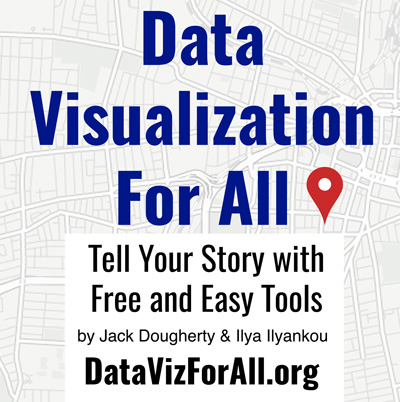
\includegraphics{images/0-introduction/cover-400wide.jpg}

\textbf{This book-in-progress} was last updated on: 2020-03-05.

\hypertarget{tell-your-data-story-with-free-and-easy-to-learn-tools.}{%
\subsubsection*{Tell your data story with free and easy-to-learn tools.}\label{tell-your-data-story-with-free-and-easy-to-learn-tools.}}
\addcontentsline{toc}{subsubsection}{Tell your data story with free and easy-to-learn tools.}

\emph{Data Visualization for All}, an open-access textbook, shows how to design interactive charts and maps for your website. We begin with drag-and-drop tools and gradually work our way up to editing open-source code templates. This friendly introduction includes step-by-step tutorials, video screencasts, and real-world examples. Featured tools include Google Sheets, Tableau Public, Chart.js, Leaflet, GitHub, and more.

\href{authors}{About the authors and contributors} from \href{http://www.trincoll.edu}{Trinity College, Hartford CT}: Jack Dougherty, Ilya Ilyankou, Veronica X. Armendariz, Stacy Lam, and David Tatem.

\href{https://datavizforall.org}{Read for free online} (recommended) or download PDF/eBook editions (to come).

Open-source code for text, data, chart and map templates at \url{https://github.com/datavizforall}

Data Visualization for All is copyrighted
by Jack Dougherty and Ilya Ilyankou and contributors
and distributed under a Creative Commons BY-NC 4.0 International License.
You may freely share and modify this content for non-commercial purposes, with a source credit to http://DataVizForAll.org.

\hypertarget{what}{%
\section{What is Data Visualization?}\label{what}}

\emph{last updated February 28, 2017}

Data visualization is broadly defined as a method of encoding quantitative, relational, or spatial information into images. Classic examples include \href{https://en.wikipedia.org/wiki/Charles_Joseph_Minard}{Charles Menard's figurative map} of Napoleon's defeat and retreat during the Russian campaign of 1812, and \href{https://en.wikipedia.org/wiki/John_Snow}{John Snow's dot map} of cholera cases during the London epidemic of 1854.

\begin{figure}
\centering
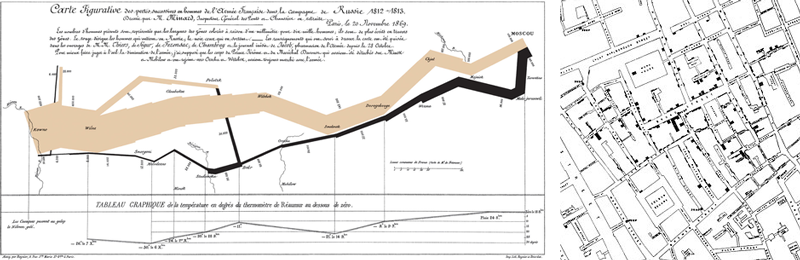
\includegraphics{images/0-introduction/examples-Minard-Snow.png}
\caption{Images: Menard's figurative map (left) and Snow's dot map (right), from Wikimedia}
\end{figure}

This free online introductory book focuses on selected topics in data visualization:

\textbf{Charts and maps} Despite the growing variety of visualization types, this book features chapters on creating \href{chart}{charts} and \href{map}{maps}, and a wide range of ways to communicate with these classic models.

\textbf{Reusable tools and templates:} Unlike infographics created for one-time use, all of the tools and templates in this book are recyclable, and allow you to upload a new dataset to display your story.

\textbf{Free and easy-to-learn:} We have selected data visualization tools that are free to use (or work on a freemium model, where advanced features or higher usage requires payment), and searched for those that we believe are easy-to-learn, based on our teaching experience with undergraduate students and non-profit community organizations.

\textbf{Interactive on the open web:} Many books assume that you will deliver your data visualizations to in-person audiences on printed paper or presentation slides. But in this book, we show how to \href{embed}{embed interactive charts and maps on your website}, to share with the wider public.

\textbf{Storytelling:} Data visualization is more than pretty pictures. In this book, the best visualizations are those that \href{story}{tell your data story} -- and pull readers' attention to what really matters -- by combining images and text, and offering exploration with explanation.

\hypertarget{learn-more}{%
\subsubsection*{Learn more}\label{learn-more}}
\addcontentsline{toc}{subsubsection}{Learn more}

\begin{itemize}
\tightlist
\item
  Michael Friendly and Daniel J. Denis, ``Milestones in the History of Thematic Cartography, Statistical Graphics, and Data Visualization,'' 2001, \url{http://www.datavis.ca/milestones/}
\item
  Isabel Meirelles, Design for Information: An Introduction to the Histories, Theories, and Best Practices Behind Effective Information Visualizations (Rockport Publishers, 2013), \url{http://isabelmeirelles.com/book-design-for-information/}
\item
  Edward Tufte, The Visual Display of Quantitative Information (Graphics Press, 1983), and subsequent works at \url{https://www.edwardtufte.com}
\end{itemize}

\hypertarget{why}{%
\section{Why this book?}\label{why}}

\emph{last updated February 20, 2017}

\emph{Data Visualization for All}, an open-access online textbook, seeks to help you tell your story -- and show your data -- through the power of the public web.

This open-access book reflects what I've learned while teaching data visualization \href{http://commons.trincoll.edu/dataviz}{to undergraduate students at Trinity College}, and now \href{https://www.edx.org/school/trinityx}{to a global online class on the Trinity edX platform}. Over the past few years, Trinity students and I have built interactive charts and maps in partnership with non-profit organizations in Hartford, Connecticut, to help them share their stories with data on the public web. Also, my students and colleagues have used these tools to create \href{http://ontheline.trincoll.edu}{On The Line: How Schooling, Housing, and Civil Rights Shaped Hartford and its Suburbs}, an open-access book-in-progress that features interactive historical maps of urban-suburban change. Students and colleagues who wrote tutorials, designed learning exercises, or developed code templates for \emph{Data Visualization for All} are listed as \href{authors}{authors and contributors}.

Although my outstanding colleagues have professional training, do not confuse them with me, the proverbial ``Jack of all trades, master of none.'' I do not consider myself an expert in data visualization, nor should anyone mistake me for a computer scientist or data scientist. Inspect my higher education transcripts and you'll see only one computer science class (something called FORTRAN77 back in 1982), and not a single course in statistics, sadly. Instead, my desire to learn data visualization was driven by my need as an historian to tell stories about urban-suburban places and change over time. If you've ever watched me teach a class or deliver a presentation on these topics -- always talking with my hands in the air -- you'll understand my primal need to create charts and maps. Stories become more persuasive when supported with data, especially well-crafted images that convey data relationships more clearly than words. Furthermore, these data stories become more powerful when we share them online, where they reach broader audiences who can interact with and evaluate our evidence.

In the early 2000s, when I began to dabble in data visualization, our tools were expensive, not easy to learn, and not designed to share our stories on the public web. (One of my well-worn jokes is point to the bald spot on my head, and claim that it was caused while tearing out my hair in frustration while using ArcGIS.) But everything began to change around 2005 when Google Maps publicly released its application programming interface (API) that allowed people with some coding skills to show data points on an interactive web map. Gradually, between 2008-11, I began learning what was possible by working on map projects with talented programmers and geographers, such as Jean-Pierre Haeberly at Trinity, and Michael Howser at the \href{http://magic.lib.uconn.edu/}{University of Connecticut Libraries Map and Geographic Information Center} (MAGIC, my favorite acronym), thanks to a grant from the \href{http://www.neh.gov}{National Endowment for the Humanities}. Free and low-cost workshops sponsored by \href{http://thatcamp.org}{The Humanities and Technology Camp} (THATCamp) at the Center for History and New Media at George Mason University, and \href{https://sunlightfoundation.com/transparency-camp/}{Transparency Camp} by the Sunlight Foundation, introduced me to many people (especially Mano Marks and Derek Eder) who demonstrated easier-to-use tools and templates, such as Google Fusion Tables and GitHub. Closer to home, Alvin Chang and other data journalists at the \href{http://ctmirror.org}{Connecticut Mirror} showed me how to tell stories on the web with more flexible open-source tools, such as Leaflet and Highcharts.

All of these data visualization lessons I learned have been \textbf{so valuable} -- to me, my students, our community partners, and thousands of readers on the web -- that my co-authors and I have agreed to share our knowledge with everyone, \textbf{for free}. This open-access book is guided by the principle of democratization of knowledge for the public good, hence the book's title: \emph{Data Visualization for All}. Not everyone can afford to make this choice, I realize. But the \href{http://www.trincoll.edu/AboutTrinity/mission/Pages/default.aspx}{mission of Trinity College} is to engage, connect, and transform, with both our local city of Hartford and the world at large. Since Trinity already pays my salary as a tenured professor, the right thing to do with the knowledge my students and I have gained is to pay it forward. That's why we created \emph{Data Visualization for All.}

If this free book is valuable for your education, then join us by sharing and supporting it for future readers:
- Tell your friends about the book and share the link via social media, text, or email
- Improve the book by adding comments or suggesting new chapters on our GitBook platform

Try out the tutorials, explore the online examples, share what you've learned with others, and dream about better ways to tell your data stories.

\hypertarget{authors}{%
\section{Authors and Contributors}\label{authors}}

UPDATE THIS: Contributors to \emph{Data Visualization for All} are credited in the byline to specific pages they authored (or co-authored), hold the copyright to those pages (jointly if co-authored), and have agreed to freely share the work as an open-access book. \emph{Data Visualization for All} is copyrighted by Jack Dougherty and contributors and distributed under a \href{http://creativecommons.org/licenses/by-nc/4.0/}{Creative Commons BY-NC 4.0 International License}. You may freely share and modify this content for non-commercial purposes, with a source credit to: \url{http://DataVizForAll.org}

\begin{longtable}[]{@{}ll@{}}
\toprule
\begin{minipage}[b]{0.50\columnwidth}\raggedright
Co-Authors\strut
\end{minipage} & \begin{minipage}[b]{0.44\columnwidth}\raggedright
About Us\strut
\end{minipage}\tabularnewline
\midrule
\endhead
\begin{minipage}[t]{0.50\columnwidth}\raggedright

\includegraphics{images/0-introduction/DoughertyJack-96.jpg}\strut
\end{minipage} & \begin{minipage}[t]{0.44\columnwidth}\raggedright
\href{http://bit.ly/jackdougherty}{Jack Dougherty} is Professor of Educational Studies at Trinity College in Hartford, Connecticut. He and his \href{http://commons.trincoll.edu/dataviz}{DataViz students} partner with community organizations to help tell their data stories on the web. Follow him on \href{https://twitter.com/doughertyjack}{Twitter} and \href{https://github/com/jackdougherty}{on GitHub}.\strut
\end{minipage}\tabularnewline
\begin{minipage}[t]{0.50\columnwidth}\raggedright

\includegraphics{images/0-introduction/IlyankouIlya-96.jpg}\strut
\end{minipage} & \begin{minipage}[t]{0.44\columnwidth}\raggedright
\href{https://www.linkedin.com/in/ilya-ilyankou-a64675ab}{Ilya Ilyankou} is a Civic Technologist at Connecticut Data Collaborative. He has completed a double major in Computer Science and Studio Arts in the Class of 2018 at Trinity College. Ilya developed Leaflet and Chart.js code templates for this book. Visit \href{http://ilyankou.com}{his website} or follow him \href{https://github.com/ilyankou}{on GitHub}.\strut
\end{minipage}\tabularnewline
\begin{minipage}[t]{0.50\columnwidth}\raggedright
Contributors\strut
\end{minipage} & \begin{minipage}[t]{0.44\columnwidth}\raggedright
\strut
\end{minipage}\tabularnewline
\begin{minipage}[t]{0.50\columnwidth}\raggedright

\includegraphics{images/0-introduction/ArmendarizVeronica-96.jpg}\strut
\end{minipage} & \begin{minipage}[t]{0.44\columnwidth}\raggedright
\href{https://www.linkedin.com/in/veronica-armendariz-4b814899}{Veronica X. Armendariz} earned her bachelor's degree in Educational Studies in 2016 from Trinity College, where she also served as a teaching assistant for the \href{http://commons.trincoll.edu/dataviz}{DataViz internship seminar}. She contributed tutorials for this book.\strut
\end{minipage}\tabularnewline
\begin{minipage}[t]{0.50\columnwidth}\raggedright

\includegraphics{images/0-introduction/LamStacy-96.jpg}\strut
\end{minipage} & \begin{minipage}[t]{0.44\columnwidth}\raggedright
Stacy Lam is a co-instructor for the \href{http://www.datavizforall.org/enroll}{Data Visualization for All online course} at Trinity College, where she is a prospective Engineering major in the Class of 2019. She contributed to chapters for this book.\strut
\end{minipage}\tabularnewline
\begin{minipage}[t]{0.50\columnwidth}\raggedright

\includegraphics{images/0-introduction/TatemDavid-96.jpg}\strut
\end{minipage} & \begin{minipage}[t]{0.44\columnwidth}\raggedright
\href{http://www.trincoll.edu/LITC/its/about/Pages/Learn.aspx}{David Tatem} is a co-instructor for the \href{http://www.datavizforall.org/enroll}{Data Visualization for All online course} at Trinity College, where he is an Instructional Technologist who specializes in the Social Sciences. He contributed to chapters for this book.\strut
\end{minipage}\tabularnewline
\bottomrule
\end{longtable}

Funding for student contributions to this book was generously provided by the \href{https://cher.trincoll.edu/community-learning/}{Community Learning Initiative} and \href{https://www.trincoll.edu/LITC/its/}{Information Technology Services} at \href{http://www.trincoll.edu}{Trinity College in Hartford, Connecticut}.

Live videos were produced with Trinity College Information Technology staff and friends: Angie Wolf, Sean Donnelly, Ron Perkins, Samuel Oyebefun, Phil Duffy, and Christopher Brown.

\hypertarget{trademarks}{%
\subsubsection*{Trademarks}\label{trademarks}}
\addcontentsline{toc}{subsubsection}{Trademarks}

Any use of a trademarked name without a trademark symbol is for readability purposes only. We have no intention of infringing on the trademark.

\begin{itemize}
\tightlist
\item
  CARTO is a registered trademark of CartoDB, Inc.
\item
  GitBook is a registered trademark of FriendCode, Inc.
\item
  GitHub and the GitHub logo are registered trademarks of GitHub, Inc.
\item
  Google and the Google logo are registered trademarks of Google Inc.
\item
  Social Explorer is a registered trademark of Social Explorer, Inc.
\item
  WordPress is a registered trademark of the WordPress Foundation
\end{itemize}

\hypertarget{disclaimer}{%
\subsubsection*{Disclaimer}\label{disclaimer}}
\addcontentsline{toc}{subsubsection}{Disclaimer}

The information is this book is provided without warranty. The lead author, contributors, and publisher have neither liability nor responsibility to any person or entity related to any loss or damages arising from the information contained in this book.

\hypertarget{read}{%
\section{How to Read}\label{read}}

\emph{last updated March 5, 2020}

\emph{Data Visualization for All} refers to both this open-access digital book and a \href{https://www.edx.org/course/data-visualization-for-all}{free online course} by the same name. We refer to them as ``the book'' and ``the course.''

This open-access book-in-progress is freely available in \textbf{two formats:} Web and PDF. \textbf{Read the online Web edition} at (\url{http://datavizforall.org}) to fully experience the interactive charts, maps, and video clips. Any modern web browser will display the book, but readers may prefer larger screens (desktop, laptop, tablet) over smaller screens (such as smartphones). In your web browser, try these toolbar features near the top of the page:

\begin{itemize}
\tightlist
\item
  Menu
\item
  Search
\item
  Font to adjust text size and display
\item
  View source code on GitHub
\item
  Download PDF
\item
  Shortcuts (arrow keys to navigate; \texttt{s} to toggle sidebar; \texttt{f} to toggle search)
\item
  Social Media
\item
  Share
\end{itemize}


\includegraphics{images/0-introduction/how-to-read.png}
A second option is to freely download the PDF edition \textbf{INSERT LINK}, which you can print out on paper for off-line reading. Although static images will appear in place of interactive maps and videos, the text and source notes in the PDF version are nearly identical to the web version. Since this digital-first has been created primarily for the web, some aspects of the book-in-progress may appear incomplete in the PDF edition. After the final manuscript is completed, a cleaner PDF version will be formatted, which the publisher will use to create an inexpensive paperback edition for sale.

\hypertarget{open-links-in-new-tabs}{%
\subsubsection*{Open links in new tabs}\label{open-links-in-new-tabs}}
\addcontentsline{toc}{subsubsection}{Open links in new tabs}

Keep your place when reading online and moving between pages.\\
- Two-finger trackpad click
- or Control + click (Mac)
- or Alt + click (Chromebook)
- or right-click (Windows and others)

\begin{figure}
\centering
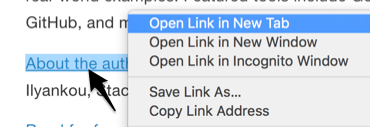
\includegraphics{images/0-introduction/contextual-menu.png}
\caption{Screenshot: Open link in new tab (on Mac)}
\end{figure}

\hypertarget{use-a-second-monitor}{%
\subsubsection*{Use a second monitor}\label{use-a-second-monitor}}
\addcontentsline{toc}{subsubsection}{Use a second monitor}

If you have a small screen, consider connecting a second monitor, or work next to a second computer or tablet. This allows you to view tutorials in one screen and build visualizations in the other screen.

\begin{figure}
\centering
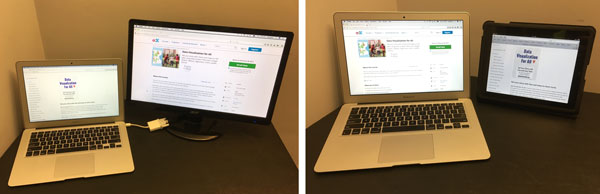
\includegraphics{images/0-introduction/laptop-and-monitor-and-tablet.jpg}
\caption{Image: Laptop with second monitor, and with tablet}
\end{figure}

\hypertarget{refresh-browser}{%
\subsubsection*{Refresh browser}\label{refresh-browser}}
\addcontentsline{toc}{subsubsection}{Refresh browser}

To view the most up-to-date content in your web browser, do a ``hard refresh'' to \href{https://en.wikipedia.org/wiki/Wikipedia:Bypass_your_cache}{bypass any saved content in your browser cache}.
- Ctrl + F5 (most Windows-Linux browsers)
- Command + Shift + R (Chrome or Firefox for Mac)
- Shift + Reload button toolbar (Safari for Mac)

\hypertarget{choose}{%
\chapter{Choose Tools to Tell Your Data Story}\label{choose}}

\emph{by \href{authors}{Jack Dougherty with Stacy Lam and David Tatem}, last updated February 10, 2017}

Do you feel overwhelmed by the enormous range of data visualization tools? There's been so many different tools released in recent years that anyone would have a hard time deciding which ones to use. Even if you limit your choices to the dozen or so tools specifically mentioned in this book, how do you make wise decisions?

\begin{itemize}
\tightlist
\item
  \href{draw}{Draw and Write Your Data Story} reminds us to start with the most important item in your toolkit: \textbf{\emph{your story}}. Begin by drawing pictures and writing questions or sentences to capture your ideas on paper, and then choose the most appropriate tools to create your vision.
\item
  \href{ask}{Ask Questions When Choosing Tools} lists several criteria to consider when making software decisions. Many of us look for free or affordable tools in the perfect sweet spot---easy-to-learn, yet powerful---and that's the focus of this book.
\item
  \href{rate}{Rate Three Simple Map Tools} invites readers to create a basic interactive point map using three different online tools, and to evaluate each one using selected criteria from the chapter above.
\end{itemize}

Enroll in our free online course \textbf{TO DO add link}, which introduces these topics in the brief video below, and offers more exercises and opportunities to interact with instructors and other learners.

\hypertarget{watch-the-youtube-video}{%
\subsubsection*{Watch the YouTube Video}\label{watch-the-youtube-video}}
\addcontentsline{toc}{subsubsection}{Watch the YouTube Video}

\hypertarget{draw}{%
\section{Draw and Write Your Data Story}\label{draw}}

\emph{last updated February 20, 2017}

Before you dive deeply into software, think about the most important item in your toolkit: \textbf{your story}. The primary reason we're designing visualizations is to improve how we communicate our data story to other people, so let's begin there.

Push away the computer and pick up some old-school tools:

\begin{itemize}
\tightlist
\item
  colored markers or pencils
\item
  lots of blank paper
\item
  your imagination
\end{itemize}

First, at the top of the page, write down your data story.

\begin{itemize}
\tightlist
\item
  Is it in the form of a question? If so, figure out how to pose the question.
\item
  Or maybe it's in the form of an answer to that question? If so, spell out your clearest statement.
\item
  If you're lucky, perhaps you already can envision a full story, with a beginning, middle, and end.
\item
  Whatever form it takes in your head, write out the words that come to mind.
\end{itemize}

Further down the page (or on a separate sheet), draw quick pictures of the visualizations that comes to your mind, even if you don't yet have any data. No artistic skills are required. Just use your imagination.
- Do you envision some type of chart? Sketch a picture.
- Or do you imagine some type of map? Show what it might look like.
- Will your visualization be interactive? Insert arrows, buttons, whatever.

Finally, share your data story with someone else and talk through your preliminary ideas. Does your sketch and sentences help to convey the broader idea that you're trying to communicate? If so, this is one good sign that your data story is worth pursuing, with the visualization tools, templates, and techniques in other chapters of this book.

\hypertarget{ask}{%
\section{Ask Questions When Choosing Tools}\label{ask}}

\emph{last updated February 6, 2017}

When each of us decides which digital tools best fit our needs, we often face trade-offs. On one hand, many of us prefer easy-to-learn tools, especially those with a drag-and-drop interface, but they often force us to settle for limited options. On the other hand, we also favor powerful tools that allow us to control and customize our work, yet most of these require higher-level coding skills. The goal of this book is to find the best of both worlds: that ``sweet spot'' where tools are both friendly and flexible.

\begin{figure}
\centering

\includegraphics{images/01-choose/tool-sweet-spot.png}
\caption{Diagram: the `sweet spot' for easy-to-learn and powerful tools}
\end{figure}

Before testing out new tools, try listing the criteria that guide your decision-making process. What are the most important factors that influence whether or not you add another item to your digital toolkit? Here's the list that came to our minds:

\textbf{\emph{1) Price:}} Is the tool free, or is there a ``freemium'' model to pay for more features or higher usage?

\textbf{\emph{2) Easy-to-learn:}} Is the tool relatively simple for new users without coding skills?

\textbf{\emph{3) Power:}} Does the tool support large amounts of data, and various types of visualizations?

\textbf{\emph{4) Customization:}} Can I modify details about how my work appears?

\textbf{\emph{5) Data Migration:}} Can I easily move my data in and out, in case I switch to a different tool?

Hint for historians: Future-proof your digital history projects! Choose tools that allow you to easily export and migrate data to other platforms. Design projects to keep your data separate from its digital presentation.

*** 6) Hosting:*** Can I decide exactly where my data and visualizations will be stored online?

*** 7) Support:*** Is the tool actively maintained by its creators, and do they answer questions?

*** 8) Open Source:*** Is the tool's software visible, can it be modified, and redistributed?

*** 9) Security:*** Is the tool and my data protected from malicious hackers and malware?

*** 10) Collaborative:*** Does the tool allow several people to work together on one shared product?

*** 11) Privacy:*** Under the terms of service, is my data and work private or public?

*** 12) Error-friendly:*** When something fails, does the tool point out possible problems and solutions?

*** 13) Cross-platform:*** Does this tool work across different computer operating systems?

*** 14) Mobile-friendly:*** Will it correctly display my work on various mobile devices and browsers?

That's a long list! It's even longer than the number of tools we'll mention in this book. But don't let it overwhelm you. The diagram at the top of the page illustrates the two most important criteria for the many free tools that are currently available: easy-to-learn and powerful features.

\hypertarget{learn-more-about-choosing-tools}{%
\subsubsection*{Learn more about choosing tools}\label{learn-more-about-choosing-tools}}
\addcontentsline{toc}{subsubsection}{Learn more about choosing tools}

Carl V. Lewis, Dataviz.tools: A curated guide to the best tools, resources and technologies for data visualization, \url{http://dataviz.tools}

Lincoln Mullen, ``How to Make Prudent Choices About Your Tools,'' ProfHacker blog, Chronicle of Higher Education, August 14, 2013, \url{http://www.chronicle.com/blogs/profhacker/how-to-make-prudent-choices-about-your-tools}

Lisa Charlotte Rost, ``What I Learned Recreating One Chart Using 24 Tools,'' Source, December 8, 2016, \url{https://source.opennews.org/en-US/articles/what-i-learned-recreating-one-chart-using-24-tools/}

Lisa Spiro and colleagues, DiRT: Digital Research Tools Directory (formerly Bamboo), \url{http://dirtdirectory.org}

Audrey Watters, ``\,`The Audrey Test': Or, What Should Every Techie Know About Education?,'' Hack Education, March 17, 2012, \url{http://hackeducation.com/2012/03/17/what-every-techie-should-know-about-education}

\hypertarget{rate}{%
\section{Rate Three Simple Map Tools}\label{rate}}

\emph{last updated March 16, 2017}

Let's explore criteria from the previous chapter by comparing three different tools, and reflecting on which factors you feel are most important when making decisions about your toolkit. We'll test three drag-and-drop tools to transform sample address data into a simple interactive point map.

Each tool can \textbf{geocode} address data by looking up a location (such as 500 Main Street, Hartford CT) in a large database, deciding on the best match, and converting this data into latitude and longitude coordinates (such as 41.762, -72.674).

For our sample data, we'll use this table of 9 locations in North America, with 3 intentional mistakes to test for geocoding errors.

\begin{figure}
\centering
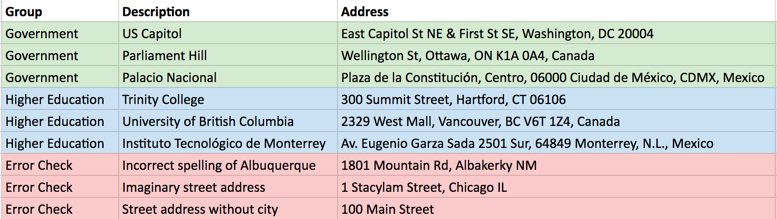
\includegraphics{images/01-choose/sample-address-screenshot.png}
\caption{Image: Sample address data screenshot}
\end{figure}

First, click this link and Save to download the sample file to your computer: \href{data/sample-address-data.csv}{sample-address-data in CSV format}. CSV means comma-separated-values, a generic spreadsheet format that many tools can easily open. If you need help with downloading, see this \href{https://www.youtube.com/watch?v=-04PQldP9HQ}{short video tutorial}.

Next, build a point map with the sample data, by following the tutorials for the three tools below.

\begin{longtable}[]{@{}ll@{}}
\toprule
Tool & Step-by-step tutorial in this book\tabularnewline
\midrule
\endhead
\href{https://www.google.com/maps/d/}{Google My Maps} & \href{mymaps}{My Maps tutorial}\tabularnewline
\href{http://carto.com}{Carto Builder} & \href{carto}{Carto tutorial}\tabularnewline
\bottomrule
\end{longtable}

Finally, rate your experience using each tool with these selected criteria:

\begin{itemize}
\tightlist
\item
  Easy-to-learn: Which tool was the simplest for creating a basic point map?
\item
  Price: Which of these free tools provided the most services at no cost?
\item
  Customization: Which tool enabled you to modify the most details about your map?
\item
  Data Migration: Which tool most easily allowed you to import and export your data?
\item
  Error-friendly: Which tool geocoded most accurately or signaled possible errors?
\end{itemize}

Recommended: Enroll in our free online course \textbf{LINK TO DO} to compare your ratings to other students.

\hypertarget{spreadsheet}{%
\chapter{Improve Your Spreadsheet Skills}\label{spreadsheet}}

\emph{by \href{authors}{Jack Dougherty}, last updated March 1, 2017}

Spreadsheets are wonderful tools to organize data into tables of rows and columns. With a spreadsheet, you can sort, filter, calculate, aggregate, and reorganize information to help you find the stories buried inside.

Four common spreadsheet tools:

\begin{longtable}[]{@{}ll@{}}
\toprule
\begin{minipage}[b]{0.47\columnwidth}\raggedright
Tool\strut
\end{minipage} & \begin{minipage}[b]{0.47\columnwidth}\raggedright
Features\strut
\end{minipage}\tabularnewline
\midrule
\endhead
\begin{minipage}[t]{0.47\columnwidth}\raggedright
\href{https://www.google.com/sheets/about/}{Google Sheets}\strut
\end{minipage} & \begin{minipage}[t]{0.47\columnwidth}\raggedright
Free, online collaborative spreadsheet on Google Drive. Requires free account.\strut
\end{minipage}\tabularnewline
\begin{minipage}[t]{0.47\columnwidth}\raggedright
\href{https://office.live.com/start/Excel.aspx}{Microsoft Excel Online}\strut
\end{minipage} & \begin{minipage}[t]{0.47\columnwidth}\raggedright
Free online spreadsheet on Microsoft OneDrive. Requires free account. Cannot open CSV generic spreadsheet files.\strut
\end{minipage}\tabularnewline
\begin{minipage}[t]{0.47\columnwidth}\raggedright
\href{https://products.office.com/en-us/excel}{Microsoft Excel desktop}\strut
\end{minipage} & \begin{minipage}[t]{0.47\columnwidth}\raggedright
Not free (US \$100+) spreadsheet for Mac or Windows desktop, as part of Microsoft Office.\strut
\end{minipage}\tabularnewline
\begin{minipage}[t]{0.47\columnwidth}\raggedright
\href{http://www.libreoffice.org}{LibreOffice}\strut
\end{minipage} & \begin{minipage}[t]{0.47\columnwidth}\raggedright
Free, open-source alternative to Microsoft Office desktop. Donation requested during download.\strut
\end{minipage}\tabularnewline
\bottomrule
\end{longtable}

Which spreadsheet tool should you use? That depends on how you wish to share and store data for your project.

\begin{itemize}
\tightlist
\item
  If you are the \textbf{only person} working on a data project, use any spreadsheet tool.
\item
  If you need to \textbf{protect private data}, avoid online tools and use any desktop spreadsheet.
\item
  If you need to \textbf{share live data} with others, use Google Sheets.
\end{itemize}

This introductory online book features Google Sheets because it's a free and easy-to-learn tool for collaborating and sharing data with others. The basic spreadsheet methods shown here are very similar across all spreadsheet tools. But advanced users may need more complex tools to manage very large datasets, or relational databases, or to perform deeper analysis.

If you're new to spreadsheets or want to refresh your skills, see the following chapters:

\begin{itemize}
\tightlist
\item
  \href{upload}{Upload and Convert to Google Sheets}
\item
  \href{copy}{Make a Copy with Google Sheets}
\item
  \href{share}{Share with Google Sheets}
\item
  \href{csv}{Save as CSV or ODS Format}
\item
  \href{sort}{Sort and Filter Data}
\item
  \href{calculate}{Calculate with Formulas}
\item
  \href{pivot}{Group Data with Pivot Tables}
\item
  \href{vlookup}{Match Data with VLookup}
\item
  \href{forms}{Collect and Share Survey Data with Google Forms}
\end{itemize}

Enroll in our free online course{]} which offers more spreadsheet exercises and opportunities to interact with instructors and other learners.

\hypertarget{upload}{%
\section{Upload Files and Convert to Google Sheets}\label{upload}}

\emph{last updated March 2, 2017}

Google Drive can convert many file types into \href{https://www.google.com/sheets/about/}{Google Sheets format}:

\begin{itemize}
\tightlist
\item
  Microsoft Excel (.xls and .xlsx)
\item
  OpenDocument Spreadsheet (.ods)
\item
  Comma-separated values (.csv)
\item
  Tab-separated values (.tab)
\item
  Text files (.txt) into Google Sheets format
\end{itemize}

\hypertarget{tutorial}{%
\subsubsection*{Tutorial}\label{tutorial}}
\addcontentsline{toc}{subsubsection}{Tutorial}

\begin{enumerate}
\def\labelenumi{\arabic{enumi})}
\item
  Sign in to your free Google Drive account (\url{http://drive.google.com})
\item
  To convert files into Google Sheets format, open the Settings (upper-right gear symbol), and \textbf{check the box} to Convert uploaded files to Google Docs.
\end{enumerate}

\begin{figure}
\centering
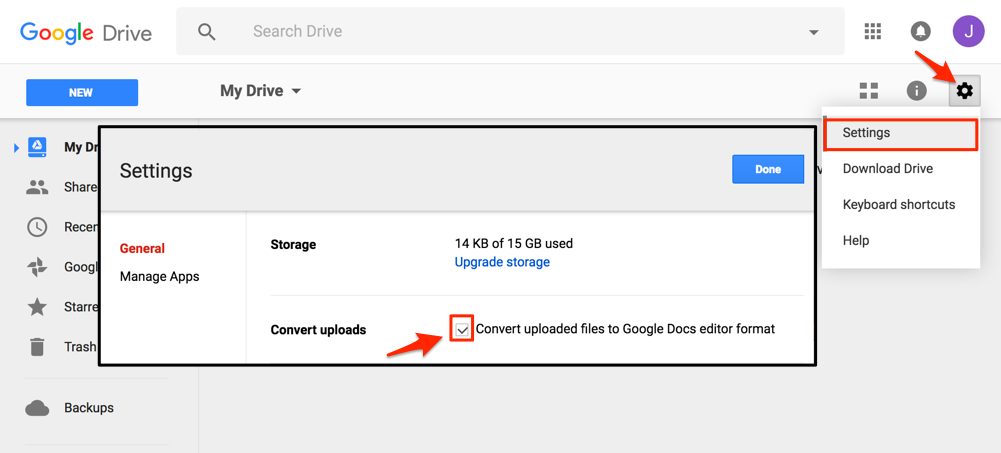
\includegraphics{images/02-spreadsheet/google-drive-settings-convert-uploads.png}
\caption{Screenshot: Check the box to Convert uploaded files to Google Docs format}
\end{figure}

\begin{enumerate}
\def\labelenumi{\arabic{enumi})}
\setcounter{enumi}{2}
\tightlist
\item
  To upload your file, use the New \textgreater{} File Upload menu OR drag-and-drop it into your Google Drive screen.
\end{enumerate}

\begin{figure}
\centering
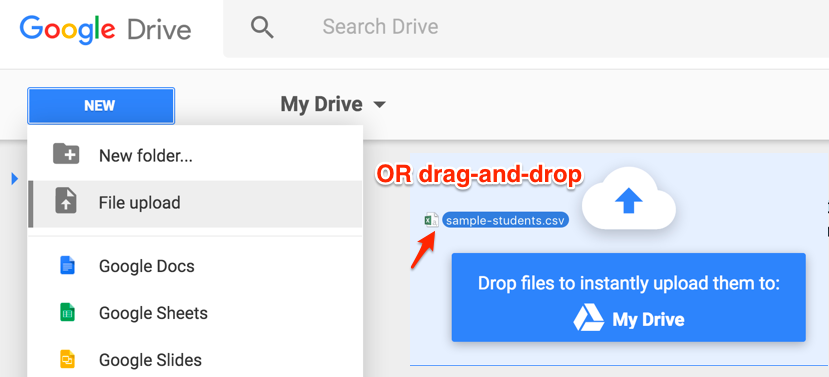
\includegraphics{images/02-spreadsheet/google-drive-upload-methods.png}
\caption{Screenshot: New \textgreater{} File upload OR Drag-and-drop the file}
\end{figure}

\begin{enumerate}
\def\labelenumi{\arabic{enumi})}
\setcounter{enumi}{3}
\tightlist
\item
  When your file is successfully converted, the Google Sheets icon will appear. Recommended: Right-click to rename the file and remove the old extension (.xlsx or .csv or other), since it is no longer in this old format.
\end{enumerate}

\begin{figure}
\centering
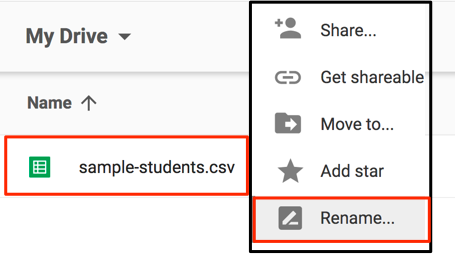
\includegraphics{images/02-spreadsheet/google-drive-sheets-icon-rename.png}
\caption{Screenshot: Right-click the Google Sheets icon to remove old file extension}
\end{figure}

\begin{enumerate}
\def\labelenumi{\arabic{enumi})}
\setcounter{enumi}{4}
\tightlist
\item
  Google Drive files that display different icons have \textbf{not} been converted into Google Sheets format.
\end{enumerate}

\begin{figure}
\centering
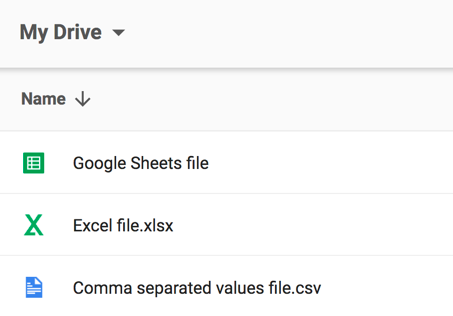
\includegraphics{images/02-spreadsheet/google-drive-spreadsheet-icons.png}
\caption{Screenshot: Spreadsheet format icons in Google Drive}
\end{figure}

\textbf{Beware}: A different way to convert spreadsheets into Google Sheets format is the File \textgreater{} Import menu, but this creates two files in your Google Drive (such as data and data.csv), which is confusing.

\hypertarget{copy}{%
\section{Make a Copy with Google Sheets}\label{copy}}

\emph{last updated March 17, 2017}

In this book, you will open links to Google Sheets that allow you to view -- but not edit -- the contents. How can you quickly make your own version that you can edit?

\begin{figure}
\centering
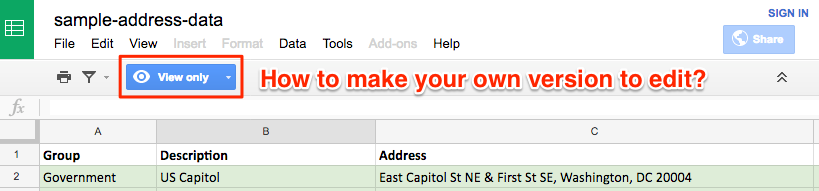
\includegraphics{images/02-spreadsheet/google-sheets-copy1.png}
\caption{Screenshot: View-only in Google Sheets}
\end{figure}

\hypertarget{best-solution}{%
\subsubsection*{Best solution}\label{best-solution}}
\addcontentsline{toc}{subsubsection}{Best solution}

\begin{enumerate}
\def\labelenumi{\arabic{enumi})}
\item
  Sign in to your Google account in the upper-right corner. Requires a free account.
\item
  Go to File \textgreater{} Make a Copy to save a duplicate of the spreadsheet to your Google Drive. By default, your copy will be private to you. Go to the \href{spreadsheet.html\#share}{Share Data with Google Sheets} chapter in this book to allow others to view, comment, or edit your spreadsheet.
\end{enumerate}

Highly recommended: Create folders in your Google Drive to keep your files organized and easily findable.

\begin{figure}
\centering
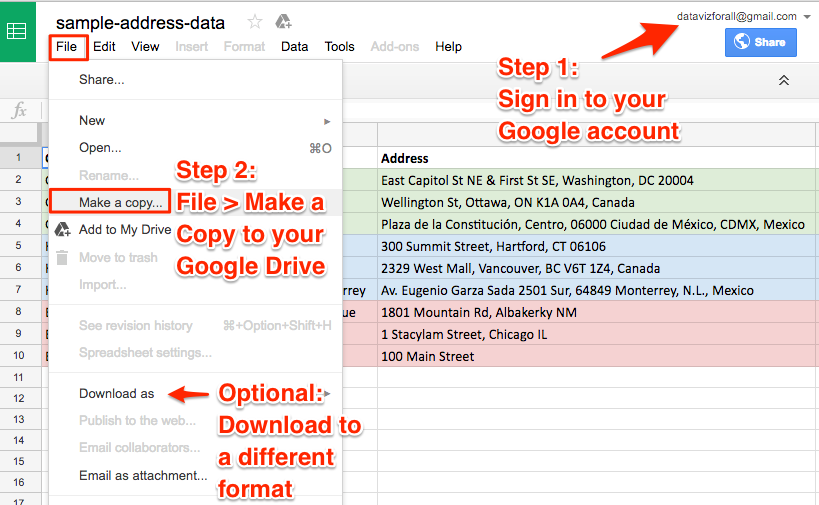
\includegraphics{images/02-spreadsheet/google-sheets-copy2.png}
\caption{Screenshot: Sign in and File \textgreater{} Make a Copy in Google Sheets}
\end{figure}

\hypertarget{alternate-solution}{%
\subsubsection*{Alternate solution}\label{alternate-solution}}
\addcontentsline{toc}{subsubsection}{Alternate solution}

Another option is to File \textgreater{} Download As into a different format, such as:
- Microsoft Excel (.xlsx)
- OpenData System (.ods), a generic multi-tab spreadsheet
- Comma-separated values (.csv), a generic single sheet
No Google account is required.

\hypertarget{share}{%
\section{Share Data with Google Sheets}\label{share}}

\emph{last updated March 1, 2017}

To share live spreadsheet data with other people, use Google Sheets (\url{https://www.google.com/sheets/about/}). Requires a free Google
Drive account.

\hypertarget{video-with-step-by-step-tutorial}{%
\subsubsection*{Video with step-by-step tutorial}\label{video-with-step-by-step-tutorial}}
\addcontentsline{toc}{subsubsection}{Video with step-by-step tutorial}

\begin{enumerate}
\def\labelenumi{\arabic{enumi})}
\item
  Sign in to your Google Drive (\url{http://drive.google.com}), and in the New menu, select Google Sheets.
\item
  New spreadsheets are private by default. Only the owner can view and edit.
\item
  To open your spreadsheet to others, click the blue Share button.
\item
  To share data with specific individuals, enter their Google usernames.
\item
  Or, to share data more widely, click the \textbf{Advanced} button on the next screen. (I wish Google made this button larger!)
\item
  Click the Change button and decide on Link Sharing settings:
\end{enumerate}

\begin{itemize}
\tightlist
\item
  Public on the web (anyone can find your data)
\item
  Anyone with the link (similar to an unlisted phone number)
\item
  Off (only specific people you list by Google usernames)
\end{itemize}

Below those settings, select the Access level:
- Can view
- Can comment
- Can edit (for co-authored data)

\begin{enumerate}
\def\labelenumi{\arabic{enumi})}
\setcounter{enumi}{6}
\tightlist
\item
  Select Save, and scroll down on the next screen to select Done.
\end{enumerate}

\textbf{Tip:} To avoid sending a long Google Sheets link to others, use a free link-shortening service such as Bit.ly (\url{http://bit.ly}). Requires a free account.

\hypertarget{learn-more-1}{%
\subsubsection*{Learn more}\label{learn-more-1}}
\addcontentsline{toc}{subsubsection}{Learn more}

\begin{itemize}
\tightlist
\item
  ``Share Files from Google Drive,'' Google help page, \url{https://support.google.com/docs/answer/2494822}
\item
  Jack Dougherty, ``How to Co-Author and Peer Edit with Google Docs,'' Web Writing: How and Why for Liberal Arts Teaching and Learning, (2015), \url{http://epress.trincoll.edu/webwriting/chapter/how-to-google-docs}
\end{itemize}

\hypertarget{csv}{%
\section{Save Spreadsheets in CSV or ODS}\label{csv}}

\begin{itemize}
\tightlist
\item
  last updated March 2, 2017*
\end{itemize}

To transfer spreadsheet data to another platform, or import it into a visualization tool, you may need to convert your file into a different format. Consider two options:

\hypertarget{comma-separated-values-.csv}{%
\subsubsection*{Comma-separated values (.csv)}\label{comma-separated-values-.csv}}
\addcontentsline{toc}{subsubsection}{Comma-separated values (.csv)}

\begin{itemize}
\tightlist
\item
  to transfer only one sheet of data, with no formulas or formatting, into a wide range of spreadsheet and visualization tools
\end{itemize}

\hypertarget{opendocument-spreadsheet-.ods}{%
\subsubsection*{OpenDocument Spreadsheet (.ods)}\label{opendocument-spreadsheet-.ods}}
\addcontentsline{toc}{subsubsection}{OpenDocument Spreadsheet (.ods)}

\begin{itemize}
\tightlist
\item
  to transfer multiple sheets, with basic formulas and formatting, into many spreadsheet tools (Excel, Google Sheets, LibreOffice)
\end{itemize}

\hypertarget{convert-to-csv-or-ods-with-google-sheets}{%
\subsubsection*{Convert to CSV or ODS with Google Sheets}\label{convert-to-csv-or-ods-with-google-sheets}}
\addcontentsline{toc}{subsubsection}{Convert to CSV or ODS with Google Sheets}

In the File \textgreater{} Download As menu, select either ODS (to convert a Google Sheets file with multiple tabs, formulas, and formatting) or CSV (to capture only the data in the current sheet).

\begin{figure}
\centering
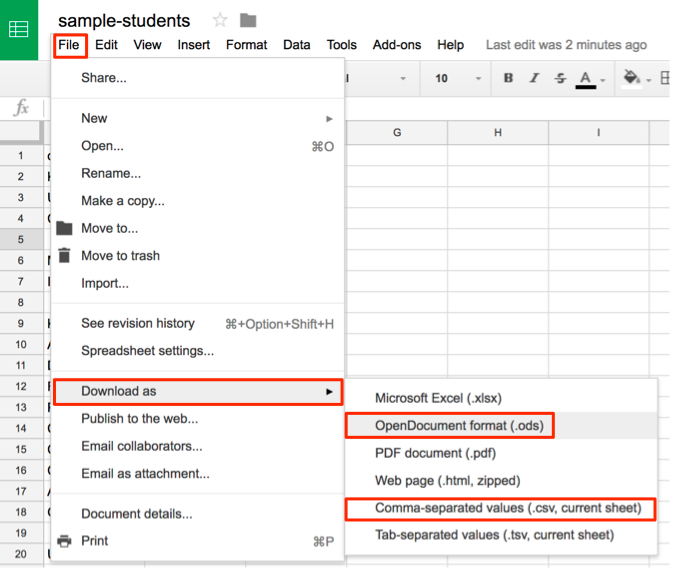
\includegraphics{images/02-spreadsheet/google-sheets-download-ods-csv.png}
\caption{Screenshot: Download Google Sheets data in ODS or CSV format}
\end{figure}

\hypertarget{convert-to-ods-with-microsoft-excel}{%
\subsubsection*{Convert to ODS with Microsoft Excel}\label{convert-to-ods-with-microsoft-excel}}
\addcontentsline{toc}{subsubsection}{Convert to ODS with Microsoft Excel}

In the File \textgreater{} Save As menu, select ODS format.

\begin{figure}
\centering
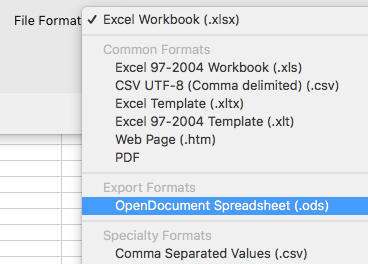
\includegraphics{images/02-spreadsheet/excel-save-as-ods.png}
\caption{Screenshot: Save as ODS with Excel for Mac}
\end{figure}

\hypertarget{convert-to-csv-with-microsoft-excel}{%
\subsubsection*{Convert to CSV with Microsoft Excel}\label{convert-to-csv-with-microsoft-excel}}
\addcontentsline{toc}{subsubsection}{Convert to CSV with Microsoft Excel}

\begin{enumerate}
\def\labelenumi{\arabic{enumi})}
\tightlist
\item
  Note that CSV format will save only the first sheet of a multi-sheet Excel workbook. If you have source information or other data in other tabs, keep your original Excel file for backup purposes. You can give them parallel file names:
\end{enumerate}

\begin{itemize}
\tightlist
\item
  data.csv
\item
  data.xlsx
\end{itemize}

\begin{enumerate}
\def\labelenumi{\arabic{enumi})}
\setcounter{enumi}{1}
\tightlist
\item
  In the Excel file, select the File \textgreater{} Save As menu, and select CSV format.
\end{enumerate}

\begin{figure}
\centering
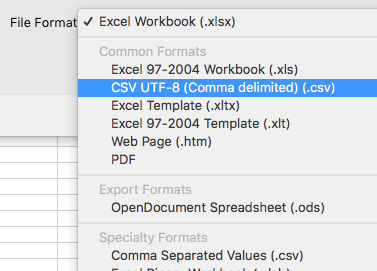
\includegraphics{images/02-spreadsheet/excel-save-as-csv.png}
\caption{Screenshot: Save as CSV in Excel for Mac}
\end{figure}

\begin{enumerate}
\def\labelenumi{\arabic{enumi})}
\setcounter{enumi}{2}
\tightlist
\item
  Older versions of Excel may warn you that some features (such as formulas and formatting) will not be saved in a generic CSV data file. Be sure to keep a backup Excel version, then click Continue to save your data into CSV format.
\end{enumerate}

\begin{figure}
\centering
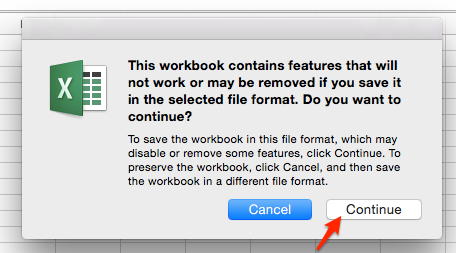
\includegraphics{images/02-spreadsheet/excel-save-as-csv-continue.png}
\caption{Screenshot: Older Excel warning before saving in CSV format}
\end{figure}

\begin{enumerate}
\def\labelenumi{\arabic{enumi})}
\setcounter{enumi}{3}
\tightlist
\item
  In older versions of Excel, when you quit the application, another screen will ask if you wish to save the CSV file a second time. \textbf{Don't let Excel confuse you.} If you have not made any changes to the Excel file since the step above, click Don't Save, because you already saved the file in CSV format.
\end{enumerate}

\begin{figure}
\centering
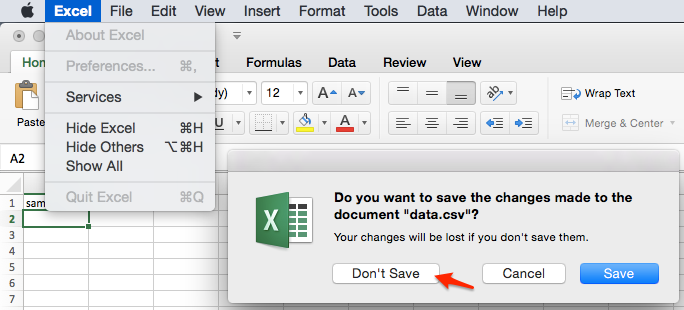
\includegraphics{images/02-spreadsheet/excel-quit-csv.png}
\caption{Screenshot: Older Excel version: click Don't Save}
\end{figure}

\hypertarget{sort}{%
\section{Sort and Filter Data}\label{sort}}

\emph{last updated January 13, 2017}

\textbf{TO DO}
- write intro on the title concepts
- when possible, start text by posing a common problem, and how this method can solve it
- redo visuals: Google Sheets with better example
- add Filter data

\hypertarget{sort-data-by-columns}{%
\subsubsection*{Sort data by columns}\label{sort-data-by-columns}}
\addcontentsline{toc}{subsubsection}{Sort data by columns}

To sort data rows by a column, select the entire spreadsheet (top-left corner icon), then right-click or look for the sort menu. Be sure to select the entire sheet to avoid accidentally sorting one column without the adjacent ones.


\includegraphics{images/placeholder.jpg}

\hypertarget{filter-data-by-columns}{%
\subsubsection*{Filter data by columns}\label{filter-data-by-columns}}
\addcontentsline{toc}{subsubsection}{Filter data by columns}

TO DO

\hypertarget{calculate}{%
\section{Calculate with Formulas and Functions}\label{calculate}}

\emph{last updated March 16, 2016}

\textbf{TO DO}
- when possible, start text by posing a common problem, and how this method can solve it
- redo visuals: Google Sheets with better examples
- see other notes inserted below

Simple formulas can save you lots of time. The big advantage of spreadsheet tools is the ability to insert simple formulas to calculate numbers, or combine columns of text, for entire rows and columns.

\hypertarget{write-a-simple-formula}{%
\subsubsection*{Write a simple formula}\label{write-a-simple-formula}}
\addcontentsline{toc}{subsubsection}{Write a simple formula}

In most spreadsheets, begin writing a simple formula with an equal sign, and refer to specific cells and functions, such as:

\begin{itemize}
\tightlist
\item
  = A2 + B2 + C2
\end{itemize}

\hypertarget{write-formulas-with-built-in-functions}{%
\subsubsection*{Write formulas with built-in functions}\label{write-formulas-with-built-in-functions}}
\addcontentsline{toc}{subsubsection}{Write formulas with built-in functions}

\textbf{TO DO} rewrite to show how this is same as above

\begin{itemize}
\tightlist
\item
  = Sum(A2:C2)
\end{itemize}

** TO DO ** rewrite to show common numerical and textual functions

\begin{itemize}
\tightlist
\item
  = Average(A2:C2)
\end{itemize}

\hypertarget{copy-and-paste-or-drag-formulas}{%
\subsubsection*{Copy and paste, or drag formulas}\label{copy-and-paste-or-drag-formulas}}
\addcontentsline{toc}{subsubsection}{Copy and paste, or drag formulas}

If you've inserted a formula into one row, how can you quickly do the same calculation across all rows?

Spreadsheets can magically automate calculations across rows or columns. In most cases, you can copy and paste a formula into new cells. Sometimes you can click-and-drag the lower-right corner of a formula cell (which may appear as a cross-hair) to automate calculations.


\includegraphics{images/placeholder.jpg}

\hypertarget{copy-and-paste-special-values-to-replace-formulas-with-data}{%
\subsubsection*{Copy and Paste \textgreater{} Special \textgreater{} Values to replace formulas with data}\label{copy-and-paste-special-values-to-replace-formulas-with-data}}
\addcontentsline{toc}{subsubsection}{Copy and Paste \textgreater{} Special \textgreater{} Values to replace formulas with data}

After inserting calculations in a spreadsheet, sometimes dynamic formulas must be replaced with static data before the results can be visualized. One solution is to select and copy a column (or the entire sheet), then paste \textgreater{} special \textgreater{} values to replace the formula with numerical results.


\includegraphics{images/placeholder.jpg}

Remember that if you need to check or run the calculations again at a later point, click (or right-click) the tab to save a copy to the spreadsheet as a backup.

\hypertarget{create-a-column-of-consecutive-numbers}{%
\subsubsection*{Create a column of consecutive numbers}\label{create-a-column-of-consecutive-numbers}}
\addcontentsline{toc}{subsubsection}{Create a column of consecutive numbers}

To quickly create a column of consecutive numbers, such as unique ID numbers, in most spreadsheet tools:

\begin{itemize}
\tightlist
\item
  Insert the number 1 into a cell and press Return
\item
  Click the cell and float the cursor over the bottom-right corner, where it will change into a cross-hair symbol
\item
  On a Mac, hold down the Option key and drag the cross-hair down to create consecutive numbers
\item
  \textbf{TO DO} insert equivalent commands for Windows, Chromebook
\end{itemize}


\includegraphics{images/placeholder.jpg}

\hypertarget{pivot}{%
\section{Group Data with Pivot Tables}\label{pivot}}

\emph{last updated March 16, 2017}

Here's a common problem: You open a large spreadsheet with many rows of data, such as a list of students. Your goal is to count students by categories, such as the number of students by each year of birth. What's the most efficient way to do this?

\begin{figure}
\centering
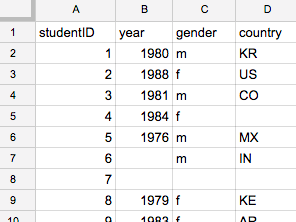
\includegraphics{images/02-spreadsheet/spreadsheet-pivot-intro.png}
\caption{Screenshot: Long spreadsheet of student data}
\end{figure}

A solution: Create a pivot table to aggregate (or group together) and summarize data in another spreadsheet tab.

\begin{figure}
\centering
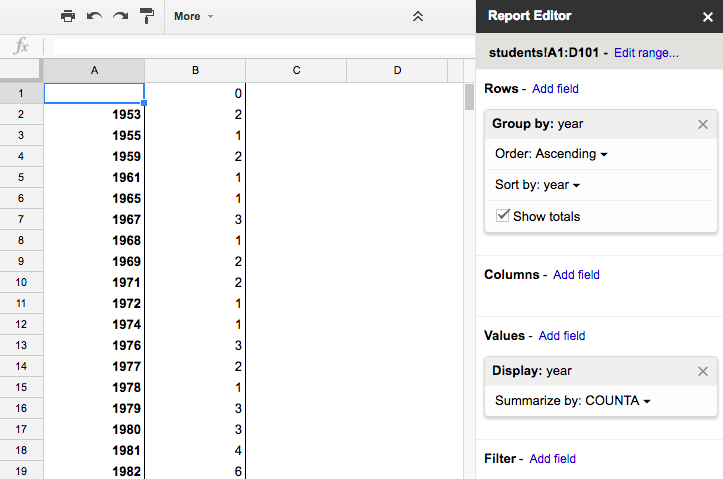
\includegraphics{images/02-spreadsheet/spreadsheet-google-pivot-year.png}
\caption{Screenshot: Pivot table of count by year of birth}
\end{figure}

While pivot tables may look different across spreadsheet tools, the concept is the same.

\hypertarget{video-with-step-by-step-tutorial-for-google-sheets}{%
\subsubsection*{Video with step-by-step tutorial for Google Sheets}\label{video-with-step-by-step-tutorial-for-google-sheets}}
\addcontentsline{toc}{subsubsection}{Video with step-by-step tutorial for Google Sheets}

\begin{enumerate}
\def\labelenumi{\arabic{enumi})}
\item
  Click this link and Save to download to your computer: \href{data/sample-students.csv}{sample-students in CSV format}. CSV means comma-separated values, a generic spreadsheet format that most tools can easily open.
\item
  Sign into \href{http://drive.google.com}{Google Drive} (requires free account) and drag-and-drop the sample CSV file to instantly upload. Before you do this, make sure your Settings (gear symbol) is set to Convert Uploads to Google Docs editor format (the default setting).
\item
  Shift-click to select all columns that you wish to pivot.
\item
  Select Data \textgreater{} Pivot Table\ldots, which opens a new spreadsheet tab.
\item
  In Report Editor, select Rows \textgreater{} Add Field \textgreater{} Year to list all entries in order.
\item
  In Report Editor, select Values \textgreater{} Add Field \textgreater{} Year to summarize all values for each entry.
\item
  Change Summarize by SUM to Summarize by COUNTA (to count alphabetical or numerical entries), or COUNT (to count only numeric values).
\end{enumerate}

\hypertarget{more-advanced-pivot-table-with-google-sheets}{%
\subsubsection*{More Advanced Pivot Table with Google Sheets}\label{more-advanced-pivot-table-with-google-sheets}}
\addcontentsline{toc}{subsubsection}{More Advanced Pivot Table with Google Sheets}

In addition to grouping by rows, you can create more advanced pivot tables by grouping by columns and filtering results. For example, the pivot table shown below shows rows by birth year, columns by gender (blank, female, male, other), and filters results to show only 18 students from one country: US.

\begin{figure}
\centering
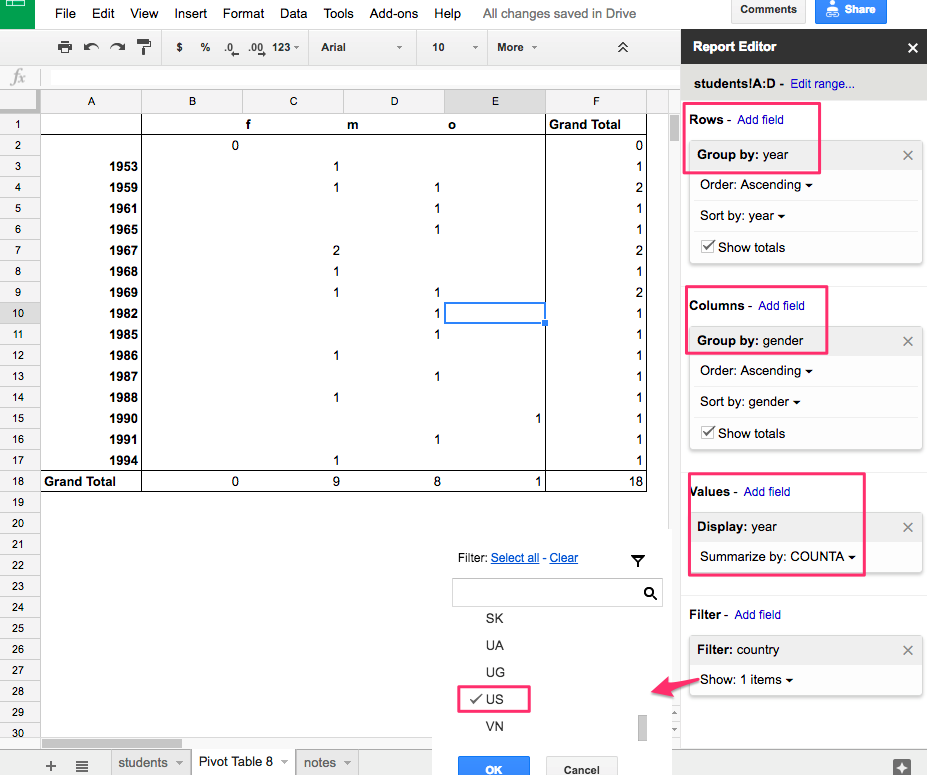
\includegraphics{images/02-spreadsheet/spreadsheet-pivot-google-advanced.png}
\caption{Screenshot: Advanced pivot table by year of birth and gender for US}
\end{figure}

\hypertarget{learn-more-2}{%
\subsubsection*{Learn More}\label{learn-more-2}}
\addcontentsline{toc}{subsubsection}{Learn More}

\begin{itemize}
\tightlist
\item
  Google, Create and Use Pivot Tables Help Page \url{https://support.google.com/docs/answer/1272898}
\item
  LibreOffice, Creating Pivot Tables Help Page \url{https://help.libreoffice.org/Calc/Creating_Pivot_Tables}
\item
  Andrew Ba Tran, ``Tutorial: How to Make Pivot Tables in Google Sheets,'' TrendCT, September 4, 2015, \url{http://trendct.org/2015/09/04/tutorial-how-to-make-pivot-tables-in-google-sheets}
\end{itemize}

\hypertarget{vlookup}{%
\section{Match Columns with VLOOKUP}\label{vlookup}}

\emph{last updated March 16, 2017}

Here's a common problem: Sheet 1 contains a long roster of students enrolled in our \emph{Data Visualization For All} course, with a two-letter code for their nation. Sheet 2 contains the list of codes for each nation. How can we quickly match up this information in one sheet, so that each row contains the nation for each student?

\begin{figure}
\centering
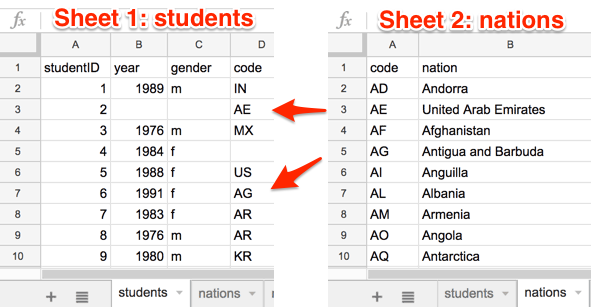
\includegraphics{images/02-spreadsheet/vlookup-problem.png}
\caption{Screenshot: Problem - How to match columns in two sheets?}
\end{figure}

One solution: Spreadsheets contain a VLOOKUP function, which ``looks up'' data across two or more vertical columns, and automatically fills in matching entries. This tutorial demonstrates how to set up this calculation in Google Sheets and Excel

\begin{figure}
\centering
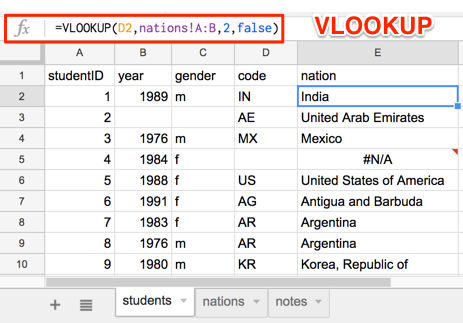
\includegraphics{images/02-spreadsheet/vlookup-solution.png}
\caption{Screenshot: Solution - Use the VLookup function}
\end{figure}

\hypertarget{video-with-step-by-step-tutorial-for-google-sheets-1}{%
\subsubsection*{Video with step-by-step tutorial for Google Sheets}\label{video-with-step-by-step-tutorial-for-google-sheets-1}}
\addcontentsline{toc}{subsubsection}{Video with step-by-step tutorial for Google Sheets}

\begin{enumerate}
\def\labelenumi{\arabic{enumi})}
\item
  Click this link and Save to download to your computer: \href{data/sample-students-nations.ods}{sample-students-nations in .ODS format}. ODS means OpenDocument System, a generic multi-tab format that most spreadsheet tools can easily open.
\item
  To upload the downloaded file to Google Sheets, see the \href{upload}{Upload Files and Convert tutorial} in this book, and remember that Settings (gear symbol) must be set to Convert files to Google format. Or, open the file with Microsoft Excel or LibreOffice, and the directions below will be similar.
\item
  In the students sheet, type ``nation'' as a column header into cell E1.
\item
  Click in cell E2, start typing ``=VLOOKUP'' and the spreadsheet tool will suggest that you complete the formula in this format:
\end{enumerate}

\begin{Shaded}
\begin{Highlighting}[]
\NormalTok{VLOOKUP(search\_key, range, index, [is\_sorted])}
\end{Highlighting}
\end{Shaded}

\begin{itemize}
\tightlist
\item
  search\_key = the Sheet 1 cell we are trying to match
\item
  range = the columns in Sheet 2 where matches may exist
\item
  index = the column in the Sheet 2 range that contains the desired result, where 1 = first column, 2 = second column, etc.
\item
  {[}is\_sorted{]} = if the first column of the range is sorted, enter ``true'' to find the closest match; otherwise enter ``false'' to return exact matches only
\end{itemize}

\begin{enumerate}
\def\labelenumi{\arabic{enumi})}
\setcounter{enumi}{3}
\tightlist
\item
  You can type in the formula, or fill it out by clicking on cells, columns, and sheets as shown in the video above.
\end{enumerate}

\hypertarget{forms}{%
\section{Collect and Share Data with Google Forms}\label{forms}}

\textbf{TO DO } write simple tutorial for Google Forms and explain how to share the spreadsheet; also mention other web form services

\hypertarget{find}{%
\chapter{Find and Know Your Data}\label{find}}

\emph{by \href{authors}{Jack Dougherty}, last updated March 1, 2017}

\hypertarget{searching-for-open-data}{%
\subsubsection*{Searching for Open Data}\label{searching-for-open-data}}
\addcontentsline{toc}{subsubsection}{Searching for Open Data}

Increasing numbers of governmental agencies and non-profit organizations are publicly sharing \emph{open data} on the web. When starting a new data visualization project, ask yourself these questions:

\begin{itemize}
\tightlist
\item
  Do I have the most relevant data for my project?
\item
  Is it the most current data, in the most user-friendly format?
\item
  Is data available at the individual level, or aggregated into larger groups?
\item
  Which organizations might have collected data for my topic?
\item
  Which open data repositories might have published this data?
\end{itemize}

\hypertarget{what-features-do-open-repositories-offer}{%
\subsubsection{What features do open repositories offer?}\label{what-features-do-open-repositories-offer}}

\begin{itemize}
\tightlist
\item
  View and export: At minimum, most open data repositories allow users to view their data and export it into common spreadsheet formats. Some also provide geographical boundaries for polygon maps.
\item
  Built-in visualization tools: Some repositories offer built-in tools for users to create interactive charts or maps on the platform site. Some also provide code snippets for users to embed these built-in visualizations into their own websites.
\item
  Static and Live data: Most repositories offer static datasets for a specific time period, but some also provide ``live'' data that is continuously updated.
\item
  Application Programming Interface (APIs): Some repositories provide endpoints with code instructions that allow users to pull data directly from the platform into an external sites or online visualization, which is ideal for continuously updated data.
\end{itemize}

\hypertarget{know-your-data}{%
\subsubsection{Know Your Data}\label{know-your-data}}

Before starting to create charts or maps, get to know your data.

\begin{itemize}
\tightlist
\item
  Where did it come from?
\item
  Who compiled the data, and for what purpose?
\item
  What do the data labels really mean?
\item
  Ask yourself: Am I working with the \emph{most} recent version, in the \emph{best} available format?
\end{itemize}

\textbf{TO DO} add resource \url{https://github.com/Quartz/bad-data-guide}

open data inception 1600+ sites portal
\url{http://opendatainception.io/}

\begin{itemize}
\tightlist
\item
  Know your data: go out into the field to directly observe how the original data is measured and collected
\end{itemize}

\url{https://www.opendatanetwork.com/}

Closely examine your data files to understand their meaning, sources of origin, and limitations.
\textbf{TO DO} expand on this theme with examples of bad and misleading data

\begin{enumerate}
\def\labelenumi{\arabic{enumi})}
\tightlist
\item
  Always ask: Am I using the best available data?
\end{enumerate}

\begin{itemize}
\tightlist
\item
  Compare the HFS list to the City of Hartford's current list of food establishments:
  \url{https://data.hartford.gov/browse}
\item
  go to Public Health Category
\item
  click on the ``dataset'' version (updated 10 Feb 2016), which is same data but different view than the ``map'' version
\item
  click on light blue ``export'' button into any format you wish to compare with the HFS list (see screenshot)
\item
  decide which list is best for your organization's goal
\end{itemize}

\hypertarget{census}{%
\section{US and Census Bureau Open Data}\label{census}}

\emph{By \href{authors}{Jack Dougherty and Ilya Ilyankou}, last updated December 25, 2019}

\textbf{The U.S. Census Bureau} (\url{https://census.gov}) collects and shares population, housing, and economic data on its open repositories.

\begin{itemize}
\tightlist
\item
  The Decennial Census is a full count of the population every ten years, most recently in 2010 and the upcoming one in 2020. Because decennial data are counts and not estimates, they represent ``true'' values and hence come without margins of errors.
\item
  The American Community Survey (ACS) (\url{https://www.census.gov/programs-surveys/acs/}) is annual sample count, which produces:

  \begin{itemize}
  \tightlist
  \item
    1-year estimates for areas with populations of 65,000+
  \item
    5-year estimates for all census areas
  \item
    ACS used to release 3-year estimates for geographies with population of 20,000+, but discontinued after the 2011-2013 release.
  \end{itemize}
\end{itemize}

Because ACS produces estimates and not ``true'' counts, data comes with margins of errors. Generally, margins of errors are higher for smaller geographies (eg census blocks) and smaller values (eg the number of Asian females aged 60+ who live in Union, CT). Hence, one needs to be critical when using ACS or other survey data.

\textbf{Census areas} are geographic divisions in this \emph{general format}:

\begin{itemize}
\tightlist
\item
  State
\item
  County
\item
  County subdivisions (equivalent to Connecticut towns and cities)
\item
  Census tracts (designated areas, roughly 2,500 to 8,000 people)
\item
  Block groups (sub-unit of tract, roughly 600 to 3,000 people)
\item
  Census blocks (sub-unit of block group, but not always a city block)
\end{itemize}

\hypertarget{census-areas-in-the-hartford-region}{%
\subsection{Census areas in the Hartford region}\label{census-areas-in-the-hartford-region}}

The interactive map below illustrates hierarchical relations among geographical census entities for the Hartford region, from state to census block level.

Learn more: Explore the standard hierarchy of US Census geographic entities and definitions (\url{https://www2.census.gov/geo/pdfs/reference/geodiagram.pdf})

See also in this book: \href{geocode}{Geocode addresses with the US Census Geocoder}

\hypertarget{data.census.gov}{%
\subsection{Data.census.gov}\label{data.census.gov}}

Data.census.gov (\url{https://data.census.gov}) is the main platform to access US Census data. It provides an easy search across census and survey tables. There is an interface to view tables for various years and geographies, and a download button to save data as CSV or PDF. It replaced American FactFinder (\url{https://factfinder.census.gov}) in July 2019.

\hypertarget{social-explorer}{%
\subsection{Social Explorer}\label{social-explorer}}

\textbf{Social Explorer} (\url{https://www.socialexplorer.com/}) is a popular tool to view and download census and related demographic data, past and present. The platform allows users to create data maps that may be exported as static images or presentation slides. Social Explorer requires subscription, but many academic institutions provide access.

\textbf{TO DO} create tutorial on how to cleanly download census data from Social Explorer and Census.gov to join with geography, especially census tract numbers

\hypertarget{data.gov}{%
\subsection{Data.gov}\label{data.gov}}

\textbf{Data.gov} (\url{https://www.data.gov/}) is the official open data repository for US federal government agencies, managed by the US General Services Administration, and powered by an open-source CKAN and WordPress platform.

\hypertarget{national-center-for-education-statistics}{%
\subsection{National Center for Education Statistics}\label{national-center-for-education-statistics}}

\textbf{National Center for Education Statistics (NCES)} (\url{https://nces.ed.gov/}) is the primary federal agency for collecting and reporting education data.

\begin{itemize}
\tightlist
\item
  Elementary/Secondary Information System (ELSi) (\url{https://nces.ed.gov/ccd/elsi}) - create custom tables and charts from the Common Core of Data (CCD) and Private School Survey.
\end{itemize}

\hypertarget{boundaries}{%
\subsubsection*{Boundaries}\label{boundaries}}
\addcontentsline{toc}{subsubsection}{Boundaries}

** TO DO **
- link and source files and scale
- \url{http://mapstarter.com/}

\hypertarget{source}{%
\section{Source Your Data Files}\label{source}}

\emph{last updated March 1, 2017}

Source your data. Spell out exactly where it came from, so that someone other than you, several years in the future, could understand its origin.

\hypertarget{label-the-file-name}{%
\subsubsection*{Label the file name}\label{label-the-file-name}}
\addcontentsline{toc}{subsubsection}{Label the file name}

Everyone has seen examples of bad file names:

\begin{itemize}
\tightlist
\item
  data.xls
\item
  bldgdatalist.csv
\item
  data77.xls
\end{itemize}

Write a short but meaningful file name. It is a good idea to include data source in file name (eg \texttt{acs2018}, \texttt{worldbank}, or \texttt{eurostat}). If different versions of the data are floating around, add the current date at the end, in YYYY-MM-DD format. Good file names look like this:

\begin{itemize}
\tightlist
\item
  town-demographics-2019-12-02.xls
\item
  census2010\_population\_by\_county.csv
\item
  eurostat-1999-2019-CO2\_emissions.xlsx
\end{itemize}

\hypertarget{save-source-data-in-separate-sheet}{%
\subsubsection*{Save source data in separate sheet}\label{save-source-data-in-separate-sheet}}
\addcontentsline{toc}{subsubsection}{Save source data in separate sheet}

Before modifying the original dataset, make sure to duplicate it to avoid any data losses. One way is to click (or right-click) on the spreadsheet tab to copy the sheet to another tab as a backup.


\includegraphics{images/placeholder.jpg}

Add a \emph{source} tab, after the data, with notes to remind you and others about its origins and when it was last updated.

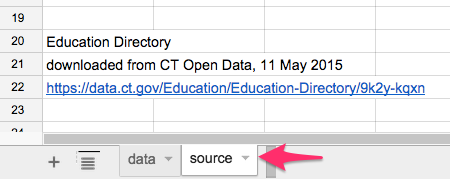
\includegraphics{images/03-find/SpreadsheetSourceTab.png}

\hypertarget{learn-more-3}{%
\subsection{Learn more}\label{learn-more-3}}

Lisa Charlotte Rost, \emph{How to prepare your data for analysis and charting in Excel \& Google Sheets},
\url{https://blog.datawrapper.de/prepare-and-clean-up-data-for-data-visualization/}

** TO DO **

Source your data

\begin{verbatim}
 - explain that data cannot be copyrighted, but representations of data can be
 - open-source and creative commons
 - credit sources and collaborators on dataviz products and readme files
 - Whose perspectives does your data privilege? Whose stories remain untold?
\end{verbatim}

\hypertarget{public}{%
\section{Public or Private Data?}\label{public}}

Many of the free web-based tools in this book require that your publicly share your data. Check each tool and decide whether it is appropriate for your data, which may have some privacy restrictions.

In some cases, individual data privacy is protected by law, but a government agency may aggregate (sort into larger groups) or anonymize (remove personally identifiable details) data to make it public. For example:

\begin{itemize}
\tightlist
\item
  Individual-level census data is private for about 70 years, but the US Census Bureau publicly releases anonymous data for aggregated areas (such as census blocks, tracts, towns, etc.)
\item
  Patient-level health records are private, but public health officials share town- and county-level health data.
\item
  Student-level education data is private, but school districts and state agencies publicly share grade-level and school-level data.
\end{itemize}

In other cases, individual data is not private. For example:

\begin{itemize}
\tightlist
\item
  When individuals contribute to political campaigns, most US and state laws require that the donor name, address, and amount is public data.
\item
  When an individual buys home in Connecticut, the owner's name, address, purchase amount, and other details about the home are public data.
\end{itemize}

\hypertarget{know}{%
\section{Know Your Data: Is It Good or Bad?}\label{know}}

Before starting to create charts or maps, get to know your data.

\begin{itemize}
\tightlist
\item
  Where did it come from?
\item
  Who compiled the data, and for what purpose?
\item
  What do the data labels really mean?
\item
  Ask yourself: Am I working with the \emph{most} recent version, in the \emph{best} available format?
\end{itemize}

Closely examine your data files to understand their meaning, sources of origin, and limitations.
\textbf{TO DO} expand on this theme with examples of bad and misleading data

** TO DO ** cite and explain this resource
\url{https://github.com/Quartz/bad-data-guide}

\hypertarget{learn-more-4}{%
\subsection{Learn more}\label{learn-more-4}}

Christopher Ingraham, \emph{An alarming number of scientific papers contain Excel errors},
\url{https://www.washingtonpost.com/news/wonk/wp/2016/08/26/an-alarming-number-of-scientific-papers-contain-excel-errors/}

\hypertarget{ct}{%
\section{Connecticut Open Data}\label{ct}}

\emph{last updated April 5, 2017}

Since this book was created in Hartford, Connecticut, we include state and municipal open data repositories and boundary files.

\textbf{Connecticut Open Data} (\url{http://data.ct.gov}), the official portal for state government agencies, is hosted on the Socrata platform, which offers built-in data visualization tools and APIs. See also how to create a \href{filtered-point-map-socrata}{filtered point map with Socrata} in this book.

See also separate repositories for individual state agencies:
- Office of the State Comptroller (\url{http://www.osc.ct.gov/openCT.html})
- CT State Department of Education (\url{http://www.sde.ct.gov/sde/cwp/view.asp?a=2758\&q=334520})
- Office of Policy and Management (\url{http://ct.gov/opm/cwp/view.asp?a=3006\&Q=383258\&opmNav_GID=1386})
- link to all CT state government agencies (\url{http://portal.ct.gov/Department-and-Agencies/})

\textbf{Connecticut State Data Center} (\url{http://ctsdc.uconn.edu/}), part of the U.S. Census Data Center Network, is the lead agency for US Census data and other socioeconomic data for Connecticut, and is based at the University of Connecticut Libraries. The site also features data visualizations created on the Tableau platform and provides population projections for the state of Connecticut.

\textbf{MAGIC: The Map and Geographic Information Center} (\url{http://magic.lib.uconn.edu}), based at the University of Connecticut Libraries, specializes in providing geographic, aerial photography, and map images for the state, past and present. The site also features interactive maps.

\textbf{DataHaven} (\url{http://ctdatahaven.org/}), a non-profit organization, collects and interprets information about Connecticut neighborhoods, such as its Community Wellbeing Survey. Data resources feature neighborhood profiles for densely-populated areas (New Haven and Hartford-West Hartford), and town profiles for other areas across the state.

\textbf{Connecticut Data Collaborative} (\url{http://ctdata.org}) is a public-private partnership that advocates for open data access to drive planning, policy, budgeting and decision making in Connecticut at the state, regional and local levels. We democratize public data through custom data exploration tools and a dynamic town profile tool, hosted on the open-source CKAN platform. Users can find state and federal data on topics such as public health, education, crime, municipal data, and racial profiling data.

\textbf{Hartford Data} (\url{http://data.hartford.gov}), the official portal of the City of Hartford municipal government, is hosted on the Socrata platform, which features built-in visualizations and APIs. See also how to create a \href{filtered-point-map-socrata}{filtered point map with Socrata} in this book. Also, the Hartford Data site links to the City's ArcGIS Online geographic data (\url{http://gisdata.hartford.gov/}) and the City's financial data (\url{http://checkbook.hartford.gov/}) and budget (\url{http://budget.hartford.gov/}).

In addition to the official repositories above, Connecticut news organizations that create data visualizations often include links to download data files.

\textbf{Connecticut Mirror / Trend CT } (\url{http://ctmirror.org/}) and (\url{http://trendct.org/}) are publications of the Connecticut News Project, an independent, nonpartisan, nonprofit organization that focuses on state policy issues. Most of their data visualizations are built with open-source code, with publicly accessible data files. See also their GitHub repository (\url{https://github.com/trendct}).

\textbf{Hartford Courant Data Desk} (\url{http://www.courant.com/data-desk}) produces digital visualizations for the \emph{Hartford Courant}, the largest daily newspaper in Connecticut, owned by Tribune Publishing. Many of these data visualizations are published on the Tableau platform, which allows readers to download the underlying data.

\hypertarget{boundaries-1}{%
\subsubsection*{Boundaries}\label{boundaries-1}}
\addcontentsline{toc}{subsubsection}{Boundaries}

\begin{itemize}
\tightlist
\item
  Converted from shapefile WGS84 to GeoJSON format
\item
  To download a GeoJSON file, right-click the link and Save to your computer
\item
  If you accidentally open the GeoJSON code in your browser, select File \textgreater{} Save Web Page to download it
\item
  To view or edit, drag files into \url{http://geojson.io} or \url{http://mapshaper.org}
\item
  Learn more in the \href{transform.html}{Transform Your Map Data} chapter of this book
\end{itemize}

\begin{longtable}[]{@{}llll@{}}
\toprule
\begin{minipage}[b]{0.28\columnwidth}\raggedright
Geography\strut
\end{minipage} & \begin{minipage}[b]{0.22\columnwidth}\raggedright
Year-Source-Size\strut
\end{minipage} & \begin{minipage}[b]{0.19\columnwidth}\raggedright
Right-click + Save to download GeoJSON\strut
\end{minipage} & \begin{minipage}[b]{0.19\columnwidth}\raggedright
\strut
\end{minipage}\tabularnewline
\midrule
\endhead
\begin{minipage}[t]{0.28\columnwidth}\raggedright
CT outline 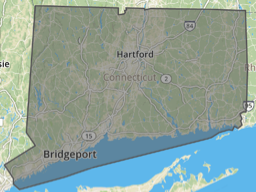
\includegraphics{data/ct-outline.png}\strut
\end{minipage} & \begin{minipage}[t]{0.22\columnwidth}\raggedright
\href{http://magic.lib.uconn.edu/connecticut_data.html\#boundaries}{2010 Census UConn MAGIC WGS84 1:100,000}\strut
\end{minipage} & \begin{minipage}[t]{0.19\columnwidth}\raggedright
\href{data/ct-outline.geojson}{ct-outline.geojson}\strut
\end{minipage} & \begin{minipage}[t]{0.19\columnwidth}\raggedright
\strut
\end{minipage}\tabularnewline
\begin{minipage}[t]{0.28\columnwidth}\raggedright
CT counties 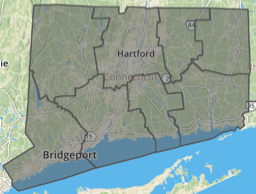
\includegraphics{data/ct-counties.png}\strut
\end{minipage} & \begin{minipage}[t]{0.22\columnwidth}\raggedright
\href{http://magic.lib.uconn.edu/connecticut_data.html\#boundaries}{2010 Census UConn MAGIC WGS84 1:100,000}\strut
\end{minipage} & \begin{minipage}[t]{0.19\columnwidth}\raggedright
\href{data/ct-counties.geojson}{ct-counties.geojson}\strut
\end{minipage} & \begin{minipage}[t]{0.19\columnwidth}\raggedright
\strut
\end{minipage}\tabularnewline
\begin{minipage}[t]{0.28\columnwidth}\raggedright
CT towns 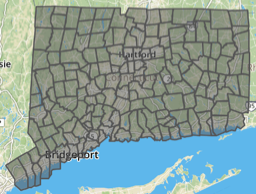
\includegraphics{data/ct-towns.png}\strut
\end{minipage} & \begin{minipage}[t]{0.22\columnwidth}\raggedright
\href{http://magic.lib.uconn.edu/connecticut_data.html\#boundaries}{2010 Census UConn MAGIC WGS84 simplified to 224k}\strut
\end{minipage} & \begin{minipage}[t]{0.19\columnwidth}\raggedright
\href{data/ct-towns.geojson}{ct-towns.geojson}\strut
\end{minipage} & \begin{minipage}[t]{0.19\columnwidth}\raggedright
\strut
\end{minipage}\tabularnewline
\begin{minipage}[t]{0.28\columnwidth}\raggedright
CT census tracts 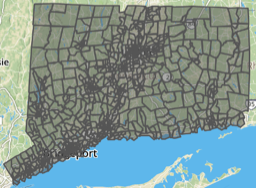
\includegraphics{data/ct-tracts-2010.png}\strut
\end{minipage} & \begin{minipage}[t]{0.22\columnwidth}\raggedright
\href{http://magic.lib.uconn.edu/connecticut_data.html\#boundaries}{2010 Census UConn MAGIC WGS84 1:100,000}\strut
\end{minipage} & \begin{minipage}[t]{0.19\columnwidth}\raggedright
\href{data/ct-tracts-2010.geojson}{ct-tracts-2010.geojson}\strut
\end{minipage} & \begin{minipage}[t]{0.19\columnwidth}\raggedright
\strut
\end{minipage}\tabularnewline
\begin{minipage}[t]{0.28\columnwidth}\raggedright
Hartford County outline 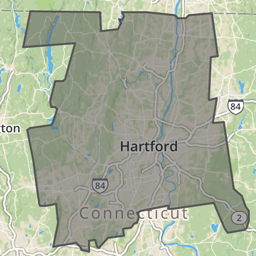
\includegraphics{data/hartfordcounty-outline.png}\strut
\end{minipage} & \begin{minipage}[t]{0.22\columnwidth}\raggedright
\href{http://magic.lib.uconn.edu/connecticut_data.html\#boundaries}{2010 Census UConn MAGIC WGS84 1:100,000}\strut
\end{minipage} & \begin{minipage}[t]{0.19\columnwidth}\raggedright
\href{data/hartfordcounty-outline.geojson}{hartfordcounty-outline.geojson}\strut
\end{minipage} & \begin{minipage}[t]{0.19\columnwidth}\raggedright
\strut
\end{minipage}\tabularnewline
\begin{minipage}[t]{0.28\columnwidth}\raggedright
Hartford County towns 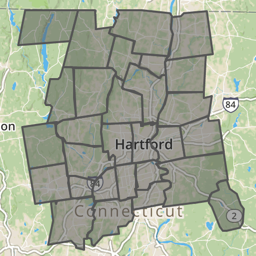
\includegraphics{data/hartfordcounty-towns.png}\strut
\end{minipage} & \begin{minipage}[t]{0.22\columnwidth}\raggedright
\href{http://magic.lib.uconn.edu/connecticut_data.html\#boundaries}{2010 Census UConn MAGIC WGS84 1:100,000}\strut
\end{minipage} & \begin{minipage}[t]{0.19\columnwidth}\raggedright
\href{data/hartfordcounty-towns.geojson}{hartfordcounty-towns.geojson}\strut
\end{minipage} & \begin{minipage}[t]{0.19\columnwidth}\raggedright
\strut
\end{minipage}\tabularnewline
\begin{minipage}[t]{0.28\columnwidth}\raggedright
Hartford County tracts 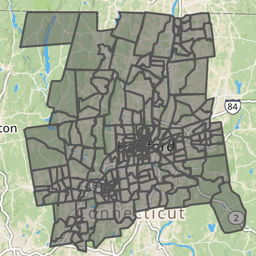
\includegraphics{data/hartfordcounty-tracts-2010.png}\strut
\end{minipage} & \begin{minipage}[t]{0.22\columnwidth}\raggedright
\href{http://magic.lib.uconn.edu/connecticut_data.html\#boundaries}{2010 Census UConn MAGIC WGS84 1:100,000}\strut
\end{minipage} & \begin{minipage}[t]{0.19\columnwidth}\raggedright
\href{data/hartfordcounty-tracts-2010.geojson}{hartfordcounty-tracts-2010.geojson}\strut
\end{minipage} & \begin{minipage}[t]{0.19\columnwidth}\raggedright
\strut
\end{minipage}\tabularnewline
\begin{minipage}[t]{0.28\columnwidth}\raggedright
Hartford outline 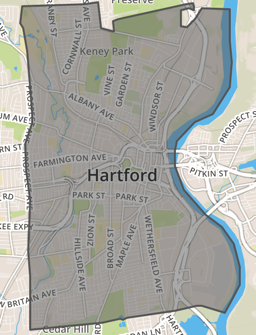
\includegraphics{hartford-outline.png}\strut
\end{minipage} & \begin{minipage}[t]{0.22\columnwidth}\raggedright
\href{http://magic.lib.uconn.edu/connecticut_data.html\#boundaries}{2010 Census UConn MAGIC WGS84 1:100,000}\strut
\end{minipage} & \begin{minipage}[t]{0.19\columnwidth}\raggedright
\href{data/hartford-outline.geojson}{hartford-outline.geojson}\strut
\end{minipage} & \begin{minipage}[t]{0.19\columnwidth}\raggedright
\strut
\end{minipage}\tabularnewline
\begin{minipage}[t]{0.28\columnwidth}\raggedright
Hartford census tracts 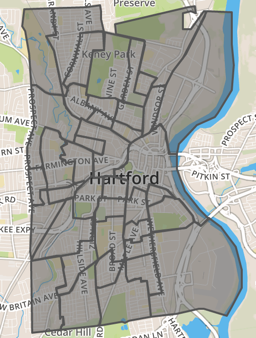
\includegraphics{data/hartford-tracts-2010.png}\strut
\end{minipage} & \begin{minipage}[t]{0.22\columnwidth}\raggedright
\href{http://magic.lib.uconn.edu/connecticut_data.html\#boundaries}{2010 Census UConn MAGIC WGS84 1:100,000}\strut
\end{minipage} & \begin{minipage}[t]{0.19\columnwidth}\raggedright
\href{data/hartford-tracts-2010.geojson}{hartford-tracts-2010.geojson}\strut
\end{minipage} & \begin{minipage}[t]{0.19\columnwidth}\raggedright
\strut
\end{minipage}\tabularnewline
\begin{minipage}[t]{0.28\columnwidth}\raggedright
Hartford neighborhoods 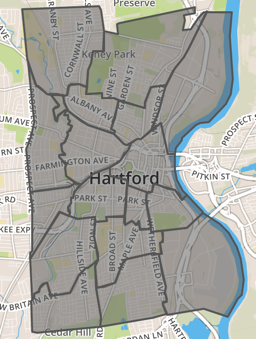
\includegraphics{data/hartford-neighborhoods.png}\strut
\end{minipage} & \begin{minipage}[t]{0.22\columnwidth}\raggedright
\href{http://gisdata.hartford.gov/datasets/d3deb11bfd9242ce9c927187c512da9e_5}{2015 Hartford Open Data 1:50,000}\strut
\end{minipage} & \begin{minipage}[t]{0.19\columnwidth}\raggedright
\href{data/hartford-neighborhoods.geojson}{hartford-neighborhoods.geojson}\strut
\end{minipage} & \begin{minipage}[t]{0.19\columnwidth}\raggedright
\strut
\end{minipage}\tabularnewline
\bottomrule
\end{longtable}

\textbf{TO DO}
- add Capitol Region Council of Governments (CRCOG) \url{http://www.crcog.org/}
- add school districts (and clarify elementary-secondary)
- add Capitol Region Education Council (CREC) \url{http://www.crec.org/}
- add school attendance areas from federal site
- describe Freedom of Information Act (FOIA) data requests in Connecticut

\hypertarget{clean}{%
\chapter{Clean Up Messy Data}\label{clean}}

\emph{By \href{authors}{Jack Dougherty}, last updated April 2016}

TO DO

\begin{itemize}
\tightlist
\item
  write a new intro to match content that I moved into subfolders
\item
  \url{http://trendct.org/2015/08/28/getting-rid-of-duplicate-rows-using-google-sheets/}
\item
  Clean up data that contains stray commas, or mistyped entries
\item
  Advanced clean up with Open Refine; see Alvin Chang's CT Mirror guide \url{http://trendct.org/2015/04/24/john-jonathan-and-johnny-how-to-merge-them-in-open-refine/}
\item
  rethink formatting data
\item
  see Jake Kara's ``Data Structure Whining'' \url{https://github.com/jakekara/publishing-data-for-journalists}
\end{itemize}

\hypertarget{clean-spreadsheets}{%
\section{Clean Data with Spreadsheets}\label{clean-spreadsheets}}

\emph{last updated April 16, 2016}

\textbf{TO DO} reorganize this to feature Google Sheets whenever possible, or Excel Online if needed

Sometimes we receive a spreadsheet with problematic data that needs to be cleaned up before we can successfully upload it into a visualization tool.

\hypertarget{find-and-replace-with-a-blank}{%
\subsubsection*{Find and Replace with a blank}\label{find-and-replace-with-a-blank}}
\addcontentsline{toc}{subsubsection}{Find and Replace with a blank}

A common problem with census data is that geographic names contain unnecessary words. For example, when downloading Connecticut county subdivisions (towns), each row appears as:

\begin{itemize}
\tightlist
\item
  Andover town
\item
  Ansonia town
\item
  Ashford town
\end{itemize}

Our goal is to remove the word ``town'' from each row, to produce a clean spreadsheet that we can match with other data, like this:

\begin{itemize}
\tightlist
\item
  Andover
\item
  Ansonia
\item
  Ashford
\end{itemize}

Here's one quick solution: In any spreadsheet tool, use the Find and Replace command to remove unwanted characters. Try it! Click this link and Save to download to your computer:\href{data/find-replace-town-geonames.csv}{find-replace-town-geonames in CSV format}. This tutorial shows screens from Excel, but other tools are very similar.

\begin{enumerate}
\def\labelenumi{\arabic{enumi}.}
\item
  Open the Find and Replace command.
\item
  In the Find field, type " town``, leaving a space before the word, since we wish to remove only that word when by itself. (Otherwise, we would accidentally remove the''town" in Newtown.)
\item
  In the Replace field, leave it blank, to represent a blank space.
\item
  Press the Replace All button. Since this sample file lists 169 towns, the screen will states that 169 instances of ``town'' have been replaced.
\end{enumerate}

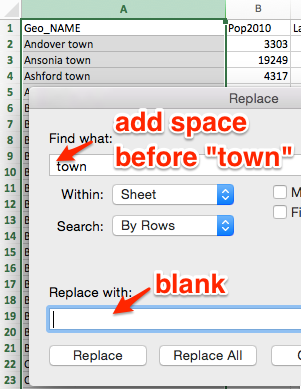
\includegraphics{images/04-clean/find-replace-blank.png}

\hypertarget{split-one-column-into-two-with-excel}{%
\subsubsection*{Split one column into two with Excel}\label{split-one-column-into-two-with-excel}}
\addcontentsline{toc}{subsubsection}{Split one column into two with Excel}

One common problem is when multiple pieces of data appear in one column, and your goal is to split them into separate columns. If those data pieces are separated by commas (or similar punctuation), you might be able to fix this with a simple spreadsheet command: split text into columns.

Try it! Click this link and Save to download to your computer: \href{data/split-coordinate-pairs.csv}{split-coordinate-pairs in CSV format}, and open with Excel. (\textbf{TO DO} test with other spreadsheet tools)

\begin{enumerate}
\def\labelenumi{\arabic{enumi}.}
\item
  Select the data column you wish to split.
\item
  Select Data \textgreater{} Split Text to Column
\item
  In the wizard screen, select Delimited data and click next.
\item
  In step 2 of the wizard screen, check the ``comma'' box, since this symbol divides the data column. Click next.
\item
  In step 3 of the wizard screen, accept the default General format, and Finish.
\end{enumerate}

The coordinate pairs column is now split into two separate columns. Relabel the headers: longitude and latitude.

Animated example from Excel for Windows (thanks \texttt{@f3mlat}):


\includegraphics{images/placeholder.jpg}

\textbf{TO DO} write directions to split a single address cell ``300 Summit St, Hartford CT 06106'' into separate columns for address, city, state, zip

\hypertarget{combine-separate-data-columns-into-one}{%
\subsubsection*{Combine separate data columns into one}\label{combine-separate-data-columns-into-one}}
\addcontentsline{toc}{subsubsection}{Combine separate data columns into one}

Another common data cleaning problem is when you receive address data in separate columns, like this:

\begin{longtable}[]{@{}llll@{}}
\toprule
Street & City & State & Zip\tabularnewline
\midrule
\endhead
100 Main St & Hartford & CT & 06106\tabularnewline
\bottomrule
\end{longtable}

But your data visualization tool requires you to combine all of this terms into one location column, like this:

\begin{longtable}[]{@{}l@{}}
\toprule
Location\tabularnewline
\midrule
\endhead
100 Main St, Hartford, CT 06106\tabularnewline
\bottomrule
\end{longtable}

One easy solution is to write a simple spreadsheet formula to combine (or concatenate) terms, using ampersands (\&) as connectors, and quotation marks around blank spaces as separators. For example, if a spreadsheet contained four columns, \emph{Address, City, State Zip} (A-D), then in column E insert a new header named \emph{Location} and a formula in this format:

\begin{itemize}
\tightlist
\item
  =A2 \&" " \& B2 \&" " \&C2 \&" " \&D2
\end{itemize}

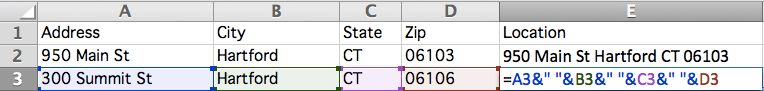
\includegraphics{images/04-clean/SpreadsheetCombineTerms.png}

\textbf{TO DO}
- Confirm that Google Fusion Tables geocoder does not require commas between terms
- Clarify what happens with zip code in the example above

\hypertarget{convert-connecticut-town-names-with-ctnamecleaner}{%
\subsubsection*{Convert Connecticut town names with CTNamecleaner}\label{convert-connecticut-town-names-with-ctnamecleaner}}
\addcontentsline{toc}{subsubsection}{Convert Connecticut town names with CTNamecleaner}

In Connecticut, residents often list their village or neighborhood names in their address, but these do not necessarily match the official list of 169 Connecticut town governments (called county subdivisions by the US Census). For example, the Elmwood neighborhood is located in the town of West Hartford, and the Rockville village is located in the town of Vernon.

To solve this problem, the data experts at TrendCT/CT Mirror have openly shared a wonderful tool to convert village/neighborhood names into official towns, called CTNamecleaner.

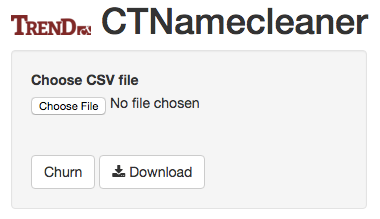
\includegraphics{images/04-clean/CTNamecleaner.png}

\begin{enumerate}
\def\labelenumi{\arabic{enumi}.}
\tightlist
\item
  Open CTNamecleaner with your browser at \url{http://shiny.trendct.org/ctnamecleaner/}
\item
  Upload a CSV generic spreadsheet. Learn more about CSV format in this book \textbf{TO DO add link}.
\item
  Select the data column to be converted into town names, and download the results.
\end{enumerate}

Learn more about \href{https://github.com/trendct/ctnamecleaner}{CTNamecleaner on GitHub}, and view the \href{https://docs.google.com/spreadsheets/d/1WqZIGk2AkHXKYvd4uXy5a2nwyg529e7mMU5610Ale0g/edit\#gid=0}{underlying list of Connecticut place names in a public Google sheet}.

\hypertarget{open-refine}{%
\section{Clean Data with Open Refine}\label{open-refine}}

\textbf{TO DO } show basic tutorial with Open Refine; link to Alvin Chang's fabulous \href{http://trendct.org/2015/04/24/john-jonathan-and-johnny-how-to-merge-them-in-open-refine/}{Open Refine tutorial in CT Mirror}

\hypertarget{ctnamecleaner}{%
\section{Fix Connecticut Town Names with CTNamecleaner}\label{ctnamecleaner}}

\emph{last updated April 16, 2016}

\textbf{TO DO} update this page; avoid duplication in main chapter text

Here's a wonderful data-cleaning tool that's specific to Connecticut, but the idea (and open-source code from TrendCT/CT Mirror) may inspire others to create similar tools for other locations.

In Connecticut, residents often list their village or neighborhood names in their address, but these do not necessarily match the official list of 169 Connecticut town governments (called county subdivisions by the US Census). For example, the Elmwood neighborhood is located in the town of West Hartford, and the Rockville village is located in the town of Vernon.

To solve this problem, the data experts at TrendCT/CT Mirror have openly shared a wonderful tool to convert village/neighborhood names into official towns, called CTNamecleaner.

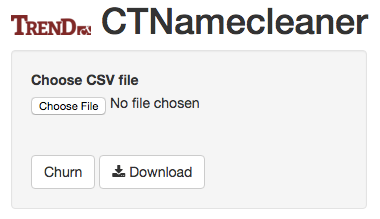
\includegraphics{images/04-clean/CTNamecleaner.png}

\begin{enumerate}
\def\labelenumi{\arabic{enumi}.}
\tightlist
\item
  Open CTNamecleaner with your browser at \url{http://shiny.trendct.org/ctnamecleaner/}
\item
  Upload a CSV generic spreadsheet. Learn more about CSV format in this book \textbf{TO DO} fix link
\item
  Select the data column to be converted into town names, and download the results.
\end{enumerate}

Learn more about \href{https://github.com/trendct/ctnamecleaner}{CTNamecleaner on GitHub}, and view the \href{https://docs.google.com/spreadsheets/d/1WqZIGk2AkHXKYvd4uXy5a2nwyg529e7mMU5610Ale0g/edit\#gid=0}{underlying list of Connecticut place names in a public Google sheet}.

\hypertarget{chart}{%
\chapter{Chart Your Data}\label{chart}}

\emph{by \href{authors}{Jack Dougherty}, last updated March 21, 2017}

Charts pull readers deeper into your story. Even if your data contains geographical information, sometimes a chart tells your story better than a map. But designing meaningful, interactive charts requires careful thought about how to communicate your data story with your audience. In this chapter, you will learn how to:

\begin{itemize}
\tightlist
\item
  Practice \href{chart-design}{principles of chart design}. Learn to identify good charts from bad ones.
\item
  Choose a chart type that matches your story and data format, and follow tutorials in the table below. Beginners may start with easy-to-learn tools such as \href{chart-google-sheets}{Google Sheets} or \href{tableau-public}{Tableau Public}, then move up to more powerful tools, such as \href{chartjs}{Chart.js}, which require you to \href{github}{Modify and Host Code Templates with GitHub} or another web host.
\end{itemize}

See also related chapters in this book:

\begin{itemize}
\tightlist
\item
  \href{draw}{Draw and write your data story} to capture your ideas on paper
\item
  \href{spreadsheet}{Improve spreadsheet skills}, \href{find}{Find and know your data}, and \href{clean}{Clean your data}
\item
  \href{embed}{Embed your interactive chart on your website}
\item
  \href{detect}{Detect bias in data stories}, including \href{how-to-lie-with-charts}{How to lie with charts}
\item
  \href{story}{Tell your data story}, including its most meaningful insights and limitations
\end{itemize}

\begin{longtable}[]{@{}ll@{}}
\toprule
\begin{minipage}[b]{0.47\columnwidth}\raggedright
Basic chart types\strut
\end{minipage} & \begin{minipage}[b]{0.47\columnwidth}\raggedright
Best use and tutorial chapters\strut
\end{minipage}\tabularnewline
\midrule
\endhead
\begin{minipage}[t]{0.47\columnwidth}\raggedright
Grouped column or bar 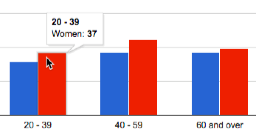
\includegraphics{images/05-chart/chart-grouped-column.png}\strut
\end{minipage} & \begin{minipage}[t]{0.47\columnwidth}\raggedright
Best to compare categories side-by-side. Vertical columns, or horizontal bars for long labels. Easy tool: \href{column-bar-google}{Google Sheets bar and column tutorial}Power tool: \href{highcharts}{Highcharts templates}\strut
\end{minipage}\tabularnewline
\begin{minipage}[t]{0.47\columnwidth}\raggedright
Separated column or bar \includegraphics{images/05-chart/chart-separated-column.png}\strut
\end{minipage} & \begin{minipage}[t]{0.47\columnwidth}\raggedright
Best to compare categories in separate clusters. Vertical columns, or horizontal bars for long labels.Easy tool: \href{column-bar-google}{Google Sheets bar and column tutorial}Power tool: \href{highcharts}{Highcharts templates}\strut
\end{minipage}\tabularnewline
\begin{minipage}[t]{0.47\columnwidth}\raggedright
Stacked column or bar \includegraphics{images/05-chart/chart-stacked-column.png}\strut
\end{minipage} & \begin{minipage}[t]{0.47\columnwidth}\raggedright
Best to compare sub-categories, or parts of a whole. Vertical columns, or horizontal bars for long labels.Easy tool: \href{column-bar-google}{Google Sheets bar and column tutorial}Power tool: \href{highcharts}{Highcharts templates}\strut
\end{minipage}\tabularnewline
\begin{minipage}[t]{0.47\columnwidth}\raggedright
Histogram \includegraphics{images/05-chart/chart-histogram.png}\strut
\end{minipage} & \begin{minipage}[t]{0.47\columnwidth}\raggedright
Best to show distribution of raw data, with number of values in each bucket.Easy tool: \href{column-bar-google}{Google Sheets bar and column tutorial}Power tool: \href{highcharts}{Highcharts templates}\strut
\end{minipage}\tabularnewline
\begin{minipage}[t]{0.47\columnwidth}\raggedright
Pie chart \includegraphics{images/05-chart/chart-pie.png}\strut
\end{minipage} & \begin{minipage}[t]{0.47\columnwidth}\raggedright
Best to show parts of a whole, but hard to estimate size of slices.Easy tool: \href{pie-line-area-google}{Google Sheets pie chart tutorial}Power tool: \href{highcharts}{Highcharts templates}\strut
\end{minipage}\tabularnewline
\begin{minipage}[t]{0.47\columnwidth}\raggedright
Line chart \includegraphics{images/05-chart/chart-line.png}\strut
\end{minipage} & \begin{minipage}[t]{0.47\columnwidth}\raggedright
Best to show continuous data, such as change over time.Easy tool: \href{pie-line-area-google}{Google Sheets line chart tutorial}Power tool: \href{highcharts}{Highcharts templates}\strut
\end{minipage}\tabularnewline
\begin{minipage}[t]{0.47\columnwidth}\raggedright
Filtered line chart \includegraphics{images/05-chart/chart-filtered-line.png}\strut
\end{minipage} & \begin{minipage}[t]{0.47\columnwidth}\raggedright
Best to show multiple lines of continuous data, with on-off toggle buttons. Easy tool: \href{filtered-line-chart-tableau}{Tableau Public filtered line chart tutorial}\strut
\end{minipage}\tabularnewline
\begin{minipage}[t]{0.47\columnwidth}\raggedright
Stacked area chart \includegraphics{images/05-chart/chart-stacked-area.png}\strut
\end{minipage} & \begin{minipage}[t]{0.47\columnwidth}\raggedright
Best to show parts of a whole, with change over time. Easy tool: \href{pie-line-area-google}{Google Sheets stacked area tutorial}Power tool: \href{highcharts}{Highcharts templates}\strut
\end{minipage}\tabularnewline
\begin{minipage}[t]{0.47\columnwidth}\raggedright
Scatter chart \includegraphics{images/05-chart/chart-scatter.png}\strut
\end{minipage} & \begin{minipage}[t]{0.47\columnwidth}\raggedright
Best to show relationship between two sets of data. Also called an XY chart. Easy tool: \href{scatter-bubble-google}{Google Sheets scatter chart tutorial} or \href{scatter-chart-tableau}{Tableau Public scatter chart tutorial}Power tool: \href{highcharts}{Highcharts templates}\strut
\end{minipage}\tabularnewline
\begin{minipage}[t]{0.47\columnwidth}\raggedright
Bubble chart \includegraphics{images/05-chart/chart-bubble.png}\strut
\end{minipage} & \begin{minipage}[t]{0.47\columnwidth}\raggedright
Best to show relationship between three or four sets of data, using bubble size and color.Easy tool: \href{scatter-bubble-google}{Google Sheets bubble chart tutorial}Power tool: \href{highcharts}{Highcharts templates}\strut
\end{minipage}\tabularnewline
\bottomrule
\end{longtable}

\hypertarget{for-more-advanced-chart-types-and-tutorials}{%
\subsubsection*{For more advanced chart types and tutorials}\label{for-more-advanced-chart-types-and-tutorials}}
\addcontentsline{toc}{subsubsection}{For more advanced chart types and tutorials}

\begin{itemize}
\tightlist
\item
  \href{https://support.google.com/docs/answer/190718}{Google Sheets Chart types help page}
\item
  \href{https://public.tableau.com/en-us/s/resources}{Tableau Public resources page}
\item
  \href{http://www.highcharts.com/demo}{Highcharts demo page}
\end{itemize}

\hypertarget{chart-design}{%
\section{Chart Design Principles}\label{chart-design}}

\emph{last updated July 7, 2019}

Spot the difference between good and bad charts, based on this compilation of design principles from leading experts, with citations listed below to learn more.

\begin{enumerate}
\def\labelenumi{\arabic{enumi})}
\item
  Remember the \textbf{most important principle:} Find meaningful insights in your data, and create visualizations that help you tell these stories. All of the other details below are secondary.
\item
  Before you begin, ask yourself: Do I really need a chart to tell this data story? Or would a table or text alone do a better job?
\item
  Decide if the best way to communicate with your audience is with static charts (such as images printed on paper) or interactive charts (embedded in a website, with tooltip details and source links). Most of these principles apply to both types, but \href{chart}{this book features tools and tutorials} to create interactive charts.
\item
  Understand basic chart vocabulary: title, labels, horizontal x-axis and vertical y-axis, data series, tooltip, source and credits.
\end{enumerate}

\includegraphics{images/05-chart/Chart - 4 - Vocabulary.png}

\begin{enumerate}
\def\labelenumi{\arabic{enumi})}
\setcounter{enumi}{4}
\item
  Identify the \href{chart}{chart type} that best matches your story and data format.
\item
  Draw visual comparisons that are easy for readers to understand, rather than confusing them (adapted from Gourley p.~19).
\item
  Do the math for your readers. Based on your data story, decide if you should show absolute numbers, percentages, or percent change (Wong pp.~23-25, 104-107).
\end{enumerate}

\includegraphics{images/05-chart/Chart - 7 - Do the math.png}

\begin{enumerate}
\def\labelenumi{\arabic{enumi})}
\setcounter{enumi}{7}
\tightlist
\item
  Order categories logically---either alphabetically, by value, or sequentially---depending on your data story (Gourley, p.~19; Wong pp.~70-71).
\end{enumerate}

\includegraphics{images/05-chart/Chart - 8 - Order.png}

\begin{enumerate}
\def\labelenumi{\arabic{enumi})}
\setcounter{enumi}{8}
\tightlist
\item
  For long labels, use horizontal bar charts instead of vertical column charts (Wong p.~66).
\end{enumerate}

\includegraphics{images/05-chart/Chart - 9 - Bar vs Column.png}

\begin{enumerate}
\def\labelenumi{\arabic{enumi})}
\setcounter{enumi}{9}
\tightlist
\item
  On bar and column charts, start the vertical y-axis at zero, and choose natural increments (Wong pp.~51-52). But line charts do not need to start at zero, and can focus on specific ranges. See also the \href{how-to-lie-with-charts}{How to Lie with Charts} and \href{how-to-lie-with-maps}{How to Lie with Maps} chapters in this book.
\end{enumerate}

\includegraphics{images/05-chart/Chart - 10 - Start with zero.png}

\begin{enumerate}
\def\labelenumi{\arabic{enumi})}
\setcounter{enumi}{10}
\tightlist
\item
  Beware of pie charts. Most readers cannot accurately estimate sizes of different slices. Consider other ways to show part-to-whole relationships, such as bar/column charts, or stacked bar/column charts (Few 2007, pp.~2-4; Wong p.~79).
\end{enumerate}

\includegraphics{images/05-chart/Chart - 11 - No pie chart.png}

\begin{enumerate}
\def\labelenumi{\arabic{enumi})}
\setcounter{enumi}{11}
\tightlist
\item
  If you choose to use a pie chart, then show no more than 5 slices, and places the largest slices closest to the top at 12 o'clock (Wong, pp.~74-75).
\end{enumerate}

\includegraphics{images/05-chart/Chart - 12 - Pie chart rules.png}

\begin{enumerate}
\def\labelenumi{\arabic{enumi})}
\setcounter{enumi}{12}
\tightlist
\item
  Words matter as much as pictures.
\end{enumerate}

\begin{itemize}
\tightlist
\item
  Add meaningful titles, labels, and annotations to draw attention to your data story.
\item
  Keep typography simple, and \textbf{use bold type} sparingly to highlight your key insights (Wong p.~32; Knaflic pp.~107, 111).
\end{itemize}

\begin{enumerate}
\def\labelenumi{\arabic{enumi})}
\setcounter{enumi}{13}
\item
  On static charts, label items directly when possible. (On interactive charts, designers may need to rely on tooltips and text.) Insert a legend in a logical place for readers (Wong, p.~56).
\item
  Add source credits and bylines---with links to view data tables and details---to build credibility and accountability.
\item
  Avoid ``chart junk''--such as 3D perspective, shadows, and unnecessary ornaments---which distract readers from your data story. Never use 3D unless you are plotting three-dimensional data (Tufte p.~\emph{to come}, Wong p.~62, Knaflic p.~65).
\end{enumerate}

\includegraphics{images/05-chart/Chart - 16 - Avoid junk.png}

\begin{enumerate}
\def\labelenumi{\arabic{enumi})}
\setcounter{enumi}{16}
\tightlist
\item
  De-clutter charts (Knaflic pp.~91-98, 130-135).
\end{enumerate}

\includegraphics{images/05-chart/Chart - 17 - Declutter.png}

\begin{enumerate}
\def\labelenumi{\arabic{enumi})}
\setcounter{enumi}{17}
\tightlist
\item
  Choose colors wisely.
\end{enumerate}

\begin{itemize}
\tightlist
\item
  Use color to logically organize your data. Avoid random colors (Wong pp.~40, 44).
\item
  Avoid bad combinations from opposite sides of color wheel, such as red/green or yellow/blue (Wong pp.~40, 44).
\item
  Use contrast (such as color vs gray) to call attention to your data story (Knaflic pp.~87-88)
\end{itemize}

\includegraphics{images/05-chart/Chart - 18 - Colors.png}

See also \href{map-design}{Map Design Principles} and \href{story}{Tell Your Data Story} chapters in this book.

\hypertarget{learn-more-5}{%
\subsubsection*{Learn more}\label{learn-more-5}}
\addcontentsline{toc}{subsubsection}{Learn more}

\begin{itemize}
\item
  Stephanie D. H. Evergreen, Effective Data Visualization: The Right Chart for the Right Data, (Los Angeles: SAGE Publications, Inc, 2016)
\item
  Stephen Few, Now You See It: Simple Visualization Techniques for Quantitative Analysis, (Oakland, Calif: Analytics Press, 2009)
\item
  Stephen Few, ``Save the Pies for Dessert {[}critique of pie charts{]},'' Visual Business Intelligence Newsletter, 2007, 1--14, \url{http://www.perceptualedge.com/articles/visual_business_intelligence/save_the_pies_for_dessert.pdf}
\item
  Stephen Few, Show Me the Numbers: Designing Tables and Graphs to Enlighten, Second edition (Burlingame, CA: Analytics Press, 2012)
\item
  Drew Gourley, How to Use Data Visualization to Win Over Your Audience, (Visage and Hubspot, June 2015), \url{https://visage.co/content/data-viz-win-audience}
\item
  Cole Nussbaumer Knaflic, Storytelling with Data: A Data Visualization Guide for Business Professionals, (Hoboken, New Jersey: Wiley, 2015)
\item
  Cole Nussbaumer Knalfic, ``An Updated Post on Pies,'' StoryTelling with Data, February 16, 2017, \url{http://www.storytellingwithdata.com/blog/2017/1/10/an-updated-post-on-pies}
\item
  Wayne Lytle, Viz-O-Matic: The Dangers of Glitziness and Other Visualization Faux Pas, 1993 video shared on YouTube, \url{https://www.youtube.com/watch?v=fP-7rhb-qMg}
\item
  Isabel Meirelles, Design for Information: An Introduction to the Histories, Theories, and Best Practices Behind Effective Information Visualizations (Rockport Publishers, 2013), \url{http://isabelmeirelles.com/book-design-for-information/}
\item
  Tableau, Visual Analysis Best Practices: A Guidebook, n.d., \url{http://www.tableau.com/sites/default/files/media/whitepaper_visual-analysis-guidebook_0.pdf}.
\item
  Edward R. Tufte, Beautiful Evidence (Graphics Press, 2006)
\item
  ``WTF Visualizations: Visualizations That Make No Sense,'' 2017, \url{http://viz.wtf}.
\item
  xkcd, ``University Website,'' accessed February 12, 2017, \url{https://xkcd.com/773/}
\item
  Nathan Yau, ``One Dataset, Visualized 25 Ways,'' FlowingData, January 24, 2017, \url{http://flowingdata.com/2017/01/24/one-dataset-visualized-25-ways/}
\item
  Nathan Yau, ``Best Data Visualization Projects of 2016,'' FlowingData, December 29, 2016, \url{http://flowingdata.com/2016/12/29/best-data-visualization-projects-of-2016/}
\end{itemize}

\hypertarget{chart-google-sheets}{%
\section{Google Sheets Charts}\label{chart-google-sheets}}

\emph{last updated February 12, 2017}

Use Google Sheets (\url{http://sheets.google.com}), an easy drag-and-drop tool, to create basic interactive charts that you can embed in your website.

\hypertarget{tool-review}{%
\subsubsection*{Tool Review}\label{tool-review}}
\addcontentsline{toc}{subsubsection}{Tool Review}

\begin{itemize}
\tightlist
\item
  Pros:

  \begin{itemize}
  \tightlist
  \item
    Free and easy-to-learn tool on the collaborative Google Drive platform.
  \item
    Edit, share, and publish interactive charts from your data, all in one spreadsheet.
  \end{itemize}
\item
  Cons:

  \begin{itemize}
  \tightlist
  \item
    Limited control over chart appearance.
  \item
    Scatter charts cannot show data in tooltips.
  \item
    Bubble charts cannot show small, uniform bubbles.
  \item
    Cannot cite or link to source data inside the chart.
  \item
    Cannot add annotations to highlight items inside charts.
  \item
    For more powerful tools that require more skills, see tutorials in this book on \href{scatter-chart-tableau/}{Tableau Public} and \href{chartjs}{Chart.js}.
  \end{itemize}
\end{itemize}

\hypertarget{tutorials}{%
\subsubsection*{Tutorials}\label{tutorials}}
\addcontentsline{toc}{subsubsection}{Tutorials}

Follow the Google Sheet Chart tutorials in this book to create:
- \href{column-bar-google}{Column and Bar Charts}
- Grouped
- Separated
- Stacked
- Histograms
- \href{pie-line-area-google}{Pie, Line and Area Charts}
- \href{scatter-bubble-google}{Scatter and Bubble Charts}

\hypertarget{learn-more-6}{%
\subsubsection*{Learn more}\label{learn-more-6}}
\addcontentsline{toc}{subsubsection}{Learn more}

\begin{itemize}
\tightlist
\item
  \href{https://support.google.com/docs/answer/190718}{Google Sheet chart types help page}
\end{itemize}

\hypertarget{column-bar-google}{%
\section{Column and Bar Charts with Google Sheets}\label{column-bar-google}}

\emph{last updated April 4, 2017}

Follow these tutorials to create different types of column and bar charts with Google Sheets \url{http://sheets.google.com} on the Google Drive platform. Requires free account.

\begin{itemize}
\tightlist
\item
  Grouped
\item
  Separated
\item
  Stacked
\item
  Histograms
\end{itemize}

\hypertarget{grouped-column-and-bar-charts}{%
\subsubsection*{Grouped Column and Bar Charts}\label{grouped-column-and-bar-charts}}
\addcontentsline{toc}{subsubsection}{Grouped Column and Bar Charts}

Best to compare categories side-by-side. Vertical columns, or horizontal bars for long labels.

\textbf{Try it:} This grouped column chart shows differences in obesity between men and women in each age bracket. Float your cursor over columns to view data details.

View data from CDC and StateOfObesity.org

\textbf{Tutorial:}

\begin{enumerate}
\def\labelenumi{\arabic{enumi})}
\item
  Right-click to open link in new tab: \href{https://docs.google.com/spreadsheets/d/1ltA9siijVSDkTE3fzB3UaWHO7dotBIrGH4R9wI_Qyqw/}{Google Sheet Column chart with grouped data template}
\item
  Sign in to your Google Drive or \href{http://sheets.google.com}{sign up for a free account}
\item
  Select File \textgreater{} Make a Copy to save your own version to your Google Drive.
\end{enumerate}

\begin{figure}
\centering
\includegraphics{images/05-chart/column-make-copy.png}
\caption{Sign in to Google and File \textgreater{} Make a Copy}
\end{figure}

\begin{enumerate}
\def\labelenumi{\arabic{enumi})}
\setcounter{enumi}{3}
\item
  To remove the current chart from your copy of the spreadsheet, select it and press the delete.
\item
  Format your data in a similar way as shown below. Each row is a data series, which displays as a separate color in the chart.
\end{enumerate}

\begin{figure}
\centering
\includegraphics{images/05-chart/grouped-column-chart-data.png}
\caption{Grouped column chart data table}
\end{figure}

\begin{enumerate}
\def\labelenumi{\arabic{enumi})}
\setcounter{enumi}{5}
\tightlist
\item
  Use your cursor to select only the data you wish to chart, then select Insert \textgreater{} Chart.
\end{enumerate}

\begin{figure}
\centering
\includegraphics{images/05-chart/column-insert-chart.png}
\caption{Select data and Insert \textgreater{} Chart}
\end{figure}

\begin{enumerate}
\def\labelenumi{\arabic{enumi})}
\setcounter{enumi}{6}
\tightlist
\item
  In the Chart Editor \textgreater{} Recommendations tab, choose your preferred Column chart (or horizontal Bar chart for longer labels), or see more options in Chart Types tab. Press the Insert button.
\end{enumerate}

\begin{figure}
\centering
\includegraphics{images/05-chart/column-chart-types.png}
\caption{See more options in Chart Types tab}
\end{figure}

\begin{enumerate}
\def\labelenumi{\arabic{enumi})}
\setcounter{enumi}{7}
\tightlist
\item
  To customize title, labels, and more, click the editing controls in the upper-right corner.
\end{enumerate}

\begin{figure}
\centering
\includegraphics{images/05-chart/column-edit-chart.png}
\caption{Customize with editing controls}
\end{figure}

\begin{enumerate}
\def\labelenumi{\arabic{enumi})}
\setcounter{enumi}{8}
\tightlist
\item
  To make your data public, select the blue Share button \textgreater{} Advanced, then Change from Private to Public On the Web, with Anyone Can View.
\end{enumerate}

\includegraphics{images/placeholder.jpg}

\begin{enumerate}
\def\labelenumi{\arabic{enumi})}
\setcounter{enumi}{9}
\item
  To embed your chart in another website, click the upper-right chart editing controls, select Publish Chart, select Embed, and press the Publish button. Copy the iframe code and see the \href{embed.html}{Embed on Your Web} chapter in this book.
\item
  Reminder: Currently, there is no easy way to cite or link to your source data inside a Google Sheets chart. Instead, cite and link to your source data in the text of the web page, as shown in the example at the top.
\end{enumerate}

\hypertarget{separated-column-and-bar-charts}{%
\subsubsection*{Separated Column and Bar Charts}\label{separated-column-and-bar-charts}}
\addcontentsline{toc}{subsubsection}{Separated Column and Bar Charts}

Best to compare categories in separate clusters. Vertical columns, or horizontal bars for long labels.

\textbf{Try it:} This separated bar chart shows calorie counts of fast food items, separated by restaurant chains. The horizontal bar offers more space for longer labels. Float your cursor over bars to explore data details.

View data from Starbucks and McDonalds

** Tutorial:**

\begin{enumerate}
\def\labelenumi{\arabic{enumi})}
\item
  Right-click to open this link in a new tab: \href{https://docs.google.com/spreadsheets/d/1LGUYaVLoRcOiB8KcXb3Rn7LRj0exnUQYOy58LrkGPAk/}{Google Sheet Column chart with separated data template}
\item
  Follow similar steps in the first tutorial above.
\item
  Format your data in a similar way as shown below. Each column is a data series, which displays as a separate color in the chart.
\end{enumerate}

\begin{figure}
\centering
\includegraphics{images/05-chart/bar-chart-data.png}
\caption{Bar chart data table}
\end{figure}

\begin{enumerate}
\def\labelenumi{\arabic{enumi})}
\setcounter{enumi}{3}
\tightlist
\item
  In the Chart Editor \textgreater{} Recommendations tab, choose your preferred Bar chart, or see more options in Chart Types tab.
\end{enumerate}

\hypertarget{stacked-column-and-bar-charts}{%
\subsubsection*{Stacked Column and Bar Charts}\label{stacked-column-and-bar-charts}}
\addcontentsline{toc}{subsubsection}{Stacked Column and Bar Charts}

Best to compare sub-categories, or parts of a whole. Vertical columns, or horizontal bars for long labels.

\textbf{Try it:} This stacked column chart compares the percentage of overweight residents across nations. Float your cursor over columns to view data details.

View data from WHO and CDC

\textbf{Tutorial:}

\begin{enumerate}
\def\labelenumi{\arabic{enumi})}
\item
  Begin by opening this link in a new tab: \href{https://docs.google.com/spreadsheets/d/1WS11EK33JCmvCRzSDh9UpP6R7Z2sHglF7ve5iJL6eZk/}{Google Sheets Stacked column chart template}
\item
  Follow most of the same steps in first tutorial above.
\item
  Format your data in a similar way as shown below. Each column is a data series, which displays as a separate color in the chart.
\end{enumerate}

\begin{figure}
\centering
\includegraphics{images/05-chart/stacked-column-data.png}
\caption{Stacked column chart data table}
\end{figure}

\begin{enumerate}
\def\labelenumi{\arabic{enumi})}
\setcounter{enumi}{3}
\tightlist
\item
  In the Chart Editor \textgreater{} Recommendations tab, choose Stacked column chart (or Stacked bar chart if you prefer a horizontal orientation), or see more options in Chart Types tab.
\end{enumerate}

\hypertarget{histograms}{%
\subsubsection*{Histograms}\label{histograms}}
\addcontentsline{toc}{subsubsection}{Histograms}

Best to show the distribution of raw data, with number of values in each bucket. Typically displayed in vertical columns.

\textbf{Try it} to come*

\textbf{Tutorial:} to come *

\begin{itemize}
\tightlist
\item
  Format data into two columns

  \begin{itemize}
  \tightlist
  \item
    data labels in the first column
  \item
    numeric values in second column
  \end{itemize}
\end{itemize}

\hypertarget{pie-line-area-google}{%
\section{Pie, Line, and Area Charts with Google Sheets}\label{pie-line-area-google}}

\emph{last updated February 12, 2017}

\hypertarget{pie-chart}{%
\subsubsection*{Pie Chart}\label{pie-chart}}
\addcontentsline{toc}{subsubsection}{Pie Chart}

Best to show parts of a whole, but hard to estimate size of slices.

Try it -- to come

Tutorial - to come

\hypertarget{line-chart}{%
\subsubsection*{Line Chart}\label{line-chart}}
\addcontentsline{toc}{subsubsection}{Line Chart}

Best to show change over time with continuous data.

\textbf{Try it:} In this line chart, the level of chicken (shown in orange) rises steadily and surpasses beef (red) and pork (blue). Float your cursor over lines to view data details.

View source data from USDA

\textbf{Tutorial:}

\begin{itemize}
\tightlist
\item
  Begin by opening this link in a new tab: \href{https://docs.google.com/spreadsheets/d/1wkWxxZ2-N5hqkcp7in8bxwdEcT1-XMnt1A8qUXxUSjw/}{Google Sheet Line chart template}
\item
  Follow most of the same steps in first tutorial above.
\item
  Format your data in a similar way as shown below. Each column is a data series, which displays as a separate color in the chart.
  \includegraphics{images/05-chart/line-chart-data.png}
\item
  In the Chart Editor \textgreater{} Recommendations tab, choose Line chart, or see more options in Chart Types tab.
\end{itemize}

\hypertarget{stacked-area-chart}{%
\subsubsection*{Stacked Area Chart}\label{stacked-area-chart}}
\addcontentsline{toc}{subsubsection}{Stacked Area Chart}

Best to show part-to-whole relationships that change over time.

\textbf{Try it:} to come

\textbf{Tutorial:} to come

\hypertarget{scatter-bubble-google}{%
\section{Scatter and Bubble Charts with Google Sheets}\label{scatter-bubble-google}}

\emph{Last updated Spring 2017}

Follow these tutorials to create different types scatter and bubble charts with \href{http://sheets.google.com}{Google Sheets}

\hypertarget{scatter-chart}{%
\subsubsection*{Scatter chart}\label{scatter-chart}}
\addcontentsline{toc}{subsubsection}{Scatter chart}

Best to show relationships between two series of data. Also called an XY chart, because each point represents a coordinate value plotted along the horizontal x-axis and the vertical y-axis.

\textbf{Try it:} This scatter chart reveals a downward slope: nations with lower fertility also tend to have higher life expectancy. But remember that a data correlation does not necessarily show causation. Float your cursor over points to view data details. However, the Google Sheet scatter chart only displays static labels for each country, rather than interactive tooltips. See alternative tools below.

View source data from World Bank

\textbf{Tutorial:}

\begin{itemize}
\tightlist
\item
  Begin by opening this link in a new tab: \href{https://docs.google.com/spreadsheets/d/1LJCj3RaVgaQsAZriV_JDQhBrIBSvnH_N1LBCkZK1bqs/}{Google Sheets Scatter chart with static data labels}
\item
  Follow most of the same steps in first tutorial above.
\item
  Format your data in a similar way as shown below. The first column (life expectancy) is the x-axis data series, and the second column (fertility) is the y-axis data series. The third column consists of data labels (names of countries).
  \includegraphics{images/05-chart/scatter-chart-data.png}
\item
  In the Chart Editor \textgreater{} Recommendations tab, choose Scatter chart, or see more options in Chart Types tab.
\item
  To display static labels for each point, click the upper-right charter corner for Advanced Editing tools \textgreater{} Customization tab, the scroll down to Series \textgreater{} Data labels \textgreater{} Custom, and press Update.
  \includegraphics{images/05-chart/scatter-chart-custom-data-labels.png}
\item
  Since the Google Sheets scatter chart is not ideal, consider using the 3-column bubble chart below, or the \href{scatter-chart-tableau}{Scatter Chart with Tableau Public tutorial} in this book.
\end{itemize}

\hypertarget{bubble-chart-with-3-columns}{%
\subsubsection*{Bubble chart with 3 columns}\label{bubble-chart-with-3-columns}}
\addcontentsline{toc}{subsubsection}{Bubble chart with 3 columns}

Best to show the relationship between two series of data, similar to the scatter chart above, with labels in tooltips.

\textbf{Try it:} This bubble chart shows the same data as above on fertility and life expectancy. Float your cursor over each bubble to reveal a tooltip with the country name and the two data points.

View source data from World Bank

\textbf{Tutorial:}
- Begin by opening this link a new tab: \href{https://docs.google.com/spreadsheets/d/1CL7joH_3wvMYo9HIiSuFP0Ykv_Nl5DK6DYYcd3_gFnU/}{Google Sheets Bubble chart with 3 columns template}
- Format your data in a similar way as shown below, with three columns in this order:
- A: label for each bubble
- B: numeric data on horizontal x-axis
- C: numeric data on vertical y-axis
\includegraphics{images/05-chart/bubble-chart-3-column-data.png}
- Follow most of the same steps in the first tutorial above.
- In the Chart Editor, skip the Recommendation tab, select the Chart Types tab, then choose Bubble chart (near Scatter chart).
\includegraphics{images/05-chart/bubble-chart-types.png}
- Labels will appear on each bubble by default. To hide labels initially, so that they appear only in the interactive tooltips when floating the cursor over data, customize your chart. Click the editing controls in the upper-right corner, scroll down to Series, and change Labels \textgreater{} Color \textgreater{} None.
\includegraphics{images/05-chart/bubble-chart-hide-labels.png}
- Unfortunately, there is no easy way to reduce all bubbles to a uniformly smaller size. See the Google Sheets Bubble chart with 5 columns below, or create a \href{chart.html\#scatter-chart-with-tableau-public}{Scatter Chart with Tableau Public} in this book.

\hypertarget{bubble-chart-with-5-columns}{%
\subsubsection*{Bubble chart with 5 columns}\label{bubble-chart-with-5-columns}}
\addcontentsline{toc}{subsubsection}{Bubble chart with 5 columns}

Best to show the relationship between three or four series of data. Similar to a scatter chart, but with bubble size and color to represent additional variables.

\textbf{Try it:} This bubble chart shows fertility and life expectancy for a subset of the nations above, with population (shown by bubble size) and region (shown by bubble color). Float your cursor over bubbles to view data details.

View data from World Bank

** Tutorial **
- Begin by opening this link a new tab: \href{https://docs.google.com/spreadsheets/d/1YgBWYm9nTGlCuyqSwU3SDb7xk-SMSPgjfYq5iLqL0nQ/}{Google Sheets Bubble chart with 5 columns template}
- Follow most of the same steps in the tutorials above.
- Format your data in a similar way as shown below, with 5 columns in this order:
- A: label for each bubble
- B: numeric data on horizontal x-axis
- C: numeric data on vertical y-axis
- D: text data to represent bubble color (each category will appear as a new color, or leave blank to display all as one color)\\
- E: numeric data to represent bubble size
\includegraphics{images/05-chart/bubble-chart-5-column-data.png}
- Labels will appear on each bubble by default. To hide labels in the default display (and show them only in the interactive tooltips when floating the cursor over data), see the 3-column bubble chart tutorial above.

\hypertarget{learn-more-7}{%
\subsubsection*{Learn more}\label{learn-more-7}}
\addcontentsline{toc}{subsubsection}{Learn more}

See additional chart types in this \href{https://support.google.com/docs/answer/190718}{Google Sheets help page}

\hypertarget{tableau-public}{%
\section{Create Charts with Tableau Public}\label{tableau-public}}

\emph{last updated March 10, 2017}

This book includes tutorials to create interactive charts with Tableau Public \url{https://public.tableau.com}. Free download requires email signup.

\begin{itemize}
\tightlist
\item
  \href{scatter-chart-tableau}{Create an XY Scatter Chart with Tableau Public}
\item
  \href{filtered-line-chart-tableau}{Create a Filtered Line Chart with Tableau Public}
\end{itemize}

\hypertarget{tool-review-1}{%
\subsubsection*{Tool Review}\label{tool-review-1}}
\addcontentsline{toc}{subsubsection}{Tool Review}

\begin{itemize}
\tightlist
\item
  Pros

  \begin{itemize}
  \tightlist
  \item
    Easy-to-learn tool for basic charts, with power to create more advanced visualizations
  \item
    Tableau Public (free version) includes most features found in Tableau Desktop (US \$999+)
  \item
    Connect to multiple data formats: Text (CSV), Google Sheets, Excel, and more
  \item
    Combine multiple visualizations and tell stories with dashboard and story point features
  \end{itemize}
\item
  Cons

  \begin{itemize}
  \tightlist
  \item
    Only available as a downloadable application for Mac or Windows
  \item
    New users may be overwhelmed by extensive options
  \item
    Saving your work online makes it public (hence the name Tableau Public)
  \item
    Limited support for maps below the nation or state levels
  \item
    Dependent upon Tableau web servers
  \end{itemize}
\end{itemize}

\hypertarget{learn-more-8}{%
\subsubsection*{Learn more}\label{learn-more-8}}
\addcontentsline{toc}{subsubsection}{Learn more}

\begin{itemize}
\tightlist
\item
  \href{iframe-tableau}{Embed Tableau Public on Your Website} chapter in this book
\item
  Tableau Public Resources, with how-to videos and sample data \url{https://public.tableau.com/en-us/s/resources}
\item
  Tableau Public Support page \url{https://www.tableau.com/support/public}
\end{itemize}

\hypertarget{scatter-chart-tableau}{%
\section{Create XY Scatter Chart with Tableau Public}\label{scatter-chart-tableau}}

\emph{last updated March 16, 2017}

An interactive scatter chart shows the relationship between two variables by displaying a series of XY coordinates. Readers can float their cursor over points to view specific details. The chart below, which illustrates the strong relationship between Connecticut school district income and test scores, was created with the free downloadable tool for Mac and Windows, Tableau Public \url{http://public.tableau.com}.

\hypertarget{try-it}{%
\subsubsection*{Try it}\label{try-it}}
\addcontentsline{toc}{subsubsection}{Try it}

\hypertarget{video-with-step-by-step-tutorial-1}{%
\subsubsection*{Video with step-by-step tutorial}\label{video-with-step-by-step-tutorial-1}}
\addcontentsline{toc}{subsubsection}{Video with step-by-step tutorial}

\begin{enumerate}
\def\labelenumi{\arabic{enumi})}
\item
  Read the \href{tableau-public}{Tableau Public tool review} in this book, then download and install the free application on a Mac or Windows computer from \url{http://public.tableau.com}. Requires a free account.
\item
  Click the link and Save to download the sample file to your computer: \href{data/ct-districts-income-grades-2009-13.xlsx}{ct-districts-income-grades-2009-13 in Excel format}.
\item
  Open the sample file to view three columns: district, median household income, and grade levels (above/below national average for 6th grade Math and English test scores). The Notes tab explains how this data is based on the work of Sean Reardon et al.~at the \href{http://purl.stanford.edu/db586ns4974}{Stanford Education Data Archive}, Motoko Rich et al.~at \href{http://www.nytimes.com/interactive/2016/04/29/upshot/money-race-and-success-how-your-school-district-compares.html}{The New York Times}, Andrew Ba Tran at \href{http://trendct.org/2016/05/06/wealth-and-grades-compare-connecticuts-school-districts/}{TrendCT}, and the American Community Survey 2009-13 via \href{http://socialexplorer.com}{Social Explorer}.
\end{enumerate}

Hint: To prepare your own scatter chart data from different sources, see the \href{vlookup}{Match Spreadsheet Columns with VLookup Function} chapter in this book.

\begin{enumerate}
\def\labelenumi{\arabic{enumi})}
\setcounter{enumi}{3}
\item
  In Tableau Public, click Connect to import the data file from your computer. If you downloaded an Excel file, Connect to Excel. Or if you downloaded a CSV file, Connect to Text. Or click ``More\ldots{}'' to connect to Google Sheets.
\item
  Drag the Data sheet into the Data Source field.
\item
  In bottom-left corner, below the ``Go to Worksheet'' reminder, click Sheet 1.
\item
  Welcome to the Tableau Public Worksheet. Although it may feel overwhelming at first, the key is learning where to drag items from the data tab into the main worksheet. Dimensions are any information that is qualitative or categorical, while measures are quantitative information about the dimensions.
\item
  Drag the Grade Levels measure into the Rows field.
\item
  Drag the Median Household Income measure into the Columns field. The initial chart will appear as one point, but that's because all of the data is aggregated together. We're not done yet.
\item
  Drag the District dimension into the lower portion of the Marks area. Now your scatter chart will appear, and float your cursor over each point to view details.
\item
  Click Sheet 1 to rename the title of your chart.
\item
  Click the Worksheet menu to Show Caption and type in data sources.
\item
  Recommended: Click the Standard menu (above Columns) to change view to Fit Width.
\end{enumerate}

\includegraphics{images/05-chart/tableau-standard-fit-width.png}

\begin{enumerate}
\def\labelenumi{\arabic{enumi})}
\setcounter{enumi}{13}
\item
  To publish your chart on the public web, select File \textgreater{} Save to Tableau Public As. Requires signup for a free Tableau account.
\item
  Give your workbook a meaningful title, since this name will appear in the URL for your published work on the Tableau Public server, and press Save.
\item
  After publishing your work on the web, Tableau Public will automatically open the web link in your default browser. Click Edit Details to enter more information. Under Toolbar settings, see checkbox to Allow your workbook and its data to be downloaded by others.
\end{enumerate}

\begin{figure}
\centering
\includegraphics{images/05-chart/tableau-toolbar-settings-allow.png}
\caption{Screenshot: Toolbar settings in Tableau Public}
\end{figure}

Checking this box enables the Download button at the bottom of your published work, which allows users to access your data and workbook, to see how you constructed the visualization.

\begin{figure}
\centering
\includegraphics{images/05-chart/tableau-download.png}
\caption{Screenshot: Download button in Tableau Public}
\end{figure}

\begin{enumerate}
\def\labelenumi{\arabic{enumi})}
\setcounter{enumi}{16}
\item
  To insert your Tableau Public visualization in your own website, see the \href{embed.html}{Embed On Your Web} chapter of this book, and in particular, \href{embed.html\#tableau}{Embed Tableau Public on your Website}.
\item
  To see all of your published visualizations, go to your Tableau Public online profile, which follows this format:
\end{enumerate}

\begin{Shaded}
\begin{Highlighting}[]
\NormalTok{https://public.tableau.com/profile/USERNAME}
\end{Highlighting}
\end{Shaded}

\hypertarget{learn-more-9}{%
\subsubsection*{Learn more}\label{learn-more-9}}
\addcontentsline{toc}{subsubsection}{Learn more}

\begin{itemize}
\tightlist
\item
  Combine multiple visualizations and tell stories with Tableau Public dashboard and story point features. See Tableau Public Resources, with how-to videos and sample data \url{https://public.tableau.com/en-us/s/resources}.
\end{itemize}

\hypertarget{filtered-line-chart-tableau}{%
\section{Create Filtered Line Chart with Tableau Public}\label{filtered-line-chart-tableau}}

\emph{by \href{authors}{Veronica X. Armendariz and Jack Dougherty}, last updated March 16, 2017}

An interactive filtered line chart provides checkboxes to turn on/off selected data lines to make specific comparisons, since displaying all of the lines at once would be overwhelming. Readers can float their cursor over each line to identify the school name and data details. We created this tutorial to help a Hartford non-profit education advocacy group compare cohorts of student achievement levels over time across forty schools. You can create your own version with a free downloadable tool for Mac and Windows computers, Tableau Public \url{https://public.tableau.com}.

\hypertarget{try-it-1}{%
\subsubsection*{Try it}\label{try-it-1}}
\addcontentsline{toc}{subsubsection}{Try it}

Or right-click the \href{https://public.tableau.com/views/LineChartSample/Sheet1?:embed=y\&:display_count=yes}{link to view full-size in a new tab}

\hypertarget{video-with-step-by-step-tutorial-2}{%
\subsubsection*{Video with step-by-step tutorial}\label{video-with-step-by-step-tutorial-2}}
\addcontentsline{toc}{subsubsection}{Video with step-by-step tutorial}

\begin{enumerate}
\def\labelenumi{\arabic{enumi})}
\item
  Read the \href{tableau-public}{Tableau Public tool review} in this book, then download and install the free application on a Mac or Windows computer from \url{http://public.tableau.com}. Requires a free account.
\item
  Click link and Save file to download to your computer: \href{data/sample-filtered-line-chart.csv}{sample-filtered-line-chart in CSV format}. CSV means comma-separated values, a generic spreadsheet format that most data tools can easily open.
\end{enumerate}

Hint: When preparing your own spreadsheet, format your data so that Tableau Public can read it. For example, make sure that Year data is entered as ``2007'' instead of ``1/1/2007''. Leave all blank spaces as-is so that Tableau automatically converts them to ``null'' values during the data import.

\begin{enumerate}
\def\labelenumi{\arabic{enumi})}
\setcounter{enumi}{2}
\item
  In Tableau Public, click Connect to import the data file you downloaded to your computer. If you downloaded a CSV file, Connect to Text. Or if you downloaded an Excel file, Connect to Excel. Or click ``More\ldots{}'' to connect to Google Sheets.
\item
  Your data sheet should automatically appear in Tableau Public. Any blanks will automatically convert to ``null.''
\item
  In bottom-left corner, below the ``Go to Worksheet'' reminder, click Sheet 1.
\item
  Welcome to the Tableau Public Worksheet. Although it may feel overwhelming at first, the key is learning where to drag-and-drop items from the data tab into the main worksheet. Dimensions are any information that is qualitative or categorical, while measures are quantitative information about the dimensions. In this example, we are creating a line chart with two dimensions (year and school) and one measure (scores).
\item
  Drag-and-drop Year into the Column field.
\item
  Drag-and-drop Schools into the Row field.
\item
  Drag-and-drop Scores into the middle of the grid.
\item
  Select Score (but not its drop-down menu), then go to the Analysis menu and turn off Aggregated Measures. We need to do this so that the numbers are displayed individually, and not aggregated by default.
\item
  In the upper-right corner, go to the Show Me window. (If it is closed, then open it.) Then select Lines (continuous).
\item
  Initially, each School row appears at its own chart. To blend all of them together into one master chart, drag School to the Marks window and drop it on the Color button. All of the School lines will appear in one chart, with identifying colors.
\item
  To filter the line chart to display only selected items, go to the Marks window, select the School Cohort drop-down menu, and choose Filter.
\item
  The Filter window should appear in the far-right side. (If necessary, close the Show Me window to view the Filter window.) Select only a few schools to display by default.
\item
  Since users can identify schools by turning them on in the Filter window, or floating their cursors to view tooltips for each line, we do not need to show the color legend for each school. In bottom-right School window, select the drop-down menu and choose Hide Card.
\item
  Confirm or enter text for the axes, title, and caption to describe the data source.
\item
  To publish your chart on the public web, select File \textgreater{} Save to Tableau Public As. Requires signup for a free Tableau account.
\item
  Give your workbook a meaningful title, since this name will appear in the URL for your published work on the Tableau Public server, and Save.
\item
  After publishing your work on the web, Tableau Public will automatically open the web link in your default browser. Click Edit Details to enter more information. Under Toolbar settings, see checkbox to Allow your workbook and its data to be downloaded by others.
\end{enumerate}

\begin{figure}
\centering
\includegraphics{images/05-chart/tableau-toolbar-settings-allow.png}
\caption{Screenshot: Toolbar settings in Tableau Public}
\end{figure}

Checking this box enables the Download button at the bottom of your published work, which allows users to access your data and workbook, to see how you constructed the visualization.

\begin{figure}
\centering
\includegraphics{images/05-chart/tableau-download.png}
\caption{Screenshot: Download button in Tableau Public}
\end{figure}

\begin{enumerate}
\def\labelenumi{\arabic{enumi})}
\setcounter{enumi}{19}
\item
  To insert your Tableau Public visualization in your own website, see the \href{embed}{Embed On Your Web} chapter of this book, and in particular, \href{iframe-tableau}{Embed Tableau Public on your Website}.
\item
  To see all of your published visualizations, go to your Tableau Public online profile, which follows this format:
\end{enumerate}

\begin{Shaded}
\begin{Highlighting}[]
\NormalTok{https://public.tableau.com/profile/USERNAME}
\end{Highlighting}
\end{Shaded}

\hypertarget{learn-more-10}{%
\subsubsection*{Learn more}\label{learn-more-10}}
\addcontentsline{toc}{subsubsection}{Learn more}

\begin{itemize}
\tightlist
\item
  Combine multiple visualizations and tell stories with Tableau Public dashboard and story point features. See Tableau Public Resources, with how-to videos and sample data \url{https://public.tableau.com/en-us/s/resources}.
\end{itemize}

\hypertarget{map}{%
\chapter{Map Your Data}\label{map}}

\emph{by \href{authors}{Jack Dougherty, Stacy Lam, and David Tatem}, last updated January 27, 2020}

Maps entice readers to explore your data story and develop a stronger sense of place. But good maps require careful thought about how to clearly communicate spatial concepts with your audience. This book features free tools to create interactive maps that you can embed in your website. In this chapter, you will learn how to:

\begin{itemize}
\tightlist
\item
  Practice key \href{map-design}{principles of map design}.
\item
  Choose a map type that matches your data story and format, with tutorial links in the table below.
  Beginners may start with easy-to-learn tools such as \href{mymaps}{Google My Maps}, then move up to more powerful tools, such as \href{leaflet}{Leaflet}, which require you to \href{github}{Modify and Host Code Templates with GitHub} or other web servers.
\end{itemize}

See also related chapters in this book:

\begin{itemize}
\tightlist
\item
  \href{draw}{Draw and write your data story} to capture your ideas on paper
\item
  \href{spreadsheet}{Improve spreadsheet skills}, \href{find}{Find and know your data}, and \href{clean}{Clean your data}
\item
  \href{transform}{Transform your map data}
\item
  \href{embed}{Embed your interactive chart on your website}
\item
  \href{detect}{Detect bias in data stories}, including \href{how-to-lie-with-maps}{How to lie with maps}
\item
  \href{story}{Tell your data story}, including its most meaningful insights and limitations
\end{itemize}

\begin{longtable}[]{@{}ll@{}}
\toprule
\begin{minipage}[b]{0.47\columnwidth}\raggedright
Basic map types\strut
\end{minipage} & \begin{minipage}[b]{0.47\columnwidth}\raggedright
Best use and tutorial chapters\strut
\end{minipage}\tabularnewline
\midrule
\endhead
\begin{minipage}[t]{0.47\columnwidth}\raggedright
Point map \includegraphics{images/06-map/map-point.png}\strut
\end{minipage} & \begin{minipage}[t]{0.47\columnwidth}\raggedright
Best to show specific locations, such as addresses with geocoded coordinates, with colors for different categories. Easy tool: \href{mymaps}{Google My Maps tutorial}Power tool: \href{leaflet-maps-with-google-sheets}{Leaflet Maps with Google Sheets} and other \href{leaflet}{Leaflet templates}\strut
\end{minipage}\tabularnewline
\begin{minipage}[t]{0.47\columnwidth}\raggedright
Polygon map \includegraphics{images/06-map/map-polygon.png}\strut
\end{minipage} & \begin{minipage}[t]{0.47\columnwidth}\raggedright
Best to show regions (such as nations or neighborhoods), with colors or shading to represent data values. Also known as choropleth map. Easy tool: n/a Power tools: \href{tableau-polygon}{Tableau Public} or \href{leaflet-maps-with-google-sheets}{Leaflet Maps with Google Sheets} and other \href{leaflet}{Leaflet templates}\strut
\end{minipage}\tabularnewline
\begin{minipage}[t]{0.47\columnwidth}\raggedright
Polyline map \includegraphics{images/06-map/map-polyline.png}\strut
\end{minipage} & \begin{minipage}[t]{0.47\columnwidth}\raggedright
Best to show routes (such as trails or transit), with colors for different categories. Easy tool: n/a Power tool: \href{leaflet-maps-with-google-sheets}{Leaflet Maps with Google Sheets} and other \href{leaflet}{Leaflet templates}\strut
\end{minipage}\tabularnewline
\begin{minipage}[t]{0.47\columnwidth}\raggedright
Combination map \includegraphics{images/06-map/map-point-polygon-polyline.png}\strut
\end{minipage} & \begin{minipage}[t]{0.47\columnwidth}\raggedright
Best to show any combination of points, polygons, or polylines. Easy tool: n/a Power tool: \href{leaflet-maps-with-google-sheets}{Leaflet Maps with Google Sheets} and other \href{leafletl}{Leaflet templates}\strut
\end{minipage}\tabularnewline
\begin{minipage}[t]{0.47\columnwidth}\raggedright
Storymap \includegraphics{images/06-map/map-storymap.png}\strut
\end{minipage} & \begin{minipage}[t]{0.47\columnwidth}\raggedright
Best for guided point-by-point journey through a historical narrative, with optional photos, audio, or video on an interactive map. Easy tool: \href{https://storymap.knightlab.com/}{Knight Lab's StoryMap}, \href{https://storymaps.arcgis.com/en/}{ESRI Story Maps} Power tool: \href{leaflet-storymaps-with-google-sheets}{Leaflet Storymaps with Google Sheets}\strut
\end{minipage}\tabularnewline
\bottomrule
\end{longtable}

** TO DO **

\begin{itemize}
\tightlist
\item
  heat map
\item
  tab-view map for historical change
\item
  synchronized side-by-side map
\end{itemize}

\hypertarget{map-design}{%
\section{Map Design Principles}\label{map-design}}

\emph{last updated July 28, 2019}

\hypertarget{ask-before-you-map}{%
\subsubsection*{Ask Before You Map}\label{ask-before-you-map}}
\addcontentsline{toc}{subsubsection}{Ask Before You Map}

Before you leap into a mapping project, consider these questions:

\textbf{Does your data contain geographic information?} Common examples:

\begin{itemize}
\tightlist
\item
  Specific locations or addresses (examples: \emph{Trinity College}, or \emph{300 Summit St, Hartford, CT})
\item
  Latitude and longitude coordinates (example: \emph{41.756, -72.675})
\item
  Regions that are legally recognized (such as nations, states, counties, census tracts) or that correspond to a boundary map in your possession (such as designated neighborhoods or health districts)
\end{itemize}

While there are many more types of geographic information, these examples above are the most common. If your data lacks geographic information, or if you do not possess the corresponding boundary information, it may not be possible to map it.

\textbf{Does location really matter to your data story?}

Sometimes a well-designed chart, rather than a map, may be the best way to visualize your data story. Consider these alternatives:

\begin{itemize}
\tightlist
\item
  to show change over time across different locations, consider a line chart
\end{itemize}

\begin{itemize}
\tightlist
\item
  to show the relationship between two or more datasets across different locations, consider an XY scatter chart or bubble chart
\end{itemize}

If a map is the best way to tell your data story, then choose an appropriate type. See \href{map}{table of basic map types} in this book.

\hypertarget{map-design-principles}{%
\subsubsection{Map Design Principles}\label{map-design-principles}}

\begin{enumerate}
\def\labelenumi{\arabic{enumi}.}
\item
  Understand basic map vocabulary: title, legend, baselayer, marker, popup, tooltip, zoom level, polygon, polyline, source.
\item
  Add source credits and bylines---with links to view data tables and details---to build credibility and accountability.
\item
  Choose colors wisely.

  \begin{itemize}
  \tightlist
  \item
    Use color to logically organize your data. Avoid random colors (Wong pp.~40, 44).
  \item
    Avoid bad combinations from opposite sides of color wheel, such as red/green or yellow/blue (Wong pp.~40, 44).
  \item
    Use contrast (such as color vs gray) to call attention to your data story (Knaflic pp.~87-88)
  \end{itemize}
\item
  Choose basemaps wisely. Basemaps themselves may contain a lot of information, such as terrain, roads, parks, town names, buildings, etc. They may also use colors that can be distracting to the viewer. Think about the minimum number of elements required in the basemap to tell your story.
\end{enumerate}

\begin{figure}
\centering
\includegraphics{images/06-map/Map - Baselayers.png}
\caption{The view of San Francisco with different basemaps}
\end{figure}

\hypertarget{design-polygon-maps-with-colorbrewer}{%
\subsubsection*{Design polygon maps with ColorBrewer}\label{design-polygon-maps-with-colorbrewer}}
\addcontentsline{toc}{subsubsection}{Design polygon maps with ColorBrewer}

One of the most useful tools for creating meaningful polygon (or choropleth) maps is ColorBrewer \url{http://colorbrewer2.org} created by Cynthia Brewer, Mark Harrower and the Pennsylvania State University.

\begin{figure}
\centering
\includegraphics{images/06-map/colorbrewer.png}
\caption{Screenshot: ColorBrewer web interface}
\end{figure}

\begin{enumerate}
\def\labelenumi{\arabic{enumi})}
\tightlist
\item
  Think about the \textbf{number of data classes} (or ``dividers'' or ``buckets''). More does not necessarily mean better. Try different numbers and color schemes, and decide if you (and your audience) can easily distinguish between them.

  \begin{itemize}
  \tightlist
  \item
    A smaller number sorts your data into fewer buckets, and shows a more \textbf{coarse map}, but differences in colored ranges become \textbf{more visible}.
  \item
    A larger number sorts your data into more buckets, and shows a more \textbf{granular map}, but differences in colored ranges become \textbf{less visible}.
  \end{itemize}
\end{enumerate}

\begin{figure}
\centering
\includegraphics{images/06-map/Map - ColorBrewer - Classes.png}
\caption{Screenshots: ColorBrewer web interface}
\end{figure}

\begin{enumerate}
\def\labelenumi{\arabic{enumi})}
\setcounter{enumi}{1}
\tightlist
\item
  Think about the \textbf{nature of data} you are going to display.
\end{enumerate}

\begin{itemize}
\tightlist
\item
  Sequential: best to show steps from lower values (light color) to higher values (dark color)

  \begin{itemize}
  \tightlist
  \item
    Example: a scale that increases from 1 to 100
  \end{itemize}
\item
  Diverging: best to show extremes (dark colors) around a neutral middle (light color)

  \begin{itemize}
  \tightlist
  \item
    Example: a scale that highlights extremes from -100 to 0 to 100
  \end{itemize}
\item
  Qualitative: best to show different categories, represented by their own color

  \begin{itemize}
  \tightlist
  \item
    Example: a map legend of the dominant crop in each area: apples, oranges, bananas
  \end{itemize}
\end{itemize}

\begin{figure}
\centering
\includegraphics{images/06-map/Map - ColorBrewer - Schemes.png}
\caption{Screenshots: ColorBrewer web interface}
\end{figure}

\begin{enumerate}
\def\labelenumi{\arabic{enumi})}
\setcounter{enumi}{2}
\tightlist
\item
  Pick a \textbf{color scheme}, with options for colorblind-safe and print-friendly.

  \begin{itemize}
  \tightlist
  \item
    Think about the ideal format for your audiences. Are readers more likely to view your visualization on a computer screen, or in print, or both?
  \end{itemize}
\item
  Click the Export tab to view all options. Some Leaflet map templates in this book use specific color names (such as ``red'' or ``darkgreen'') and some use hexadecimal codes, abbreviated as ``hex codes'' (such as \#ff0000 or \#336600). To learn more, use a Color Picker tool, such as \url{https://www.w3schools.com/colors/colors_picker.asp}
\end{enumerate}

Beware that polygon map design choices about data classes and colors reflect the biases of the author and the software. Read the \href{detect.html}{Detect Bias in Data Stories} chapter in this book, especially \href{detect.html\#how-to-lie-with-maps}{How to Lie with Maps}

\hypertarget{learn-more-11}{%
\subsubsection*{Learn more}\label{learn-more-11}}
\addcontentsline{toc}{subsubsection}{Learn more}

\begin{itemize}
\tightlist
\item
  Axis Maps, ``The Basics of Data Classification,'' 2010, \url{http://axismaps.github.io/thematic-cartography/articles/classification.html}
\item
  Lisa Charlotte Rost, ``Your Friendly Guide to Colors in Data Visualisation,'' Lisa Charlotte Rost, April 22, 2016, \url{https://lisacharlotterost.github.io/2016/04/22/Colors-for-DataVis/}.
\item
  Josh Stevens, ``Bivariate Choropleth Maps: A How-To Guide,'' February 18, 2015, \url{http://www.joshuastevens.net/cartography/make-a-bivariate-choropleth-map/}.
\end{itemize}

\hypertarget{mymaps}{%
\section{Point Map with Google My Maps}\label{mymaps}}

\emph{last updated March 16, 2017}

\hypertarget{try-it-2}{%
\subsubsection*{Try It}\label{try-it-2}}
\addcontentsline{toc}{subsubsection}{Try It}

Explore the interactive point map below, or \href{https://drive.google.com/open?id=1OPrulm2ISYUb990DJOCoYlt_sWc}{view the full-screen version}, created with Google My Maps \url{https://www.google.com/maps/d/}.

\hypertarget{tool-review-2}{%
\subsubsection*{Tool Review}\label{tool-review-2}}
\addcontentsline{toc}{subsubsection}{Tool Review}

\begin{itemize}
\tightlist
\item
  Pros

  \begin{itemize}
  \tightlist
  \item
    Easy-to learn free mapping tool to import and style point, polyline, and polygon layers and basemap layers
  \item
    Share and collaborate through the Google Drive platform
  \item
    Geocoding error warning
  \end{itemize}
\item
  Cons

  \begin{itemize}
  \tightlist
  \item
    Limited options to customize map markers
  \item
    Cannot easily create colored polygon maps from data values
  \item
    Cannot extract geocoded data to migrate to another tool
  \end{itemize}
\end{itemize}

\hypertarget{video-with-step-by-step-tutorial-3}{%
\subsubsection*{Video with Step-by-Step Tutorial}\label{video-with-step-by-step-tutorial-3}}
\addcontentsline{toc}{subsubsection}{Video with Step-by-Step Tutorial}

Let's build a simple point map with sample data, using Google My Maps \url{https://www.google.com/maps/d/}. Requires signing up for a free Google Drive account.

\begin{enumerate}
\def\labelenumi{\arabic{enumi})}
\item
  Click this link and Save to download to your computer: \href{data/sample-address-data.csv}{sample-address-data in CSV format}. CSV means comma-separated values, a generic spreadsheet format that most tools can easily open. For help with downloading, see this \href{https://www.youtube.com/watch?v=-04PQldP9HQ}{short video tutorial}.
\item
  Open and sign in to Google My Maps \url{https://www.google.com/maps/d/}
\item
  Click the red + symbol to create a new map, which will be saved automatically to your Google Drive folder.
\end{enumerate}

\begin{figure}
\centering
\includegraphics{images/06-map/mymaps-create-map.png}
\caption{Image: Create a new map}
\end{figure}

\begin{enumerate}
\def\labelenumi{\arabic{enumi})}
\setcounter{enumi}{3}
\tightlist
\item
  In the map layers area, click the blue Import link. Drag-and-drop the CSV address data file into the web interface to import it.
\end{enumerate}

\begin{figure}
\centering
\includegraphics{images/06-map/mymaps-import.png}
\caption{Image: Import a data layer}
\end{figure}

\begin{figure}
\centering
\includegraphics{images/06-map/mymaps-choose-import.png}
\caption{Image: Drag-and-drop data into My Maps}
\end{figure}

\begin{enumerate}
\def\labelenumi{\arabic{enumi})}
\setcounter{enumi}{4}
\tightlist
\item
  Choose columns to position your placements. Select ``Address'' for this sample data, then Continue.
\end{enumerate}

\begin{figure}
\centering
\includegraphics{images/06-map/mymaps-choose-position.png}
\caption{Image: Choose columns to position placemarks}
\end{figure}

\begin{enumerate}
\def\labelenumi{\arabic{enumi})}
\setcounter{enumi}{5}
\tightlist
\item
  Choose a column to title your markers. Select ``Description'' for this sample data, then Finish.
\end{enumerate}

\begin{figure}
\centering
\includegraphics{images/06-map/mymaps-choose-title.png}
\caption{Image: Choose column to title markers}
\end{figure}

\begin{enumerate}
\def\labelenumi{\arabic{enumi})}
\setcounter{enumi}{6}
\tightlist
\item
  After My Maps uploads and geocodes your sample data, click Open Data Table to inspect the results.
\end{enumerate}

\begin{figure}
\centering
\includegraphics{images/06-map/mymaps-fix-errors.png}
\caption{Image: Open Data Table to inspect geocoding errors}
\end{figure}

\begin{enumerate}
\def\labelenumi{\arabic{enumi})}
\setcounter{enumi}{7}
\tightlist
\item
  To style the map markers, click Individual Styles. In this sample data, you can select Group Places By \textgreater{} Style By \textgreater{} Group. This will color markers according to the three categories.
\end{enumerate}

\includegraphics{images/placeholder.jpg}

\begin{enumerate}
\def\labelenumi{\arabic{enumi})}
\setcounter{enumi}{8}
\tightlist
\item
  To publish your map on the web, click Share, add a map title, change from Private to Public on the Web, so that anyone can view your map. Click Save and Done.
\end{enumerate}

\begin{figure}
\centering
\includegraphics{images/06-map/mymaps-share.png}
\caption{Image: Share link}
\end{figure}

\begin{enumerate}
\def\labelenumi{\arabic{enumi})}
\setcounter{enumi}{9}
\tightlist
\item
  To embed the map on your own website, click the three vertical dots next to the map title for more options, and select Embed On My Site. The tool will generate an iframe code for you to copy. For next steps, go to the \href{embed.html}{Embed on Your Web} chapters in this book.
\end{enumerate}

\begin{figure}
\centering
\includegraphics{images/06-map/mymaps-embed.png}
\caption{Image: Embed map on your site}
\end{figure}

\hypertarget{learn-more-12}{%
\subsubsection*{Learn more}\label{learn-more-12}}
\addcontentsline{toc}{subsubsection}{Learn more}

\begin{itemize}
\tightlist
\item
  Google My Maps Help Page \url{https://support.google.com/mymaps/answer/3024396}
\end{itemize}

\hypertarget{carto}{%
\section{Point Map with Carto Builder}\label{carto}}

\emph{last updated March 15, 2017}

\hypertarget{to-do}{%
\subsubsection*{TO DO}\label{to-do}}
\addcontentsline{toc}{subsubsection}{TO DO}

\begin{itemize}
\tightlist
\item
  Test this tool and decide if it still warrants inclusion in this book
\item
  See note about old versus newer Cartobuilder -- still relevant?
\item
  if this tool stays in the book, check the iframe below to see if update is needed
\end{itemize}

\hypertarget{try-it-3}{%
\subsubsection*{Try It}\label{try-it-3}}
\addcontentsline{toc}{subsubsection}{Try It}

Explore the interactive point map below, or \href{https://jackdougherty.carto.com/builder/1abbb430-ec89-11e6-a661-0e05a8b3e3d7/embed}{view the full-screen version} ,created with Carto Builder \url{https://carto.com}.

\hypertarget{tool-review-3}{%
\subsubsection*{Tool Review}\label{tool-review-3}}
\addcontentsline{toc}{subsubsection}{Tool Review}

\begin{itemize}
\tightlist
\item
  Pros:

  \begin{itemize}
  \tightlist
  \item
    Free and powerful drag-and-drop map tool in the browser
  \item
    Customize point markers and polygon colors by data values
  \item
    Additional features include geographic analysis tools
  \end{itemize}
\item
  Cons:

  \begin{itemize}
  \tightlist
  \item
    Several steps required to create simple point or polygon map
  \item
    New users may get lost when moving through multiple screens
  \item
    Free account allows only 400 geocodes per month
  \end{itemize}
\end{itemize}

\hypertarget{video-with-step-by-step-tutorial-4}{%
\subsubsection*{Video with Step-By-Step Tutorial}\label{video-with-step-by-step-tutorial-4}}
\addcontentsline{toc}{subsubsection}{Video with Step-By-Step Tutorial}

\textbf{\emph{Before you begin:}} This tutorial uses the newer Carto Builder, rather than older Carto Editor tool. Learn more at \url{https://carto.com/learn/guides/intro/migrating-from-carto-editor-to-carto-builder}. If you have an old Carto account that has not automatically updated to the new Builder tool, you may need to create a brand-new account to use this tutorial.

Let's build a simple point map with sample data, using Carto Builder \url{https:/carto.com}. Requires signing up for a free account.

\begin{enumerate}
\def\labelenumi{\arabic{enumi})}
\item
  Click this link and Save to download to your computer: \href{data/sample-address-data.csv}{sample-address-data in CSV format}. CSV means comma-separated-values, a generic spreadsheet format that many tools can easily open.
\item
  Open Carto in your browser \url{https://carto.com}.
\item
  The Carto Dashboard displays two views: Maps and Datasets. Always begin with Datasets, then move to Maps. (Hint: If your dashboard looks very different than mine, then you might still be using the older Carto Editor, rather than the newer Carto Builder.)
\end{enumerate}

\begin{figure}
\centering
\includegraphics{images/06-map/carto-dashboard-maps-datasets.png}
\caption{Image: Carto Builder dashboard: Begin with Datasets}
\end{figure}

\begin{enumerate}
\def\labelenumi{\arabic{enumi})}
\setcounter{enumi}{3}
\item
  First, connect your dataset, and soon we'll turn it into a map. Click blue button to add New Dataset.
\item
  Drag-and-drop the CSV sample address data to upload it, and select Connect Dataset. (Be patient. Sometimes this takes more than 30 seconds.)
\item
  Inspect your connected dataset.
\item
  Click the blue Create Map button.
\item
  Click the Edit Your Map button.
\item
  In your map data layer, click Add Analysis.
\item
  In the next screen of Analysis options, select Georeference, then click the Add Analysis button.
\item
  Back in your map data layer, under Georeference options, select Type \textgreater{} Street Addresses (scroll down to the bottom) for this sample data.
\item
  Under Parameters, for Column Street Address (abbreviated as Col. Street Ad.), select the ``address'' field for this sample data. Press the Apply button.
\item
  After Carto has attempted to geocode your address data, click Style This Analysis. Or, go to the map data layer and click the Style tab.
\item
  In Style options, for Aggregation select none (the default).
\item
  Under Style options:
\end{enumerate}

\begin{itemize}
\tightlist
\item
  select Fill Number to change circle sizes
\item
  enter a larger size, such as 13, to make our sample points more visible
\item
  select Fill Color to change circle color
\item
  switch from Solid (all points are same color) to By Value, and scroll down to Group (at the bottom) to automatically color by categories for this sample data. (Hint: If you don't see Group in the menu, click somewhere else and try it again.)
\end{itemize}

\begin{figure}
\centering
\includegraphics{images/06-map/carto-point-style-value.png}
\caption{Image: Style points by value}
\end{figure}

\begin{enumerate}
\def\labelenumi{\arabic{enumi})}
\setcounter{enumi}{15}
\item
  In the Pop-up tab, select a Window Style, then select boxes in Show Items to display.
\item
  In the Legend tab, click Select a Style to display information, and your color-coded groups from above should automatically appear on your map. (Hint: A legend may automatically appear after styling your markers by color.)
\item
  Before publishing your map: If you wish to rename it, do it now by selecting the three vertical dots next to the file name, and select Rename.
\item
  To publish your map on the web: Next to your map file name, click the blue ``back'' arrow (NOT your browser back button) to return to the data layer. Click the green Public button, and on the next screen, click the blue Publish button.
\end{enumerate}

\begin{figure}
\centering
\includegraphics{images/06-map/carto-publish-map.png}
\caption{Image: Click to rename or publish your map}
\end{figure}

\begin{enumerate}
\def\labelenumi{\arabic{enumi})}
\setcounter{enumi}{19}
\item
  On the next screen, Get The Link generates a weblink to your map, and Embed It generates an iframe code to insert the live map in your website. For next steps, go to the \href{../../embed}{Embed on Your Web} chapters in this book.
\item
  If you make edits to your map, you must click the blue Update button to republish your map to the web.
\end{enumerate}

\hypertarget{learn-more-13}{%
\subsubsection*{Learn more}\label{learn-more-13}}
\addcontentsline{toc}{subsubsection}{Learn more}

\begin{itemize}
\tightlist
\item
  Getting Started with Carto Builder \url{https://carto.com/learn/guides/intro/getting-started-with-carto-builder}
\end{itemize}

\hypertarget{filtered-point-map-socrata}{%
\section{Filtered Point Map with Socrata Open Data}\label{filtered-point-map-socrata}}

\emph{by \href{authors}{Veronica X. Armendariz and Jack Dougherty}, last updated March 16, 2016}

Open data repositories recently launched by \href{http://data.ct.gov}{the State of Connecticut} and \href{http://data.hartford.gov}{the City of Hartford} both use \href{http://www.socrata.com}{the Socrata platform}, which offer user-friendly ways to view, filter, and export data. Also, the Socrata platform includes built-in support to create interactive charts and maps, and to embed them on your own websites. This tutorial demonstrates these features by creating an interactive point map of selected schools from the Connecticut Education Directory in the state data portal. The final product looks like this:

CT Schools Map 2015

Powered by Socrata

One advantage of creating data visualizations directly on an open data platform is that the chart or map is linked to the data repository. For example, if the Socrata platform administrator updates the data table, then a Socrata dataviz based on that data will be automatically updated, too. This may be especially useful for ``live'' data that is continuously updated by agency administrators, such as fire, crime, and property data repositories.

But there are limitations to creating your chart or map on an open data repository platform. First, if the agency stops using the platform, or changes the structure of the underlying data, your online chart or map may stop functioning. Second, you are usually limited to using data tables and geographic boundaries that already exist on that platform, since importing your own may not be an option.

If these limitations concern you, a simple alternative is to export data from the open repository (which means that any ``live'' data would become ``static'' data), and import it into your preferred dataviz tool, such as those described in other chapters of this book. A second, more advanced alternative, is to learn how to pull live data from the repository directly into your dataviz, using an Application Programming Interface (API), which requires coding skills that are beyond the scope of this tutorial. To learn more about the Socrata API: \url{https://dev.socrata.com/}.

\hypertarget{steps-to-create-a-filtered-point-map}{%
\subsubsection*{Steps to create a filtered point map}\label{steps-to-create-a-filtered-point-map}}
\addcontentsline{toc}{subsubsection}{Steps to create a filtered point map}

Sign up for a free account ID on any Socrata platform, such as \url{https://data.ct.gov/signup}. One account will work on all Socrata sites.

\includegraphics{images/06-map/SocrataMap1.png}

Select your desired dataset in Socrata. In this tutorial, we will use CT Open Data \textgreater{} Education \textgreater{} \href{https://data.ct.gov/Education/Education-Directory/9k2y-kqxn}{CT Education Directory}. The data table must include a location column that includes geocoordinates. If there is address data but no geocoordinates, then post a suggestion to the Socrata site administrator to add a geocoded column.

\includegraphics{images/06-map/SocrataMap2.png}

Filter the data to display only the desired rows. The CT Education Directory lists both district offices and school addresses, but for this map we only wish to display the latter. On the top-right corner of the table, click the Filter tab.

\includegraphics{images/06-map/SocrataMap3.png}

Add a New Filter Condition, which displays only the rows you select. In this tutorial, select ``Organization Type'' and ``is'', then type the exact name from the table, such as ``Public Schools.'' Be sure to type it correctly or the filter may not work. If you wish to select multiple types, add a new filter condition for each. In this tutorial, we also will filter for other types: Public Charter Schools, CT Technical High Schools, Regional Schools, State Agency Facilities, Endowed and Incorporated Academies Schools, and Regional Education Service Center Schools.

\includegraphics{images/06-map/SocrataMap4.png}

Select the Visualize tab and choose Map, which will display several options. First, under Config for Education Direction, select Point Map as the Plot Style, and choose the Location column to identify the geocoordinates.

\includegraphics{images/06-map/SocrataMap5.png}

Further below in the Visualize \textgreater{} Map options, select the checkbox for Advanced Config for the Education Directory to edit the Flyout Details (similar to a pop-up information window) that displays details when users click on a map point. Select data items you wish to display, such as Title: Name, and additional Flyout Details: Organization Type, Location I, and Website. Further down, select the ``w/o labels'' checkbox to avoid displaying the column headers in your flyout details.

\includegraphics{images/06-map/SocrataMap6.png}

In Visualize \textgreater{} Map \textgreater{} Base Maps, select your desired background map, such as Google Roadmap.

\includegraphics{images/06-map/SocrataMap7.png}

Add a legend to display once you build the map. In the Advanced Configuration area, select the Legend Configuration checkbox and mark its position.~After selecting all of these map options, click Apply. Socrata will generate your map with default point colors. Double-check to make sure your data appear, and that your Visualize settings are correct, before moving to the next step.

\includegraphics{images/06-map/SocrataMap8.png}

Assign point colors and legend labels by returning to the Filter tab, and select Conditional Formatting. Understand the difference between these two features. Previously, we used Filter to display only selected types of data (in this case, school buildings, rather than district administrative offices). Now, we will use Conditional Formatting to assign color codes and labels to our filtered data.

\includegraphics{images/06-map/SocrataMap9.png}

In the Conditional Formatting section, type a name into the Description that you wish to display in the legend. You may type a shorter name than the longer name that appears in the data table, such as ``Charter Schools'' instead of the longer ``Public Charter Schools.'' Also, select a color for each Description.

\includegraphics{images/06-map/SocrataMap10.png}

Continue to add Conditional Formatting by defining the data columns. In this example, select ``All Conditions Apply,'' choose ``Organization Type'' and ``Is'', then type the category exactly as it appears in the data table (such as Public Charter Schools). For this map of schools in the CT Education Directory data table, we added several more types (Regional Schools, CT Technical High Schools, etc.) and also added a second rule to identify Magnet Schools (where Organization Type is Public Schools, and Interdistrict Schools is 1).

\includegraphics{images/06-map/SocrataMap11.png}

After setting all of your Conditional Formatting, press Apply at the bottom of the tab. Double-check that your visualization appears exactly as you wish, then Save As under an appropriate name. Note that your visualization will become \textbf{publicly visible} to other users on the Socrata open data platform, though you have the option to remove it via your individual profile view.

\includegraphics{images/06-map/SocrataMap12.png}

Visualizations created in the Socrata platform produce HTML iframe codes, which allows you to embed the dataviz in your own website. Select the Embed tab to view and copy the code. Then go to the \href{embed.html}{Embed on the Web} chapters in this book.

\includegraphics{images/06-map/SocrataMap13.jpg}

\hypertarget{social-explorer-maps}{%
\section{Polygon Maps and Storyboards with Social Explorer}\label{social-explorer-maps}}

\emph{last updated February 2016}

The Social Explorer free edition \url{http://socialexplorer.com} offers one solution to creating colored polygon maps with US Census demographic data. Explore the embedded sample map below.

\hypertarget{advantages}{%
\subsubsection*{Advantages}\label{advantages}}
\addcontentsline{toc}{subsubsection}{Advantages}

\begin{itemize}
\tightlist
\item
  Quick and easy-to-learn
\item
  Free edition includes basic census data
\item
  Export your static maps into presentation slides
\item
  Share link or embed iframe to your interactive map
\end{itemize}

\hypertarget{limitations}{%
\subsubsection*{Limitations}\label{limitations}}
\addcontentsline{toc}{subsubsection}{Limitations}

\begin{itemize}
\tightlist
\item
  Maps are limited to the demographic data inside the tool.
\item
  Polygon map boundaries are limited to state, county, census tract. The tool does not display municipal data for cities, towns, etc.
\item
  Full census and historical data requires professional subscription.
\item
  Pro subscription available through several academic libraries, but few public libraries.
\end{itemize}

\hypertarget{quick-overview-of-features}{%
\subsubsection*{Quick overview of features}\label{quick-overview-of-features}}
\addcontentsline{toc}{subsubsection}{Quick overview of features}

Start at the Social Explorer website \url{http://socialexplorer.com} and click on Maps. This tutorial demonstrates features available on the free edition.

\includegraphics{images/06-map/SE-home.png}

The default map view shows US population density, based on the American Community Survey (ACS) 5-year estimates. Click the Change Data button to explore other options.

\includegraphics{images/06-map/SE-default-map.png}

Geographic boundaries automatically change with the zoom level. As you zoom in, the data levels automatically shift from state, to county, to census tract.

\includegraphics{images/06-map/SE-data-levels.png}

Click the Share button to copy the link to your map, or the iframe code to embed it inside your own website.

\includegraphics{images/06-map/SE-share-embed.png}

Create a free account to save your online map views. Click the Tell a Story button, add a series of interactive map views, and show change over time.

\includegraphics{images/06-map/SE-tell-a-story.png}

All of the steps above can be done with the free version, but data is limited. Check if an academic library near you has a professional subscription.

\hypertarget{tableau-polygon}{%
\section{Polygon Map with Tableau Public}\label{tableau-polygon}}

\emph{by \href{authors}{Jack Dougherty} last updated Monday January 27, 2020}

Tableau Public is freely-available software that contains powerful tools to quickly create interactive polygon maps for common boundaries (such as US States, or World Nations.) If you need to create customized maps for less-common boundaries, see our chapter on \href{leaflet-maps-with-google-sheets}{Leaflet Maps with Google Sheets} in this volume.

Important: Tableau Public is designed to publicly display your data, which makes this free tool very appropriate for educators, journalists, non-profit organizations, or other users who wish to openly share their map. If you desire a private tool to restrict your data, Tableau offers other tools that require payment.

See also the Tableau Public support page \url{https://www.tableau.com/support/public} for additional resources, including video tutorials.

\begin{enumerate}
\def\labelenumi{\arabic{enumi})}
\item
  Download and install the~free Tableau Public tool, available for Mac or Windows, at \url{https://public.tableau.com/en-us/s/download}. Do not confuse with other Tableau products that require payment. Installation may require up to 5-10 minutes.
\item
  Click this link and Save to download to your computer: \href{data/us-sample-data.csv}{us-sample-data in CSV format}. CSV means comma-separated values, a generic spreadsheet format that most tools can easily open. For help with downloading, see this \href{https://www.youtube.com/watch?v=-04PQldP9HQ}{short video tutorial}.
\item
  Open the us-sample-data.csv file with any spreadsheet tool to view its contents.
\item
  Launch Tableau Public. In the Connect column of the first screen, click ``Text file'' to connect to the CSV file you downloaded above. (If you had an Excel file in .xlsx format, you would click that instead.) Navigate to select the us-sample.data.csv file on your computer.
\item
  At first, Tableau Public does \textbf{NOT} recognize the names of US areas, which initially appear simply as ``text'' values (with the ``Abc'' symbol). Click and hold down the mouse directly on the ``Abc'' symbol, and use the drop-down menu to convert to Geographic role \textgreater{} State/Province. A tiny globe symbol will appear to show that Tableau Public now recognizes this column as geographic data, which is essential in order to make a map.
\end{enumerate}

\begin{figure}
\centering
\includegraphics{images/06-map/tableau-polygon-1.png}
\caption{Column displayed as text data}
\end{figure}

\begin{figure}
\centering
\includegraphics{images/06-map/tableau-polygon-2.png}
\caption{Column converted to geographic data}
\end{figure}

\begin{enumerate}
\def\labelenumi{\arabic{enumi})}
\setcounter{enumi}{5}
\tightlist
\item
  Go to the Worksheet view, by clicking on ``Sheet 1'' in the bottom-left corner. The goal is to build a polygon map, based on the dimensions and variables provided by Tableau Public.
\end{enumerate}

Step A - Drag the ``Area'' dimension to the middle of the worksheet to create the geographic areas

Step B - In the ``Marks'' panel, change the drop-down menu from ``Automatic'' to ``Map''

Step C - Drag the ``Type'' dimension into the ``Color'' box of the Marks panel to show polygon colors according to type

\begin{figure}
\centering
\includegraphics{images/06-map/tableau-polygon-3.png}
\caption{Steps A-B-C above}
\end{figure}

Optional: Add more items, such as ``Abbreviation'' dimension to ``Label'' box to display state abbreviations, or ``Area'' dimension to ``tooltips'' to display on mouseover.

\begin{enumerate}
\def\labelenumi{\arabic{enumi})}
\setcounter{enumi}{6}
\item
  To display your map online, click ``Dashboard'' tab in the bottom-left corner.
\item
  Drag ``Sheet 1'' (the default name of your map) into your dashboard. Also, drag the map legend from the corner into the lower body of the map (or choose other legend options).
\item
  To publish your map online, go to File \textgreater{} Save to Tableau Public As\ldots{} This will require you to create a free Tableau Public Account.
\item
  Modify your final online product as desired, and see options to embed elsewhere on the web.
\end{enumerate}

\hypertarget{embed}{%
\chapter{Embed On Your Web}\label{embed}}

\emph{by \href{authors}{Jack Dougherty, Stacy Lam, and David Tatem}, last updated on March 15, 2017}

After you create a chart or map, how do display it inside your website as an \emph{interactive} visualization? Our goal is not a static picture, but a live chart or map that users can explore. This is an important question for beginners, since data visualizations are not valuable unless you can control where and how your work appears. This chapter walks you through the key steps.

First, you need to own a website that supports iframe codes (which we'll explain below). If you do not have a website that supports this, then follow this quick tutorial to \href{github-pages}{Create a simple web page with GitHub Pages}. Even if you already have a website, still do this tutorial, because it introduces a tool used many times in this book.

Second, you need to copy or create an iframe code from your chart or map. An iframe is one line of HTML code with instructions on how to display a web page from a specific address (called a URL). A simple iframe looks like this:

\begin{Shaded}
\begin{Highlighting}[]
\KeywordTok{<iframe}\OtherTok{ src=}\StringTok{"https://www.datavizforall.org/embed/index.html"}\KeywordTok{></iframe>}
\end{Highlighting}
\end{Shaded}

No coding skills are necessary. See these easy-to-follow examples:

-\href{iframe-google-sheets/}{Copy iframe from a Google Sheets chart}
-\href{link-to-iframe}{Convert a link into an iframe}

Finally, you need to paste (or embed) the iframe code inside your website. Like a picture frame, an iframe allows you to display one web page (your data visualization) inside another web page (your personal website). But unlike a picture frame, where the image is static, an iframe makes content interactive, so visitors can explore the chart or map on your site, even though it may actually be hosted on an entirely different website. Go to this third tutorial, which combines the two steps above, called \href{iframe-github}{Embed Iframe in GitHub Pages}.

See more tutorials in this chapter to copy iframes from other visualization tools (such as \href{iframe-tableau}{Tableau Public} and embed them in other common websites (such as \href{iframe-wordpress}{WordPress}, etc.) ** TO DO: add more tutorials and links **

Enroll in our free online course \textbf{link to do}, which introduces these topics in the brief video below, and offers more exercises and opportunities to interact with instructors and other learners.

\hypertarget{github-pages}{%
\section{Create a Simple Web Page with GitHub Pages}\label{github-pages}}

\emph{last updated March 15, 2017}

Question: After you create an interactive chart or map, how do you embed the live version in a website that you control?

The full answer requires three steps:

\begin{itemize}
\item
  \begin{enumerate}
  \def\labelenumi{\arabic{enumi})}
  \tightlist
  \item
    Create a web page that supports iframe codes
  \end{enumerate}
\item
  \begin{enumerate}
  \def\labelenumi{\arabic{enumi})}
  \setcounter{enumi}{1}
  \tightlist
  \item
    Copy or create an iframe code from your visualization
  \end{enumerate}
\item
  \begin{enumerate}
  \def\labelenumi{\arabic{enumi})}
  \setcounter{enumi}{2}
  \tightlist
  \item
    Embed (or paste) the iframe code into your web page
  \end{enumerate}
\end{itemize}

This tutorial focuses on the \textbf{first step}. If you don't already have your own website, or if you are not sure whether your site supports iframe codes, then follow the steps below. We will create a simple web page with a free and friendly tool called GitHub \url{http://github.com}, and host it on the public web with the built-in GitHub Pages feature. For \textbf{steps 2 and 3}, see the \href{iframe-google-sheets}{Copy iframe from Google Sheets} tutorial and the \href{iframe-github/}{Embed iframe in GitHub Pages} tutorial in this chapter.

\hypertarget{tool-review-4}{%
\subsubsection*{Tool Review}\label{tool-review-4}}
\addcontentsline{toc}{subsubsection}{Tool Review}

GitHub \url{http://github.com} is a versatile tool that can be used to create simple web pages.

\begin{itemize}
\tightlist
\item
  Pros:

  \begin{itemize}
  \tightlist
  \item
    Free and easy-to-learn tool to edit and host simple pages on the public web.
  \item
    All steps below can be completed in your web browser.
  \end{itemize}
\item
  Cons:

  \begin{itemize}
  \tightlist
  \item
    All work on GitHub is public by default. Private repositories (folders) require payment.
  \item
    New users sometimes confuse the links for code repositories versus published web pages.
  \end{itemize}
\end{itemize}

\hypertarget{video-with-step-by-step-tutorial-5}{%
\subsubsection*{Video with step-by-step tutorial}\label{video-with-step-by-step-tutorial-5}}
\addcontentsline{toc}{subsubsection}{Video with step-by-step tutorial}

\begin{enumerate}
\def\labelenumi{\arabic{enumi})}
\item
  Sign up for free GitHub account, then sign in, at \url{http://github.com}.
\item
  Create a new repository (also called a ``project'' or similar to a ``folder'').
\item
  Name your repository (or ``repo''), and select Initialize with a README file. Optional steps: add a description and select a license.
\item
  Scroll down and click the green button to Create your repo, which will appear in a new browser tab, with this URL format:
\end{enumerate}

\begin{Shaded}
\begin{Highlighting}[]
\NormalTok{https://github.com/YOUR{-}USERNAME/YOUR{-}REPO{-}NAME}
\end{Highlighting}
\end{Shaded}

\begin{enumerate}
\def\labelenumi{\arabic{enumi})}
\setcounter{enumi}{4}
\tightlist
\item
  In your GitHub repo, click on Settings, scroll down to GitHub Pages, select Master branch as your source, then Save. This publishes the code from your repo to the public web.
\end{enumerate}

Hint: Do NOT select Theme Chooser for this exercise. It will create additional files that will interfere with displaying an iframe in your README.md file.

\begin{enumerate}
\def\labelenumi{\arabic{enumi})}
\setcounter{enumi}{5}
\tightlist
\item
  When the Settings page refreshes, scroll back down to GitHub Pages to see the new link to your published website, which will appear in this format:
\end{enumerate}

\begin{Shaded}
\begin{Highlighting}[]
\NormalTok{https://YOUR{-}USERNAME.github.io/YOUR{-}REPO{-}NAME}
\end{Highlighting}
\end{Shaded}

\begin{enumerate}
\def\labelenumi{\arabic{enumi})}
\setcounter{enumi}{6}
\item
  Right-click and Copy the link to your published web site.
\item
  At the top of the page, click on the repo name to return to the main level.
\item
  Click the README.md file to open it in your browser, and click the pencil symbol to edit it.
\item
  Inside your README.md file, paste the link to your published web site, and type any text you wish to appear. The .md extension refers to Markdown, an easy-to-read computer language that GitHub Pages can process.
\item
  Scroll down and click the green Commit button to save your edits.
\item
  When your GitHub repo page refreshes, click on the new link to go to your published web site.
  \textbf{BE PATIENT!} Your new site may not appear instantly. Refresh the browser every 10 seconds. You may need to wait up to 1 minute for a new site to appear the first time, but later changes will be much faster.
\end{enumerate}

Remember that GitHub Pages is designed to create simple web pages and sites. See other web publishing tools mentioned in this chapter to create more sophisticated web sites.

\hypertarget{iframe-google-sheets}{%
\section{Copy an iframe code from a Google Sheets interactive chart}\label{iframe-google-sheets}}

\emph{last updated March 6, 2017}

Question: After you create an interactive chart or map, how do you embed the live version in a website that you control?

The full answer requires three steps:

\begin{itemize}
\item
  \begin{enumerate}
  \def\labelenumi{\arabic{enumi})}
  \tightlist
  \item
    Create a web page that supports iframe codes
  \end{enumerate}
\item
  \begin{enumerate}
  \def\labelenumi{\arabic{enumi})}
  \setcounter{enumi}{1}
  \tightlist
  \item
    Copy the iframe code from your visualization
  \end{enumerate}
\item
  \begin{enumerate}
  \def\labelenumi{\arabic{enumi})}
  \setcounter{enumi}{2}
  \tightlist
  \item
    Embed (or paste) the iframe code into your web page
  \end{enumerate}
\end{itemize}

This tutorial focuses on the \textbf{second step}, and shows how to publish a Google Sheets interactive chart, and copy its iframe code. Details may differ for other visualization tools, but the general iframe concept will be similar to most cases. For \textbf{steps 1 and 3}, see the \href{github-pages}{Create a Simple Web Page with GitHub Pages} tutorial and the \href{iframe-github/}{Embed iframe in GitHub Pages} tutorial in this chapter.

\hypertarget{tutorial-1}{%
\subsubsection*{Tutorial}\label{tutorial-1}}
\addcontentsline{toc}{subsubsection}{Tutorial}

\begin{enumerate}
\def\labelenumi{\arabic{enumi})}
\item
  Create a Google Sheets chart, which requires a free Google Drive account. Learn more in the \href{charts-google-sheets}{Google Sheets Charts tutorial} in this book.
\item
  Click the drop-down menu in the upper-right corner of the interactive chart and select Publish chart. Click OK on next screen.
\end{enumerate}

\begin{figure}
\centering
\includegraphics{images/07-embed/google-sheets-chart-menu-publish.png}
\caption{Screenshot: Drop-down menu to publish a Google Sheets chart}
\end{figure}

\begin{enumerate}
\def\labelenumi{\arabic{enumi})}
\setcounter{enumi}{2}
\tightlist
\item
  Select the Embed tab, select the Interactive version, and click the blue Publish button. If you make changes to the chart, they will continue to be published to the web automatically, unless you click the Stop button or checkbox at the bottom.
\end{enumerate}

\begin{figure}
\centering
\includegraphics{images/07-embed/google-sheets-publish.png}
\caption{Screenshot: Publish to the web for a Google Sheets chart}
\end{figure}

\begin{enumerate}
\def\labelenumi{\arabic{enumi})}
\setcounter{enumi}{3}
\tightlist
\item
  Copy the iframe embed code.
\end{enumerate}

\begin{figure}
\centering
\includegraphics{images/07-embed/google-sheets-publish-copy-iframe.png}
\caption{Screenshot: Copy the iframe code from a Google Sheets chart}
\end{figure}

No coding skills are necessary, but it helps to be code-curious. This iframe is a line of HTML code that contains these instructions:

\begin{itemize}
\tightlist
\item
  iframe tags to mark the beginning and end
\item
  width and height: to display your chart in a second site, in pixels
\item
  seamless frameborder: ``0'' means no border will appear around the chart in the second site
\item
  scrolling: ``no'' means the chart will not include its own web scrolling feature
\item
  src: the web address (or URL) of the visualization to be displayed in the second site
\end{itemize}

See the next tutorial in this chapter, \href{iframe-github}{Embed iframe in GitHub Pages}, to learn how to paste the iframe into a simple web page. Or see related tutorials in this chapter to embed an iframe in other common web sites.

\hypertarget{link-to-iframe}{%
\section{Convert a Weblink into an Iframe}\label{link-to-iframe}}

\emph{last updated March 15, 2017}

After you publish your data visualization to the web, how do you convert its weblink (or URL) into an iframe, to embed in your personal website?

The answer depends: did you publish your visualization as a code template on GitHub Pages? Or did you publish it using a drop-and-drag tool such as Google Sheets or Tableau Public?

\hypertarget{published-with-a-code-template-on-github-pages}{%
\subsubsection*{Published with a code template on GitHub Pages}\label{published-with-a-code-template-on-github-pages}}
\addcontentsline{toc}{subsubsection}{Published with a code template on GitHub Pages}

If you published your visualization from a code template (such as Leaflet or Chart.js) with GitHub Pages, follow these easy steps:

\begin{enumerate}
\def\labelenumi{\arabic{enumi})}
\tightlist
\item
  Copy the URL of your published visualization on GitHub, which will be in this format:
\end{enumerate}

\begin{Shaded}
\begin{Highlighting}[]
\NormalTok{https://USERNAME.github.io/REPOSITORY}
\end{Highlighting}
\end{Shaded}

\begin{enumerate}
\def\labelenumi{\arabic{enumi})}
\setcounter{enumi}{1}
\tightlist
\item
  Add \texttt{iframe} tags to the beginning and end, insert \texttt{src=} and enclose the URL inside quotation marks, like this:
\end{enumerate}

\begin{Shaded}
\begin{Highlighting}[]
\KeywordTok{<iframe}\OtherTok{ src=}\StringTok{"https://USERNAME.github.io/RESPOSITORY"}\KeywordTok{></iframe>}
\end{Highlighting}
\end{Shaded}

\begin{enumerate}
\def\labelenumi{\arabic{enumi})}
\setcounter{enumi}{2}
\tightlist
\item
  Optional: Insert preferred width and height (in pixels by default, or percentages), like this:
\end{enumerate}

\begin{Shaded}
\begin{Highlighting}[]
\KeywordTok{<iframe}\OtherTok{ src=}\StringTok{"https://USERNAME.github.io/RESPOSITORY"}\OtherTok{ width=}\StringTok{"90\%"}\OtherTok{ height=}\StringTok{"400"}\KeywordTok{></iframe>}
\end{Highlighting}
\end{Shaded}

\begin{enumerate}
\def\labelenumi{\arabic{enumi})}
\setcounter{enumi}{3}
\tightlist
\item
  Go to the appropriate tutorial to embed your iframe in your personal website:
\end{enumerate}

\begin{itemize}
\tightlist
\item
  \href{iframe-github}{Embed an iframe in GitHub Pages}
\item
  \href{iframe-wordpress}{Embed an iframe in WordPress.org}
\end{itemize}

\hypertarget{published-with-google-sheets-or-tableau-public}{%
\subsubsection*{Published with Google Sheets or Tableau Public}\label{published-with-google-sheets-or-tableau-public}}
\addcontentsline{toc}{subsubsection}{Published with Google Sheets or Tableau Public}

Or, if you published your visualization using a drop-and-drag tool, see these tutorials:

\begin{itemize}
\tightlist
\item
  \href{iframe-google-sheets}{Copy an iframe code from a Google Sheets interactive chart}
\item
  \href{iframe-tableau}{Embed Tableau Public on your Website}
\end{itemize}

\hypertarget{iframe-github}{%
\section{Embed an Iframe in GitHub Pages}\label{iframe-github}}

\emph{last updated March 6, 2017}

Question: After you create an interactive chart or map, how do you embed the live version in a website that you control?

Here's the full three-step answer that combines lessons from the \href{embed}{Embed on the Web chapter introduction} and the two previous tutorials:

\begin{enumerate}
\def\labelenumi{\arabic{enumi})}
\item
  First, create a web page that supports iframe embed codes. If you don't know what that means or don't yet have a personal website, go back to the previous tutorial, \href{github-pages}{Create a Simple Web Page with GitHub Pages}, or see the video and step-by-step instructions below.
\item
  Second, copy or create an iframe code from your data visualization. Go back to the previous tutorial, \href{iframe-google-sheets}{Copy an iframe code from a Google Sheets interactive chart}, or see the video and step-by-step instructions below.
\item
  Third, embed (or paste) the iframe code into your website. The video and instructions below show how to paste an iframe from a Google Sheets interactive chart into a simple web page with GitHub Pages.
\end{enumerate}

\hypertarget{try-it-4}{%
\subsubsection*{Try it}\label{try-it-4}}
\addcontentsline{toc}{subsubsection}{Try it}

The goal is to embed the iframe code from a Google Sheets interactive chart, which resides on a Google web server, into your GitHub Pages web site. The result will be similar to the one below:

\hypertarget{video-tutorial-and-step-by-step-instructions}{%
\subsubsection*{Video tutorial and step-by-step instructions}\label{video-tutorial-and-step-by-step-instructions}}
\addcontentsline{toc}{subsubsection}{Video tutorial and step-by-step instructions}

\begin{enumerate}
\def\labelenumi{\arabic{enumi})}
\item
  Sign up for free GitHub account, then sign in, at \url{https://github.com}.
\item
  Create a \textbf{new repository} (think of it as a folder that contains your project).
\item
  Name your repository (or ``repo''), and select \emph{Initialize this repository with a README}. Optional steps: add a description and select a license.
\item
  Scroll down and click the green button to Create your repo, which will appear in a new browser tab, with this URL format:
\end{enumerate}

\begin{Shaded}
\begin{Highlighting}[]
\NormalTok{https://github.com/YOUR{-}USERNAME/YOUR{-}REPO{-}NAME}
\end{Highlighting}
\end{Shaded}

\begin{enumerate}
\def\labelenumi{\arabic{enumi})}
\setcounter{enumi}{4}
\item
  In your GitHub repo, click on Settings tab, scroll down to \emph{GitHub Pages}, select \textbf{master branch} as your Source, then Save. This publishes the code from your repo to the public web.
\item
  When the Settings page refreshes, scroll back down to GitHub Pages to see the new link to your published website, which will appear in this format:
\end{enumerate}

\begin{Shaded}
\begin{Highlighting}[]
\NormalTok{https://YOUR{-}USERNAME.github.io/YOUR{-}REPO{-}NAME}
\end{Highlighting}
\end{Shaded}

\begin{enumerate}
\def\labelenumi{\arabic{enumi})}
\setcounter{enumi}{6}
\item
  Right-click and Copy this link to your published web site.
\item
  At the top of the page, click on the repo name to return to the main level.
\item
  Click the README.md file to open it in your browser, and click the pencil symbol in the upper right corner to edit it.
\item
  Inside your README.md file, paste the link to your published web site, and type any text you wish to appear. The .md extension refers to Markdown, an easy-to-read markup language that GitHub Pages can process and display as HTML.
\item
  Go to a data visualization you have created, such as a Google Sheets chart, select Publish \textgreater{} Embed, and copy the iframe code. This line of HTML code displays the interactive visualization website inside your personal website.
\item
  Scroll down and click Commit to save your edits.
\item
  When your GitHub repo page refreshes, click on the new link to go to your published web site.
  \textbf{BE PATIENT!} Your new site may not appear instantly. Refresh the browser every 10 seconds. You may need to wait for a few minutes for a new site to appear the first time, but later changes will be much faster.
\end{enumerate}

Important:

\begin{itemize}
\tightlist
\item
  A published README.md file will display an HTML iframe code, unless you add other HTML files (such as index.html) to your repository.
\end{itemize}

Remember that GitHub Pages is designed to create simple web pages and sites. See other web publishing tools mentioned in this chapter to create more sophisticated web sites.

\hypertarget{iframe-wordpress}{%
\section{Embed an Iframe on WordPress.org}\label{iframe-wordpress}}

\emph{Last updated February 11, 2016}

\hypertarget{to-do-1}{%
\subsubsection*{TO DO}\label{to-do-1}}
\addcontentsline{toc}{subsubsection}{TO DO}

\begin{itemize}
\tightlist
\item
  rewrite this tutorial to merge the two versions (top and bottom)
\item
  then update all links and check all \texttt{code} tags
\end{itemize}

To embed one web page (the data visualization) inside a second web page (the organization's website), we use a simple HTML code known as \textbf{iframe}. (Read more about the iframetag at W3Schools.)

The \textbf{general iframe concept} works across many data visualization tools and many websites:
- Copy the embed code or URL from your dataviz website
- Paste (and modify) the code as an iframe in your destination website

To embed your dataviz in a self-hosted Wordpress.org site, the {[}iframe plugin{]} (\url{http://wordpress.org/plugins/iframe/}) must be installed and activated. This plugin allows authors to embed iframe codes inside posts/pages, in a modified ``shortcode'' format surrounded by square brackets. Without the plugin, self-hosted WordPress.org sites will usually ``strip out'' iframe codes for all users except the site administrator. \textbf{I have already installed and activated} the iframe plugin on my site, and the Dashboard view looks like this:

\includegraphics{images/07-embed/WordPressOrg-iframe-plugin-activate.jpg}

Note that most WordPress.com sites do NOT support an iframe embed code.

But details vary, so read and experiment with the examples that follow.

\begin{enumerate}
\def\labelenumi{\arabic{enumi})}
\setcounter{enumi}{4}
\item
  To embed the iframe in a WordPress.org site, the iframe plugin must be installed, as explained in the \href{iframe-wordpress}{Embed with iframe on WordPress.org} chapter. \textbf{TO DO} fix self-reference
\item
  Log into your Wordpress.org site and create a new post. In the editor window, switch from the Visual to the Text tab, which allows users to modify the code behind your post. Paste the iframe code from your interactive dataviz.
\end{enumerate}

\includegraphics{images/07-embed/WordPressOrg-text-tab-paste-iframe.png}

\begin{enumerate}
\def\labelenumi{\arabic{enumi})}
\setcounter{enumi}{6}
\tightlist
\item
  Initially, the code you pasted includes HTML iframe tags at the front \texttt{\textless{}iframe...} and the end \texttt{...\textgreater{}\textless{}/iframe\textgreater{}}, which looks like this:
\end{enumerate}

\begin{Shaded}
\begin{Highlighting}[]
\OperatorTok{<}\NormalTok{iframe width}\OperatorTok{=}\StringTok{"600"}\NormalTok{ height}\OperatorTok{=}\StringTok{"371"}\NormalTok{ seamless frameborder}\OperatorTok{=}\StringTok{"0"}\NormalTok{ scrolling}\OperatorTok{=}\StringTok{"no"}\NormalTok{ src}\OperatorTok{=}\StringTok{"https://docs.google.com/spreadsheets/d/1fwnl5hvkkwz{-}YDZrogyGnx274BqmozGlIeXyjJ2TKmE/pubchart?oid=462316012\&amp;format=interactive"}\OperatorTok{>}\NormalTok{</iframe}\OperatorTok{>}
\end{Highlighting}
\end{Shaded}

\begin{enumerate}
\def\labelenumi{\arabic{enumi})}
\setcounter{enumi}{7}
\tightlist
\item
  Modify the front end of the iframe code by replacing the less-than symbol ( \textless{} ) with a square opening bracket ( {[} ). Modify the back end by erasing the greater-than symbol ( \textgreater{} ) and the end tag ( ). Replace the back end with a square closing bracket ( {]} ).
\end{enumerate}

\includegraphics{images/07-embed/WordPressOrg-replace-with-bracket.png}

Your modified code should look like this:

\begin{verbatim}
[iframe width="600" height="371" seamless frameborder="0" scrolling="no" src="https://docs.google.com/spreadsheets/d/1fwnl5hvkkwz-YDZrogyGnx274BqmozGlIeXyjJ2TKmE/pubchart?oid=462316012&amp;format=interactive"]
\end{verbatim}

\begin{enumerate}
\def\labelenumi{\arabic{enumi})}
\setcounter{enumi}{8}
\item
  Click Preview or Publish/View Post to see how it appears on the web.
\item
  If desired, continue to modify the iframe code to improve the display of your dataviz on your website. For example, the initial code was 600 pixels wide (width=``600''). To display the dataviz across the full width of your website, change this part of the code to 100\% (width=``100\%'').
\end{enumerate}

The goal is to embed an interactive chart inside your website, so that users can explore the data. This tutorial displays a \emph{very basic chart} to simplify the process, and the end result will appear like the one below. Try it.

\hypertarget{iframe-tableau}{%
\section{Embed Tableau Public on your Website}\label{iframe-tableau}}

\emph{last updated March 10, 2017}

Question: After learning \href{tableau-public}{how to create an interactive data visualization with Tableau Public} in this book, how do I embed it on my website?

Answer: Tableau Public supports two embedding methods, and your choice depends on your type of website.

\begin{itemize}
\item
  \begin{enumerate}
  \def\labelenumi{\Alph{enumi})}
  \tightlist
  \item
    Embed code: if you can paste directly into an HTML web page
  \end{enumerate}
\item
  \begin{enumerate}
  \def\labelenumi{\Alph{enumi})}
  \setcounter{enumi}{1}
  \tightlist
  \item
    Convert Link to iframe: to paste into WordPress.org, Wix, SquareSpace, Weebly, and many other web platforms
  \end{enumerate}
\end{itemize}

\hypertarget{try-it-5}{%
\subsubsection*{Try it}\label{try-it-5}}
\addcontentsline{toc}{subsubsection}{Try it}

Both methods produce an embedded visualization like the one below. Float your cursor over points to view data details.

\hypertarget{a-embed-code-method-for-html-web-pages}{%
\subsubsection*{A) Embed code method for HTML web pages}\label{a-embed-code-method-for-html-web-pages}}
\addcontentsline{toc}{subsubsection}{A) Embed code method for HTML web pages}

\begin{enumerate}
\def\labelenumi{\arabic{enumi})}
\item
  Use this method if you can paste HTML and JavaScript code directly into a website with HTML pages.
\item
  Go to the public web page of any Tableau Public visualization, such as this sample: \url{https://public.tableau.com/profile/jackdougherty\#!/vizhome/CTSchoolDistrictsbyIncomeandGradeLevels2009-13/Sheet1}
\item
  Before you begin the embed process, click the upper-right Edit Details button to make any final modifications to the title or toolbar settings.
\item
  Click the bottom-right Share button, click inside the \textbf{Embed Code} field, and copy its contents. A typical embed code is a long string of HTML and JavaScript instructions to display the visualization.
\end{enumerate}

\begin{figure}
\centering
\includegraphics{images/07-embed/tableau-edit-share.png}
\caption{Screenshot: Edit and Share buttons in Tableau Public web page}
\end{figure}

\begin{enumerate}
\def\labelenumi{\arabic{enumi})}
\setcounter{enumi}{4}
\tightlist
\item
  Open an HTML page on your website and paste the embed code in the body section. Below is an example of a sample Tableau Public embed code pasted between the body tags of a simple HTML page.
\end{enumerate}

\begin{Shaded}
\begin{Highlighting}[]
\DataTypeTok{<!DOCTYPE }\NormalTok{html}\DataTypeTok{>}
\KeywordTok{<html>}
\KeywordTok{<head>}
  \KeywordTok{<title>}\NormalTok{sample web page}\KeywordTok{</title>}
  \KeywordTok{<meta}\OtherTok{ name=}\StringTok{"viewport"}\OtherTok{ content=}\StringTok{"width=device{-}width, initial{-}scale=1.0"}\KeywordTok{>}
  \KeywordTok{<meta}\OtherTok{ charset=}\StringTok{"utf{-}8"}\KeywordTok{>}
\KeywordTok{</head>}
\KeywordTok{<body>}
  \KeywordTok{<div}\OtherTok{ class=}\StringTok{\textquotesingle{}tableauPlaceholder\textquotesingle{}}\OtherTok{ id=}\StringTok{\textquotesingle{}viz1489158014225\textquotesingle{}}\OtherTok{ style=}\StringTok{\textquotesingle{}position: relative\textquotesingle{}}\KeywordTok{><noscript><a}\OtherTok{ href=}\StringTok{\textquotesingle{}https:}\DecValTok{\&\#47;\&\#47;}\StringTok{www.datavizforall.org}\DecValTok{\&\#47;}\StringTok{chart}\DecValTok{\&\#47;}\StringTok{scatter{-}chart{-}tableau}\DecValTok{\&\#47;}\StringTok{\textquotesingle{}}\KeywordTok{><img}\OtherTok{ alt=}\StringTok{\textquotesingle{}CT School Districts by Income and Grade Level Equivalents, 2009{-}13 \textquotesingle{}}\OtherTok{ src=}\StringTok{\textquotesingle{}https:}\DecValTok{\&\#47;\&\#47;}\StringTok{public.tableau.com}\DecValTok{\&\#47;}\StringTok{static}\DecValTok{\&\#47;}\StringTok{images}\DecValTok{\&\#47;}\StringTok{CT}\DecValTok{\&\#47;}\StringTok{CTSchoolDistrictsbyIncomeandGradeLevels2009{-}13}\DecValTok{\&\#47;}\StringTok{Sheet1}\DecValTok{\&\#47;}\StringTok{1\_rss.png\textquotesingle{}}\OtherTok{ style=}\StringTok{\textquotesingle{}border: none\textquotesingle{}} \KeywordTok{/></a></noscript><object}\OtherTok{ class=}\StringTok{\textquotesingle{}tableauViz\textquotesingle{}}\OtherTok{  style=}\StringTok{\textquotesingle{}display:none;\textquotesingle{}}\KeywordTok{><param}\OtherTok{ name=}\StringTok{\textquotesingle{}host\_url\textquotesingle{}}\OtherTok{ value=}\StringTok{\textquotesingle{}https\%3A\%2F\%2Fpublic.tableau.com\%2F\textquotesingle{}} \KeywordTok{/>} \KeywordTok{<param}\OtherTok{ name=}\StringTok{\textquotesingle{}site\_root\textquotesingle{}}\OtherTok{ value=}\StringTok{\textquotesingle{}\textquotesingle{}} \KeywordTok{/><param}\OtherTok{ name=}\StringTok{\textquotesingle{}name\textquotesingle{}}\OtherTok{ value=}\StringTok{\textquotesingle{}CTSchoolDistrictsbyIncomeandGradeLevels2009{-}13}\DecValTok{\&\#47;}\StringTok{Sheet1\textquotesingle{}} \KeywordTok{/><param}\OtherTok{ name=}\StringTok{\textquotesingle{}tabs\textquotesingle{}}\OtherTok{ value=}\StringTok{\textquotesingle{}no\textquotesingle{}} \KeywordTok{/><param}\OtherTok{ name=}\StringTok{\textquotesingle{}toolbar\textquotesingle{}}\OtherTok{ value=}\StringTok{\textquotesingle{}yes\textquotesingle{}} \KeywordTok{/><param}\OtherTok{ name=}\StringTok{\textquotesingle{}static\_image\textquotesingle{}}\OtherTok{ value=}\StringTok{\textquotesingle{}https:}\DecValTok{\&\#47;\&\#47;}\StringTok{public.tableau.com}\DecValTok{\&\#47;}\StringTok{static}\DecValTok{\&\#47;}\StringTok{images}\DecValTok{\&\#47;}\StringTok{CT}\DecValTok{\&\#47;}\StringTok{CTSchoolDistrictsbyIncomeandGradeLevels2009{-}13}\DecValTok{\&\#47;}\StringTok{Sheet1}\DecValTok{\&\#47;}\StringTok{1.png\textquotesingle{}} \KeywordTok{/>} \KeywordTok{<param}\OtherTok{ name=}\StringTok{\textquotesingle{}animate\_transition\textquotesingle{}}\OtherTok{ value=}\StringTok{\textquotesingle{}yes\textquotesingle{}} \KeywordTok{/><param}\OtherTok{ name=}\StringTok{\textquotesingle{}display\_static\_image\textquotesingle{}}\OtherTok{ value=}\StringTok{\textquotesingle{}yes\textquotesingle{}} \KeywordTok{/><param}\OtherTok{ name=}\StringTok{\textquotesingle{}display\_spinner\textquotesingle{}}\OtherTok{ value=}\StringTok{\textquotesingle{}yes\textquotesingle{}} \KeywordTok{/><param}\OtherTok{ name=}\StringTok{\textquotesingle{}display\_overlay\textquotesingle{}}\OtherTok{ value=}\StringTok{\textquotesingle{}yes\textquotesingle{}} \KeywordTok{/><param}\OtherTok{ name=}\StringTok{\textquotesingle{}display\_count\textquotesingle{}}\OtherTok{ value=}\StringTok{\textquotesingle{}yes\textquotesingle{}} \KeywordTok{/></object></div>}                \KeywordTok{<script}\OtherTok{ type=}\StringTok{\textquotesingle{}text/javascript\textquotesingle{}}\KeywordTok{>}                    \KeywordTok{var}\NormalTok{ divElement }\OperatorTok{=} \VariableTok{document}\NormalTok{.}\AttributeTok{getElementById}\NormalTok{(}\StringTok{\textquotesingle{}viz1489158014225\textquotesingle{}}\NormalTok{)}\OperatorTok{;}                    \KeywordTok{var}\NormalTok{ vizElement }\OperatorTok{=} \VariableTok{divElement}\NormalTok{.}\AttributeTok{getElementsByTagName}\NormalTok{(}\StringTok{\textquotesingle{}object\textquotesingle{}}\NormalTok{)[}\DecValTok{0}\NormalTok{]}\OperatorTok{;}                    \VariableTok{vizElement}\NormalTok{.}\VariableTok{style}\NormalTok{.}\AttributeTok{width}\OperatorTok{=}\StringTok{\textquotesingle{}100\%\textquotesingle{}}\OperatorTok{;}\VariableTok{vizElement}\NormalTok{.}\VariableTok{style}\NormalTok{.}\AttributeTok{height}\OperatorTok{=}\NormalTok{(}\VariableTok{divElement}\NormalTok{.}\AttributeTok{offsetWidth}\OperatorTok{*}\FloatTok{0.75}\NormalTok{)}\OperatorTok{+}\StringTok{\textquotesingle{}px\textquotesingle{}}\OperatorTok{;}                    \KeywordTok{var}\NormalTok{ scriptElement }\OperatorTok{=} \VariableTok{document}\NormalTok{.}\AttributeTok{createElement}\NormalTok{(}\StringTok{\textquotesingle{}script\textquotesingle{}}\NormalTok{)}\OperatorTok{;}                    \VariableTok{scriptElement}\NormalTok{.}\AttributeTok{src} \OperatorTok{=} \StringTok{\textquotesingle{}https://public.tableau.com/javascripts/api/viz\_v1.js\textquotesingle{}}\OperatorTok{;}                    \VariableTok{vizElement}\NormalTok{.}\VariableTok{parentNode}\NormalTok{.}\AttributeTok{insertBefore}\NormalTok{(scriptElement}\OperatorTok{,}\NormalTok{ vizElement)}\OperatorTok{;}                \KeywordTok{</script>}
\KeywordTok{</body>}
\KeywordTok{</html>}
\end{Highlighting}
\end{Shaded}

\hypertarget{b-convert-link-to-iframe-method}{%
\subsubsection*{B) Convert Link to iframe method}\label{b-convert-link-to-iframe-method}}
\addcontentsline{toc}{subsubsection}{B) Convert Link to iframe method}

\begin{enumerate}
\def\labelenumi{\arabic{enumi})}
\item
  Use this method if you need to paste an iframe into common web authoring platforms (such as WordPress.org, Squarespace, Wix, Weebly, etc.), since these platforms typically do not support HTML and JavaScript code pasted directly into content.
\item
  Go to the public web page of any Tableau Public visualization, such as this sample: \url{https://public.tableau.com/profile/jackdougherty\#!/vizhome/CTSchoolDistrictsbyIncomeandGradeLevels2009-13/Sheet1}
\item
  Before you begin the embed process, click the upper-right Edit Details button to make any final modifications to the title or toolbar settings.
\item
  Click the bottom-right Share button, click inside the \textbf{Link} field (NOT the Embed Code field), and copy its contents.
\end{enumerate}

\begin{figure}
\centering
\includegraphics{images/07-embed/tableau-edit-share.png}
\caption{Screenshot: Edit and Share buttons in Tableau Public web page}
\end{figure}

\begin{enumerate}
\def\labelenumi{\arabic{enumi})}
\setcounter{enumi}{4}
\tightlist
\item
  A typical link will look similar to this example (scroll to right to see all):
\end{enumerate}

\begin{Shaded}
\begin{Highlighting}[]
\NormalTok{https://public.tableau.com/views/CTSchoolDistrictsbyIncomeandGradeLevels2009{-}13/Sheet1?:embed=y}\ErrorTok{\&}\NormalTok{:display\_count=yes}
\end{Highlighting}
\end{Shaded}

\begin{enumerate}
\def\labelenumi{\arabic{enumi})}
\setcounter{enumi}{5}
\tightlist
\item
  We need to edit the link to convert it into an iframe format. First, delete any code that appears after the question mark, to make it look like this (scroll to right to see all):
\end{enumerate}

\begin{Shaded}
\begin{Highlighting}[]
\NormalTok{https://public.tableau.com/views/CTSchoolDistrictsbyIncomeandGradeLevels2009{-}13/Sheet1?}
\end{Highlighting}
\end{Shaded}

\begin{enumerate}
\def\labelenumi{\arabic{enumi})}
\setcounter{enumi}{6}
\tightlist
\item
  Add this snippet of code to the end, to replace what you deleted above:
\end{enumerate}

\begin{Shaded}
\begin{Highlighting}[]
\NormalTok{:showVizHome=no}\ErrorTok{\&}\NormalTok{:embed=true}
\end{Highlighting}
\end{Shaded}

\begin{enumerate}
\def\labelenumi{\arabic{enumi})}
\setcounter{enumi}{7}
\tightlist
\item
  Now your edited link should look similar to this (scroll to right to see all):
\end{enumerate}

\begin{Shaded}
\begin{Highlighting}[]
\NormalTok{https://public.tableau.com/views/CTSchoolDistrictsbyIncomeandGradeLevels2009{-}13/Sheet1?:showVizHome=no}\ErrorTok{\&}\NormalTok{:embed=true}
\end{Highlighting}
\end{Shaded}

\begin{enumerate}
\def\labelenumi{\arabic{enumi})}
\setcounter{enumi}{8}
\tightlist
\item
  Enclose the link inside an iframe source tag \texttt{src=} with quotes, to make it look similar to this (scroll to right to see all):
\end{enumerate}

\begin{Shaded}
\begin{Highlighting}[]
\NormalTok{src="https://public.tableau.com/views/CTSchoolDistrictsbyIncomeandGradeLevels2009{-}13/Sheet1?:showVizHome=no}\ErrorTok{\&}\NormalTok{:embed=true"}
\end{Highlighting}
\end{Shaded}

\begin{enumerate}
\def\labelenumi{\arabic{enumi})}
\setcounter{enumi}{9}
\tightlist
\item
  Add iframe tags for \texttt{width} and \texttt{height} in percentages or pixels (default), to make it look similar to this (scroll to right to see all):
\end{enumerate}

\begin{Shaded}
\begin{Highlighting}[]
\NormalTok{src="https://public.tableau.com/views/CTSchoolDistrictsbyIncomeandGradeLevels2009{-}13/Sheet1?:showVizHome=no}\ErrorTok{\&}\NormalTok{:embed=true" width="90\%" height="500"}
\end{Highlighting}
\end{Shaded}

Hint: Insert 90\% width, rather than 100, to help readers easily scroll down your web page

\begin{enumerate}
\def\labelenumi{\arabic{enumi})}
\setcounter{enumi}{10}
\tightlist
\item
  Add iframe tags at the beginning and end, to make it look similar to this (scroll to right to see all):
\end{enumerate}

\begin{Shaded}
\begin{Highlighting}[]
\KeywordTok{<iframe}\OtherTok{ src=}\StringTok{"https://public.tableau.com/views/CTSchoolDistrictsbyIncomeandGradeLevels2009{-}13/Sheet1?:showVizHome=no}\ErrorTok{\&}\StringTok{:embed=true"}\OtherTok{ width=}\StringTok{"90\%"}\OtherTok{ height=}\StringTok{"500"}\KeywordTok{></iframe>}
\end{Highlighting}
\end{Shaded}

Exceptions to the last step above. As described in the \href{embed.html\#iframe-wordpress}{Embed iframe on WordPress} chapter in this book, in a self-hosted WordPress.org site, with the iframe plugin, insert iframe brackets rather than HTML tags to make a shortcode like this (scroll to right to see all):

\begin{Shaded}
\begin{Highlighting}[]
\NormalTok{[iframe src="https://public.tableau.com/views/CTSchoolDistrictsbyIncomeandGradeLevels2009{-}13/Sheet1?:showVizHome=no}\ErrorTok{\&}\NormalTok{:embed=true" width="90\%" height="500"]}
\end{Highlighting}
\end{Shaded}

\hypertarget{learn-more-14}{%
\subsubsection*{Learn more}\label{learn-more-14}}
\addcontentsline{toc}{subsubsection}{Learn more}

Embedding Tableau Public Views in iframe, Tableau Support page \url{http://kb.tableau.com/articles/howto/embedding-tableau-public-views-in-iframes}

\hypertarget{github}{%
\chapter{Modify and Host Code with GitHub}\label{github}}

\emph{by \href{authors}{Jack Dougherty, Stacy Lam, and David Tatem}, last updated March 11, 2017}

In the first half of this book, we explored free web services that offer easy drag-and-drop tools to create interactive charts and maps, such as Google Sheets, Google My Maps, Carto, and Tableau Public. But these web services have limited options for designing and customizing your visualizations, and also make you dependent on their web servers to host your work. In this second half of the book, we'll explore how to copy, edit, and host code templates, meaning pre-written software instructions to create visualizations. With templates, no prior coding skills are necessary. You will learn how to make simple edits to insert your data, customize its appearance, and display it on the web on a site you control.

Enroll in our free online course \emph{to do: link}, which introduces these topics in the brief video below, and offers more exercises and opportunities to interact with instructors and other learners.

\hypertarget{video-overview}{%
\subsubsection*{Video overview}\label{video-overview}}
\addcontentsline{toc}{subsubsection}{Video overview}

\hypertarget{tool-review-5}{%
\subsubsection*{Tool Review}\label{tool-review-5}}
\addcontentsline{toc}{subsubsection}{Tool Review}

GitHub (\url{http://github.com}) is a versatile tool to share, edit, and host simple code templates on the public web. Requires a free account. Although advanced coders use more powerful command-line versions of this tool, this introduction demonstrates all of the basic steps using GitHub in the web browser.

\begin{itemize}
\tightlist
\item
  Pros:

  \begin{itemize}
  \tightlist
  \item
    Free and easy-to-learn tool that beginners can use in the web browser.
  \item
    Popular tool to share, copy, and edit open-source code repositories (project folders).
  \item
    Host simple code (such as HTML/CSS/JavaScript) on the live web with GitHub Pages.
  \item
    Built-in support to quickly display open-data formats: CSV tables and GeoJSON geography.
  \item
    Easy to migrate code repositories to a different web server.
  \end{itemize}
\item
  Cons:

  \begin{itemize}
  \tightlist
  \item
    By default, all work on GitHub is public. Private repositories require payment.
  \item
    New users often confuse web addresses for code repository versus published web page.
  \end{itemize}
\end{itemize}

In this chapter, you will learn how to:

\begin{itemize}
\tightlist
\item
  \href{fork-leaflet}{Fork and edit a simple Leaflet map with GitHub}
\item
  \href{fork-highcharts}{Fork and edit a Highcharts scatter chart with GitHub}
\item
  \href{create-repo}{Create a new repository and upload code with GitHub}
\item
  \href{choose-license}{Choose an open-source code license}
\item
  \href{pull-request}{Pull request to merge changes on GitHub}
\item
  \href{atom-desktop}{Work more efficiently with Atom editor and GitHub Desktop}
\item
  \href{fix-code}{Fix Common Code and GitHub Errors}
\end{itemize}

\hypertarget{fork-leaflet}{%
\section{Fork and Edit a Simple Leaflet Map with GitHub}\label{fork-leaflet}}

\emph{by \href{authors}{Jack Dougherty}, last updated March 25, 2017}

This tutorial introduces the \textbf{basic steps} of working with code templates, using a simple Leaflet map code (\url{http://leafletjs.com}) and GitHub in your browser (\url{http://github.com}). You will learn how to:

\begin{itemize}
\item
  \begin{enumerate}
  \def\labelenumi{\Alph{enumi})}
  \tightlist
  \item
    Fork (copy) Leaflet template to your GitHub account
  \end{enumerate}
\item
  \begin{enumerate}
  \def\labelenumi{\Alph{enumi})}
  \setcounter{enumi}{1}
  \tightlist
  \item
    Publish your live map to public web with GitHub Pages
  \end{enumerate}
\item
  \begin{enumerate}
  \def\labelenumi{\Alph{enumi})}
  \setcounter{enumi}{2}
  \tightlist
  \item
    Modify your map title and add layer controls
  \end{enumerate}
\item
  \begin{enumerate}
  \def\labelenumi{\Alph{enumi})}
  \setcounter{enumi}{3}
  \tightlist
  \item
    Geocode addresses \href{https://docs.google.com/spreadsheets/d/1z_0hKbw8Ff_fdp-XRoRL4YWe6ue0c0EpITveZ2rz1e8/}{in a Google Sheet} and upload points from data.csv
  \end{enumerate}
\end{itemize}

Code templates help us to move beyond the limits of drag-and-drop web mapping services (such as Google MyMaps) and to create more customized visualizations on a web server that you control. Before you begin, learn the broad concepts in the chapter introduction \href{github}{Modify and Host Code Templates with GitHub}. For more advanced examples, see the \href{leaflet}{Leaflet Map Templates} chapter in this book. If you have problems with this tutorial, go to the \href{fix-code}{Fix Common GitHub and Code Errors} chapter in this book.

\hypertarget{try-it-6}{%
\subsubsection*{Try it}\label{try-it-6}}
\addcontentsline{toc}{subsubsection}{Try it}

You will begin this tutorial with a simple interactive map that includes one pop-up point:

By the end of this tutorial, you will learn how to modify the map, then geocode and upload more data points:

\hypertarget{video-with-step-by-step-tutorial-6}{%
\subsubsection*{Video with step-by-step tutorial}\label{video-with-step-by-step-tutorial-6}}
\addcontentsline{toc}{subsubsection}{Video with step-by-step tutorial}

\hypertarget{a-fork-copy-leaflet-template-to-your-github-account}{%
\subsubsection*{A) Fork (copy) Leaflet template to your GitHub account}\label{a-fork-copy-leaflet-template-to-your-github-account}}
\addcontentsline{toc}{subsubsection}{A) Fork (copy) Leaflet template to your GitHub account}

Before you begin, sign up for a free GitHub account: \url{http://github.com}

\begin{enumerate}
\def\labelenumi{\arabic{enumi})}
\item
  Right-click to open this GitHub code template in a new tab: \url{https://github.com/datavizforall/leaflet-map-simple}
\item
  In the upper-right corner of the code template, sign in to your free GitHub account
\item
  In the upper-right corner, click Fork to copy the template (also called a code repository, or repo) into your GitHub account. The web address (URL) of the new copy in your account will follow this format:
\end{enumerate}

\begin{Shaded}
\begin{Highlighting}[]
\NormalTok{https://github.com/USERNAME/REPOSITORY}
\end{Highlighting}
\end{Shaded}

Reminder: You can only fork a GitHub repo \textbf{one time}. If needed, see how to make a second copy in the \href{create-repo}{Create a New Repo in GitHub} chapter in this book.

\hypertarget{b-publish-your-live-map-to-public-web-with-github-pages}{%
\subsubsection*{B) Publish your live map to public web with GitHub Pages}\label{b-publish-your-live-map-to-public-web-with-github-pages}}
\addcontentsline{toc}{subsubsection}{B) Publish your live map to public web with GitHub Pages}

\begin{enumerate}
\def\labelenumi{\arabic{enumi})}
\setcounter{enumi}{3}
\item
  In your new copy of the code repo, click on Settings, scroll down to the GitHub Pages area, select Master, and Save. This publishes your code template to a live map on a public website that you control.
\item
  Scroll down to GitHub Pages section again, to select and copy the link to your published web site, which will follow this format:
\end{enumerate}

\begin{Shaded}
\begin{Highlighting}[]
\NormalTok{https://USERNAME.github.io/REPOSITORY}
\end{Highlighting}
\end{Shaded}

\begin{enumerate}
\def\labelenumi{\arabic{enumi})}
\setcounter{enumi}{5}
\item
  Scroll up to the top, and click on your repo name to go back to its main page.
\item
  At the top level of your repo main page, click on README.md, and click the pencil icon to edit this file, written in easy-to-read Markdown code.
\item
  Delete the link to the current live site, and paste in the link to your site. Scroll down and Commit to save your edits.
\item
  On your repo main page, right-click on the link to your published site to open in a new tab. \textbf{Be patient} during busy periods, because your website may take up to 1 minute to appear the first time.
\end{enumerate}

\hypertarget{c-modify-your-map-title-and-add-layer-controls}{%
\subsubsection*{C) Modify your map title and add layer controls}\label{c-modify-your-map-title-and-add-layer-controls}}
\addcontentsline{toc}{subsubsection}{C) Modify your map title and add layer controls}

\begin{enumerate}
\def\labelenumi{\arabic{enumi})}
\setcounter{enumi}{9}
\item
  Go back to your browser tab for your code repo. Click on the index.html file (which contains the map code), and click the pencil icon to edit it.
\item
  Explore the map code, which contains HTML, CSS, and JavaScript. Look for sections that begin with ``EDIT'' for items that you can easily change. Scroll down to Commit your changes.
\item
  Go to your live website browser tab and refresh the page to view your edits. \textbf{Be patient} during busy periods, when some edits may take up to 1 minute to appear.
\item
  To change your map title in the index.html file, click the pencil symbol (to edit) and go to lines 23-25. Replace ``EDIT your map title'' with your new title:
\end{enumerate}

\begin{Shaded}
\begin{Highlighting}[]
\CommentTok{<!{-}{-} Display the map and title with HTML division tags  {-}{-}>}
\KeywordTok{<div}\OtherTok{ id=}\StringTok{"map{-}title"}\KeywordTok{>}\NormalTok{EDIT your map title}\KeywordTok{</div>}
\KeywordTok{<div}\OtherTok{ id=}\StringTok{"map"}\KeywordTok{></div>}
\end{Highlighting}
\end{Shaded}

\begin{enumerate}
\def\labelenumi{\arabic{enumi})}
\setcounter{enumi}{13}
\tightlist
\item
  To change your initial map zoom level, edit the index.html file and go to line 33. The zoom range for this map is from 1 (max zoom out) to 18 (max zoom in).
\end{enumerate}

\begin{Shaded}
\begin{Highlighting}[]
\CommentTok{// Set up initial map center and zoom level}
\KeywordTok{var}\NormalTok{ map }\OperatorTok{=} \VariableTok{L}\NormalTok{.}\AttributeTok{map}\NormalTok{(}\StringTok{\textquotesingle{}map\textquotesingle{}}\OperatorTok{,} \OperatorTok{\{}
  \DataTypeTok{center}\OperatorTok{:}\NormalTok{ [}\FloatTok{41.77}\OperatorTok{,} \FloatTok{{-}72.69}\NormalTok{]}\OperatorTok{,} \CommentTok{// EDIT latitude, longitude to re{-}center map}
  \DataTypeTok{zoom}\OperatorTok{:} \DecValTok{12}\OperatorTok{,}  \CommentTok{// EDIT from 1 to 18 {-}{-} decrease to zoom out, increase to zoom in}
  \DataTypeTok{scrollWheelZoom}\OperatorTok{:} \KeywordTok{false}
\OperatorTok{\}}\NormalTok{)}\OperatorTok{;}
\end{Highlighting}
\end{Shaded}

\begin{enumerate}
\def\labelenumi{\arabic{enumi})}
\setcounter{enumi}{14}
\tightlist
\item
  To change the default basemap, edit lines 46 and 52 to delete ``.addTo(map)'' from the Carto light layer, then add it to the Stamen colored terrain layer. DO NOT erase the semicolons!
\end{enumerate}

Your original code looks like this (scroll to right to see all):

\begin{Shaded}
\begin{Highlighting}[]
\CommentTok{/* Carto light{-}gray basemap tiles with labels */}
  \KeywordTok{var}\NormalTok{ light }\OperatorTok{=} \VariableTok{L}\NormalTok{.}\AttributeTok{tileLayer}\NormalTok{(}\StringTok{\textquotesingle{}https://cartodb{-}basemaps{-}\{s\}.global.ssl.fastly.net/light\_all/\{z\}/\{x\}/\{y\}.png\textquotesingle{}}\OperatorTok{,} \OperatorTok{\{}
    \DataTypeTok{attribution}\OperatorTok{:} \StringTok{\textquotesingle{}\&copy; <a href="http://www.openstreetmap.org/copyright">OpenStreetMap</a>, \&copy; <a href="https://carto.com/attribution">CARTO</a>\textquotesingle{}}
  \OperatorTok{\}}\NormalTok{).}\AttributeTok{addTo}\NormalTok{(map)}\OperatorTok{;} \CommentTok{// EDIT {-} insert or remove ".addTo(map)" before last semicolon to display by default}
  \CommentTok{// controlLayers.addBaseLayer(light, \textquotesingle{}Carto Light basemap\textquotesingle{});}
  \CommentTok{/* Stamen colored terrain basemap tiles with labels */}
  \KeywordTok{var}\NormalTok{ terrain }\OperatorTok{=} \VariableTok{L}\NormalTok{.}\AttributeTok{tileLayer}\NormalTok{(}\StringTok{\textquotesingle{}https://stamen{-}tiles.a.ssl.fastly.net/terrain/\{z\}/\{x\}/\{y\}.png\textquotesingle{}}\OperatorTok{,} \OperatorTok{\{}
    \DataTypeTok{attribution}\OperatorTok{:} \StringTok{\textquotesingle{}Map tiles by <a href="http://stamen.com">Stamen Design</a>, under <a href="http://creativecommons.org/licenses/by/3.0">CC BY 3.0</a>. Data by <a href="http://openstreetmap.org">OpenStreetMap</a>, under <a href="http://www.openstreetmap.org/copyright">ODbL</a>.\textquotesingle{}}
  \OperatorTok{\}}\NormalTok{)}\OperatorTok{;} \CommentTok{// EDIT {-} insert or remove ".addTo(map)" before last semicolon to display by default}
  \CommentTok{// controlLayers.addBaseLayer(terrain, \textquotesingle{}Stamen Terrain basemap\textquotesingle{});}
\end{Highlighting}
\end{Shaded}

After you edit the code, it should look like this (scroll to right to see all):

\begin{Shaded}
\begin{Highlighting}[]
\CommentTok{/* Carto light{-}gray basemap tiles with labels */}
\KeywordTok{var}\NormalTok{ light }\OperatorTok{=} \VariableTok{L}\NormalTok{.}\AttributeTok{tileLayer}\NormalTok{(}\StringTok{\textquotesingle{}https://cartodb{-}basemaps{-}\{s\}.global.ssl.fastly.net/light\_all/\{z\}/\{x\}/\{y\}.png\textquotesingle{}}\OperatorTok{,} \OperatorTok{\{}
  \DataTypeTok{attribution}\OperatorTok{:} \StringTok{\textquotesingle{}\&copy; <a href="http://www.openstreetmap.org/copyright">OpenStreetMap</a>, \&copy; <a href="https://carto.com/attribution">CARTO</a>\textquotesingle{}}
\OperatorTok{\}}\NormalTok{)}\OperatorTok{;} \CommentTok{// EDIT {-} insert or remove ".addTo(map)" before last semicolon to display by default}
\CommentTok{// controlLayers.addBaseLayer(light, \textquotesingle{}Carto Light basemap\textquotesingle{});}
\CommentTok{/* Stamen colored terrain basemap tiles with labels */}
\KeywordTok{var}\NormalTok{ terrain }\OperatorTok{=} \VariableTok{L}\NormalTok{.}\AttributeTok{tileLayer}\NormalTok{(}\StringTok{\textquotesingle{}https://stamen{-}tiles.a.ssl.fastly.net/terrain/\{z\}/\{x\}/\{y\}.png\textquotesingle{}}\OperatorTok{,} \OperatorTok{\{}
  \DataTypeTok{attribution}\OperatorTok{:} \StringTok{\textquotesingle{}Map tiles by <a href="http://stamen.com">Stamen Design</a>, under <a href="http://creativecommons.org/licenses/by/3.0">CC BY 3.0</a>. Data by <a href="http://openstreetmap.org">OpenStreetMap</a>, under <a href="http://www.openstreetmap.org/copyright">ODbL</a>.\textquotesingle{}}
\OperatorTok{\}}\NormalTok{).}\AttributeTok{addTo}\NormalTok{(map)}\OperatorTok{;} \CommentTok{// EDIT {-} insert or remove ".addTo(map)" before last semicolon to display by default}
\CommentTok{// controlLayers.addBaseLayer(terrain, \textquotesingle{}Stamen Terrain basemap\textquotesingle{});}
\end{Highlighting}
\end{Shaded}

\begin{enumerate}
\def\labelenumi{\arabic{enumi})}
\setcounter{enumi}{15}
\tightlist
\item
  To add a control panel that turns on/off map layers, delete the code comment symbols (//) that appear in front of lines 38-41, 47, and 53 to activate these sections. When you remove code comments in GitHub, the color changes from gray text (inactive code) to colored text (active code). After you remove the code comments, your file should look like this (scroll to right to see all):
\end{enumerate}

\begin{Shaded}
\begin{Highlighting}[]
\CommentTok{/* Control panel to display map layers */}
 \KeywordTok{var}\NormalTok{ controlLayers }\OperatorTok{=} \VariableTok{L}\NormalTok{.}\VariableTok{control}\NormalTok{.}\AttributeTok{layers}\NormalTok{( }\KeywordTok{null}\OperatorTok{,} \KeywordTok{null}\OperatorTok{,} \OperatorTok{\{}
  \DataTypeTok{position}\OperatorTok{:} \StringTok{"topright"}\OperatorTok{,}
  \DataTypeTok{collapsed}\OperatorTok{:} \KeywordTok{false}
 \OperatorTok{\}}\NormalTok{).}\AttributeTok{addTo}\NormalTok{(map)}\OperatorTok{;}

\CommentTok{/* Carto light{-}gray basemap tiles with labels */}
\KeywordTok{var}\NormalTok{ light }\OperatorTok{=} \VariableTok{L}\NormalTok{.}\AttributeTok{tileLayer}\NormalTok{(}\StringTok{\textquotesingle{}https://cartodb{-}basemaps{-}\{s\}.global.ssl.fastly.net/light\_all/\{z\}/\{x\}/\{y\}.png\textquotesingle{}}\OperatorTok{,} \OperatorTok{\{}
  \DataTypeTok{attribution}\OperatorTok{:} \StringTok{\textquotesingle{}\&copy; <a href="http://www.openstreetmap.org/copyright">OpenStreetMap</a>, \&copy; <a href="https://carto.com/attribution">CARTO</a>\textquotesingle{}}
\OperatorTok{\}}\NormalTok{)}\OperatorTok{;} \CommentTok{// EDIT {-} insert or remove ".addTo(map)" before last semicolon to display by default}
 \VariableTok{controlLayers}\NormalTok{.}\AttributeTok{addBaseLayer}\NormalTok{(light}\OperatorTok{,} \StringTok{\textquotesingle{}Carto Light basemap\textquotesingle{}}\NormalTok{)}\OperatorTok{;}
\CommentTok{/* Stamen colored terrain basemap tiles with labels */}
\KeywordTok{var}\NormalTok{ terrain }\OperatorTok{=} \VariableTok{L}\NormalTok{.}\AttributeTok{tileLayer}\NormalTok{(}\StringTok{\textquotesingle{}https://stamen{-}tiles.a.ssl.fastly.net/terrain/\{z\}/\{x\}/\{y\}.png\textquotesingle{}}\OperatorTok{,} \OperatorTok{\{}
  \DataTypeTok{attribution}\OperatorTok{:} \StringTok{\textquotesingle{}Map tiles by <a href="http://stamen.com">Stamen Design</a>, under <a href="http://creativecommons.org/licenses/by/3.0">CC BY 3.0</a>. Data by <a href="http://openstreetmap.org">OpenStreetMap</a>, under <a href="http://www.openstreetmap.org/copyright">ODbL</a>.\textquotesingle{}}
\OperatorTok{\}}\NormalTok{).}\AttributeTok{addTo}\NormalTok{(map)}\OperatorTok{;} \CommentTok{// EDIT {-} insert or remove ".addTo(map)" before last semicolon to display by default}
 \VariableTok{controlLayers}\NormalTok{.}\AttributeTok{addBaseLayer}\NormalTok{(terrain}\OperatorTok{,} \StringTok{\textquotesingle{}Stamen Terrain basemap\textquotesingle{}}\NormalTok{)}\OperatorTok{;}
\end{Highlighting}
\end{Shaded}

\begin{enumerate}
\def\labelenumi{\arabic{enumi})}
\setcounter{enumi}{16}
\tightlist
\item
  To change one point on the map, you could edit the latitude and longitude coordinates of the single marker in lines 55-57. To find coordinates for any location and to learn more, go to \url{http://www.latlong.net}
\end{enumerate}

\begin{Shaded}
\begin{Highlighting}[]
\CommentTok{/* Display a blue point marker with pop{-}up text */}
\VariableTok{L}\NormalTok{.}\AttributeTok{marker}\NormalTok{([}\FloatTok{41.77}\OperatorTok{,} \FloatTok{{-}72.69}\NormalTok{]).}\AttributeTok{addTo}\NormalTok{(map) }\CommentTok{// EDIT latitude, longitude to re{-}position marker}
\NormalTok{.}\AttributeTok{bindPopup}\NormalTok{(}\StringTok{"Insert pop{-}up text here"}\NormalTok{)}\OperatorTok{;} \CommentTok{// EDIT pop{-}up text message}
\end{Highlighting}
\end{Shaded}

But a better way to display several points is to remove the code comment symbols (//) in front of lines 60-69 to activate this section of code, which pulls map points from the data.csv file in your GitHub repository. After your edits, this section should look like this (scroll right to see all):

\begin{Shaded}
\begin{Highlighting}[]
\CommentTok{/* Upload Latitude/Longitude markers from data.csv file, show Title in pop{-}up, and override initial center and zoom to fit all in map */}
 \KeywordTok{var}\NormalTok{ customLayer }\OperatorTok{=} \VariableTok{L}\NormalTok{.}\AttributeTok{geoJson}\NormalTok{(}\KeywordTok{null}\OperatorTok{,} \OperatorTok{\{}
  \DataTypeTok{onEachFeature}\OperatorTok{:} \KeywordTok{function}\NormalTok{(feature}\OperatorTok{,}\NormalTok{ layer) }\OperatorTok{\{}
    \VariableTok{layer}\NormalTok{.}\AttributeTok{bindPopup}\NormalTok{(}\VariableTok{feature}\NormalTok{.}\VariableTok{properties}\NormalTok{.}\AttributeTok{Title}\NormalTok{)}\OperatorTok{;}
  \OperatorTok{\}}
 \OperatorTok{\}}\NormalTok{)}\OperatorTok{;}
 \KeywordTok{var}\NormalTok{ runLayer }\OperatorTok{=} \VariableTok{omnivore}\NormalTok{.}\AttributeTok{csv}\NormalTok{(}\StringTok{\textquotesingle{}data.csv\textquotesingle{}}\OperatorTok{,} \KeywordTok{null}\OperatorTok{,}\NormalTok{ customLayer)}
\NormalTok{ .}\AttributeTok{on}\NormalTok{(}\StringTok{\textquotesingle{}ready\textquotesingle{}}\OperatorTok{,} \KeywordTok{function}\NormalTok{() }\OperatorTok{\{}
  \VariableTok{map}\NormalTok{.}\AttributeTok{fitBounds}\NormalTok{(}\VariableTok{runLayer}\NormalTok{.}\AttributeTok{getBounds}\NormalTok{())}\OperatorTok{;}
 \OperatorTok{\}}\NormalTok{).}\AttributeTok{addTo}\NormalTok{(map)}\OperatorTok{;}
 \VariableTok{controlLayers}\NormalTok{.}\AttributeTok{addOverlay}\NormalTok{(customLayer}\OperatorTok{,} \StringTok{\textquotesingle{}Markers from data.csv\textquotesingle{}}\NormalTok{)}\OperatorTok{;}
\end{Highlighting}
\end{Shaded}

\hypertarget{d-geocode-addresses-in-google-sheet-and-upload-points-from-data.csv}{%
\subsubsection*{D) Geocode addresses in Google Sheet and upload points from data.csv}\label{d-geocode-addresses-in-google-sheet-and-upload-points-from-data.csv}}
\addcontentsline{toc}{subsubsection}{D) Geocode addresses in Google Sheet and upload points from data.csv}

\begin{enumerate}
\def\labelenumi{\arabic{enumi})}
\setcounter{enumi}{17}
\item
  A better way to display multiple points on your map is to prepare and upload a new data.csv file to your GitHub repository. First, right-click to open this Google Sheets template in a new tab: \href{https://docs.google.com/spreadsheets/d/1z_0hKbw8Ff_fdp-XRoRL4YWe6ue0c0EpITveZ2rz1e8/}{Leaflet Maps Simple data points with Geocoder}
\item
  Since this sheet is view-only, you cannot edit it. Instead, sign in to your Google account in the upper-right corner.
\item
  Go to File \textgreater{} Make a Copy, which will save a duplicate version to your Google Drive, which you can edit.
\item
  In your copy of the Google Sheet, select any cells and press Delete on your keyboard to erase contents. Type new titles and addresses into columns A and B.
\item
  To geocode your new addresses (which means converting them into latitude and longitude coordinates), select all of the contents across 6 columns, from Address (B) to Source (G).
\item
  Go to the Geocoder menu that appears in this special Google Sheet template, and select any service, such as US Census (for US addresses) or Google Maps. The first time you run the geocoder, the script will ask for permission.
\item
  After you have geocoded your addresses, go to File \textgreater{} Download As \textgreater{} Comma-separated values (.CSV format) to save the file to your computer.
\item
  In your computer, right-click the downloaded file to rename it to: data.csv
\item
  In your GitHub repository, click Upload Files, then drag-and-drop your new data.csv file, and Commit to upload it. Go to your live map browser tab and refresh to view changes. **Be patient* during busy periods, when some edits may take up to 1 minute to appear.
\end{enumerate}

\hypertarget{learn-more-15}{%
\subsubsection*{Learn more}\label{learn-more-15}}
\addcontentsline{toc}{subsubsection}{Learn more}

\begin{itemize}
\tightlist
\item
  To solve problems, see \href{fix-code}{Fix Common GitHub and Code Errors} chapter in this book.
\item
  See more \href{leaflet}{advanced Leaflet Map Templates} in this book
\item
  About Leaflet \url{https://leafletjs.com}
\item
  GitHub Pages features and tutorial, \url{https://pages.github.com}
\end{itemize}

\hypertarget{fork-highcharts}{%
\section{Fork and Edit a Highcharts Scatter Chart with GitHub}\label{fork-highcharts}}

\emph{By \href{author}{Jack Dougherty}, last updated March 25, 2017}

This tutorial introduces the \textbf{basic steps} of working with code templates, using a simple Highcharts scatter chart code (\url{http://highcharts.com}) and GitHub in your browser (\url{http://github.com}). You will learn how to:

\begin{itemize}
\item
  \begin{enumerate}
  \def\labelenumi{\Alph{enumi})}
  \tightlist
  \item
    Fork (copy) the Highcharts template to your GitHub account
  \end{enumerate}
\item
  \begin{enumerate}
  \def\labelenumi{\Alph{enumi})}
  \setcounter{enumi}{1}
  \tightlist
  \item
    Publish your live chart to the public web with GitHub Pages
  \end{enumerate}
\item
  \begin{enumerate}
  \def\labelenumi{\Alph{enumi})}
  \setcounter{enumi}{2}
  \tightlist
  \item
    Modify the chart title, subtitle, and axis labels
  \end{enumerate}
\item
  \begin{enumerate}
  \def\labelenumi{\Alph{enumi})}
  \setcounter{enumi}{3}
  \tightlist
  \item
    Upload new data points from a comma-separated values (.csv) spreadsheet
  \end{enumerate}
\end{itemize}

Code templates help us to move beyond the limits of drag-and-drop web tools (such as Google Sheets and Tableau Public) and to create more customized visualizations on a web server that you control. Before you begin, learn the broad concepts in the chapter introduction \href{github}{Modify and Host Code Templates with GitHub}. For more advanced examples, see the \href{highcharts}{Highcharts Templates} chapter in this book. If you have problems with this tutorial, go to the \href{fix-code}{Fix Common GitHub and Code Errors} chapter in this book.

\hypertarget{try-it-7}{%
\subsubsection*{Try it}\label{try-it-7}}
\addcontentsline{toc}{subsubsection}{Try it}

You will begin this tutorial with a basic chart template that includes only 7 points. Right-click to open \href{https://datavizforall.github.io/highcharts-scatter-csv/}{full-size chart in new tab}.

By the end of this tutorial, you will learn how to modify the chart and add a new CSV spreadsheet with over 160 points. Right-click to open \href{https://datavizforall.github.io/highcharts-scatter-csv-instructor-sample}{full-size chart in new tab}.

\hypertarget{video-with-step-by-step-tutorial-7}{%
\subsubsection*{Video with step-by-step tutorial}\label{video-with-step-by-step-tutorial-7}}
\addcontentsline{toc}{subsubsection}{Video with step-by-step tutorial}

\hypertarget{a-fork-copy-the-highcharts-template-to-your-github-account}{%
\subsubsection*{A) Fork (copy) the Highcharts template to your GitHub account}\label{a-fork-copy-the-highcharts-template-to-your-github-account}}
\addcontentsline{toc}{subsubsection}{A) Fork (copy) the Highcharts template to your GitHub account}

Before you begin, sign up for a free GitHub account: \url{http://github.com}

\begin{enumerate}
\def\labelenumi{\arabic{enumi})}
\item
  Right-click to open this GitHub code template in a new tab: \url{https://github.com/datavizforall/highcharts-scatter-csv}
\item
  In the upper-right corner of the code template, sign in to your free GitHub account
\item
  In the upper-right corner, click Fork to copy the template (also called a code repository, or repo) into your GitHub account. The web address (URL) of the new copy in your account will follow this format:
\end{enumerate}

\begin{Shaded}
\begin{Highlighting}[]
\NormalTok{https://github.com/USERNAME/REPOSITORY}
\end{Highlighting}
\end{Shaded}

Reminder: You can only fork a GitHub repo \textbf{one time}. If needed, see how to make a second copy in the \href{create-repo}{Create a New Repo in GitHub} chapter in this book.

\hypertarget{b-publish-your-live-chart-to-the-web-with-github-pages}{%
\subsubsection*{B) Publish your live chart to the web with GitHub Pages}\label{b-publish-your-live-chart-to-the-web-with-github-pages}}
\addcontentsline{toc}{subsubsection}{B) Publish your live chart to the web with GitHub Pages}

\begin{enumerate}
\def\labelenumi{\arabic{enumi})}
\setcounter{enumi}{3}
\item
  In your new copy of the code repo, click on Settings, scroll down to the GitHub Pages area, select Master, and Save. This publishes your code template to a live map on a public website that you control.
\item
  Scroll down to GitHub Pages section again, to select and copy the link to your published web site, which will follow this format:
\end{enumerate}

\begin{Shaded}
\begin{Highlighting}[]
\NormalTok{https://USERNAME.github.io/REPOSITORY}
\end{Highlighting}
\end{Shaded}

\begin{enumerate}
\def\labelenumi{\arabic{enumi})}
\setcounter{enumi}{5}
\item
  Scroll up to the top, and click on your repo name to go back to its main page.
\item
  At the top level of your repo main page, click on README.md, and click the pencil icon to edit this file, written in easy-to-read Markdown code.
\item
  Delete the existing link to the live site, and paste in the link to your site. Scroll down and Commit to save your edits.
\item
  On your repo main page, right-click on the link to your published site to open in a new tab. \textbf{Be patient} during busy periods, when your website may take up to 1 minute to appear the first time.
\end{enumerate}

\hypertarget{c-modify-the-chart-title-subtitle-and-axis-labels}{%
\subsubsection*{C) Modify the chart title, subtitle, and axis labels}\label{c-modify-the-chart-title-subtitle-and-axis-labels}}
\addcontentsline{toc}{subsubsection}{C) Modify the chart title, subtitle, and axis labels}

\begin{enumerate}
\def\labelenumi{\arabic{enumi})}
\setcounter{enumi}{9}
\item
  Go back to your browser tab for your code repo. Click on the index.html file (which contains the chart code), and click the pencil icon to edit it.
\item
  Explore the chart code, which contains HTML, CSS, and JavaScript. Look for code comments that begin with ``EDIT'' for sections that you can easily change, such as title, subtitle, x-axis and y-axis labels, and tooltip data labels. Scroll down to Commit your changes.
\item
  Go to your live website browser tab and refresh the page to view your edits. \textbf{Be patient} during busy periods, when some edits may take up to 1 minute to appear.
\end{enumerate}

\hypertarget{d-upload-new-data-points-from-a-.csv-spreadsheet}{%
\subsubsection*{D) Upload new data points from a .CSV spreadsheet}\label{d-upload-new-data-points-from-a-.csv-spreadsheet}}
\addcontentsline{toc}{subsubsection}{D) Upload new data points from a .CSV spreadsheet}

\begin{enumerate}
\def\labelenumi{\arabic{enumi})}
\setcounter{enumi}{12}
\item
  Go to your GitHub code repository tab and click to view the file named: data-scatter.csv
\item
  GitHub automatically opens CSV files. Although it's possible to edit the file inside GitHub, let's upload a larger data file with the same name. Click this link and Save to download to your computer: \href{data/data-scatter.csv}{data-scatter in CSV format}.
\item
  In your GitHub code repo, click Upload Files, and drag the new data-scatter.csv into the folder, and Commit changes to replace the existing file with the same name.
\item
  In your GitHub repo, click the new data-scatter.csv file to inspect the changes. Then go to your live website tab and refresh to see the updated scatter chart. ** Be patient** during busy periods, when changes make take up to 1 minute to appear.
\end{enumerate}

\hypertarget{learn-more-16}{%
\subsubsection*{Learn more}\label{learn-more-16}}
\addcontentsline{toc}{subsubsection}{Learn more}

\begin{itemize}
\tightlist
\item
  To solve problems, see the \href{fix-code}{Fix Common GitHub and Code Errors} chapter in this book.
\item
  See more \href{highcharts}{Highcharts Templates} in this book
\item
  Highcharts Demos \url{http://highcharts.com/demo} and Highcharts Docs \url{http://www.highcharts.com/docs}
\item
  GitHub Pages features and tutorial, \url{https://pages.github.com}
\end{itemize}

\hypertarget{create-repo}{%
\section{Create a New Repo and Upload Code with GitHub}\label{create-repo}}

\emph{by \href{author}{Jack Dougherty}, last updated March 14, 2017}

Question: If I already forked one copy of a GitHub code repository, GitHub will not allow me to fork it a second time. So how do I make a second copy of a repo?

Answer: GitHub has a ``one-fork'' rule for good reasons, but here's a simple way for beginners to work around it, using only your web browser and any computer (such as Mac, Windows, or Chromebook).

\begin{itemize}
\tightlist
\item
  Create a brand-new repository on GitHub in your browser
\item
  Download an existing code repository and unzip the folder
\item
  Upload the contents of that folder to your new repository and Commit Changes
\end{itemize}

\hypertarget{video-with-step-by-step-tutorial-8}{%
\subsubsection*{Video with step-by-step tutorial}\label{video-with-step-by-step-tutorial-8}}
\addcontentsline{toc}{subsubsection}{Video with step-by-step tutorial}

\begin{enumerate}
\def\labelenumi{\arabic{enumi})}
\item
  Follow these steps if you have already forked a GitHub repository and wish to make a second copy of it. For example, imagine that you have already forked a copy of the Leaflet Maps with Google Sheets repository from \url{https://github.com/datavizforall/leaflet-maps-with-google-sheets} \textbf{TO DO change repo address}
\item
  If you try to ``fork'' it again, GitHub will simply send you back to the first forked copy you already made. Clicking the ``fork'' button a second time is useless here.
\item
  Instead, go to your GitHub account and Create a New Repository. Give it a different name, and click the box to create a README.md file, then scroll down to click the Create button.
\item
  Go to the original repository where you wish to make a second copy, and click the Clone or Download button, and Download a zipped (compressed) file to your computer.
\item
  In your computer downloads folder, unzip the compressed file, typically by double-clicking it.
\item
  Go to the top level of your brand-new GitHub repository, and click the Upload Files button. Drag-and-drop all of the contents of the code repo you downloaded, EXCEPT the README.md file, because you have already created a new one. Click the Commit Changes button and be patient. During busy periods, a large upload may take 1 minute or more for GitHub to process.
\item
  When the upload is done, inspect the contents that you copied into your brand-new repository. To publish your new repo to the live web, go to Settings \textgreater{} GitHub Pages \textgreater{} select Master branch \textgreater{} Save. Then copy the link to your published live site and paste into your README.md file for future reference. If you need to review these last steps, see Part B: Publish section of the \href{fork-leaflet}{Fork and Edit a Leaflet Map} chapter in this book.
\end{enumerate}

\hypertarget{choose-license}{%
\section{Choose an Open-Source Code License}\label{choose-license}}

\emph{By \href{authors}{Jack Dougherty}, last updated March 25, 2017}

Whether you create a new code repository on GitHub, or fork a copy of someone else's code, you should understand the basic concepts of a software license. Developers have the option to add a \texttt{LICENSE} file to their GitHub repo, which explains what other people can (or cannot) do with their code.

On GitHub, free repos are publicly viewable and forkable by other users, so the platform encourages the use of open-source licenses. One example that is commonly used for code templates linked to this book is the MIT License: it allows anyone to copy, modify, and redistribute the code, as long as they credit the author(s) and do not hold them liable. Learn more about different types of open-source code licenses at \url{http://choosealicense.com}

\hypertarget{learn-more-17}{%
\subsubsection*{Learn more}\label{learn-more-17}}
\addcontentsline{toc}{subsubsection}{Learn more}

Licensing a Repository, GitHub Help page, \url{https://help.github.com/articles/licensing-a-repository/}

\hypertarget{pull-request}{%
\section{Pull Request to Merge Changes on GitHub}\label{pull-request}}

\emph{By \href{authors}{Jack Dougherty}, last updated March 5, 2016}

** TO DO **
- REWRITE this out-of-date page to focus solely on pull requests, branches, and merge changes

Sign up for a \href{http://github.com}{free GitHub account}, a free multi-purpose tool that allows you to:

\begin{itemize}
\tightlist
\item
  View and fork a copy of open-source code from other users
\item
  Make simple edits to your code directly in the browser
\item
  Share your code and receive or suggest revisions to others
\item
  Host a live version of your web code with GitHub Pages
\end{itemize}

GitHub is free if you publicly share your work. Private accounts require a subscription.

This chapter shows the basic steps to use GitHub \textbf{entirely in your browser}, which works well for new users on nearly any computer (Mac, Windows, Chromebook, etc.) Intermediate users will want to read the next chapter with supplemental tools: GitHub Desktop and Atom editor. Advanced users may prefer to use GitHub command-line instructions, which are beyond the scope of this book.

\textbf{TO DO:} REWRITE directions below to point users to GitHub Desktop and Atom Editor for editing on personal computer

Newcomers can host their code on GitHub, and publish to the web using the GitHub Pages feature, by following step-by-step instructions or this \href{http://youtu.be/ZVejLE8qtOI}{YouTube video screencast}.

This basic tutorial demonstrates how to work with GitHub entirely through the browser. More advanced GitHub users may download other free tools (such as \href{https://mac.github.com}{GitHub for Mac} or \href{https://windows.github.com}{GitHub for Windows}) or use other methods (such as the terminal command line) to work more efficiently.

\begin{enumerate}
\def\labelenumi{\arabic{enumi})}
\tightlist
\item
  Inside your free GitHub account, create a new repository (also known as a repo) to host your project's code (such as an index.html file and more).
\end{enumerate}

\includegraphics{images/08-github/GitHub-NewRepo.png}

\begin{enumerate}
\def\labelenumi{\arabic{enumi})}
\setcounter{enumi}{1}
\tightlist
\item
  Enter a repository name and description and check the box to automatically add a README file. If desired, select an open-source license (such as MIT), and click the Create Repository button.
\end{enumerate}

\includegraphics{images/08-github/GitHub-CreateRepo.png}

\begin{enumerate}
\def\labelenumi{\arabic{enumi})}
\setcounter{enumi}{2}
\tightlist
\item
  Your new repository automatically starts opens the ``master'' branch. Use the drop-down menu to create a new branch, and name it ``gh-pages'' (which is short for GitHub Pages), and press enter or return on your keyboard.
\end{enumerate}

\includegraphics{images/08-github/GitHub-CreateBranch.png}

In this tutorial, we do all of our editing and testing work in the gh-pages branch, which automatically appears on the public web. When we're done, we will pull a copy (or sync) our completed work to the master branch for safekeeping and open sharing.

\begin{enumerate}
\def\labelenumi{\arabic{enumi})}
\setcounter{enumi}{3}
\tightlist
\item
  To add ONE NEW FILE to the gh-pages branch, click the + button next to the repository name and enter the file name. For example, index.html is the default file name for most web projects.
\end{enumerate}

\includegraphics{images/08-github/GitHub-CreateNewFile.png}

\begin{enumerate}
\def\labelenumi{\arabic{enumi})}
\setcounter{enumi}{4}
\tightlist
\item
  Select the ``soft wrap'' option (which makes long code strings more readable), and paste code into the editor. In this example, I pasted HTML code that was generated by publishing an interactive chart from a Google Spreadsheet.
\end{enumerate}

\includegraphics{images/08-github/GitHub-CreateFile.png}

\begin{enumerate}
\def\labelenumi{\arabic{enumi})}
\setcounter{enumi}{5}
\tightlist
\item
  At the bottom, select the ``commit'' button (which means you are making a code change). Optionally, name and describe your commit, if you wish to track changes to your work.
\end{enumerate}

\includegraphics{images/08-github/GitHub-CommitButton.png}

\begin{enumerate}
\def\labelenumi{\arabic{enumi})}
\setcounter{enumi}{6}
\tightlist
\item
  Edit an existing file in the gh-pages branch by selecting its title. For example, select the README filename (which should have been automatically generated when you created the repository and the gh-pages branch). On the next screen, select the Edit button.
\end{enumerate}

\includegraphics{images/08-github/GitHub-EditFile.png}

\includegraphics{images/08-github/GitHub-EditFile2.png}

\begin{enumerate}
\def\labelenumi{\arabic{enumi})}
\setcounter{enumi}{7}
\tightlist
\item
  When editing the README file, type a link to the live web version of this repository, so that visitors may easily click to view it. The GitHub generic public web address is a combination of your username and ``.github.io/'' and your repository name, like this: \texttt{http://USERNAME.github.io/REPOSITORYNAME}
\end{enumerate}

In my README file, I typically write it this way so that visitors know to click the link:
View live demonstration site at \emph{TO DO: insert link }

Commit your change to the README file in the gh-pages branch by pressing the green button at the bottom of the editor page.

\includegraphics{images/08-github/GitHub-EditReadMe.png}

Hint: If you named your file ``index.html'' then you don't need to add anything else to the web address, because the site will automatically point to this default file. But if you entered a different file name, such as ``sample.html'', then you need to add it to the web address in this way: \texttt{http://Username.github.io/Repositoryname/sample.html}

\begin{enumerate}
\def\labelenumi{\arabic{enumi})}
\setcounter{enumi}{8}
\item
  Select the repository name to go to the upper-most file in the gh-pages branch.
\item
  To view your live index.html code on the public web, click the link you created in your README file. (Hint: use the right-click feature to open in a new tab/window). Important: The very first time you create a gh-pages branch, it may take up to 10 minutes for its content to appear on the open web. Afterwards, when you add or edit files in this branch, they should appear nearly instantly on the web, though you may need to refresh your browser to view any changes you have made.
\end{enumerate}

\includegraphics{images/08-github/GitHub-SelectRepoName2.png}

\begin{enumerate}
\def\labelenumi{\arabic{enumi})}
\setcounter{enumi}{10}
\tightlist
\item
  To add MULTIPLE FILES to the gh-pages branch, you could copy and paste each one individually as shown above, or choose one of these labor-saving options:
\end{enumerate}

\includegraphics{images/08-github/GitHub-ForkCloneDownload.png}

If a code template already exists somewhere on GitHub, ``fork'' a copy of the repository to your own account, create a gh-pages branch for the live web, and edit/modify the files as desired.

To sync and upload multiple files from your desktop to a GitHub repository, use the free GitHub for Mac or GitHub for Windows tool, which features a graphical user interface to do tasks above very easily.
Advanced coders may use command-line instructions to upload and sync files to GitHub most efficiently.

\begin{enumerate}
\def\labelenumi{\arabic{enumi})}
\setcounter{enumi}{11}
\tightlist
\item
  To BACKUP and SHARE your work: After adding or editing files in the gh-pages branch, create a ``pull request'' (to merge files) to the master branch.
\end{enumerate}

\includegraphics{images/08-github/GitHub-PullRequest.png}

\begin{enumerate}
\def\labelenumi{\arabic{enumi})}
\setcounter{enumi}{12}
\tightlist
\item
  Use the drop-down menus to CAREFULLY select the direction of the merge in this TO-FROM format:
  TO master branch FROM gh-pages branch
\end{enumerate}

\includegraphics{images/08-github/GitHub-ToFrom.png}

\begin{enumerate}
\def\labelenumi{\arabic{enumi})}
\setcounter{enumi}{13}
\tightlist
\item
  Follow these steps to finish the pull request, which merges all content TO the master branch FROM gh-pages branch:
\end{enumerate}

\begin{itemize}
\tightlist
\item
  Create the pull request (select green button)
\item
  Give it a title (such as ``updated index and ReadMe'')
\item
  Send pull request (green button)
\item
  Merge pull request (another green button)
\item
  Confirm merge (and another green button!)
\item
  Always double-check your repository branch names to do editing and live web testing in the gh-pages branch, then make sync a copy to public share in the master branch.
\end{itemize}

To embed an interactive data visualization from a GitHub Pages host site into a secondary website (such as an organization's WordPress.org site), see the \href{iframe-wordpress}{Embed iframe with WordPress tutorial in this book}.

See my sample repositories, with links to live demo sites, at \url{https://github.com/datavizforall?tab=repositories}. Learn more about GitHub general features to share and collaborate on other users' public code repositories.

\textbf{TO DO}
Reminder: GitHub allows users to create \textbf{one fork} of a repo to your account. To create a second copy, go to the repo of your first copy, click Settings, and rename it. But if you rename your repo, you also will need to change any links you created to its live version in the next section.

\includegraphics{images/08-github/Github-settings-rename.png}

\hypertarget{atom-desktop}{%
\section{Work more efficiently with Atom editor and GitHub Desktop}\label{atom-desktop}}

\begin{itemize}
\tightlist
\item
  TO DO: revise this outdated page *
\end{itemize}

While you can do \textbf{nearly} everything in this book with GitHub in your browser, several steps will be faster and more efficient with two related free tools:

\begin{itemize}
\item
  download Atom Editor from GitHub (\url{https://atom.io})
\item
  download GitHub Desktop for Mac or Windows (\url{https://desktop.github.com})
\end{itemize}

\textbf{OLD INSTRUCTIONS}

Download the free GitHub Desktop tool to sync and additional GitHub repos on your local Mac or Windows computer.
GitHub allows users to create one fork of the basic Searchable Map template repository. To create a second template, or to move and edit multiple files for more advanced versions, download the GitHub for Mac/Windows tool.
1. Download the free tool: \href{https://mac.github.com/}{GitHub for Mac} or \href{https://windows.github.com/}{GitHub for Windows}
1. In the Searchable Map Template in GitHub, click \textbf{Clone} and save to your hard drive
1. In your GitHub browser, create a new repository for your second template, and select options to create a README.MD and license (recommended: MIT).
1. Clone your second template repository to your hard drive
1. In your hard drive, copy and paste the files from the cloned Searchable Map Template to your cloned second template. Replace the existing README.MD and license files.
1. In your GitHub for Mac/Windows tool, \textbf{Commit and Sync} your second template to your GitHub online account. Title the commit before clicking the button.
1. Refresh your browser to view the synced files in your GitHub account. Start at the top of these directions to remove an old gh-pages branch, create a new gh-pages branch, and edit files.

\hypertarget{fix-code}{%
\section{Fix Common GitHub and Code Errors}\label{fix-code}}

\emph{By \href{authors}{Jack Dougherty}, last updated March 25, 2017}

What happens if you cannot view your published GitHub repository, or if your code breaks and no longer displays what it was designed to show? These are common problems, especially for newer students, because accidentally clicking the wrong box or mistakenly erasing a single character (such as a semicolon) can make your visualization seem to vanish, even though your work is usually still there. Breaking your code---and figuring out how to fix it---is a great way to learn, even if it requires trial and error.

\hypertarget{safely-delete-your-github-repo-and-start-over}{%
\subsubsection*{Safely Delete your GitHub Repo and Start Over}\label{safely-delete-your-github-repo-and-start-over}}
\addcontentsline{toc}{subsubsection}{Safely Delete your GitHub Repo and Start Over}

If you need to delete your GitHub repo and start over, here's a simple way to safely save your work:
- Go to the top-level of your GitHub repository, similar to \texttt{https://github.com/USERNAME/REPOSITORY}
- Click the green ``Clone or Download'' button, and select Download Zip to receive a compressed folder of your repo contents on your computer.
- In your GitHub repo, click on Settings (upper-right area) and scroll down to Delete This Repository.
- To prevent accidental deletions, GitHub requires you to type in the REPOSITORY name.
- Now you can start over in one of these ways:
- If you wish to \href{github-pages}{Create a Simple Web Page with GitHub Pages}, follow that tutorial again.
- OR
- Fork another copy of the original GitHub repository to your account. After you create your copy, if you wish to add selected files that you previously downloaded to your computer, follow directions to \href{create-repo}{Upload Code with GitHub} in the second half of this tutorial in this book

\hypertarget{problems-with-creating-a-simple-web-page-with-github-pages}{%
\subsubsection*{Problems with Creating a Simple Web Page with GitHub Pages}\label{problems-with-creating-a-simple-web-page-with-github-pages}}
\addcontentsline{toc}{subsubsection}{Problems with Creating a Simple Web Page with GitHub Pages}

If you followed the \href{github-pages}{Create a Simple Web Page with GitHub Pages tutorial}, it should have created two web links (or URLs):
- your code repository, in this format: \texttt{https://github.com/USERNAME/REPOSITORY}
- your published web page, in this format: \texttt{https://USERNAME.github.io/REPOSITORY}

Be sure to insert your GitHub username, and your GitHub repository name, in the general formats above.

These URLs are NOT case-sensitive, which means that \texttt{https://github.com/USERNAME} and \texttt{https://gitub.com/username} point to the same location.

\hypertarget{my-simple-github-web-page-does-not-appear}{%
\paragraph{My simple GitHub web page does not appear}\label{my-simple-github-web-page-does-not-appear}}
\addcontentsline{toc}{paragraph}{My simple GitHub web page does not appear}

\begin{itemize}
\tightlist
\item
  Make sure that you are pointing to the correct URL for your published web page, in the format shown above.
\item
  Be patient. During busy periods on GitHub, it may take up to 1 minute for new content to appear in your browser.
\item
  Do a ``hard refresh'' to \href{https://en.wikipedia.org/wiki/Wikipedia:Bypass_your_cache}{bypass any saved content in your browser cache}.

  \begin{itemize}
  \tightlist
  \item
    Ctrl + F5 (most Windows-Linux browsers)
  \item
    Command + Shift + R (Chrome or Firefox for Mac)
  \item
    Shift + Reload button toolbar (Safari for Mac)
  \end{itemize}
\item
  Test the link to your published web page in a different browser. If you normally use Chrome, try Firefox.
\item
  On rare occasions, the GitHub service or GitHub Pages feature may be down. Check \url{https://status.github.com}.
\end{itemize}

\hypertarget{my-simple-github-web-page-does-not-display-my-iframe}{%
\paragraph{My simple GitHub web page does not display my iframe}\label{my-simple-github-web-page-does-not-display-my-iframe}}
\addcontentsline{toc}{paragraph}{My simple GitHub web page does not display my iframe}

\begin{itemize}
\tightlist
\item
  If you followed the \href{github-pages}{Create a Simple Web Page with GitHub Pages tutorial} and inserted an iframe in the README.md file, it will appear in your published web page, under these conditions:

  \begin{itemize}
  \tightlist
  \item
    Ideally, your README.md should be the ONLY file in this GitHub repository
  \item
    Any other files in your repo (such as index.html, default.html, or index.md) will block the iframe HTML code in your README.md from being published on the web. If you accidentally selected a GitHub Pages Theme, you need to delete any extra files it created: click each file, select trash can to delete it, and commit changes.
  \end{itemize}
\end{itemize}

\begin{figure}
\centering
\includegraphics{images/08-github/extra-files-block-readme-iframe.png}
\caption{Screenshot: Extra files in GitHub repo will block iframe in your README}
\end{figure}

\hypertarget{problems-with-iframes}{%
\subsubsection*{Problems with iframes}\label{problems-with-iframes}}
\addcontentsline{toc}{subsubsection}{Problems with iframes}

\hypertarget{my-iframe-does-not-appear-in-my-web-page}{%
\paragraph{My iframe does not appear in my web page}\label{my-iframe-does-not-appear-in-my-web-page}}
\addcontentsline{toc}{paragraph}{My iframe does not appear in my web page}

\begin{itemize}
\tightlist
\item
  Go back to the \href{embed}{Embed tutorials in this book} to double-check the directions
\item
  Items listed in your iframe (such as the URL, width, or height) should be enclosed inside straight quotation marks (single or double)

  \begin{itemize}
  \tightlist
  \item
    BROKEN iframe (missing quotation marks for width and height)
  \end{itemize}

\begin{verbatim}
<iframe src="https://datavizforall.github.io/leaflet-map-simple" width=90% height=350></iframe>
\end{verbatim}

  \begin{itemize}
  \tightlist
  \item
    FIXED iframe (with correct quotation marks)
  \end{itemize}

\begin{verbatim}
<iframe src="https://datavizforall.github.io/leaflet-map-simple" width="90%" height="350"></iframe>
\end{verbatim}
\item
  Use only \texttt{https} (the extra `s' means `secure'), not \texttt{http}. Some web browsers will block content if it mixes http and https resources, and some code templates in this book require https.
\end{itemize}

\begin{figure}
\centering
\includegraphics{images/08-github/http-vs-https.png}
\caption{Screenshot: Replace http with https}
\end{figure}

\begin{itemize}
\tightlist
\item
  Use only straight quotes, not curly quotes. Avoid pasting text from a word-processor into GitHub, which can accidentally carry over curly quotes. Typing directly into the GitHub editor will create straight quotes.
\end{itemize}

\begin{figure}
\centering
\includegraphics{images/08-github/curly-vs-straight-quotes.png}
\caption{Screenshot: Curly quotes versus straight quotes}
\end{figure}

\hypertarget{problems-with-leaflet-maps-with-google-sheets-template}{%
\subsubsection*{Problems with Leaflet Maps with Google Sheets template}\label{problems-with-leaflet-maps-with-google-sheets-template}}
\addcontentsline{toc}{subsubsection}{Problems with Leaflet Maps with Google Sheets template}

\hypertarget{my-map-does-not-appear}{%
\paragraph{My map does not appear}\label{my-map-does-not-appear}}
\addcontentsline{toc}{paragraph}{My map does not appear}

\begin{enumerate}
\def\labelenumi{\arabic{enumi})}
\tightlist
\item
  Confirm that you have completed all of the key steps in the \href{leaflet-with-google-sheets}{Leaflet Maps with Google Sheets} tutorial in this book, especially these:
\end{enumerate}

\begin{itemize}
\tightlist
\item
  Sign in to Google and File \textgreater{} Make a Copy of the Google Sheet to your Google Drive.
\item
  File \textgreater{} Publish your Google Sheet (Jack often forgets this key step!)
\item
  Copy your Google Sheet web address from top of your browser (usually ends with \texttt{...XYZ/edit\#gid=0}) and paste into your \texttt{google-doc-url.js} file in your GitHub repo. Do NOT copy the \emph{Published} web address (which usually ends with \texttt{...XYZ/pubhtml})
\item
  When you paste your Google Sheet web address into \texttt{google-doc-url.js}, be careful not to erase single-quote marks or semicolon
\item
  Go to your live map link, which should follow this format: \texttt{https://USERNAME.github.io/REPOSITORY}, refresh the browser, and wait at least 30 seconds.
\end{itemize}

\begin{enumerate}
\def\labelenumi{\arabic{enumi})}
\setcounter{enumi}{1}
\tightlist
\item
  Check your Google Sheet for errors:
\end{enumerate}

\begin{itemize}
\tightlist
\item
  Do NOT rename column headers (in row 1) of any sheet, because the Leaflet Map code looks for these exact words.
\end{itemize}

\begin{figure}
\centering
\includegraphics{images/08-github/lmwgs-fix-column-headers.png}
\caption{Screenshot: User accidentally renamed column headers in the Points tab}
\end{figure}

\begin{itemize}
\tightlist
\item
  Do NOT rename row labels (in column A) of any sheet, due to the same reason above.
\end{itemize}

\begin{figure}
\centering
\includegraphics{images/08-github/lmwgs-do-not-rename-lables.png}
\caption{Screenshot: Do not rename or delete}
\end{figure}

\begin{itemize}
\tightlist
\item
  In your Points tab, DO NOT leave any blank rows
\end{itemize}

\begin{enumerate}
\def\labelenumi{\arabic{enumi})}
\setcounter{enumi}{2}
\item
  Confirm on GitHub Status (\url{https://status.github.com/}) that all systems are operational.
\item
  If you cannot find the problem, go to the top of this page to Safely Delete Your GitHub Repo and Start Over. Also, make a new copy of the Google Sheet template, give it a new name, and copy data from your old sheet using File \textgreater{} Paste Special \textgreater{} Values Only.
\end{enumerate}

\hypertarget{problems-with-chart.js-code-templates}{%
\subsubsection*{Problems with Chart.js code templates}\label{problems-with-chart.js-code-templates}}
\addcontentsline{toc}{subsubsection}{Problems with Chart.js code templates}

\hypertarget{chart-displays-old-data}{%
\paragraph{Chart displays old data}\label{chart-displays-old-data}}
\addcontentsline{toc}{paragraph}{Chart displays old data}

If you upload new data to your Chart.js code template on GitHub Pages, and it does not appear in your browser after refreshing and waiting up to one minute, then GitHub Pages is probably not the cause of the problem. Instead, some browsers continue to show ``old'' Chart.js in the web cache. The simplest solution is to File \textgreater{} Quit your browser and re-open the link to your Chart.js

\hypertarget{problems-with-mac-computers}{%
\subsubsection*{Problems with Mac Computers}\label{problems-with-mac-computers}}
\addcontentsline{toc}{subsubsection}{Problems with Mac Computers}

\hypertarget{no-file-extensions}{%
\paragraph{No file extensions}\label{no-file-extensions}}
\addcontentsline{toc}{paragraph}{No file extensions}

Several tools in this book will not work properly if your Mac Finder does not display file extensions. In other words, every file should include a period followed by several letters (such as data.csv and map.geojson). If you do not see these extensions at the end of each file name, then go to Finder \textgreater{} Preferences \textgreater{} Advanced and check the box to turn them on, as show below:

\begin{figure}
\centering
\includegraphics{image/08-github/mac-finder-filename-extensions.png}
\caption{Screenshot: Checkbox to show filename extensions}
\end{figure}

\hypertarget{solve-problems-with-browser-developer-tools}{%
\subsubsection*{Solve Problems with Browser Developer Tools}\label{solve-problems-with-browser-developer-tools}}
\addcontentsline{toc}{subsubsection}{Solve Problems with Browser Developer Tools}

Peek inside any website and view the web code under the hood with the browser developer tools.

In Chrome for Mac, go to View \textgreater{} Developer \textgreater{} Developer Tools

\includegraphics{images/08-github/Chrome-developer-tools.png}

In Firefox for Mac, go to Tools \textgreater{} Web Developer \textgreater{} Inspector

\includegraphics{images/08-github/Firefox-tools-inspector.png}

\hypertarget{transform}{%
\chapter{Transform Your Map Data}\label{transform}}

\emph{by \href{authors}{Jack Dougherty with Stacy Lam and David Tatem}, last updated March 30, 2017}

Interactive web maps are made up of different layers, such as background basemaps, colored or shaded polygons, and/or colored point markers. This chapter describes how to transform your data into layers that you can upload into online map tools and templates. Specifically, you will learn how to:

\begin{itemize}
\tightlist
\item
  \href{geocode}{Geocode locations into coordinates with US Census or Google}
\item
  \href{pivot-point-to-polygon}{Pivot address-level point data into polygon data}
\item
  \href{normalize}{Normalize data to create more meaningful polygon maps}
\item
  \href{convert-geojson}{Convert map data} with \href{geojsonio}{GeoJSON.io} or \href{mapshaper}{Mapshaper.org}
\item
  \href{mapshaper}{Join spreadsheets and polygon boundaries with MapShaper.org}
\end{itemize}

Enroll in our free online course \textbf{TO DO add link}, which introduces these topics in the brief video below, and offers more exercises and opportunities to interact with instructors and other learners.

\hypertarget{geocode}{%
\section{Geocode Locations into Coordinates with US Census or Google}\label{geocode}}

\emph{By \href{authors}{Ilya Ilyankou and Jack Dougherty}, last updated September 28, 2017}

Many free map tools geocode locations by placing them on a map, such as \href{/mymaps}{Google My Maps tutorials} in this book. But those tools typically do not allow you to easily extract the latitude-longitude coordinates for each point.

We created two free Google Sheets Geocoder scripts that have several advantages:

\begin{itemize}
\tightlist
\item
  convert locations (Hartford CT) or addresses (300 Summit St, Hartford CT) into latitude-longitude coordinates (41.748, -72.692) inside your Google Sheet
\item
  show the location found in the geocoding database, and match quality, to review your results
\item
  convert US addresses into US Census geography, such as census tracts, block groups, and blocks
\end{itemize}

As with any geocoding service, accuracy is not guaranteed. Inspect your results in the Found and Quality columns.

\hypertarget{google-sheets-geocoder-us-census-or-google}{%
\subsubsection*{Google Sheets Geocoder: US Census or Google}\label{google-sheets-geocoder-us-census-or-google}}
\addcontentsline{toc}{subsubsection}{Google Sheets Geocoder: US Census or Google}

\begin{itemize}
\tightlist
\item
  Geocode locations into latitude, longitude, with source and match quality, inside a Google Sheet
\item
  Go to Google Sheet template, sign in to your account, and File \textgreater{} Make a Copy to your Google Drive \url{https://docs.google.com/spreadsheets/d/1XvtkzuVyQ_7Ud47ypDJ4KOmz_5lOpC9sqeEDBbJ5Pbg/edit\#gid=0}
\item
  Insert locations, select 6 columns, and select Geocoder menu: US Census or Google (limit 1000 daily per user)
\item
  Google Sheets script will ask for permission to run the first time
\item
  Note: The \href{leaflet-maps-with-google-sheets}{Leaflet Maps with Google Sheets template} in this book includes this Geocoder script.
\end{itemize}

\begin{figure}
\centering
\includegraphics{images/placeholder.jpg}
\caption{\label{fig:googlesheets-geocoder}Screencast: Google Sheets Geocoder: US Census or Google}
\end{figure}

\hypertarget{google-sheets-geocoder-us-census-geographies}{%
\subsubsection*{Google Sheets Geocoder: US Census Geographies}\label{google-sheets-geocoder-us-census-geographies}}
\addcontentsline{toc}{subsubsection}{Google Sheets Geocoder: US Census Geographies}

\begin{itemize}
\tightlist
\item
  Geocode US addresses into latitude, longitude, GeoID, census tract, inside a Google Sheet
\item
  Go to Google Sheet template, sign in to your account, and File \textgreater{} Make a Copy to your Google Drive
  \url{https://docs.google.com/spreadsheets/d/1x_E9KwZ88c_kZvhZ13IF7BNwYKTJFxbfDu77sU1vn5w/edit\#gid=0}
\item
  Insert locations, select 8 columns, and select Geocoder menu: US Census 2010 Geographies
\item
  Google Sheets script will ask for permission to run the first time
\end{itemize}

\begin{figure}
\centering
\includegraphics{images/09-transform/google-sheets-geocoder-census-geographies.gif}
\caption{Screencast: GoogleSheets Geocoder: US Census Geographies}
\end{figure}

\begin{figure}
\centering
\includegraphics{images/placeholder.jpg}
\caption{\label{fig:googlesheets-geocoder2}Screencast: Google Sheets Geocoder: US Census Geographies}
\end{figure}

\hypertarget{about-us-census-15-character-geoid}{%
\paragraph{About US Census 15-character GeoID}\label{about-us-census-15-character-geoid}}
\addcontentsline{toc}{paragraph}{About US Census 15-character GeoID}

\begin{itemize}
\tightlist
\item
  Make sure that column G is formatted as text (to preserve leading zeros), not number
\item
  Break down a sample GeoID: 090035245022001

  \begin{itemize}
  \tightlist
  \item
    state = 09
  \item
    county = 003
  \item
    tract = 524502 = 5245.02
  \item
    block group = 2
  \item
    block = 001
  \end{itemize}
\end{itemize}

\hypertarget{how-it-works}{%
\paragraph{How it works}\label{how-it-works}}
\addcontentsline{toc}{paragraph}{How it works}

The Google Sheet Geocoder runs from a script insert in the Google Sheet, which calls one of two free geocoding services:

\begin{itemize}
\tightlist
\item
  US Census Geocoder \url{https://geocoding.geo.census.gov/geocoder}. See more detailed documentation at \url{http://www.census.gov/geo/maps-data/data/geocoder.html}
\item
  Geocode with Google Apps: The Maps Service of Google Apps allows users to geocode street addresses without using the Google Maps API, with a limit of 1,000 searches daily per user, \url{https://developers.google.com/apps-script/reference/maps/geocoder}
\end{itemize}

\hypertarget{how-to-insert-the-geocoder-script-into-any-google-sheet}{%
\paragraph{How to insert the Geocoder Script into any Google Sheet}\label{how-to-insert-the-geocoder-script-into-any-google-sheet}}
\addcontentsline{toc}{paragraph}{How to insert the Geocoder Script into any Google Sheet}

If you do not wish to File \textgreater{} Make a Copy of the Google Sheet templates above, you can insert the open-source Geocoder Scripts into your own Google Sheet:

\begin{itemize}
\tightlist
\item
  Go to \href{https://github.com/datavizforall/google-sheets-geocoder}{Google Sheets Geocoder repo on GitHub}
\item
  Sign in to your Google Sheets, then select Tools \textgreater{} Script Editor
\item
  File \textgreater{} Create New Script File
\item
  Open and copy a script (such as geocoder-census-google.gs) and paste into your Script Editor
\item
  Save and rename to geocoder-census-google.gs
\item
  Refresh your Google Sheet and look for new Geocoder menu
\end{itemize}

\hypertarget{to-do-2}{%
\paragraph{TO DO}\label{to-do-2}}
\addcontentsline{toc}{paragraph}{TO DO}

\begin{itemize}
\tightlist
\item
  Also describe and link back how to split columns to form multi-columns addresses
\item
  also describe and link back to how to unify columns to form a one-column address
\item
  add this \url{https://developers.google.com/maps/faq\#geocoder_queryformat}
\end{itemize}

\hypertarget{see-also-batch-upload-to-us-census}{%
\subsubsection*{See also: Batch upload to US Census}\label{see-also-batch-upload-to-us-census}}
\addcontentsline{toc}{subsubsection}{See also: Batch upload to US Census}

\begin{itemize}
\tightlist
\item
  Available at US Census Geocoder \url{https://geocoding.geo.census.gov/geocoder/}
\item
  Upload CSV table with up to 1000 rows for faster processing, in this format, WITHOUT column headers:
\end{itemize}

AnyID \textbar{} Street \textbar{} City \textbar{} State \textbar{} Zip \textbar{}\\
:----- \textbar{} :----- \textbar{} :--- \textbar{} :---- \textbar{} : --- \textbar{}\\
1 \textbar{} 300 Summit St \textbar{} Hartford \textbar{} CT \textbar{} 06106 \textbar{}

\begin{itemize}
\tightlist
\item
  Find Locations using \textgreater{} Address Batch (returns latitude, longitude coordinates)
\item
  Find Geographies using \textgreater{} Address Batch (returns lat, lng, census geographies)
\item
  Limitations:

  \begin{itemize}
  \tightlist
  \item
    Inputs and outputs have no column headers, which may confuse novices
  \item
    Large batches may be delayed a few minutes during peak time periods
  \item
    Unmatched addresses need to be manually corrected and re-submitted
  \end{itemize}
\end{itemize}

\hypertarget{try-it-batch-upload-to-us-census}{%
\subsubsection*{Try it: Batch Upload to US Census}\label{try-it-batch-upload-to-us-census}}
\addcontentsline{toc}{subsubsection}{Try it: Batch Upload to US Census}

\begin{enumerate}
\def\labelenumi{\arabic{enumi})}
\item
  Right-click and Save this CSV file to your computer: \href{sample-addresses-50.csv}{sample-addresses-50}. CSV means comma-separated values, a generic spreadsheet format that most data tools can easily open.
\item
  Use any spreadsheet tool to organize your address data into five columns: any ID number, street, city, state, zip code. \textbf{Remove all column headers}.
\end{enumerate}

\includegraphics{images/09-transform/address-no-column-headers.png}

Hints:

\begin{itemize}
\tightlist
\item
  If your data lacks ID numbers, quickly \href{calculate}{create a column of consecutive numbers}, as shown in this book.
\item
  If your address data includes apartment numbers, leave them in.
\item
  Only the ID and address fields are required. City, state, and zip code may be blank if you lack any of this information, but fewer matches will be exact.
\item
  If your address data is combined into one cell, such as: 300 Summit St, Hartford, CT 06106

  \begin{itemize}
  \tightlist
  \item
    then try to \href{clean-spreadsheets}{clean your data with the split column method} in this book.
  \end{itemize}
\item
  If you need to temporarily move other non-address data columns into a second spreadsheet, remember to paste the column of ID numbers into the second sheet. After geocoding, sort both sheets by the ID column, then paste to rematch the data.
\end{itemize}

\begin{enumerate}
\def\labelenumi{\arabic{enumi})}
\setcounter{enumi}{2}
\item
  Save the file in CSV generic spreadsheet format, in batches of no more than 1,0000 rows per file. Learn more about \href{csv}{saving in CSV format} in this book.
\item
  Go to US Census Geocoder (\url{https://www.census.gov/geo/maps-data/data/geocoder.html})
\item
  Select the Find Geographies Using\ldots Address Batch button for maximum results, including lat-long coordinates and census geography (tracts and block groups). \emph{If census geography is not needed, select Find Locations Using\ldots Address Batch.}
\item
  Click the Choose button to upload your CSV file. Use the default benchmark and vintage settings for the most current data. Click the Get Results button, and be patient if using the service during busy weekday hours.
\end{enumerate}

\includegraphics{images/09-transform/census-geocoder-batch.png}

\begin{enumerate}
\def\labelenumi{\arabic{enumi})}
\setcounter{enumi}{6}
\tightlist
\item
  Census Geocoder will download the results through your web browser in a file named: GeocodeResults.csv. Since these results do not contain column headers, use the screenshot below for guidance, or \href{http://www.census.gov/geo/maps-data/data/geocoder.html}{read the Census Geocoder documentation} for more details.
\end{enumerate}

\includegraphics{images/09-transform/geocode-results.png}

\begin{enumerate}
\def\labelenumi{\arabic{enumi})}
\setcounter{enumi}{7}
\item
  Use a spreadsheet tool to open the CSV file. Sort results by the match quality (columns C and D), with these entries: match exact, match non-exact, tie, no-match.
\item
  For results without an exact match, check the address for typos, and try to re-geocode in a separate CSV file. The US Census Geocoder tool is very good, but not perfect. For a few rows of hard-to-match data, use a different geocoding tool, such as the Google Maps \textgreater{} What's Here feature described at the top of this page, to look up individual addresses and coordinates.
\end{enumerate}

\hypertarget{learn-more-18}{%
\subsubsection*{Learn more}\label{learn-more-18}}
\addcontentsline{toc}{subsubsection}{Learn more}

\begin{itemize}
\tightlist
\item
  Aggregate individual rows of data into groups by census area with \href{pivot}{pivot tables}.
\item
  \href{find}{Download census data} by tract or block group, and use the \href{vlookup/}{VLOOKUP formula} to join or merge this rows of data that you have geocoded by census tract or block group.
\end{itemize}

\hypertarget{pivot-point-to-polygon}{%
\section{Pivot Address-Level Point Data into Polygon Data}\label{pivot-point-to-polygon}}

\emph{By \href{authors}{Jack Dougherty}, last updated March 30, 2017}

Problem: If I begin with address-level point data, how can I transform this into polygon map data?

One solution: In any spreadsheet, split your address data into separate columns (such as Street, City, State), then create a pivot table to aggregate rows into groups (such as the number of addresses in each City or State).

If your location data is combined into one column (example: 300 Summit St, Hartford CT), then see the \href{clean-spreadsheets}{Spreadsheets: Split Data Columns tutorial} in this book.

Here's an example using a long list of US hospitals from the Medicare open data repository, which is already split into separate columns: \url{https://data.medicare.gov/Hospital-Compare/Hospital-General-Information/xubh-q36u}

\begin{enumerate}
\def\labelenumi{\arabic{enumi})}
\tightlist
\item
  Open the link above, see columns of data (Address, City, State, etc.), and click the blue Export button to download in the CSV generic spreadsheet format.
\end{enumerate}

\begin{figure}
\centering
\includegraphics{images/09-transform/hospital-socrata-export.png}
\caption{Screenshot: Export US Hospital data into CSV format}
\end{figure}

\begin{enumerate}
\def\labelenumi{\arabic{enumi})}
\setcounter{enumi}{1}
\tightlist
\item
  Open the file with any spreadsheet tool, and create a pivot table to count up the number of hospitals in each state. For help, see the \href{pivot}{Pivot Table tutorial} in this book.
\end{enumerate}

\begin{figure}
\centering
\includegraphics{images/09-transform/hospital-pivot-table.png}
\caption{Screenshot: Pivot Table of US Hospitals by State}
\end{figure}

\begin{enumerate}
\def\labelenumi{\arabic{enumi})}
\setcounter{enumi}{2}
\tightlist
\item
  Now you can copy and paste the pivot table raw data of hospitals by US states. See the \href{normalize}{Normalize Data tutorial} and also the \href{mapshaper}{Edit and Join Spreadsheet with Polygon Map using Mapshaper} tutorial in this book.
\end{enumerate}

\hypertarget{other-solutions}{%
\subsubsection*{Other Solutions}\label{other-solutions}}
\addcontentsline{toc}{subsubsection}{Other Solutions}

\begin{itemize}
\tightlist
\item
  use the \href{geocode}{Google Sheets Geocoder: US Census Geographies tutorial} in this book to convert addresses into census tracts, etc., and then pivot
\item
  do a polygons-to-points spatial join with Mapshaper.org ** TO DO **
\end{itemize}

\hypertarget{normalize}{%
\section{Normalize Data to Create Meaningful Polygon Maps}\label{normalize}}

\emph{By \href{authors}{Jack Dougherty}, last updated March 31, 2017}

When preparing polygon maps, normalize your data to create more meaningful comparisons. Learn the difference between:

\begin{itemize}
\tightlist
\item
  \textbf{Raw data:} absolute values, such as the population of each US state (example: Connecticut population in 2015 = 3,590,886 people)
\item
  \textbf{Normalized data:} represented on a standard scale (also known as standardized data), such as the population density of each US state (example: Connecticut 2015 population density = 3,590,886 people / 4,482 square miles = 742 people per square mile, equivalent to 1,922 people per square kilometer)
\end{itemize}

The difference between raw versus normalized data matters, especially in polygon maps. For example, the US states of Connecticut and Iowa have similar populations of about 3 million people each. But the rural midwestern state of Iowa has a much larger land area of over 55,000 square miles, while the more urbanized eastern state of Connecticut has a smaller land area of around 4,000 square miles. We can display all of this data in a table (as show below), but when making a polygon map, it makes most sense to show a normalized value, such as population density.

\begin{longtable}[]{@{}llll@{}}
\toprule
\begin{minipage}[b]{0.22\columnwidth}\raggedright
US State\strut
\end{minipage} & \begin{minipage}[b]{0.22\columnwidth}\raggedright
Population 2015\strut
\end{minipage} & \begin{minipage}[b]{0.22\columnwidth}\raggedright
Land Area (in square miles)\strut
\end{minipage} & \begin{minipage}[b]{0.22\columnwidth}\raggedright
Density (pop per square mile)\strut
\end{minipage}\tabularnewline
\midrule
\endhead
\begin{minipage}[t]{0.22\columnwidth}\raggedright
Iowa\strut
\end{minipage} & \begin{minipage}[t]{0.22\columnwidth}\raggedright
3,123,899\strut
\end{minipage} & \begin{minipage}[t]{0.22\columnwidth}\raggedright
55,857\strut
\end{minipage} & \begin{minipage}[t]{0.22\columnwidth}\raggedright
56\strut
\end{minipage}\tabularnewline
\begin{minipage}[t]{0.22\columnwidth}\raggedright
Connecticut\strut
\end{minipage} & \begin{minipage}[t]{0.22\columnwidth}\raggedright
3,590,886\strut
\end{minipage} & \begin{minipage}[t]{0.22\columnwidth}\raggedright
4,842\strut
\end{minipage} & \begin{minipage}[t]{0.22\columnwidth}\raggedright
741\strut
\end{minipage}\tabularnewline
\bottomrule
\end{longtable}

But raw data still matters, too. Although normalized data allows for easier comparisons across regions of different size, it can hide very low raw data values. For example, imagine two city neighborhoods with equally high unemployment rates of 20\%, a normalized value. But if one neighborhood has a labor market population of 5,000 people while the other has only 500, the actual number of unemployed people in the second neighborhood is much smaller, as shown in the table below.

\begin{longtable}[]{@{}llll@{}}
\toprule
\begin{minipage}[b]{0.22\columnwidth}\raggedright
Neighborhood\strut
\end{minipage} & \begin{minipage}[b]{0.22\columnwidth}\raggedright
Labor Market Population\strut
\end{minipage} & \begin{minipage}[b]{0.22\columnwidth}\raggedright
Unemployment Rate\strut
\end{minipage} & \begin{minipage}[b]{0.22\columnwidth}\raggedright
Actual Unemployed People\strut
\end{minipage}\tabularnewline
\midrule
\endhead
\begin{minipage}[t]{0.22\columnwidth}\raggedright
First\strut
\end{minipage} & \begin{minipage}[t]{0.22\columnwidth}\raggedright
5,000\strut
\end{minipage} & \begin{minipage}[t]{0.22\columnwidth}\raggedright
20\%\strut
\end{minipage} & \begin{minipage}[t]{0.22\columnwidth}\raggedright
1,000\strut
\end{minipage}\tabularnewline
\begin{minipage}[t]{0.22\columnwidth}\raggedright
Second\strut
\end{minipage} & \begin{minipage}[t]{0.22\columnwidth}\raggedright
500\strut
\end{minipage} & \begin{minipage}[t]{0.22\columnwidth}\raggedright
20\%\strut
\end{minipage} & \begin{minipage}[t]{0.22\columnwidth}\raggedright
100\strut
\end{minipage}\tabularnewline
\bottomrule
\end{longtable}

\hypertarget{different-ways-to-normalize-data}{%
\subsubsection*{Different ways to normalize data}\label{different-ways-to-normalize-data}}
\addcontentsline{toc}{subsubsection}{Different ways to normalize data}

After you understand the basic concept, also think about different ways to normalize the same data. Your method depends on the type of data story you wish to emphasize. Look at the table excerpt below on US population and land area by state in 2015:

\begin{figure}
\centering
\includegraphics{images/09-transform/us-population-area-2015.png}
\caption{Screenshot: US population and land area}
\end{figure}

There are at two acceptable ways to normalize this raw data:

\begin{itemize}
\tightlist
\item
  Normalized by area: Population per square mile in each state (calculate = pop / square miles)
\item
  Normalized by total: Percent of total US population in each state (calculate = state pop / total US pop)
\end{itemize}

For example:

\begin{longtable}[]{@{}llll@{}}
\toprule
US State & Population 2015 & Land Area (sq. mi) & Density (per square mile)\tabularnewline
\midrule
\endhead
Connecticut & 3,590,886 & 4,842 & 741\tabularnewline
\bottomrule
\end{longtable}

\hypertarget{convert-geojson}{%
\section{Convert to GeoJSON format}\label{convert-geojson}}

\emph{By \href{authors}{Jack Dougherty}, last updated April 3, 2017}

When you find map data, it may be stored in one of these common data formats below:

\hypertarget{geojson}{%
\subsubsection*{GeoJSON}\label{geojson}}
\addcontentsline{toc}{subsubsection}{GeoJSON}

GeoJSON is newer, popular open format for map data, and works across many tools, so is our top recommendation in this book. GeoJSON files can be used with Leaflet map code, Google Maps JS API code, Carto map tools, and more. Also, your GitHub repository will automatically display any GeoJSON files in a map view.

GeoJSON data must follow a \href{http://geojson.org/}{structured format}, but the file name may end with either \texttt{.geojson} or \texttt{.json}. The GeoJSON structured format orders coordinates in \emph{longitude-latitude} format, the same as X-Y coordinates in mathematics. This is the opposite of Google Maps and several other web map tools, which order points in \emph{latitude-longitude} format. For example, Hartford Connecticut is located at (-72.67, 41.76) in GeoJSON, but (41.76, -72.67) in Google Maps.

\hypertarget{shapefiles}{%
\subsubsection*{Shapefiles}\label{shapefiles}}
\addcontentsline{toc}{subsubsection}{Shapefiles}

The shapefile format was created in the 1990s by ESRI, the company that developed ArcGIS software. Shapefiles typically appear as a folder of subfiles with suffixes such as \texttt{.shp}, \texttt{.shx}, \texttt{.dbf}, and others. Although government agencies commonly distribute map data in shapefile format, the standard tools for editing these files---ArcGIS and its free and open-source cousin, QGIS---are not as easy to learn as other tools in this book. For this reason, this book recommends converting shapefiles into one of the more friendlier formats below.

\hypertarget{keyhole-markup-language-or-kml}{%
\subsubsection*{Keyhole Markup Language (or KML)}\label{keyhole-markup-language-or-kml}}
\addcontentsline{toc}{subsubsection}{Keyhole Markup Language (or KML)}

The KML format rose in popularity during the late 2000s. Google Earth, a free and user-friendly tool, allowed many people to view and edit geographic data. KML files are commonly used in the Google Fusion Tables maps described in this book. Sometimes \texttt{.kml} files are distributed in a compressed \texttt{.kmz} format. See the chapter on \href{convert-kmz}{converting from KMZ to KML format} in this book.

\hypertarget{geojsonio}{%
\section{GeoJson.io to Convert, Edit, and Create Map Data}\label{geojsonio}}

\emph{By \href{authors}{Jack Dougherty}, last updated March 26, 2017}

** TO DO **

\begin{itemize}
\tightlist
\item
  rewrite into tool review and tutorial format
\item
  place polygon conversion at top and specify import-export formats
\end{itemize}

Go to \url{http://geojson.io} to explore this open-source web tool to convert, edit, and create GeoJSON map data. The tool was originally developed by Tom MacWright, and is supported by Mapbox.com.

\hypertarget{convert-a-csv-spreadsheet-of-point-data-into-geojson}{%
\subsubsection*{Convert a CSV spreadsheet of point data into GeoJSON}\label{convert-a-csv-spreadsheet-of-point-data-into-geojson}}
\addcontentsline{toc}{subsubsection}{Convert a CSV spreadsheet of point data into GeoJSON}

Use any spreadsheet tool and prepare a list of coordinate points (known as features). You must include column headers \textbf{lat} and \textbf{lon}, or a fuller spelling, such as \emph{latitude} and \emph{longitude}. The order of the columns does not matter. Also, you can add more headers to identify each point (example: name) and include more details (known as the properties of the features).

\includegraphics{images/09-transform/name-lat-lon-info.png}

Save your spreadsheet in generic CSV format. \emph{Hint:} see \href{csv}{Save Spreadsheet as CSV chapter} in this book.

Try it! Click this link and Save to download this sample file to your computer: \href{data/name-lat-lon-info.csv}{name-lat-lon-info in CSV format}. CSV means comma-separated values, a generic spreadsheet format that most data tools can easily open.

Drag the CSV file into the GeoJSON.io map window. Flip between the JSON and Table tabs to view or edit the data.

\begin{figure}
\centering
\includegraphics{images/placeholder.jpg}
\caption{\label{fig:geojsonio}Screencast: GeoJson.io}
\end{figure}

Select the Save menu and export into GeoJSON format.

Optional: Login to GeoJSON.io with your GitHub account and save directly to your repository.

\hypertarget{convert-shapefile-or-kml-polygons-into-geojson}{%
\subsubsection*{Convert Shapefile or KML polygons into GeoJSON}\label{convert-shapefile-or-kml-polygons-into-geojson}}
\addcontentsline{toc}{subsubsection}{Convert Shapefile or KML polygons into GeoJSON}

Polygon boundary data is often shared as ArcGIS Shapefiles (.shp) or Keyhole Markup Language (.kml) files. Drag any of these (and other) files into the \url{http://GeoJSON.io} map window. Flip between the JSON and Table tabs to view or edit the data.

Select the Save menu and export into GeoJSON format.

\includegraphics{images/09-transform/geojson-save-as.png}

\hypertarget{create-geojson-data-with-drawing-tools}{%
\subsubsection*{Create GeoJSON data with drawing tools}\label{create-geojson-data-with-drawing-tools}}
\addcontentsline{toc}{subsubsection}{Create GeoJSON data with drawing tools}

Use the \url{http://GeoJSON.io} drawing tools to create points, polygons, and polylines. Flip between the JSON and Table tabs to view or edit the data.

\hypertarget{learn-more-about-geojson.io}{%
\subsubsection*{Learn more about GeoJSON.io}\label{learn-more-about-geojson.io}}
\addcontentsline{toc}{subsubsection}{Learn more about GeoJSON.io}

Read about more advanced features and view the code at \url{https://github.com/mapbox/geojson.io}

\hypertarget{mapshaper.org-to-convert-edit-and-join-data}{%
\section*{MapShaper.org to Convert, Edit, and Join Data}\label{mapshaper.org-to-convert-edit-and-join-data}}
\addcontentsline{toc}{section}{MapShaper.org to Convert, Edit, and Join Data}

\emph{By \href{authors}{Jack Dougherty}, last updated April 10, 2017}

** TO DO **

\begin{itemize}
\tightlist
\item
  rewrite into tool review/tutorial format
\item
  put conversion at top and clarify import-export formats
\item
  recommended browsers: Firefox or Chrome
\item
  Mac users: go to Finder \textgreater{} Preferences \textgreater{} Advanced \textgreater{} turn on Show file extensions
\end{itemize}

MapShaper (\url{http://MapShaper.org}) is another versatile open-source mapping tool, developed and maintained by \href{https://github.com/mbloch/mapshaper}{Matthew Bloch on GitHub}. Using the web interface, users can:

\begin{itemize}
\tightlist
\item
  Import and export map layers in multiple formats: Shapefile, GeoJSON, CSV, and more
\item
  Simplify (or smooth out) geographic details to reduce map file size
\item
  Edit geography with powerful commands (dissolve, clip, join files, etc.)
\end{itemize}

This free and easy-to-learn MapShaper.org web tool has replaced \emph{many} of my map preparation tasks that previously required expensive and hard-to-learn ArcGIS software, or its free but still-challenging-to-learn cousin, QGIS. Even advanced GIS users may discover MapShaper.org to be a quick alternative for some common time-consuming tasks.

The examples below focus on polygon boundary data to illustrate common map editing tasks. But MapShaper.org also works with other data layers, such as tables, points, and lines.

\hypertarget{import-and-convert-map-boundary-files}{%
\subsubsection*{Import and convert map boundary files}\label{import-and-convert-map-boundary-files}}
\addcontentsline{toc}{subsubsection}{Import and convert map boundary files}

Try it! Right-click the link and Save to download this sample file to your computer: \href{data/ct-towns.geojson}{ct-towns in GeoJSON format}. If you accidentally open a page of GeoJSON code in your browser, select File \textgreater{} Save Page As to download to your computer.

\begin{enumerate}
\def\labelenumi{\arabic{enumi}.}
\tightlist
\item
  Drag-and-drop any map layer into the \url{http://MapShaper.org} browser window.
\end{enumerate}

\begin{itemize}
\tightlist
\item
  Import GeoJSON (.geojson or .json), TopoJSON, CSV, or Shapefile formats
\item
  For Shapefiles, import the .shp (features), .dbf (attribute data), and .prj (projection) files. Reminder: the WGS84 projection is most portable across multiple platforms.
\item
  KML/KMZ files are not compatible. To convert these into a format that Mapshaper can import, see the \href{convert-kmz}{Convert KMZ to KML} and \href{geojsonio}{Geojson.io} chapters in this book.
\end{itemize}

\begin{enumerate}
\def\labelenumi{\arabic{enumi}.}
\setcounter{enumi}{1}
\tightlist
\item
  Click the Export button and select your preferred format:
\end{enumerate}

\begin{itemize}
\tightlist
\item
  Shapefile (best for ArcGIS/QGIS software)
\item
  GeoJSON (best for Leaflet and GitHub tools in this book)
\item
  TopoJSON (similar to GeoJSON, with topographical data)
\item
  SVG (Scalable Vector Graphics, for print or online)
\item
  CSV (Comma Separated Values, generic spreadsheet format)
\end{itemize}

\begin{figure}
\centering
\includegraphics{images/placeholder.jpg}
\caption{\label{fig:mapshaper-convert}Screencast: Mapshaper convert}
\end{figure}

\hypertarget{edit-data-for-specific-polygons}{%
\subsubsection*{Edit data for specific polygons}\label{edit-data-for-specific-polygons}}
\addcontentsline{toc}{subsubsection}{Edit data for specific polygons}

To edit data for any polygon in MapShaper.org:

\begin{itemize}
\item
  Click the ``i'' information button
\item
  Select the polygon
\item
  Click inside its pop-up info window to directly edit the data

  \includegraphics{images/09-transform/mapshaper-edit-info.png}
\end{itemize}

\hypertarget{simplify-map-boundaries-to-reduce-file-size}{%
\subsubsection*{Simplify map boundaries to reduce file size}\label{simplify-map-boundaries-to-reduce-file-size}}
\addcontentsline{toc}{subsubsection}{Simplify map boundaries to reduce file size}

If your data visualization project displays a zoomed-out state or national or world map, small geographic details that are invisible at these zoom levels may not be necessary. Consider using the Simplify command to reduce the file size, which may help your interactive web map to load faster for web visitors. The example below began with a detailed map of Connecticut town boundaries (1:100,000 scale) at 2MB, which MapShaper simplified -- without visibly sacrificing details at the statewide zoom level -- to a reduced size of about 200KB.

\begin{enumerate}
\def\labelenumi{\arabic{enumi}.}
\item
  Try it! Download and upload the sample GeoJSON file as described in the Import section above.
\item
  Click the Simplify button to review options, and in most cases, accept the default settings. Click Next.
\item
  Slide the Simplify button from 100 percent down to an appropriate number for your map zoom level. If important geographic details disappear, you may have gone too far.
\item
  Look in the upper-left corner and click on recommended Repairs to your map file.
\item
  Complete the process by clicking Simplify once again. Export your file in the preferred format for your project.
\end{enumerate}

\includegraphics{images/09-transform/mapshaper-simplify.png}

\hypertarget{dissolve-internal-polygons-to-create-an-outline-map}{%
\subsubsection*{Dissolve internal polygons to create an outline map}\label{dissolve-internal-polygons-to-create-an-outline-map}}
\addcontentsline{toc}{subsubsection}{Dissolve internal polygons to create an outline map}

MapShaper.org also includes a Console button to type in commands for common map editing tasks. Imagine that you begin with a boundary map that includes internal polygons, but your goal is to remove all of them to create an outline map.

Click the Console button, which opens a window to type in commands. Enter the command below, then press return. Close the Console window and Export your outline map.

\begin{Shaded}
\begin{Highlighting}[]
\NormalTok{{-}dissolve}
\end{Highlighting}
\end{Shaded}

\begin{figure}
\centering
\includegraphics{images/placeholder.jpg}
\caption{\label{fig:mapshaper-dissolve}Screencast: Mapshaper dissolve}
\end{figure}

\hypertarget{clip-a-map-to-match-an-outline-layer}{%
\subsubsection*{Clip a map to match an outline layer}\label{clip-a-map-to-match-an-outline-layer}}
\addcontentsline{toc}{subsubsection}{Clip a map to match an outline layer}

Imagine that you start with a polygon map of all towns in Connecticut, and an outline map of Hartford County, a larger region that includes some (but not all) of those smaller towns. Your goal is to create a polygon map of all towns inside Hartford County. In other words, we will ``clip'' the statewide town map using the county outline map.

Try it! Right-click the link and Save to download both sample files to your computer:

\begin{itemize}
\tightlist
\item
  \href{data/ct-towns.geojson}{ct-towns in GeoJSON format}
\item
  \href{data/hartfordcounty-outline.geojson}{hartfordcounty-outline in GeoJSON format}
\item
  If you accidentally open a page of GeoJSON code in your browser, select File \textgreater{} Save Page As to download to your computer.
\end{itemize}

Refresh the browser to start a new session in \url{http://MapShaper.org}.

\begin{enumerate}
\def\labelenumi{\arabic{enumi}.}
\item
  Drag-and-drop the ct-towns.geojson file to import to MapShaper.
\item
  Drag-and-drop the hartfordcounty-outline.geojson map to MapShaper, and click Import to add this second layer.
\item
  In the drop-down menu, select the first map (ct-towns) to display it as the active layer.
\item
  Click the Console button, type or paste in the command below, and press enter.
\end{enumerate}

\begin{Shaded}
\begin{Highlighting}[]
\NormalTok{{-}clip hartfordcounty{-}outline.geojson}
\end{Highlighting}
\end{Shaded}

\begin{enumerate}
\def\labelenumi{\arabic{enumi}.}
\setcounter{enumi}{4}
\item
  The command above instructs MapShaper to clip the active map layer (ct-towns) using the second layer (hartfordcounty-outline).
\item
  Sometimes the boundaries of the clip layer do not precisely match up with your active layer, due to differences between their sources. If necessary, add the \texttt{cleanup} command to remove any null features or small ``slivers'' that remain after the clip.
\end{enumerate}

\begin{Shaded}
\begin{Highlighting}[]
\StringTok{{-} clip hartfordcounty{-}outline.geojson cleanup}
\StringTok{Removed 3 null features and 5 slivers}
\end{Highlighting}
\end{Shaded}

\textbf{TO DO} fix animation to match new file names

\begin{figure}
\centering
\includegraphics{images/placeholder.jpg}
\caption{\label{fig:mapshaper-clip}Screencast: Mapshaper clip}
\end{figure}

\hypertarget{remove-unwanted-data-columns}{%
\subsubsection*{Remove unwanted data columns}\label{remove-unwanted-data-columns}}
\addcontentsline{toc}{subsubsection}{Remove unwanted data columns}

Sometimes your polygon map contains several columns of unwanted data. To quickly remove them, enter the ``-filter-fields'' Console command to keep only the columns you list. The example below deletes all columns \emph{except} ``town'':

\begin{Shaded}
\begin{Highlighting}[]
\NormalTok{{-}filter{-}fields town}
\end{Highlighting}
\end{Shaded}

\hypertarget{join-spreadsheet-data-with-polygon-map}{%
\subsubsection*{Join spreadsheet data with polygon map}\label{join-spreadsheet-data-with-polygon-map}}
\addcontentsline{toc}{subsubsection}{Join spreadsheet data with polygon map}

** TO DO **
- fix images and animations to map the new file names and column headers

A common mapping task is to join (or merge) new data columns into a polygon boundary map, and MapShaper.org makes this very easy. Imagine that you have two files:

\begin{itemize}
\tightlist
\item
  Connecticut town boundary map
\item
  a spreadsheet of town population data
\end{itemize}

Your goal is to unite these files, so that you can later display them in a thematic polygon map. Since these two files share a common column of data -- the town names -- you can join them together into one merged file.

\includegraphics{images/09-transform/mapshaper-join-table-concept.png}

Try it! Right-click each link and Save to download two sample files to your computer:

\begin{itemize}
\tightlist
\item
  \href{data/ct-towns.geojson}{ct-towns in GeoJSON format}
\item
  \href{data/ct-towns-popdensity.csv}{ct-towns-popdensity in CSV format}
\end{itemize}

If you accidentally open a page of GeoJSON code in your browser, select File \textgreater{} Save Page As to download to your computer.

Refresh the browser to start a new session in \url{http://MapShaper.org}.

\begin{enumerate}
\def\labelenumi{\arabic{enumi}.}
\item
  Drag-and-drop the ct-towns.geojson boundary file into MapShaper. Select the ``i'' info button and click on any polygon to confirm that the column header is ``name''.
\item
  Open the ct-towns-popdensity.csv file with any spreadsheet tool and confirm that first column header also is ``name''. Close this file.
\item
  Drag-and-drop the ct-towns-popdensity.csv file into MapShaper.org, and select the Import button to add it as a second layer. This table layer will appear as rectangular cells, because it does not contain geographic information.
\item
  Click the drop-down menu and select the map to display it as the active layer.
\end{enumerate}

\includegraphics{images/09-transform/mapshaper-join-select-map-layer.png}

\begin{enumerate}
\def\labelenumi{\arabic{enumi}.}
\setcounter{enumi}{4}
\tightlist
\item
  Click the Console button, type this command, and press return:
\end{enumerate}

\begin{Shaded}
\begin{Highlighting}[]
\NormalTok{{-}join ct{-}towns{-}popdensity.csv keys=name,name}
\end{Highlighting}
\end{Shaded}

Type this precisely, with \textbf{no spaces} between the words in your keys. This command instructs MapShaper to join the active map layer to the CSV table layer, based on their shared column of data, labeled as ``name'' in both files. In this example, 169 rows are merged together.

\includegraphics{images/09-transform/mapshaper-join-console.png}

\begin{enumerate}
\def\labelenumi{\arabic{enumi}.}
\setcounter{enumi}{5}
\tightlist
\item
  Click the Console button to close the command window. Select the ``i'' info button and click any polygon to confirm that it now contains the new table data. Export the file in your preferred format.
\end{enumerate}

\includegraphics{images/09-transform/mapshaper-join-confirm.png}

\hypertarget{more-about-joins}{%
\subsubsection*{More about joins}\label{more-about-joins}}
\addcontentsline{toc}{subsubsection}{More about joins}

\begin{enumerate}
\def\labelenumi{\arabic{enumi}.}
\item
  If you don't have a CSV table that matches the columns in your boundary map data, you can easily create one. Upload the boundary map to MapShaper.org, and export in CSV format, and open with any spreadsheet tool. To match data columns in the CSV spreadsheet, use the \href{vlookup}{VLOOKUP method in this book}.
\item
  The simple join example above uses identical keys (name,name) because the two columns headers are the same. But if you need to join data where the headers are not the same, enter the first key (the polygon map) and the second key (the CSV table).
\item
  Mapshaper also helps you to keep track of data that are not properly joined or matched. For example, if the polygon map contains 169 rows (one for each town in Connecticut), but the CSV table contains only 168 rows of data, Mapshaper will join all of those with matching keys, and then display this message:
\end{enumerate}

\begin{Shaded}
\begin{Highlighting}[]
\NormalTok{Joined 168 data records}
\NormalTok{1/169 target records received no data}
\end{Highlighting}
\end{Shaded}

To capture data records that are not properly joined, add these terms at the end of your join command: \texttt{unjoined\ unmatched\ -info}. The first term saves a copy of each unmatched record from the target table to a new layer named ``unmatched,'' and the second term saves a copy of each unjoined record from the source table into another layer named ``unjoined.'' In the example below, see the console command and results, and a screenshot of the two new layers.

\begin{Shaded}
\begin{Highlighting}[]
\NormalTok{$ {-}join towns{-}data.csv keys=name,name unmatched unjoined {-}info}
\NormalTok{Joined 27 data records}
\NormalTok{2/29 target records received no data}
\NormalTok{2/29 source records could not be joined}
\NormalTok{Layer 1 ...}
\end{Highlighting}
\end{Shaded}

\includegraphics{images/09-transform/mapshaper-unmatched-unjoined.png}

\hypertarget{merge-selected-polygons-with-join-and-dissolve-commands}{%
\subsubsection*{Merge selected polygons with join and dissolve commands}\label{merge-selected-polygons-with-join-and-dissolve-commands}}
\addcontentsline{toc}{subsubsection}{Merge selected polygons with join and dissolve commands}

** TO DO ** fix screenshots to match new data files and column headers

Another common task is to merge selected polygons in a boundary map, which you can do in MapShaper with the join and dissolve commands you learned above. Imagine that you wish to create regional ``cluster'' boundaries from smaller polygon areas. For example, the \href{http://www.ct.gov/dph/cwp/view.asp?a=3123\&q=397740}{Connecticut Department of Public Health} has grouped individual towns, such as Bloomfield and West Hartford, into regional health districts. Your task is to begin with a statewide polygon map of all town boundaries, and to create a new polygon map that displays these regional clusters.

Try it! Right-click the link and Save to download the sample files to your computer: \href{data/ct-towns.geojson}{ct-towns in GeoJSON format}. If you accidentally open a page of GeoJSON code in your browser, select File \textgreater{} Save Page As to download to your computer.

Refresh the browser to start a new session in \url{http://MapShaper.org}.

\begin{enumerate}
\def\labelenumi{\arabic{enumi}.}
\item
  Import the ct-towns.geojson map file into \url{http://MapShaper.org}.
\item
  Export in CSV format. This steps creates a spreadsheet that lists all of the polygon town names, without geographic details.
\end{enumerate}

\includegraphics{images/09-transform/towns-export-csv.png}

\begin{enumerate}
\def\labelenumi{\arabic{enumi}.}
\setcounter{enumi}{2}
\item
  Open the CSV file with any spreadsheet tool. Copy the contents of the ``name'' column, paste it into a second column, and change the header of this second column to ``merged''.
\item
  In the new ``merged'' column, create new listings for towns you wish to merge together. In this example, Bloomfield and West Hartford are merged into Bloomfield-West Hartford. Leave other towns unchanged.
\end{enumerate}

\includegraphics{images/09-transform/CT-towns-merged-csv.png}

\begin{enumerate}
\def\labelenumi{\arabic{enumi}.}
\setcounter{enumi}{4}
\item
  Save this spreadsheet in CSV format with a new file name, such as: ct-towns-merged.csv.
\item
  Drag this new ct-towns-merged.csv file into MapShaper, and click Import.
\item
  Use the drop-down menu to manage multiple layers in MapShaper. Since the CSV file has no geography, it appears as a series of rectangular cells. Instead, select the ct-towns.geojson map to display it as the active layer.
\end{enumerate}

\includegraphics{images/09-transform/mapshaper-two-layers.png}

\begin{enumerate}
\def\labelenumi{\arabic{enumi}.}
\setcounter{enumi}{7}
\tightlist
\item
  Click on the Console button, type in both of the commands below, and press Return at the end of each line:
\end{enumerate}

\begin{Shaded}
\begin{Highlighting}[]
\NormalTok{{-}join CT{-}towns{-}merged.csv keys=name,name}
\NormalTok{{-}dissolve merged}
\end{Highlighting}
\end{Shaded}

How to understand the commands above:

\begin{itemize}
\item
  The first line ``joins'' the active layer (the polygon map) to the CSV spreadsheet, with ``keys'' to match their shared data columns, which are both labeled as ``name''.
\item
  The second line dissolves the polygons of towns listed in the ``merged'' column of the CSV file. In this simple example, only Bloomfield and West Hartford are dissolved into a combined ``Bloomfield-West Hartford'' regional health district, and all of the other polygons remain the same.

  \includegraphics{images/09-transform/mapshaper-towns-merged.png}
\end{itemize}

Click the Console button to close its window. Select the ``i'' information button to inspect your merged polygons. Export the map in your preferred format.

\hypertarget{learn-more-advanced-mapshaper-methods}{%
\subsubsection*{Learn more advanced MapShaper methods}\label{learn-more-advanced-mapshaper-methods}}
\addcontentsline{toc}{subsubsection}{Learn more advanced MapShaper methods}

\begin{itemize}
\tightlist
\item
  See the MapShaper GitHub project wiki (\url{https://github.com/mbloch/mapshaper/wiki/}) for more command references and tips about map simplification
\end{itemize}

\textbf{TO DO}: illustrate concept of a point-to-polygon spatial join. When using the join command, ``If the keys= option is missing, Mapshaper will perform a point-to-polygon or polygon-to-point spatial join.''

\hypertarget{convert-kmz}{%
\section{Convert a Compressed KMZ file to KML format}\label{convert-kmz}}

\emph{By \href{author}{Jack Dougherty}, last updated March 17, 2016}

Sometimes KML files are distributed in compressed KMZ format. One easy conversion method:

\begin{itemize}
\item
  Install the free \href{https://www.google.com/earth/}{Google Earth tool}
\item
  Double-click on any .kmz file to open it in Google Earth
\item
  Right-click (or control-click) on the .kmz layer and select \emph{Save As}

  \includegraphics{images/09-transform/google-earth-convert-kmz.png}
\item
  Use the \emph{Save As} drop down menu to select .kml format

  \includegraphics{images/09-transform/google-earth-save-kml.png}
\end{itemize}

Or use any zip-utility and simply unzip the kmz file. Kmz is simply a `zipped' version of a kml file!

\hypertarget{detect}{%
\chapter{Detect Bias in Data Stories}\label{detect}}

\emph{by \href{authors}{Jack Dougherty with Stacy Lam, and David Tatem}, last updated March 17, 2017}

While we like to believe data visualizations simply ``tell the truth,'' when you dig further into this topic, you realize that there are multiple ways to represent reality. In this chapter, you will learn how visualizations display the biases of the people and the software that create them. Although we cannot stop bias, we can teach people to look for and detect it, and be aware of our own.

Sections in this chapter:

\begin{itemize}
\tightlist
\item
  \href{how-to-lie-with-charts}{How to Lie with Charts}, inspired by Darrell Huff (1954)
\item
  \href{how-to-lie-with-maps}{How to Lie with Maps}, inspired by Mark Monmonier (1996)
\end{itemize}

Enroll in our free online course \emph{TO DO add link}, which introduces these topics in the brief video below, and offers more exercises and opportunities to interact with instructors and other learners.

\hypertarget{learn-more-19}{%
\subsubsection*{Learn more}\label{learn-more-19}}
\addcontentsline{toc}{subsubsection}{Learn more}

\begin{itemize}
\tightlist
\item
  Darrell Huff, How to Lie with Statistics (W. W. Norton \& Company, 1954), \url{http://books.google.com/books?isbn=0393070875}
\item
  Mark S. Monmonier, How to Lie with Maps, 2nd ed.~(University of Chicago Press, 1996), \url{http://books.google.com/books?isbn=0226534219}
\item
  Nathan Yau, ``How to Spot Visualization Lies,'' FlowingData, February 9, 2017, \url{http://flowingdata.com/2017/02/09/how-to-spot-visualization-lies/}
\end{itemize}

\hypertarget{how-to-lie-with-charts}{%
\section{How to Lie with Charts}\label{how-to-lie-with-charts}}

\emph{By \href{authors}{Jack Dougherty}, last updated March 25, 2017}

One of the best ways to learn how to detect bias in data visualization is to intentionally manipulate a chart, and tell two (or more) opposing stories with the same data. You'll learn what to watch out for when viewing other people's charts, and think more carefully about the ethical issues when you design your own.

This exercise was inspired by a classic book published more than fifty years ago: Darrell Huff, \emph{How to Lie with Statistics} (W. W. Norton \& Company, 1954), \url{http://books.google.com/books?isbn=0393070875}

Right-click this link and Save to download this sample data in CSV format to your computer: \href{data/us-gross-domestic-product-per-capita.csv}{us-gross-domestic-product-per-capita}. This historical data on economic productivity comes from the World Bank, World Development Indicators, \url{http://data.worldbank.org/data-catalog/world-development-indicators}

Upload the CSV file to your Google Drive (with Settings to Convert to Google format) to create a Google Sheet.

Select the data cells and Insert \textgreater{} Chart \textgreater{} Line chart, similar to the default version shown below:

In your Google Sheet chart, double-click the vertical y-axis to edit the Minimum and Maximum values.

\begin{figure}
\centering
\includegraphics{images/10-detect/y-axis-min-max.png}
\caption{Screenshot: Edit the Min and Max values of the Y-axis}
\end{figure}

Make the line look ``flatter'' (slower economic growth) by lowering the minimum to \$36,000, and increasing the maximum to \$100,000, as shown below:

Make the line look like a ``sharper increase'' (faster economic growth) by increasing the minimum to \$38,000, and lowering maximum to \$52,000, as shown below:

** TO DO -- add conclusion **

\hypertarget{how-to-lie-with-maps}{%
\section{How to Lie with Maps}\label{how-to-lie-with-maps}}

\emph{By \href{authors}{Jack Dougherty}, last updated March 20, 2017}

One of the best ways to learn how to detect bias in data visualization is to intentionally manipulate a map, and tell two (or more) opposing stories with the same data. You'll learn what to watch out for when viewing other people's maps, and think more carefully about the ethical issues when you design your own.

This exercise was inspired by Mark S. Monmonier, \emph{How to Lie with Maps, 2nd ed.} (University of Chicago Press, 1996), \url{http://books.google.com/books?isbn=0226534219}

First, scroll through this data on Median Household Income for Hartford-area towns, 2011-15, from American Community Survey 5-year estimates. Or right-click to \href{https://docs.google.com/spreadsheets/d/13bFHsXJtADIkUCGgjpO76RjrV0OAu62hzK-J3bXEVsk/edit\#gid=556312122}{open this Google Sheet in a new tab}.

Next, explore two different polygon maps of the same data. Use the drop-down menu to compare ``Extreme Differences'' versus ``Uniform Equality''

Why are these two maps portray the same data so differently? To see the answer, look at the data ranges. . ..

** TO DO **

Create your own version\ldots{}

\hypertarget{story}{%
\chapter{Tell Your Data Story}\label{story}}

Tell the story about your data, including its most meaningful insights and limitations
Write compelling titles, labels, and sentences to accompany your visualization. Call attention to the most meaningful insights in your chart, and explain any data limitations.

This chapter draws inspiration from Cole Nussbaumer Knaflic, \emph{Storytelling with Data: A Data Visualization Guide for Business Professionals} (Wiley, 2015), \url{http://www.storytellingwithdata.com/book/}

\begin{itemize}
\tightlist
\item
  Beginning, Middle, and End
\item
  Draw Attention to Meaning
\end{itemize}

\emph{TO DO}

\hypertarget{chartjs}{%
\chapter{Chart.js Code Templates}\label{chartjs}}

\emph{by \href{authors}{Ilya Ilyankou and Jack Dougherty}, last updated August 11, 2019}

While beginners appreciate the drag-and-drop chart tools and tutorials described earlier in this book, such as \href{google-sheets}{Google Sheets} and \href{tableau-public}{Tableau Public}, more advanced users may wish to customize their visualizations, add more complex data, and control exactly how and where their work appears on the web. A more powerful and relatively easy-to-learn solution is to use code templates built with Chart.js \url{https://www.chartjs.org/}, an open-source library, which you can \href{github}{modify and host on GitHub}, as described in this book.

\hypertarget{working-with-chart.js}{%
\subsubsection{Working with Chart.js}\label{working-with-chart.js}}

\hypertarget{pros}{%
\paragraph{Pros}\label{pros}}

\begin{itemize}
\tightlist
\item
  Open-source code that is distributed under MIT license and is free for all and
\item
  Easier for beginners to understand than more complex visualization code libraries such as D3.js
\end{itemize}

\hypertarget{cons}{%
\paragraph{Cons}\label{cons}}

\begin{itemize}
\tightlist
\item
  Must host your own code repositories to publish to the web (with a free service such as GitHub Pages)
\end{itemize}

\hypertarget{list-of-chart.js-templates}{%
\subsubsection{List of Chart.js templates}\label{list-of-chart.js-templates}}

\begin{longtable}[]{@{}ll@{}}
\toprule
\begin{minipage}[b]{0.47\columnwidth}\raggedright
Templates\strut
\end{minipage} & \begin{minipage}[b]{0.47\columnwidth}\raggedright
Best use and tutorial chapters\strut
\end{minipage}\tabularnewline
\midrule
\endhead
\begin{minipage}[t]{0.47\columnwidth}\raggedright
Chart.js Bar Chart \includegraphics{images/12-chartjs/chartjs-bar.png}\strut
\end{minipage} & \begin{minipage}[t]{0.47\columnwidth}\raggedright
Bar charts (vertical bar charts are often called column charts) can be used to compare categorical data. Template with tutorial: \href{bar-chart-with-csv-data}{Bar Chart with CSV Data}\strut
\end{minipage}\tabularnewline
\begin{minipage}[t]{0.47\columnwidth}\raggedright
Chart.js Line Chart \includegraphics{images/12-chartjs/chartjs-line.png}\strut
\end{minipage} & \begin{minipage}[t]{0.47\columnwidth}\raggedright
Line charts are normally used to show trends (temporal data). Template with tutorial: \href{line-chart-with-csv-data}{Line Chart with CSV Data}\strut
\end{minipage}\tabularnewline
\begin{minipage}[t]{0.47\columnwidth}\raggedright
Chart.js Scatter Chart \includegraphics{images/12-chartjs/chartjs-scatter.png}\strut
\end{minipage} & \begin{minipage}[t]{0.47\columnwidth}\raggedright
Scatter charts (also scatterplots) are used to display data of 2 or more dimensions. Template with tutorial: \href{line-chart-with-csv-data}{Scatter Chart with CSV Data}\strut
\end{minipage}\tabularnewline
\begin{minipage}[t]{0.47\columnwidth}\raggedright
Chart.js Bubble Chart \includegraphics{images/12-chartjs/chartjs-bubble.png}\strut
\end{minipage} & \begin{minipage}[t]{0.47\columnwidth}\raggedright
Bubble charts are used to display data of 3 or more dimensions. Template with tutorial: \href{bubble-chart-with-csv-data}{Bubbble Chart with CSV Data}\strut
\end{minipage}\tabularnewline
\bottomrule
\end{longtable}

\hypertarget{inside-the-templates}{%
\subsubsection*{Inside the templates}\label{inside-the-templates}}
\addcontentsline{toc}{subsubsection}{Inside the templates}

The templates featured above vary from simple to complex, but all of them rely on four basic pillars:

\begin{itemize}
\tightlist
\item
  HTML: language to structure content on the web (example: index.html)
\item
  CSS, or Cascading Style Sheet: to shape how content appears on the web (example: style.css)
\item
  JavaScript: code to create the chart and interactivity (example: script.js)
\item
  CSV: data that powers the visualization that is expressed in comma-separated format (example: data.csv)
\end{itemize}

Also, these templates refer to other code elements:

\begin{itemize}
\tightlist
\item
  library: link to online instructions to complete routine tasks (example: Chart.js)
\item
  data: content to appear in chart, typically in CSV format (example: data.csv) or pulled from Google Sheets
\end{itemize}

\hypertarget{learn-more-20}{%
\subsubsection*{Learn more}\label{learn-more-20}}
\addcontentsline{toc}{subsubsection}{Learn more}

\begin{itemize}
\tightlist
\item
  Chart.js Samples, \url{https://www.chartjs.org/samples/latest/}
\end{itemize}

\hypertarget{chartjs-bar}{%
\section{Bar Chart.js with CSV Data}\label{chartjs-bar}}

Bar charts (vertical bar charts are often called \emph{column charts}) can be used to compare categorical data. The y-axis (or x-axis for horizontal bar chart) should always start at 0.

Demo: \url{https://datavizforall.github.io/chartjs-templates/bar-chart/index.html}

Source and instructions: \url{https://github.com/DataVizForAll/chartjs-templates/tree/master/bar-chart}

\hypertarget{chartjs-line}{%
\section{Line Chart.js with CSV Data}\label{chartjs-line}}

Line charts are often used to show temporal data (trends). The x-axis often represents time intervals. Unlike column or bar charts, y-axes of line charts do not necessarily start at 0.

Demo: \url{https://datavizforall.github.io/chartjs-templates/line-chart/index.html}

Source and instructions: \url{https://github.com/DataVizForAll/chartjs-templates/tree/master/line-chart}

\hypertarget{chartjs-scatter}{%
\section{Scatter Chart.js with CSV Data}\label{chartjs-scatter}}

Scatter charts (also \emph{scatterplots}) are used to display data of 2 or more dimensions. The scatter chart below shows the relationship between household income and test performance for school districts in Connecticut. Using x- and y-axes to show two dimensions, it is easy to see that test performance improves as household income goes up.

Demo: \url{https://datavizforall.github.io/chartjs-templates/scatter-chart/index.html}

Source and instructions: \url{https://github.com/DataVizForAll/chartjs-templates/tree/master/scatter-chart}

\hypertarget{going-beyond-two-dimensions}{%
\subsubsection{Going beyond two dimensions}\label{going-beyond-two-dimensions}}

To show more than two dimensions in scatter charts, one can:

\begin{itemize}
\tightlist
\item
  \textbf{color} each data point differently to show third dimension, eg use shades of red and green to show 5-year trend in test performance;
\item
  \textbf{resize} each data point to display fourth dimension, eg number of students in each school district;
\item
  use different \textbf{icons or glyphs} to display fifth dimension, eg circles for male students and squares for female students.
\end{itemize}

Remember not to overwhelm the viewer and communicate only the data that are necessary to prove or illustrate your idea.

\hypertarget{chartjs-bubble}{%
\section{Bubble Chart.js with CSV Data}\label{chartjs-bubble}}

Bubble charts are similar to \href{scatter-chart-with-csv-data}{scatter plots}. The size of each dot (marker) is used to represent an additional dimension.

In the demo below, the bubble chart shows the relationship between median household income (x-axis) and test performance (y-axis) in 6 school districts in Connecticut. The size of data point (marker) corresponds to the number of students enrolled in the school district: bigger circles represent larger school districts.

Demo: \url{https://datavizforall.github.io/chartjs-templates/bubble-chart/index.html}

Source and instructions: \url{https://github.com/DataVizForAll/chartjs-templates/tree/master/bubble-chart}

\hypertarget{tip-use-semi-transparent-circles}{%
\subsubsection{Tip: Use semi-transparent circles}\label{tip-use-semi-transparent-circles}}

Data points may obstruct each other. To avoid this, play with color transparency. For example, \texttt{rgba(160,\ 0,\ 0,\ 0.5)} is a semi-transparent red in RGBA color model. The \texttt{a} stands for \texttt{alpha}, and is a number between 0 and 1, where 1 is solid, and 0 is completely transparent. Using transparency, you will be able to see data points that are hidden behind bigger neighbors.

\hypertarget{going-beyond-three-dimensions}{%
\subsubsection{Going beyond three dimensions}\label{going-beyond-three-dimensions}}

To show more than three dimensions in bubble charts, one can:

\begin{itemize}
\tightlist
\item
  \textbf{color} each data point differently to show fourth dimension, eg use shades of red and green to show 5-year trend in test performance;
\item
  use different \textbf{icons or glyphs} to display fifth dimension, eg circles for male students and squares for female students.
\end{itemize}

Remember not to overwhelm the viewer and communicate only the data that are necessary to prove or illustrate your idea.

\hypertarget{leaflet}{%
\chapter{Leaflet Map Templates}\label{leaflet}}

\emph{by \href{authors}{Ilya Ilyankou and Jack Dougherty}, last updated July 28, 2019}

While beginners appreciate the drag-and-drop map tools and tutorials described earlier in this book, \href{mymaps}{Google My Maps} and \href{carto}{Carto}, more advanced users may wish to customize their visualizations, add more complex data and interactivity, and control exactly how and where their work appears on the web. A more powerful and relatively easy-to-learn solution is to use code templates built with Leaflet \url{https://leafletjs.com}, an open-source library, which you can \href{github}{modify and host on GitHub}, as described in this book.

\hypertarget{working-with-leaflet}{%
\subsubsection{Working with Leaflet}\label{working-with-leaflet}}

\textbf{Pros}

\begin{itemize}
\tightlist
\item
  Open-source code, which anyone can freely use online, download, modify, or expand with plugins
\item
  Easier for beginners to understand than some other map code libraries
\item
  Compact code library (less than 40 KB) that runs on JavaScript in all modern web browsers
\end{itemize}

\textbf{Cons}

\begin{itemize}
\tightlist
\item
  Must host your own code repositories to publish to the web (with a free service such as GitHub Pages)
\item
  Must rely on open-source community of developers to maintain the core code or specific plugins
\end{itemize}

\hypertarget{leaflet-map-templates-by-datavizforall}{%
\subsubsection{Leaflet Map Templates by DataVizForAll}\label{leaflet-map-templates-by-datavizforall}}

\begin{longtable}[]{@{}ll@{}}
\toprule
\begin{minipage}[b]{0.47\columnwidth}\raggedright
Template\strut
\end{minipage} & \begin{minipage}[b]{0.47\columnwidth}\raggedright
Best use and tutorial chapter\strut
\end{minipage}\tabularnewline
\midrule
\endhead
\begin{minipage}[t]{0.47\columnwidth}\raggedright
Leaflet Maps with Google Sheets \includegraphics{images/13-leaflet/leaflet-maps-with-google-sheets.png}\strut
\end{minipage} & \begin{minipage}[t]{0.47\columnwidth}\raggedright
Best to show points, polygons, polylines, or point table data. Upload your GeoJSON data and modify settings in linked Google Sheet (or CSV) and GitHub repo. Template with tutorial: \href{leaflet-maps-with-google-sheets}{Leaflet Maps with Google Sheets}\strut
\end{minipage}\tabularnewline
\begin{minipage}[t]{0.47\columnwidth}\raggedright
Leaflet Storymaps with Google Sheets \includegraphics{images/13-leaflet/leaflet-storymaps-with-google-sheets.png}\strut
\end{minipage} & \begin{minipage}[t]{0.47\columnwidth}\raggedright
Create a scrolling narrative with points, text, images, and links. Template with tutorial: \href{leaflet-storymaps-with-google-sheets}{Leaflet Storymaps with Google Sheets}\strut
\end{minipage}\tabularnewline
\begin{minipage}[t]{0.47\columnwidth}\raggedright
Leaflet Maps with Socrata API \includegraphics{images/13-leaflet/leaflet-socrata-api-control-layers.png}\strut
\end{minipage} & \begin{minipage}[t]{0.47\columnwidth}\raggedright
Create a Leaflet map powered by data from any Socrata data portal. Template with tutorial: \href{leaflet-maps-with-socrata}{Leaflet Maps with Socrata}\strut
\end{minipage}\tabularnewline
\bottomrule
\end{longtable}

\hypertarget{inside-leaflet-code-templates}{%
\subsubsection*{Inside Leaflet code templates}\label{inside-leaflet-code-templates}}
\addcontentsline{toc}{subsubsection}{Inside Leaflet code templates}

The templates featured below vary from simple to complex, but all of them include three basic types of code:

\begin{itemize}
\tightlist
\item
  HTML: to structure content on the web (example: index.html)
\item
  CSS, or Cascading Style Sheet: to shape how content appears on the web (example: style.css)
\item
  JavaScript: to create the map and interactivity (example: script.js)
\end{itemize}

Also, these templates refer to other types of code:

\begin{itemize}
\tightlist
\item
  library: link to online instructions to complete routine tasks (examples: Leaflet, jQuery)
\item
  basemap tiles: link to online background map (example: Carto Positron, a light-gray street map)
\item
  data: content to appear on map, typically in CSV or GeoJSON format (examples: data.csv, data.geojson)
\end{itemize}

\hypertarget{leaflet-maps-with-google-sheets}{%
\section{Leaflet Maps with Google Sheets template}\label{leaflet-maps-with-google-sheets}}

\emph{by \href{authors}{Ilya Ilyankou and Jack Dougherty}, last updated April 10, 2017}

Question: If you have moved beyond simple drag-and-drop point map tool, such as \href{mymaps}{Google My Maps} tutorials in this book, and want to create point and/or polygon and/or polyline maps, where should you go?

Answer: Copy and customize our open-source template for Leaflet Maps with Google Sheets. Control the map options display data that you upload to your Google Sheet and GitHub repository. No coding skills required, other than pasting one line of code to link your map with your sheet. Requires two free accounts: Google and GitHub.

\hypertarget{video-and-list-of-features}{%
\subsubsection*{Video and list of features}\label{video-and-list-of-features}}
\addcontentsline{toc}{subsubsection}{Video and list of features}

\begin{itemize}
\tightlist
\item
  Best to show points, polygons, and/or polylines, with table of points in map view
\item
  Free and open-source code template, built on Leaflet and linked to Google Sheets
\item
  Fork the code and host your live map on the web for free with GitHub Pages
\item
  Geocode location data with US Census or Google, using script inside the Google Sheet
\item
  Easy-to-modify data labels and map options in Google Sheet tabs or uploaded CSV files
\item
  Upload your polygon and polyline GeoJSON files, and custom markers, to your GitHub repo
\item
  Show multiple polygon layers, each with their own color legend and ranges (numerical or text)
\item
  Responsive design resizes your maps to display inside most mobile devices
\end{itemize}

\hypertarget{try-it-8}{%
\subsubsection*{Try it}\label{try-it-8}}
\addcontentsline{toc}{subsubsection}{Try it}

Explore the map or right-click to \href{https://datavizforall.github.io/leaflet-maps-with-google-sheets/}{view full-screen map in a new tab}

The map pulls the point data and settings from a linked Google Sheet, which you can explore below or right-click to \href{https://docs.google.com/spreadsheets/d/1ZxvU8eGyuN9M8GxTU9acKVJv70iC3px_m3EVFsOHN9g}{view full-screen Sheet in a new tab}

\hypertarget{part-1-create-and-customize-your-map}{%
\subsubsection*{Part 1: Create and customize your map}\label{part-1-create-and-customize-your-map}}
\addcontentsline{toc}{subsubsection}{Part 1: Create and customize your map}

In the first part of this tutorial, you will learn how to create your own copy of the Leaflet Maps with Google Sheets template, publish your Google Sheet, and paste its web address into your GitHub repo.

\begin{itemize}
\item
  \begin{enumerate}
  \def\labelenumi{\Alph{enumi})}
  \tightlist
  \item
    Fork (copy) the code template and publish your version with GitHub Pages
  \end{enumerate}
\item
  \begin{enumerate}
  \def\labelenumi{\Alph{enumi})}
  \setcounter{enumi}{1}
  \tightlist
  \item
    File \textgreater{} Make a Copy of Google Sheet template, Share, and File \textgreater{} Publish
  \end{enumerate}
\item
  \begin{enumerate}
  \def\labelenumi{\Alph{enumi})}
  \setcounter{enumi}{2}
  \tightlist
  \item
    Paste your Google Sheet URL in two places in your GitHub repo
  \end{enumerate}
\item
  \begin{enumerate}
  \def\labelenumi{\Alph{enumi})}
  \setcounter{enumi}{3}
  \tightlist
  \item
    Modify your map settings in the Options tab and test your live map
  \end{enumerate}
\end{itemize}

\hypertarget{part-2-upload-and-display-your-map-data}{%
\subsubsection*{Part 2: Upload and display your map data}\label{part-2-upload-and-display-your-map-data}}
\addcontentsline{toc}{subsubsection}{Part 2: Upload and display your map data}

In the second part of this tutorial, you will learn how to geocode and customize your own point markers, and either hide or upload your own polygon and/or polyline GeoJSON data.

\begin{itemize}
\item
  \begin{enumerate}
  \def\labelenumi{\Alph{enumi})}
  \setcounter{enumi}{4}
  \tightlist
  \item
    Geocode locations and customize new markers in the Points tab
  \end{enumerate}
\item
  \begin{enumerate}
  \def\labelenumi{\Alph{enumi})}
  \setcounter{enumi}{5}
  \tightlist
  \item
    Hide the polygon and polyline legends and default GeoJSON data
  \end{enumerate}
\item
  \begin{enumerate}
  \def\labelenumi{\Alph{enumi})}
  \setcounter{enumi}{6}
  \tightlist
  \item
    Upload and display your own polygon GeoJSON data
  \end{enumerate}
\item
  \begin{enumerate}
  \def\labelenumi{\Alph{enumi})}
  \setcounter{enumi}{7}
  \tightlist
  \item
    Upload and display your own polyline GeoJSON data
  \end{enumerate}
\item
  \begin{enumerate}
  \def\labelenumi{\Roman{enumi})}
  \tightlist
  \item
    Upload and display customized marker icons
  \end{enumerate}
\item
  \begin{enumerate}
  \def\labelenumi{\Alph{enumi})}
  \setcounter{enumi}{9}
  \tightlist
  \item
    Optional: Save Google Sheets as CSV and upload to GitHub
  \end{enumerate}
\item
  ** TO DO: second half video**
\end{itemize}

To solve problems, see \href{fix-code}{Fix Common GitHub and Code Errors} chapter in this book.

\hypertarget{a-fork-copy-the-code-template-and-publish-your-version-with-github-pages}{%
\subsubsection*{A) Fork (copy) the code template and publish your version with GitHub Pages}\label{a-fork-copy-the-code-template-and-publish-your-version-with-github-pages}}
\addcontentsline{toc}{subsubsection}{A) Fork (copy) the code template and publish your version with GitHub Pages}

\textbf{Before you begin}, this tutorial assumes that you:

\begin{itemize}
\tightlist
\item
  have a \href{http://drive.google.com}{free Google Drive account}, and learned the \href{copy}{File \textgreater{} Make a Copy in Google Sheets} tutorial in this book
\item
  have a \href{http://github.com}{free GitHub account}, and understand concepts from the \href{github}{Modify and Host Code with GitHub} chapter in this book
\end{itemize}

\begin{enumerate}
\def\labelenumi{\arabic{enumi})}
\item
  Right-click to open this GitHub code template in a new tab: \url{https://github.com/datavizforall/leaflet-maps-with-google-sheets}
\item
  In the upper-right corner of the code template, sign in to your free GitHub account
\item
  In the upper-right corner, click Fork to copy the template (also called a code repository, or repo) into your own account.
  The web address (URL) of the new copy in your account will follow this format:
\end{enumerate}

\begin{Shaded}
\begin{Highlighting}[]
\NormalTok{https://github.com/USERNAME/leaflet{-}maps{-}with{-}google{-}sheets}
\end{Highlighting}
\end{Shaded}

Reminder: You can only fork a GitHub repo \textbf{one time}. If needed, see how to make a second copy in the \href{create-repo}{Create a New Repo in GitHub} chapter in this book.

\begin{enumerate}
\def\labelenumi{\arabic{enumi})}
\setcounter{enumi}{3}
\item
  In your new copy of the code repo, click on Settings, scroll down to the GitHub Pages area, select Master, and Save. This publishes your code to a live map on a public website that you control.
\item
  Scroll down to GitHub Pages section again, and copy the link to your published web site, which will follow this format:
\end{enumerate}

\begin{Shaded}
\begin{Highlighting}[]
\NormalTok{https://USERNAME.github.io/leaflet{-}maps{-}with{-}google{-}sheets}
\end{Highlighting}
\end{Shaded}

\begin{figure}
\centering
\includegraphics{images/placeholder.jpg}
\caption{\label{fig:lmwgs-1}Screencast: Fork}
\end{figure}

\begin{enumerate}
\def\labelenumi{\arabic{enumi})}
\setcounter{enumi}{5}
\item
  Scroll up to the top, and click on your repo name to go back to its main page.
\item
  At the top level of your repo main page, click on README.md, and click the pencil icon to edit this file, written in easy-to-read Markdown code.
\item
  Delete the link to the current live site, and paste in the link to YOUR site. Scroll down and Commit to save your edits.
\item
  On your repo main page, right-click the link to your live map to open in a new tab. \textbf{Be patient} during busy periods on GitHub, when your website may take up to 1 minute to appear the first time.
\end{enumerate}

\hypertarget{b-file-make-a-copy-of-google-sheet-template-share-and-file-publish}{%
\subsubsection*{B) File \textgreater{} Make a Copy of Google Sheet template, Share, and File \textgreater{} Publish}\label{b-file-make-a-copy-of-google-sheet-template-share-and-file-publish}}
\addcontentsline{toc}{subsubsection}{B) File \textgreater{} Make a Copy of Google Sheet template, Share, and File \textgreater{} Publish}

\begin{enumerate}
\def\labelenumi{\arabic{enumi})}
\item
  Right-click to open this Google Sheets template in a new tab: \url{https://docs.google.com/spreadsheets/d/1ZxvU8eGyuN9M8GxTU9acKVJv70iC3px_m3EVFsOHN9g}
\item
  Sign into your Google account
\item
  File \textgreater{} Make a Copy of the Google Sheet template to your Google Drive
\item
  Click the blue Share button, click Advanced, click to change Private to Anyone with the link \textgreater{} Can View the Sheet. This will make your public data easier to view in your map.
\end{enumerate}

\begin{figure}
\centering
\includegraphics{images/placeholder.jpg}
\caption{\label{fig:lmwgs-2}Screencast: Share Google Sheet}
\end{figure}

\begin{enumerate}
\def\labelenumi{\arabic{enumi})}
\setcounter{enumi}{4}
\tightlist
\item
  File \textgreater{} Publish the Link to your Google Sheet to the public web, so the Leaflet map code can read it.
\end{enumerate}

\begin{figure}
\centering
\includegraphics{images/13-leaflet/lmwgs-file-publish.png}
\caption{Screenshot: File \textgreater{} Publish the link to your Google Sheet}
\end{figure}

\begin{enumerate}
\def\labelenumi{\arabic{enumi})}
\setcounter{enumi}{5}
\tightlist
\item
  At the top of your browser, copy your Google Sheet web address or URL (which usually ends in \texttt{...XYZ/edit\#gid=0}). Do NOT copy the published URL (which usually ends in \texttt{...XYZ/pubhtml}).
\end{enumerate}

\begin{figure}
\centering
\includegraphics{images/13-leaflet/lmwgs-copy-sheet-url-not-pub-url.png}
\caption{Screenshot: Copy the Google Sheet URL, not the Publish URL}
\end{figure}

\hypertarget{c-paste-your-google-sheet-url-in-two-places-in-your-github-repo}{%
\subsubsection*{C) Paste your Google Sheet URL in two places in your GitHub repo}\label{c-paste-your-google-sheet-url-in-two-places-in-your-github-repo}}
\addcontentsline{toc}{subsubsection}{C) Paste your Google Sheet URL in two places in your GitHub repo}

\begin{enumerate}
\def\labelenumi{\arabic{enumi})}
\item
  First, connect your Google Sheet directly to your Leaflet Map code. In your Github code repo, click to open this file: \texttt{google-doc-url.js}
\item
  Click the pencil symbol to edit the file.
\item
  Paste your Google Sheet URL into the code to replace the current URL. Do not delete the single-quotation marks or semicolon.
\item
  Scroll to bottom of page and press Commit to save your changes. Now the Leaflet Map code can locate your published Google Sheet.
\end{enumerate}

\begin{figure}
\centering
\includegraphics{images/13-leaflet/lmwgs-paste-google-sheet.png}
\caption{Screencast: Copy Google Sheet URL and paste into GitHub code}
\end{figure}

\begin{enumerate}
\def\labelenumi{\arabic{enumi})}
\setcounter{enumi}{4}
\tightlist
\item
  Next, let's paste your Google Sheet URL in a second place to keep track of it. Go to the README.md file in your GitHub repo, click to open and edit, and paste your Google Sheet web address to replace the existing link near the top. Commit to save your changes.
\end{enumerate}

\hypertarget{d-modify-your-map-settings-in-the-options-tab-and-test-your-live-map}{%
\subsubsection*{D) Modify your map settings in the Options tab and test your live map}\label{d-modify-your-map-settings-in-the-options-tab-and-test-your-live-map}}
\addcontentsline{toc}{subsubsection}{D) Modify your map settings in the Options tab and test your live map}

In the top-level of your GitHub repo, test the new links to your map and your Google Sheet to make sure they work and point to your versions.

** TO DO - redo GIF **

In your linked Google Sheet, go to the Options Tab and modify these items:

\begin{enumerate}
\def\labelenumi{\arabic{enumi})}
\item
  Map Title -- insert your own title
\item
  Map Subtitle -- insert your own version
\item
  Author Name -- insert your own name, or first name, or initials (will be public)
\item
  Author Email or Website -- insert your own (will be public), or delete the current name to make it blank
\end{enumerate}

Open the link to your live map in a new browser tab and refresh to see your changes.

\hypertarget{e-geocode-locations-and-customize-new-markers-in-the-points-tab}{%
\subsubsection*{E) Geocode locations and customize new markers in the Points tab}\label{e-geocode-locations-and-customize-new-markers-in-the-points-tab}}
\addcontentsline{toc}{subsubsection}{E) Geocode locations and customize new markers in the Points tab}

In your new map, our next goal is to add and modify the appearance of a new set of point markers, based on new addresses that you will enter and geocode.

In the Points tab of your Google Sheet:

\begin{enumerate}
\def\labelenumi{\arabic{enumi})}
\tightlist
\item
  Think of a simple data story that involves at least four geocodeable locations, divided into at least two groups. If you need an example, use this sample table of ``Famous Places in New York City'':
\end{enumerate}

\begin{longtable}[]{@{}lll@{}}
\toprule
Group & Name & Location\tabularnewline
\midrule
\endhead
Landmark & Empire State Building & 350 5th Ave, New York, NY 10118\tabularnewline
Landmark & Metropolitan Museum of Art & 1000 5th Ave, New York, NY 10028\tabularnewline
Transit & Grand Central Terminal & 89 E 42nd St, New York, NY 10017\tabularnewline
Transit & Penn Station & 159 West 33rd Street, New York, NY 10120\tabularnewline
\bottomrule
\end{longtable}

\begin{enumerate}
\def\labelenumi{\arabic{enumi})}
\setcounter{enumi}{1}
\item
  Enter your Group, Name, and Location data into new rows below the current data.
\item
  Go to the Font Awesome Icons site, \url{http://fontawesome.io/icons}, scroll down to Search Icons, find your desired icon code name, and insert this into the Marker Icon (column B) of your Points sheet. For example, search for and insert the icon code ``train'' or ``building'' to display markers with either of these symbols in your map. (To upload your own customized marker, see section H further below.)
\item
  In Marker Color (column C), use the drop-down menu to select a marker color.
\item
  In Icon Color (column D), insert a color word (example: white) or hex code (example: \#fff) to color the icon symbol inside your marker. Recommended: use white icon colors with dark marker colors.
\item
  Leave Custom Size (column E) blank.
\item
  Optional:
\end{enumerate}

\begin{itemize}
\tightlist
\item
  In Image (column G), insert the URL (preferably \url{https://}, not \url{http://}) of a small-to-medium sized image on the web
\item
  In Description (column G), insert text and/or a web link enclosed with an \href{https://www.w3schools.com/tags/tag_a.asp}{HTML a href tag with target set to blank}
\end{itemize}

\begin{enumerate}
\def\labelenumi{\arabic{enumi})}
\setcounter{enumi}{7}
\item
  Do NOT delete or rename any column headers. However, you have the option to add new column headers to display in your map table.
\item
  Geocode your new data inside your Google Sheet by dragging your cursor to select 6 columns of data: Location - Latitude - Longitude - Found - Quality - Source
\item
  In the Geocoder menu that appears in this Google Sheet template, select one of the geocoding services. If one service cannot locate your data, try the other. Always inspect the accuracy of the Found column.
\end{enumerate}

Open the link to your live map in a new browser tab and refresh to see your changes. If your new markers appear correctly, then delete the existing rows that came with this template.

\hypertarget{f-hide-the-polygon-and-polyline-legends-and-default-geojson-data}{%
\subsubsection*{F) Hide the polygon and polyline legends and default GeoJSON data}\label{f-hide-the-polygon-and-polyline-legends-and-default-geojson-data}}
\addcontentsline{toc}{subsubsection}{F) Hide the polygon and polyline legends and default GeoJSON data}

To show a simple point map, learn how to turn off and hide the polygon and polyline legend and default data that came with this template. (See how to add your own GeoJSON data in section G below.)

In your linked Google Sheet:

\begin{enumerate}
\def\labelenumi{\arabic{enumi})}
\item
  In the Options tab, Polyline Legend Position (cell B 35) -- select Off to hide the legend
\item
  In the Polygons tab, Polygon Legend Position (cell B 4) -- select Off to hide the legend
\item
  In the Polygons tab, Polygon GeoJSON URL (cell B 6) -- delete contents to remove polygons
\item
  Go to the next tab, named Polygons1, in its drop-down menu, select Delete to remove sheet
\item
  In the Polylines tab, delete the entire row (rows 2 and 3) to remove the existing lines
\end{enumerate}

Go to the browser tab with your new map, and refresh the page to see your changes.

Optional:

\begin{itemize}
\tightlist
\item
  in the Options tab, Display Table (cell B 29), turn off to hide the table in your map
\item
  or modify the list of item in Table Columns (cell B 30) to change the display in your table
\end{itemize}

\hypertarget{g-upload-and-display-your-own-polygon-geojson-data}{%
\subsubsection*{G) Upload and display your own polygon GeoJSON data}\label{g-upload-and-display-your-own-polygon-geojson-data}}
\addcontentsline{toc}{subsubsection}{G) Upload and display your own polygon GeoJSON data}

\begin{enumerate}
\def\labelenumi{\arabic{enumi})}
\tightlist
\item
  Prepare your polygon file in GeoJSON format. View or modify the GeoJSON file properties (such as name, data fields, etc.) with one of these tools:
\end{enumerate}

\begin{itemize}
\tightlist
\item
  GeoJSON.io, \url{http://geojson.io} -- Drag-and-drop your file, and select the Table tab to view or rename properties. See \href{geojsonio}{GeoJSON.io tutorial} in this book, OR
\item
  MapShaper, \url{http://mapshaper.org} -- Drag-and-drop your file. To edit, see \href{mapshaper}{MapShaper tutorial} in this book
\end{itemize}

\begin{enumerate}
\def\labelenumi{\arabic{enumi})}
\setcounter{enumi}{1}
\tightlist
\item
  In your GitHub repo, click to open the Geometry subfolder, then click Upload Files, drag-and-drop your geojson file, and Commit changes
\end{enumerate}

** TO DO ** - turn on settings that you turned off in step F above

\begin{enumerate}
\def\labelenumi{\arabic{enumi})}
\setcounter{enumi}{2}
\tightlist
\item
  In your linked Google sheet, go to Polygons tab to adjust these settings:
\end{enumerate}

\begin{itemize}
\tightlist
\item
  change Polygon GeoJSON URL (cell B 6) to match the pathname of the file you uploaded above
\item
  change Polygon GeoJSON Name (cell B 5) to the title to be displayed for this polygon layer
\item
  change Polygon Legend Title (cell B 3) for the title in the polygon legend box
\end{itemize}

\begin{enumerate}
\def\labelenumi{\arabic{enumi})}
\setcounter{enumi}{3}
\item
  To adjust the polygon legend colors and range, see the Polygon Data and Color Settings sections of the Polygon tab in Google Sheets.
\item
  The code supports multiple polygon layers, which you can add (or delete) by duplicating the Polygons tab. Name them Polygons1, Polygons2, etc.
\end{enumerate}

\begin{itemize}
\tightlist
\item
  TO DO *
\item
  Explain: To use both the automatic ColorBrewer Palette and manual colors, insert blanks (goes to automatic palette above), separated by semicolons.
\end{itemize}

\hypertarget{h-upload-and-display-your-own-polyline-geojson-data}{%
\subsubsection*{H) Upload and display your own polyline GeoJSON data}\label{h-upload-and-display-your-own-polyline-geojson-data}}
\addcontentsline{toc}{subsubsection}{H) Upload and display your own polyline GeoJSON data}

Follow similar steps as described in the Polygon section above, but adjust settings in the Polylines tab of your linked Google Sheet.

\hypertarget{i-upload-and-display-customized-marker-icons}{%
\subsubsection*{I) Upload and display customized marker icons}\label{i-upload-and-display-customized-marker-icons}}
\addcontentsline{toc}{subsubsection}{I) Upload and display customized marker icons}

** TO DO **

\hypertarget{j-optional-save-google-sheets-as-csv-and-upload-to-github}{%
\subsubsection*{J) Optional: Save Google Sheets as CSV and upload to GitHub}\label{j-optional-save-google-sheets-as-csv-and-upload-to-github}}
\addcontentsline{toc}{subsubsection}{J) Optional: Save Google Sheets as CSV and upload to GitHub}

If desired, you can save your table data with your code, rather than in a separate Google Sheet. Go to each Sheet tab and File \textgreater{} Save As in CSV format, with these file names:

\begin{itemize}
\tightlist
\item
  options.csv
\item
  points.csv
\item
  polygons.csv (also: polygons1.csv, polygons2.csv, etc.)
\item
  polylines.csv
\item
  notes.csv (or .txt)
\end{itemize}

Upload these files into the main level of your GitHub code repository, where the template will process them automatically.

\hypertarget{learn-more-21}{%
\subsubsection*{Learn more}\label{learn-more-21}}
\addcontentsline{toc}{subsubsection}{Learn more}

To solve problems, see \href{fix-code}{Fix Common GitHub and Code Errors} chapter in this book.

\hypertarget{leaflet-storymaps-with-google-sheets}{%
\section{Leaflet Storymaps with Google Sheets and Scrolling Narrative}\label{leaflet-storymaps-with-google-sheets}}

\emph{By \href{authors}{Ilya Ilyankou and Jack Dougherty}, last updated September 28, 2017}

\hypertarget{try-it-9}{%
\subsubsection*{Try it}\label{try-it-9}}
\addcontentsline{toc}{subsubsection}{Try it}

Explore the map or right-click to \href{https://datavizforall.github.io/leaflet-storymaps-with-google-sheets/}{view full-screen map in a new tab}

The map pulls the point data and settings from a linked Google Sheet, which you can explore below or right-click to \href{https://docs.google.com/spreadsheets/d/1AO6XHL_0JafWZF4KEejkdDNqfuZWUk3SlNlQ6MjlRFM/}{view full-screen Sheet in a new tab}

\hypertarget{features}{%
\subsubsection*{Features}\label{features}}
\addcontentsline{toc}{subsubsection}{Features}

\begin{itemize}
\tightlist
\item
  Show map points, text, images, and links with scrolling narrative
\item
  Free and open-source code template, built on Leaflet and linked to Google Sheets
\item
  Fork the code and host your live map on the web for free with GitHub Pages
\item
  Geocode location data with US Census or Google, using script inside the Google Sheet
\item
  Easy-to-modify data and map options in Google Sheet tabs or uploaded CSV files
\item
  Responsive design resizes your maps to display inside most mobile devices
\end{itemize}

\hypertarget{create-your-own}{%
\subsubsection*{Create Your Own}\label{create-your-own}}
\addcontentsline{toc}{subsubsection}{Create Your Own}

\begin{itemize}
\item
  \begin{enumerate}
  \def\labelenumi{\Alph{enumi})}
  \tightlist
  \item
    Fork (copy) the code template and publish your version with GitHub Pages
  \end{enumerate}
\item
  \begin{enumerate}
  \def\labelenumi{\Alph{enumi})}
  \setcounter{enumi}{1}
  \tightlist
  \item
    File \textgreater{} Make a Copy of Google Sheet template, Share, and File \textgreater{} Publish
  \end{enumerate}
\item
  \begin{enumerate}
  \def\labelenumi{\Alph{enumi})}
  \setcounter{enumi}{2}
  \tightlist
  \item
    Paste your Google Sheet URL in two places in your GitHub repo
  \end{enumerate}
\item
  \begin{enumerate}
  \def\labelenumi{\Alph{enumi})}
  \setcounter{enumi}{3}
  \tightlist
  \item
    Modify your map settings in the Options tab and test your live map
  \end{enumerate}
\item
  \begin{enumerate}
  \def\labelenumi{\Alph{enumi})}
  \setcounter{enumi}{4}
  \tightlist
  \item
    Geocode locations in the Points tab
  \end{enumerate}
\end{itemize}

To solve problems, see \href{fix-code}{Fix Common GitHub and Code Errors} in this book.

\hypertarget{a-fork-copy-the-code-template-and-publish-your-version-with-github-pages-1}{%
\subsubsection*{A) Fork (copy) the code template and publish your version with GitHub Pages}\label{a-fork-copy-the-code-template-and-publish-your-version-with-github-pages-1}}
\addcontentsline{toc}{subsubsection}{A) Fork (copy) the code template and publish your version with GitHub Pages}

\textbf{Before you begin}, this tutorial assumes that you:

\begin{itemize}
\tightlist
\item
  have a \href{http://drive.google.com}{free Google Drive account}, and learned the \href{copy}{File \textgreater{} Make a Copy in Google Sheets} tutorial in this book
\item
  have a \href{http://github.com}{free GitHub account}, and understand concepts from the \href{github}{Modify and Host Code with GitHub} chapter in this book
\end{itemize}

\begin{enumerate}
\def\labelenumi{\arabic{enumi})}
\item
  Right-click to open this GitHub code template in a new tab: \url{https://github.com/datavizforall/leaflet-storymaps-with-google-sheets}
\item
  In the upper-right corner of the code template, sign in to your free GitHub account
\item
  In the upper-right corner, click Fork to copy the template (also called a code repository, or repo) into your own account.
  The web address (URL) of the new copy in your account will follow this format:
\end{enumerate}

\begin{verbatim}
https://github.com/USERNAME/leaflet-storymaps-with-google-sheets
\end{verbatim}

Reminder: You can only fork a GitHub repo \textbf{one time}. If needed, see how to make a second copy in the \href{create-repo}{Create a New Repo in GitHub} chapter in this book.

\begin{enumerate}
\def\labelenumi{\arabic{enumi})}
\setcounter{enumi}{3}
\item
  In your new copy of the code repo, click on Settings, scroll down to the GitHub Pages area, select Master, and Save. This publishes your code to a live map on a public website that you control.
\item
  Scroll down to GitHub Pages section again, and copy the link to your published web site, which will follow this format:
\end{enumerate}

\begin{verbatim}
https://USERNAME.github.io/leaflet-storymaps-with-google-sheets
\end{verbatim}

\begin{enumerate}
\def\labelenumi{\arabic{enumi})}
\setcounter{enumi}{5}
\item
  Scroll up to the top, and click on your repo name to go back to its main page.
\item
  At the top level of your repo main page, click on README.md, and click the pencil icon to edit this file, written in easy-to-read Markdown code.
\item
  Delete the link to the current live site, and paste in the link to YOUR site. Scroll down and Commit to save your edits.
\item
  On your repo main page, right-click the link to your live map to open in a new tab. \textbf{Be patient} during busy periods on GitHub, when your website may take up to 1 minute to appear the first time.
\end{enumerate}

\hypertarget{b-file-make-a-copy-of-google-sheet-template-share-and-file-publish-1}{%
\subsubsection*{B) File \textgreater{} Make a Copy of Google Sheet template, Share, and File \textgreater{} Publish}\label{b-file-make-a-copy-of-google-sheet-template-share-and-file-publish-1}}
\addcontentsline{toc}{subsubsection}{B) File \textgreater{} Make a Copy of Google Sheet template, Share, and File \textgreater{} Publish}

\begin{enumerate}
\def\labelenumi{\arabic{enumi})}
\item
  Right-click to open this Google Sheets template in a new tab: \url{https://docs.google.com/spreadsheets/d/1AO6XHL_0JafWZF4KEejkdDNqfuZWUk3SlNlQ6MjlRFM/}
\item
  Sign into your Google account
\item
  File \textgreater{} Make a Copy of the Google Sheet template to your Google Drive
\item
  Click the blue Share button, click Advanced, click to change Private to Anyone with the link \textgreater{} Can View the Sheet. This will make your public data easier to view in your map.
\item
  File \textgreater{} Publish the Link to your Google Sheet to the public web, so the Leaflet map code can read it.
\end{enumerate}

\begin{figure}
\centering
\includegraphics{images/13-leaflet/lmwgs-file-publish.png}
\caption{Screenshot: File \textgreater{} Publish the link to your Google Sheet}
\end{figure}

\begin{enumerate}
\def\labelenumi{\arabic{enumi})}
\setcounter{enumi}{5}
\tightlist
\item
  At the top of your browser, copy your Google Sheet web address or URL (which usually ends in \texttt{...XYZ/edit\#gid=0}). Do NOT copy the published URL (which usually ends in \texttt{...XYZ/pubhtml}).
\end{enumerate}

\begin{figure}
\centering
\includegraphics{images/13-leaflet/lmwgs-copy-sheet-url-not-pub-url.png}
\caption{Screenshot: Copy the Google Sheet URL, not the Publish URL}
\end{figure}

\hypertarget{c-paste-your-google-sheet-url-in-two-places-in-your-github-repo-1}{%
\subsubsection*{C) Paste your Google Sheet URL in two places in your GitHub repo}\label{c-paste-your-google-sheet-url-in-two-places-in-your-github-repo-1}}
\addcontentsline{toc}{subsubsection}{C) Paste your Google Sheet URL in two places in your GitHub repo}

\begin{enumerate}
\def\labelenumi{\arabic{enumi})}
\item
  First, connect your Google Sheet directly to your Leaflet Map code. In your Github code repo, click to open this file: \texttt{google-doc-url.js}
\item
  Click the pencil symbol to edit the file.
\item
  Paste your Google Sheet URL into the code to replace the current URL. Do not delete the single-quotation marks or semicolon.
\item
  Scroll to bottom of page and press Commit to save your changes. Now the Leaflet Map code can locate your published Google Sheet.
\item
  Next, let's paste your Google Sheet URL in a second place to keep track of it. Go to the README.md file in your GitHub repo, click to open and edit, and paste your Google Sheet web address to replace the existing link near the top. Commit to save your changes.
\end{enumerate}

\hypertarget{d-modify-your-map-settings-in-the-options-tab-and-test-your-live-map-1}{%
\subsubsection*{D) Modify your map settings in the Options tab and test your live map}\label{d-modify-your-map-settings-in-the-options-tab-and-test-your-live-map-1}}
\addcontentsline{toc}{subsubsection}{D) Modify your map settings in the Options tab and test your live map}

In the top-level of your GitHub repo, test the new links to your map and your Google Sheet to make sure they work and point to your versions.

** TO DO - redo GIF **

In your linked Google Sheet, go to the Options Tab and modify these items:

\begin{enumerate}
\def\labelenumi{\arabic{enumi})}
\item
  Map Title -- insert your own title
\item
  Map Subtitle -- insert your own version
\item
  Author Name -- insert your own name, or first name, or initials (will be public)
\item
  Author Email or Website -- insert your own (will be public), or delete the current name to make it blank
\end{enumerate}

Open the link to your live map in a new browser tab and refresh to see your changes.

\hypertarget{e-geocode-locations-and-customize-new-markers-in-the-points-tab-1}{%
\subsubsection*{E) Geocode locations and customize new markers in the Points tab}\label{e-geocode-locations-and-customize-new-markers-in-the-points-tab-1}}
\addcontentsline{toc}{subsubsection}{E) Geocode locations and customize new markers in the Points tab}

In your new map, our next goal is to add and modify the appearance of a new set of point markers, based on new addresses that you will enter and geocode.

In the Points tab of your Google Sheet:

\begin{enumerate}
\def\labelenumi{\arabic{enumi})}
\item
  Do NOT delete or rename any column headers. However, you have the option to add new column headers to display in your map table.
\item
  Geocode your new data inside your Google Sheet by dragging your cursor to select 6 columns of data: Location - Latitude - Longitude - Found - Quality - Source
\item
  In the Geocoder menu that appears in this Google Sheet template, select one of the geocoding services. If one service cannot locate your data, try the other. Always inspect the accuracy of the Found column.
\end{enumerate}

Open the link to your live map in a new browser tab and refresh to see your changes. If your new markers appear correctly, then delete the existing rows that came with this template.

\hypertarget{learn-more-22}{%
\subsubsection*{Learn more}\label{learn-more-22}}
\addcontentsline{toc}{subsubsection}{Learn more}

To solve problems, see \href{fix-code}{Fix Common GitHub and Code Errors} chapter in this book.

\hypertarget{leaflet-maps-with-socrata}{%
\section{Leaflet Maps with Socrata API Open Data}\label{leaflet-maps-with-socrata}}

\emph{By \href{authors}{Jack Dougherty and Ilya Ilyankou}, last updated July 28, 2019}

Source: \href{https://data.hartford.gov/Public-Health/Current-Class-1-Class-4-Food-Establishments/xkvv-76v8}{Current Class 1 - Class 4 Food Establishments}, City of Hartford

\hypertarget{why-pair-leaflet-maps-with-socrata-data}{%
\subsubsection*{Why pair Leaflet maps with Socrata data?}\label{why-pair-leaflet-maps-with-socrata-data}}
\addcontentsline{toc}{subsubsection}{Why pair Leaflet maps with Socrata data?}

Leaflet, a friendly and flexible open-source code library for creating interactive web maps, plays nicely with Socrata, an open data platform used by several government agencies and organizations. Benefits of pairing Leaflet and Socrata:

\begin{itemize}
\item
  Although the Socrata data platform includes built-in visualization tools for anyone to create charts and maps, Leaflet gives you more control over your map design. Furthermore, Leaflet allows you to create maps that bring together data from both Socrata and non-Socrata sources.
\item
  Socrata datasets include an API (application program interface) endpoint, in the form of a web address. This endpoint enables other computers to easily access the most recent data online, instead of a static version that was manually downloaded.
\item
  Newer Socrata datasets that include locations (such as latitude and longitude coordinates) also provide endpoints in GeoJSON format. Since Leaflet maps easily process GeoJSON data, only a few lines of code are required.
\item
  However, Socrata GeoJSON endpoints do not currently support ``real-time'' data, such as up-to-the-minute locations of public transportation, etc. In these cases, you may need to access data through a provider other than Socrata, most likely in a different format, which may require more coding skills.
\end{itemize}

\hypertarget{about-socrata-api-endpoints}{%
\subsubsection*{About Socrata API endpoints}\label{about-socrata-api-endpoints}}
\addcontentsline{toc}{subsubsection}{About Socrata API endpoints}

Go to any Socrata open data platform, find a dataset, and click the API tab. As an example, you can use City of Hartford's \href{https://data.hartford.gov/Public-Safety/Police-Incidents-01012005-to-Current/889t-nwfu}{Police Incidents dataset}.

\begin{figure}
\centering
\includegraphics{images/13-leaflet/data-hartford-api.png}
\caption{Police Incidents dataset on Hartford Open Data portal}
\end{figure}

Copy the API endpoint. The default version is JSON.

If you're new to APIs, test the endpoint by pasting it into your browser address line. Ideally you would see a formatted JSON view (use Chrome or Firefox for better results).

\begin{figure}
\centering
\includegraphics{images/13-leaflet/data-hartford-api-json.png}
\caption{Formatted JSON example in Firefox}
\end{figure}

If your browser does not support JSON view, you will see the raw JSON stream only, like the one shown below.

\begin{figure}
\centering
\includegraphics{images/13-leaflet/data-hartford-api-json-not-formatted.png}
\caption{Unformatted JSON example in Firefox}
\end{figure}

Test if this Socrata endpoint supports GeoJSON format by changing the extention in the API dropdown menu from \texttt{JSON} to \texttt{GeoJSON}. GeoJSON format works best with Leaflet because the coding is simpler.

If your endpoint supports GeoJSON format, your browser will display a data stream similar to the one below.

\begin{figure}
\centering
\includegraphics{images/13-leaflet/data-hartford-api-geojson.png}
\caption{Formatted GeoJSON example in Firefox}
\end{figure}

If your Socrata endpoint only supports JSON format, but includes data columns with latitude and longitude, see other Leaflet examples further below.

\hypertarget{register-for-socrata-app-token}{%
\subsubsection*{Register for Socrata App Token}\label{register-for-socrata-app-token}}
\addcontentsline{toc}{subsubsection}{Register for Socrata App Token}

\begin{itemize}
\tightlist
\item
  Socrata requires developers to register for a free app token at \url{https://opendata.socrata.com/signup}
\end{itemize}

\hypertarget{demonstration-maps}{%
\subsubsection*{Demonstration Maps}\label{demonstration-maps}}
\addcontentsline{toc}{subsubsection}{Demonstration Maps}

\hypertarget{geojson-endpoint-with-circle-markers-and-tooltips}{%
\subsubsection*{GeoJSON endpoint with circle markers and tooltips}\label{geojson-endpoint-with-circle-markers-and-tooltips}}
\addcontentsline{toc}{subsubsection}{GeoJSON endpoint with circle markers and tooltips}

\begin{itemize}
\item
  map \url{https://datavizforall.github.io/leaflet-socrata/index.html}
\item
  code \url{https://github.com/datavizforall/leaflet-socrata/index.html}
\item
  data \url{https://data.hartford.gov/Public-Health/Current-Class-1-Class-4-Food-Establishments/xkvv-76v8}
\item
  note: location data appears as latitude and longitude coordinates in the \texttt{geom} column
\item
  steps to create your own (MORE TODO HERE)

  \begin{itemize}
  \item
    select API button, copy endpoint, and change suffix from .json to .geojson
  \item
    copy this Leaflet map template, which includes this key section of code:
  \item
    paste and explain the code
  \end{itemize}
\end{itemize}

\hypertarget{geojson-endpoint-with-simple-data-filter-default-marker-styling-and-pop-up-info}{%
\subsubsection*{GeoJSON endpoint with simple data filter, default marker styling and pop-up info}\label{geojson-endpoint-with-simple-data-filter-default-marker-styling-and-pop-up-info}}
\addcontentsline{toc}{subsubsection}{GeoJSON endpoint with simple data filter, default marker styling and pop-up info}

\begin{itemize}
\tightlist
\item
  map \url{https://datavizforall.github.io/leaflet-socrata/index-geojson-filter}
\item
  code \url{https://github.com/datavizforall/leaflet-socrata/}
\item
  data \url{https://data.ct.gov/Environment-and-Natural-Resources/Agricultural-Commoditites-Grown-By-Farmer/y6p2-px98}
\end{itemize}

\hypertarget{multiple-socrata-datasets-with-leaflet-control-layers-legend}{%
\subsubsection*{Multiple Socrata datasets with Leaflet control layers legend}\label{multiple-socrata-datasets-with-leaflet-control-layers-legend}}
\addcontentsline{toc}{subsubsection}{Multiple Socrata datasets with Leaflet control layers legend}

\begin{itemize}
\tightlist
\item
  map \url{https://datavizforall.github.io/leaflet-socrata/index-control-layers.html}
\item
  code \url{https://github.com/datavizforall/leaflet-socrata/index-control-layers.html}
\end{itemize}

\hypertarget{older-json-only-endpoint-with-separate-columns-for-latitude-longitude}{%
\subsubsection*{Older JSON-only endpoint, with separate columns for latitude, longitude}\label{older-json-only-endpoint-with-separate-columns-for-latitude-longitude}}
\addcontentsline{toc}{subsubsection}{Older JSON-only endpoint, with separate columns for latitude, longitude}

\begin{itemize}
\tightlist
\item
  map \url{https://datavizforall.github.io/leaflet-socrata/index-json.html}
\item
  code \url{https://github.com/datavizforall/leaflet-socrata/index-json.html}
\item
  data \url{https://opendata.demo.socrata.com/Government/Kentucky-Farmers-Market-Map/3bfj-rqn7}
\end{itemize}

\hypertarget{learn-more-23}{%
\subsubsection*{Learn more}\label{learn-more-23}}
\addcontentsline{toc}{subsubsection}{Learn more}

\begin{itemize}
\tightlist
\item
  \url{https://dev.socrata.com/}
\item
  \url{https://github.com/chriswhong/simpleSodaLeaflet}
\end{itemize}

\hypertarget{thanks-to}{%
\subsubsection*{Thanks to}\label{thanks-to}}
\addcontentsline{toc}{subsubsection}{Thanks to}

\begin{itemize}
\tightlist
\item
  Chris Metcalf \url{https://github.com/chrismetcalf}
\item
  Tyler Klyeklamp \url{https://data.ct.gov/}
\end{itemize}

\hypertarget{leaflet-maps-open-apis}{%
\section{Pull Open Data into Leaflet Map with APIs}\label{leaflet-maps-open-apis}}

\emph{By \href{authors}{Jack Dougherty and Ilya Ilyankou}, last updated April 10, 2017}

Up to this point in the book, we've built charts and maps using static data that you have downloaded from other sites. But some open data repositories have APIs, or application program interfaces, which means the software that allows computers to communicate with one another. Below is a Leaflet Map template that uses APIs to pull in the most current data from three different open repository platforms: Socrata, Esri ArcGIS Online, and USGS.

\hypertarget{try-it-10}{%
\subsubsection*{Try it}\label{try-it-10}}
\addcontentsline{toc}{subsubsection}{Try it}

Explore the map below or \href{https://datavizforall.github.io/leaflet-data-apis}{view full-screen version in a new tab}

\hypertarget{how-it-works-1}{%
\subsubsection*{How it works}\label{how-it-works-1}}
\addcontentsline{toc}{subsubsection}{How it works}

\begin{enumerate}
\def\labelenumi{\arabic{enumi})}
\item
  Go to the GitHub repo for the map above: \url{https://github.com/datavizforall/leaflet-data-apis}
\item
  Explore the code to see how different APIs work. For example, see the first map overlay, which pulls Connecticut School Directory data from the CT Open Data repository on a Socrata open data platform: \url{https://data.ct.gov/resource/v4tt-nt9n}
\item
  Inside the open data repo, look for an API button and copy the endpoint.
\end{enumerate}

\begin{figure}
\centering
\includegraphics{images/13-leaflet/ct-open-data-api-endpoint.png}
\caption{Screenshot: Sample API endpoint in Socrata open data repo}
\end{figure}

\begin{enumerate}
\def\labelenumi{\arabic{enumi})}
\setcounter{enumi}{3}
\tightlist
\item
  Paste the endpoint link into your browser, change the suffix from \texttt{.json} to \texttt{.geojson} and press return. In order to show the endpoint data as points on a map in this simple Leaflet template, the points must already be geocoded inside the open data repo, and the platform must support a GeoJSON endpoint. In your browser, one sign of success is a long stream of GeoJSON data like this:
\end{enumerate}

\begin{figure}
\centering
\includegraphics{images/13-leaflet/ct-open-data-geojson.png}
\caption{Screenshot: API endpoint with .geojson suffix in Chrome browser}
\end{figure}

\begin{enumerate}
\def\labelenumi{\arabic{enumi})}
\setcounter{enumi}{4}
\tightlist
\item
  In this section of the Leaflet map template, the code includes a jQuery function \texttt{\$.getJSON} to call the open data endpoint in GeoJSON format: \texttt{https://data.ct.gov/resource/v4tt-nt9n.geojson}. It also requires a Socrata app token, and you can get your own token for free at: \url{https://dev.socrata.com/register}. Each geocoded school in the Socrata data repository is displayed as a blue circle, with data properties (such as: name) in a clickable pop-up.
\end{enumerate}

\begin{Shaded}
\begin{Highlighting}[]
\CommentTok{// load open data from Socrata endpoint in GeoJSON format}
\CommentTok{// with simple marker styling: blue circles}
\CommentTok{// register your own Socrata app token at https://dev.socrata.com/register}
\CommentTok{// Connecticut School Directory, CT Open Data, https://data.ct.gov/resource/v4tt{-}nt9n}
\VariableTok{$}\NormalTok{.}\AttributeTok{getJSON}\NormalTok{(}\StringTok{"https://data.ct.gov/resource/v4tt{-}nt9n.geojson?\&$$app\_token=QVVY3I72SVPbxBYlTM8fA7eet"}\OperatorTok{,} \KeywordTok{function}\NormalTok{ (data)}\OperatorTok{\{}
  \KeywordTok{var}\NormalTok{ geoJsonLayer }\OperatorTok{=} \VariableTok{L}\NormalTok{.}\AttributeTok{geoJson}\NormalTok{(data}\OperatorTok{,} \OperatorTok{\{}
    \DataTypeTok{pointToLayer}\OperatorTok{:} \KeywordTok{function}\NormalTok{( feature}\OperatorTok{,}\NormalTok{ latlng) }\OperatorTok{\{}
      \KeywordTok{var}\NormalTok{ circle }\OperatorTok{=} \VariableTok{L}\NormalTok{.}\AttributeTok{circleMarker}\NormalTok{(latlng}\OperatorTok{,} \OperatorTok{\{}
        \DataTypeTok{radius}\OperatorTok{:} \DecValTok{6}\OperatorTok{,}
        \DataTypeTok{fillColor}\OperatorTok{:} \StringTok{"blue"}\OperatorTok{,}
        \DataTypeTok{color}\OperatorTok{:} \StringTok{"blue"}\OperatorTok{,}
        \DataTypeTok{weight}\OperatorTok{:} \DecValTok{2}\OperatorTok{,}
        \DataTypeTok{opacity}\OperatorTok{:} \DecValTok{1}\OperatorTok{,}
        \DataTypeTok{fillOpacity}\OperatorTok{:} \FloatTok{0.7}
      \OperatorTok{\}}\NormalTok{)}\OperatorTok{;}
      \VariableTok{circle}\NormalTok{.}\AttributeTok{bindPopup}\NormalTok{(}\VariableTok{feature}\NormalTok{.}\VariableTok{properties}\NormalTok{.}\AttributeTok{name} \OperatorTok{+} \StringTok{\textquotesingle{}<br>\textquotesingle{}} \OperatorTok{+} \VariableTok{feature}\NormalTok{.}\VariableTok{properties}\NormalTok{.}\AttributeTok{district\_name}\NormalTok{)}\OperatorTok{;} \CommentTok{// replace last term with property data labels to display from GeoJSON file}
      \ControlFlowTok{return}\NormalTok{ circle}\OperatorTok{;}
    \OperatorTok{\}}
  \OperatorTok{\}}\NormalTok{).}\AttributeTok{addTo}\NormalTok{(map)}\OperatorTok{;} \CommentTok{// display by default}
  \VariableTok{controlLayers}\NormalTok{.}\AttributeTok{addOverlay}\NormalTok{(geoJsonLayer}\OperatorTok{,} \StringTok{\textquotesingle{}Public Schools (CT Open Data{-}Socrata)\textquotesingle{}}\NormalTok{)}\OperatorTok{;}
\OperatorTok{\}}\NormalTok{)}\OperatorTok{;}
\end{Highlighting}
\end{Shaded}

\begin{enumerate}
\def\labelenumi{\arabic{enumi})}
\setcounter{enumi}{4}
\tightlist
\item
  Fork a copy of this repo, play with the code, and try to insert GeoJSON endpoints from other open data repositories.
\end{enumerate}

\hypertarget{leaflet-polygon-map-click}{%
\section{Leaflet Thematic Polygon Map with Clickable Info Window template}\label{leaflet-polygon-map-click}}

\emph{By \href{authors}{Jack Dougherty and Ilya Ilyankou}, last updated March 17, 2016}

\hypertarget{try-it-11}{%
\subsubsection*{Try it}\label{try-it-11}}
\addcontentsline{toc}{subsubsection}{Try it}

\hypertarget{view-demo-in-new-page}{%
\subsubsection*{View demo in new page}\label{view-demo-in-new-page}}
\addcontentsline{toc}{subsubsection}{View demo in new page}

\begin{itemize}
\tightlist
\item
  \url{https://datavizforall.github.io/leaflet-map-polygon-click/}
\end{itemize}

\textbf{To Do}

-Insert internal references to prior steps in this book. See the Edit and Host Code Templates section in this book.
- Requires a free GitHub account to host your own version on the web.

\hypertarget{create-your-own-fork-a-copy-of-the-code-template-on-github}{%
\subsubsection*{Create Your Own: Fork a copy of the code template on GitHub}\label{create-your-own-fork-a-copy-of-the-code-template-on-github}}
\addcontentsline{toc}{subsubsection}{Create Your Own: Fork a copy of the code template on GitHub}

\begin{itemize}
\tightlist
\item
  \url{https://github.com/datavizforall/leaflet-map-polygon-click}
\item
  Remember, if you have already forked one copy, go to your GitHub repository Settings to rename it, or create a new GitHub repo and use GitHub Desktop to upload template Files
\end{itemize}

\hypertarget{obtain-a-polygon-boundary-map-in-geojson-format}{%
\subsubsection*{Obtain a polygon boundary map in GeoJSON format}\label{obtain-a-polygon-boundary-map-in-geojson-format}}
\addcontentsline{toc}{subsubsection}{Obtain a polygon boundary map in GeoJSON format}

\begin{itemize}
\tightlist
\item
  Find open data repositories to download maps in geojson and other formats
\item
  If map is in shapefile or KML or other format, convert with \url{http://geojson.io} or \url{http://mapshaper.org}
\item
  Import polygon map into \url{http://mapshaper.org}. In this example, map filename is: ct-towns-simple.geojson

  \begin{itemize}
  \tightlist
  \item
    See tutorial on Mapshaper.org to delete unwanted data columns or simplify file size
  \item
    Export as CSV to create generic spreadsheet of polygon names. In this example, column header is ``town''
  \end{itemize}
\end{itemize}

\hypertarget{prepare-your-spreadsheet-data-and-join-with-the-polygon-map}{%
\subsubsection*{Prepare your spreadsheet data and join with the polygon map}\label{prepare-your-spreadsheet-data-and-join-with-the-polygon-map}}
\addcontentsline{toc}{subsubsection}{Prepare your spreadsheet data and join with the polygon map}

\begin{itemize}
\item
  Open CSV with any spreadsheet tool to view data column of polygon names.
\item
  Download or prepare your new spreadsheet data in rows to match polygon names.
\item
  Insert columns of data into the CSV sheet. Use VLOOKUP function if needed.
\item
  Save CSV with new name. In this example: ct-towns.csv
\item
  Import ct-towns.csv as second layer into MapShaper.org.
\item
  Use the drop-down to select the polygon map (ct-towns-simple.geojson) as the active, displayed layer.
\item
  Click the Console and enter command to join the CSV table to the GeoJSON polygon, where the matching data columns are both named ``town''

\begin{verbatim}
-join ct-towns.csv keys=town,town
\end{verbatim}
\item
  Export the newly joined map with a new filename in GeoJSON format
\item
  Change the file suffix from .json to .geojson to avoid confusion. The new joined map data file is now named: ct-towns-density.geojson
\end{itemize}

\hypertarget{upload-your-map-data-and-edit-template-in-your-github-repo}{%
\subsubsection*{Upload your map data and edit template in your GitHub repo}\label{upload-your-map-data-and-edit-template-in-your-github-repo}}
\addcontentsline{toc}{subsubsection}{Upload your map data and edit template in your GitHub repo}

\begin{itemize}
\tightlist
\item
  The GitHub repo you created in the first step contains these files:

  \begin{itemize}
  \tightlist
  \item
    ct-towns-density-2010.csv (the spreadsheet joined into the polygon map)
  \item
    ct-towns-density.geojson (the joined map data file)
  \item
    index.html (the primary web page)
  \item
    script.js (code to operate the map, to be modified below)
  \item
    style.css (code that styles the map)
  \item
    README.md (edit to insert a link to your own version)
  \item
    LICENSE (terms of use for this free and open-source code)
  \end{itemize}
\item
  Upload your own map data geojson file
\item
  Recommended: upload your own CSV spreadsheet file to
\item
  In the script.js file, look for code comments labeled ``Edit'' to change references to geojson map data and its column headers, and also colors and ranges for the polygons and legend
\item
  In GitHub, go to Branches and delete the existing ``gh-pages'' branch
\item
  In GitHub, go to drop-down menu for Master branch, and type ``gh-pages'' to create new branch
\item
  Content in the gh-pages branch will be hosted on the live web
\item
  Edit the README.md link to point to your own gh-pages branch, in this format:
  \texttt{https://USERNAME.github.io/REPO-NAME/}
\end{itemize}

\hypertarget{leaflet-polygon-map-hover}{%
\section{Leaflet Thematic Polygon Map with Hover Info Window template}\label{leaflet-polygon-map-hover}}

\emph{By \href{authors}{Jack Dougherty and Ilya Ilyankou}, last updated March 17, 2016}

\hypertarget{try-it-12}{%
\subsubsection*{Try it}\label{try-it-12}}
\addcontentsline{toc}{subsubsection}{Try it}

\hypertarget{view-demo-in-new-page-1}{%
\subsubsection*{View demo in new page}\label{view-demo-in-new-page-1}}
\addcontentsline{toc}{subsubsection}{View demo in new page}

\begin{itemize}
\tightlist
\item
  \url{https://datavizforall.github.io/leaflet-map-polygon-hover/}
\end{itemize}

\textbf{To Do}

\begin{itemize}
\tightlist
\item
  Insert internal references to prior steps in this book. See the Edit and Host Code Templates section in this book.
\item
  Requires a free GitHub account to host your own version on the web.
\end{itemize}

\hypertarget{create-your-own-fork-a-copy-of-the-code-template-on-github-1}{%
\subsubsection*{Create Your Own: Fork a copy of the code template on GitHub}\label{create-your-own-fork-a-copy-of-the-code-template-on-github-1}}
\addcontentsline{toc}{subsubsection}{Create Your Own: Fork a copy of the code template on GitHub}

\begin{itemize}
\tightlist
\item
  \url{https://github.com/datavizforall/leaflet-map-polygon-hover/}
\item
  Remember, if you have already forked one copy, go to your GitHub repository Settings to rename it, or create a new GitHub repo and use GitHub Desktop to upload template Files
\end{itemize}

\textbf{TO DO}
- describe all steps, which are similar to click version

\hypertarget{leaflet-polygon-map-multi-year-tabs}{%
\section{Leaflet Thematic Polygon Map with Multi-Year Tabs template}\label{leaflet-polygon-map-multi-year-tabs}}

\emph{By \href{authors}{Jack Dougherty and Ilya Ilyankou}, last updated March 17, 2016}

\hypertarget{try-it-13}{%
\subsubsection*{Try it}\label{try-it-13}}
\addcontentsline{toc}{subsubsection}{Try it}

\hypertarget{view-demo-in-new-page-2}{%
\subsubsection*{View demo in new page}\label{view-demo-in-new-page-2}}
\addcontentsline{toc}{subsubsection}{View demo in new page}

\begin{itemize}
\tightlist
\item
  \url{https://datavizforall.github.io/leaflet-map-polygon-tabs/}
\end{itemize}

** To Do **
- Insert internal references to prior steps in this book. See the Edit and Host Code Templates section in this book.
- Requires a free GitHub account to host your own version on the web.
- describe all steps, which are similar to the prior chapter

\hypertarget{create-your-own-fork-a-copy-of-the-code-template-on-github-2}{%
\subsubsection*{Create Your Own: Fork a copy of the code template on GitHub}\label{create-your-own-fork-a-copy-of-the-code-template-on-github-2}}
\addcontentsline{toc}{subsubsection}{Create Your Own: Fork a copy of the code template on GitHub}

\begin{itemize}
\tightlist
\item
  \url{https://github.com/datavizforall/leaflet-map-polygon-tabs/}
\item
  Remember, if you have already forked one copy, go to your GitHub repository Settings to rename it, or create a new GitHub repo and use GitHub Desktop to upload template Files
\end{itemize}

\hypertarget{peer}{%
\chapter{Peer Review Samples}\label{peer}}

The next pages include partial-credit and full-credit samples for peer review in the Data Visualization for All edX course.

\hypertarget{peer-2-chart-1}{%
\section{Section 2 Chart 1 Peer Review Sample}\label{peer-2-chart-1}}

Students in the Data Visualization for All course come from several different countries, including Australia, Bangladesh, and Belgium.

\includegraphics{images/peer-14/2-chart-1.png}

\hypertarget{evaluate}{%
\subsubsection{Evaluate:}\label{evaluate}}

\begin{enumerate}
\def\labelenumi{\arabic{enumi}.}
\tightlist
\item
  Story: Did the author clearly tell a meaningful story about the data, with text and visuals?
\item
  Chart Type: Did the author choose a chart type that best matches their data story?
\item
  Embed: Did the author embed an interactive chart into the web page?
\item
  Good Design: Did the author follow principles of good chart design?
\end{enumerate}

\hypertarget{peer-2-chart-1-notes}{%
\section{Section 2 Chart 1 Peer Review Sample with Notes}\label{peer-2-chart-1-notes}}

Students in the Data Visualization for All course come from several different countries, including Australia, Bangladesh, and Belgium.

\includegraphics{images/14-peer/2-chart-1.png}

\hypertarget{evaluate-1}{%
\subsubsection{Evaluate:}\label{evaluate-1}}

\begin{enumerate}
\def\labelenumi{\arabic{enumi}.}
\tightlist
\item
  Story: Did the author clearly tell a meaningful story about the data, with text and visuals?
\end{enumerate}

\begin{itemize}
\tightlist
\item
  No, this simple statement that students come from ``several different countries'' is not a very meaningful story.
\end{itemize}

\begin{enumerate}
\def\labelenumi{\arabic{enumi}.}
\setcounter{enumi}{1}
\tightlist
\item
  Chart Type: Did the author choose a chart type that best matches their data story?
\end{enumerate}

\begin{itemize}
\tightlist
\item
  No.~Although a vertical column chart is a good start, a horizontal bar chart would be a better match for these long labels.
\end{itemize}

\begin{enumerate}
\def\labelenumi{\arabic{enumi}.}
\setcounter{enumi}{2}
\tightlist
\item
  Embed: Did the author embed an interactive chart into the web page?
\end{enumerate}

\begin{itemize}
\tightlist
\item
  No, when you try to float your cursor over the chart, it is a static image, not an interactive visualization.
\end{itemize}

\begin{enumerate}
\def\labelenumi{\arabic{enumi}.}
\setcounter{enumi}{3}
\tightlist
\item
  Good Design: Did the author follow principles of good chart design?
\end{enumerate}

\begin{itemize}
\tightlist
\item
  No, the chart ignores several design principles, such as:
  - Failure to sort data into a meaningful order
  - Failure to declutter the chart by removing the unnecessary legend
\end{itemize}

\hypertarget{peer-2-chart-2}{%
\section{Section 2 Chart 2 Peer Review Sample}\label{peer-2-chart-2}}

Nations with the highest percentage of female students enrolled in Data Visualization for All are the Ukraine (51 percent) and Turkey (47 percent), based on preliminary data for those with high enrollment levels (25 or more students).

View the preliminary data for 21 Feb 2017 from \url{http://DataVizForAll.org}

\hypertarget{evaluate-2}{%
\subsubsection{Evaluate:}\label{evaluate-2}}

\begin{enumerate}
\def\labelenumi{\arabic{enumi}.}
\tightlist
\item
  Story: Did the author clearly tell a meaningful story about the data, with text and visuals?
\item
  Chart Type: Did the author choose a chart type that best matches their data story?
\item
  Embed: Did the author embed an interactive chart into the web page?
\item
  Good Design: Did the author follow principles of good chart design?
\end{enumerate}

\hypertarget{peer-2-chart-2-notes}{%
\section{Section 2 Chart 2 Peer Review Sample with Notes}\label{peer-2-chart-2-notes}}

Nations with the highest percentage of female students enrolled in Data Visualization for All are the Ukraine (51 percent) and Turkey (47 percent), based on preliminary data for those with high enrollment levels (25 or more students).

View the preliminary data for 21 Feb 2017 from \url{http://DataVizForAll.org}

\hypertarget{evaluate-3}{%
\subsubsection{Evaluate:}\label{evaluate-3}}

\begin{enumerate}
\def\labelenumi{\arabic{enumi}.}
\tightlist
\item
  Story: Did the author clearly tell a meaningful story about the data, with text and visuals?
\end{enumerate}

\begin{itemize}
\tightlist
\item
  Yes, this insight on gender differences in student enrollments across nations is a meaningful story.
\end{itemize}

\begin{enumerate}
\def\labelenumi{\arabic{enumi}.}
\setcounter{enumi}{1}
\tightlist
\item
  Chart Type: Did the author choose a chart type that best matches their data story?
\end{enumerate}

\begin{itemize}
\tightlist
\item
  Yes, this stacked horizontal bar chart is a good match for showing part-to-whole relationships (gender by percentage) between different nations.
\end{itemize}

\begin{enumerate}
\def\labelenumi{\arabic{enumi}.}
\setcounter{enumi}{2}
\tightlist
\item
  Embed: Did the author embed an interactive chart into the web page?
\end{enumerate}

\begin{itemize}
\tightlist
\item
  Yes, when you float your cursor over it, the interactive chart tooltip shows data labels and values.
\end{itemize}

\begin{enumerate}
\def\labelenumi{\arabic{enumi}.}
\setcounter{enumi}{3}
\tightlist
\item
  Good Design: Did the author follow principles of good chart design?
\end{enumerate}

\begin{itemize}
\tightlist
\item
  Yes, the chart demonstrates good design principles, such as:

  \begin{itemize}
  \tightlist
  \item
    Sorting data into a meaningful order
  \item
    Using color contrast (blue vs grays) to highlight percentages of female students
  \end{itemize}
\end{itemize}

\hypertarget{peer-3-sample-1}{%
\section{Section 3 Peer Review Sample 1}\label{peer-3-sample-1}}

\hypertarget{my-leaflet-map}{%
\subsubsection{My Leaflet map}\label{my-leaflet-map}}

\hypertarget{my-highcharts-scatter-chart}{%
\subsubsection{My Highcharts scatter chart}\label{my-highcharts-scatter-chart}}

\hypertarget{evaluate-4}{%
\subsubsection{Evaluate}\label{evaluate-4}}

\begin{enumerate}
\def\labelenumi{\arabic{enumi}.}
\tightlist
\item
  Leaflet map and title: Did the author embed an interactive Leaflet map with a new title?
\item
  Leaflet map layers: Did the author add controls that toggle on/off different map layers?
\item
  Leaflet point markers: Did the author upload a new set of markers, with pop-ups that show titles for each point?
\item
  Highcharts scatter chart: Did the author embed an interactive Highcharts scatter chart with a new title and axis labels?
\item
  Highcharts data tooltips: Did the author upload a new set of data, with tooltips that show labels and details for each point?
\item
  Additional comments for the author. What works well? What could be improved?
\end{enumerate}

\hypertarget{peer-3-sample-1-notes}{%
\section{Section 3 Peer Review Sample 1 with Notes}\label{peer-3-sample-1-notes}}

\hypertarget{my-leaflet-map-1}{%
\subsubsection{My Leaflet map}\label{my-leaflet-map-1}}

\hypertarget{my-highcharts-scatter-chart-1}{%
\subsubsection{My Highcharts scatter chart}\label{my-highcharts-scatter-chart-1}}

\hypertarget{evaluate-5}{%
\subsubsection{Evaluate}\label{evaluate-5}}

\begin{enumerate}
\def\labelenumi{\arabic{enumi}.}
\tightlist
\item
  Leaflet map and title: Did the author embed an interactive Leaflet map with a new title?
\end{enumerate}

\begin{itemize}
\tightlist
\item
  No, the map title is the same as the original template, and is not new.
\end{itemize}

\begin{enumerate}
\def\labelenumi{\arabic{enumi}.}
\setcounter{enumi}{1}
\tightlist
\item
  Leaflet map layers: Did the author add controls that toggle on/off different map layers?
\end{enumerate}

\begin{itemize}
\tightlist
\item
  No, the map does not contain layer controls.
\end{itemize}

\begin{enumerate}
\def\labelenumi{\arabic{enumi}.}
\setcounter{enumi}{2}
\tightlist
\item
  Leaflet point markers: Did the author upload a new set of markers, with pop-ups that show titles for each point?
\end{enumerate}

\begin{itemize}
\tightlist
\item
  No, the map only contains one point, and the author did not upload a new set of points.
\end{itemize}

\begin{enumerate}
\def\labelenumi{\arabic{enumi}.}
\setcounter{enumi}{3}
\tightlist
\item
  Highcharts scatter chart: Did the author embed an interactive Highcharts scatter chart with a new title and axis labels?
\end{enumerate}

\begin{itemize}
\tightlist
\item
  No, the chart title and axis labels are the same as the original template, and are not new.
\end{itemize}

\begin{enumerate}
\def\labelenumi{\arabic{enumi}.}
\setcounter{enumi}{4}
\tightlist
\item
  Highcharts data tooltips: Did the author upload a new set of data, with tooltips that show labels and details for each point?
\end{enumerate}

\begin{itemize}
\tightlist
\item
  No, the author did not upload a new set of data points.
\end{itemize}

\begin{enumerate}
\def\labelenumi{\arabic{enumi}.}
\setcounter{enumi}{5}
\tightlist
\item
  Additional comments for the author. What works well? What could be improved?
\end{enumerate}

\hypertarget{peer-3-sample-2}{%
\section{Section 3 Peer Review Sample 2}\label{peer-3-sample-2}}

\hypertarget{my-leaflet-map-2}{%
\subsubsection{My Leaflet map}\label{my-leaflet-map-2}}

\hypertarget{my-highcharts-scatter-chart-2}{%
\subsubsection{My Highcharts scatter chart}\label{my-highcharts-scatter-chart-2}}

\hypertarget{evaluate-6}{%
\subsubsection{Evaluate}\label{evaluate-6}}

\begin{enumerate}
\def\labelenumi{\arabic{enumi}.}
\tightlist
\item
  Leaflet map and title: Did the author embed an interactive Leaflet map with a new title?
\item
  Leaflet map layers: Did the author add controls that toggle on/off different map layers?
\item
  Leaflet point markers: Did the author upload a new set of markers, with pop-ups that show titles for each point?
\item
  Highcharts scatter chart: Did the author embed an interactive Highcharts scatter chart with a new title and axis labels?
\item
  Highcharts data tooltips: Did the author upload a new set of data, with tooltips that show labels and details for each point?
\item
  Additional comments for the author. What works well? What could be improved?
\end{enumerate}

\hypertarget{peer-3-sample-2-notes}{%
\section{Section 3 Peer Review Sample 2 with Notes}\label{peer-3-sample-2-notes}}

\hypertarget{my-leaflet-map-3}{%
\subsubsection{My Leaflet map}\label{my-leaflet-map-3}}

\hypertarget{my-highcharts-scatter-chart-3}{%
\subsubsection{My Highcharts scatter chart}\label{my-highcharts-scatter-chart-3}}

\hypertarget{evaluate-7}{%
\subsubsection{Evaluate}\label{evaluate-7}}

\begin{enumerate}
\def\labelenumi{\arabic{enumi}.}
\tightlist
\item
  Leaflet map and title: Did the author embed an interactive Leaflet map with a new title?
\end{enumerate}

\begin{itemize}
\tightlist
\item
  Yes, the title in this map has changed from the original template
\end{itemize}

\begin{enumerate}
\def\labelenumi{\arabic{enumi}.}
\setcounter{enumi}{1}
\tightlist
\item
  Leaflet map layers: Did the author add controls that toggle on/off different map layers?
\end{enumerate}

\begin{itemize}
\tightlist
\item
  Yes, this map contains map layer controls.
\end{itemize}

\begin{enumerate}
\def\labelenumi{\arabic{enumi}.}
\setcounter{enumi}{2}
\tightlist
\item
  Leaflet point markers: Did the author upload a new set of markers, with pop-ups that show titles for each point?
\end{enumerate}

\begin{itemize}
\tightlist
\item
  Yes, this map contains new points that were added to the original template.
\end{itemize}

\begin{enumerate}
\def\labelenumi{\arabic{enumi}.}
\setcounter{enumi}{3}
\tightlist
\item
  Highcharts scatter chart: Did the author embed an interactive Highcharts scatter chart with a new title and axis labels?
\end{enumerate}

\begin{itemize}
\tightlist
\item
  Yes, this chart contains a new title and axis labels.
\end{itemize}

\begin{enumerate}
\def\labelenumi{\arabic{enumi}.}
\setcounter{enumi}{4}
\tightlist
\item
  Highcharts data tooltips: Did the author upload a new set of data, with tooltips that show labels and details for each point?
\end{enumerate}

\begin{itemize}
\tightlist
\item
  Yes, this chart contains a new set of data points that were uploaded to the original.
\end{itemize}

\begin{enumerate}
\def\labelenumi{\arabic{enumi}.}
\setcounter{enumi}{5}
\tightlist
\item
  Additional comments for the author. What works well? What could be improved?
\end{enumerate}

\hypertarget{bookdown}{%
\chapter{\texorpdfstring{Publishing \emph{DataVizForAll} with Bookdown}{Publishing DataVizForAll with Bookdown}}\label{bookdown}}

\emph{by \href{authors}{Jack Dougherty and Ilya Ilyankou}, last updated February 13, 2019}

This open-access book is published using open-source tools, featuring Bookdown with RStudio and GitHub. Publishing with Bookdown allows authors to compose in Markdown (an easy-to-read-and-write computer syntax that works on multiple platforms) and publish in multiple formats (static HTML web edition, PDF edition, ePUB ebook edition, and Microsoft Word documents). Hosting the book in a public GitHub repository, and publishing it with GitHub Pages, easily makes the original text of the book, as well as the published products, available on the public web. For a technical guide to publishing with Bookdown, see Yihui Xie, \emph{Bookdown: Authoring Books and Technical Documents with R Markdown}, 2018, \url{https://bookdown.org/yihui/bookdown/}.

An alternative book publishing platform to consider is Pressbooks. This open-source modification of WordPress multisite also supports multiple publication formats (HMTL web edition, PDF edition, ePUB ebook edition. Authors can use the \url{http://Pressbooks.com} paid hosting service. Or, users with advanced WordPress and some system admin skills can download the code from \url{http://github.com/pressbooks} and run their own self-hosted book publishing site.

\hypertarget{setup-rstudio-bookdown-and-tinytex}{%
\subsubsection*{Setup RStudio, Bookdown, and TinyTeX}\label{setup-rstudio-bookdown-and-tinytex}}
\addcontentsline{toc}{subsubsection}{Setup RStudio, Bookdown, and TinyTeX}

Below are steps we followed to setup the publishing platform for this book, using our Macintosh OS 10.14 computers. The same general principles also should apply to Windows computers. No special knowledge is required, but these steps will be easier if users are adventurous or already familiar with R Studio, GitHub, or editing code.

\begin{itemize}
\tightlist
\item
  Install R Project statistical programming language \url{https://www.r-project.org} to build your book with Bookdown. (Yes, we too were surprised to use a statistics package to publish a book, but it works!). \href{images/15-bookdown/1-r-download.png}{See screenshot}
\item
  Install the free RStudio Desktop to make R easier to use with a visual editor. \href{images/15-bookdown/2-download-rstudio.png}{See screenshot}
\item
  Inside RStudio, select the Packages tab, and select Install. \href{images/15-bookdown/3-packages-install.png}{See screenshot}
\item
  Inside RStudio, install the ``bookdown'' package to build your book, and select Install Dependencies. \href{images/15-bookdown/4-install-bookdown.png}{See screenshot}
\item
  Bookdown now should be successfully installed in RStudio. \href{images/15-bookdown/5-installed.png}{See screenshot}
\item
  Inside RStudio, install the ``tinytex'' package for Bookdown to create a PDF edition of your book. \href{images/15-bookdown/6-install-tinytex.png}{See screenshot}
\item
  Don't forget: in RStudio console, type \texttt{tinytex::install\_tinytex()} and press return to finish the installation. \href{images/15-bookdown/7-finish-install-tinytex.png}{See screenshot}
\end{itemize}

\hypertarget{if-tinytex-installation-error}{%
\subsubsection*{If tinytex installation error}\label{if-tinytex-installation-error}}
\addcontentsline{toc}{subsubsection}{If tinytex installation error}

\begin{itemize}
\tightlist
\item
  In the section above, we received this error message on our Mac computers: \texttt{/usr/local/bin\ not\ writeable}. We resolved by reading the software developer's GitHub issue \url{https://github.com/yihui/tinytex/issues/24} and following these steps:
\item
  In the Mac Applications \textgreater{} Utilities folder, open the Terminal application.
\item
  Carefully type \texttt{sudo\ chown\ -R}whoami\texttt{:admin\ /usr/local/bin} and press return.
\item
  Carefully type (without ``sudo'') \texttt{\textasciitilde{}/Library/TinyTeX/bin/x86\_64-darwin/tlmgr\ path\ add} and press return.
\item
  Close the Terminal application.
\item
  In the RStudio console, type \texttt{tinytex::install\_tinytex(force\ =\ TRUE)} and press return.
\end{itemize}

\hypertarget{download-and-build-a-sample-book}{%
\subsubsection*{Download and Build a Sample Book}\label{download-and-build-a-sample-book}}
\addcontentsline{toc}{subsubsection}{Download and Build a Sample Book}

\begin{itemize}
\tightlist
\item
  Create a free GitHub account \url{https://github.com} to share code repositories and publish book editions online.
\item
  In your web browser, log into your GitHub account, go to the software developer's bookdown-minimal repo \url{https://github.com/yihui/bookdown-minimal}, and fork a copy to your GitHub account. To learn about forking in GitHub, see this chapter \url{http://datavizforall.org/github.html} in this book.
\item
  Install GitHub Desktop \url{https://desktop.github.com} to transfer files between your online GitHub repo and local computer
\item
  In your web browser, go to your forked copy of \texttt{bookdown-minimal} and click the green \texttt{Clone\ or\ Download} button and select \texttt{Open\ in\ Desktop}. This should automatically open the GitHub Desktop application, and you can navigate to copy the code repo to a folder on your local computer.
\item
  In RStudio in the upper-right corner, select Project \textgreater{} Open Project to open the \texttt{bookdown-minimal} folder on your local computer. \href{images/15-bookdown/8-project-open.png}{See screenshot}
\item
  In RStudio, open the \texttt{index.Rmd} file and make some simple edits to the text of this minimal book. For example, remove the hashtag \texttt{\#} comment symbol in line 8 to ``uncomment'' and activate the PDF book option. Save your edits. \href{images/15-bookdown/9-edit-book.png}{See screenshot}
\item
  Optional: Use your preferred text editor, such as Atom editor \url{https://atom.io}, to modify the text.
\item
  In RStudio, upper-right corner, select the Build tab, select Build Book, and choose All Formats to build both the gitbook-style static web edition and PDF edition.
\item
  If RStudio successfully builds both editions of your minimal book, the output will be saved into your \texttt{bookdown-minimal} folder, in a subfolder named \texttt{\_book}, because that's how this sample is configured. The RStudio internal browser should automatically open your web edition (and it's not a very good browser, so feel free to close it). Also, open the subfolder and inspect the PDF edition. If RStudio found any errors, they will appear in the Build viewer. \href{images/15-bookdown/11-successful-build.png}{See screenshot}
\item
  Hint: In future sessions with RStudio, you may need to select Packages tab and click Update to keep bookdown and other software packages up to date. \href{images/15-bookdown/12-packages-update.png}{See screenshot}
\item
  Close RStudio.
\end{itemize}

\hypertarget{publish-your-book-with-github-pages}{%
\subsubsection*{Publish your Book with GitHub Pages}\label{publish-your-book-with-github-pages}}
\addcontentsline{toc}{subsubsection}{Publish your Book with GitHub Pages}

\begin{itemize}
\tightlist
\item
  Open GitHub Desktop and navigate to the \texttt{bookdown-minimal} folder on your local computer. Write a summary to commit (save) the changes you made above to your master branch, and push this version to your online GitHub repo.
\item
  In your web browser, go to your online GitHub repo, with a web address similar to \texttt{https://github.com/USERNAME/bookdown-minimal} (insert your GitHub username).
\item
  In your GitHub repo, select Settings, scroll down to the GitHub Pages section (which is a free web hosting service to publish your code and book editions on the public web). Select Master Branch as your source, and Save.
\item
  Scroll down to this section again, and the web address of your published site should appear. Copy this address.
\item
  In a new browser tab, paste the web address from above, and at the end add \texttt{\_book/index.html} because this sample is configured to store the web edition of your book in this subfolder. Your web address should be similar to: \texttt{https://USERNAME.github.io/bookdown-minimal/\_book/index.html}
\end{itemize}

\hypertarget{customize-your-bookdown-and-github-settings}{%
\subsubsection*{Customize your Bookdown and GitHub settings}\label{customize-your-bookdown-and-github-settings}}
\addcontentsline{toc}{subsubsection}{Customize your Bookdown and GitHub settings}

\begin{itemize}
\tightlist
\item
  To see customized settings for this book, go to its online repository \url{https://github.com/datavizforall/dataviz-bookdown}
\item
  In the \texttt{\_bookdown.yml} file, the output directory is set to build all book formats into the \texttt{docs} folder.
\item
  The GitHub Pages settings for this repo (which you cannot view) is set to publish from the \texttt{master/docs} folder, to match the output directory above. This simplifies the published web address to this format: \texttt{https://USERNAME.github.com/REPONAME}
\item
  Most of the Bookdown configuration settings appear in the \texttt{index.Rmd} file. Read more about these options in the software developer's technical guide, \url{https://bookdown.org/yihui/bookdown/}.
\item
  In addition, this GitHub Pages repo is published with a custom domain name \url{https://DataVizForAll.org}. Learn more about custom domain names at \url{https://help.github.com/articles/using-a-custom-domain-with-github-pages/}, which requires purchasing a domain name from a web hosting service (such as \url{http://ReclaimHosting.com}). Adding a GitHub Pages custom domain name creates an additional \texttt{CNAME} file in the \texttt{docs} subfolder. Be careful not to delete it (or place a copy in a subfolder for safekeeping).
\item
  This book also includes a custom \texttt{404.html} file that was manually transferred into the \texttt{docs} subfolder, since it is not automatically built by Bookdown.
\item
  This book also includes a custom \texttt{google-analytics-datavizforall.html} file in the root-level of repo (where bookdown looks for it) and also is manually transferred to the \texttt{docs} subfolder (since bookdown does \emph{not appear} to copy it to there on each build). This tracks web traffic with Google Analytics.
\end{itemize}

\hypertarget{datavizforall-style-guide-with-bookdown-flavored-markdown}{%
\subsubsection*{\texorpdfstring{\emph{DataVizForAll} Style Guide with Bookdown-flavored Markdown}{DataVizForAll Style Guide with Bookdown-flavored Markdown}}\label{datavizforall-style-guide-with-bookdown-flavored-markdown}}
\addcontentsline{toc}{subsubsection}{\emph{DataVizForAll} Style Guide with Bookdown-flavored Markdown}

\hypertarget{links-with-brackets-and-parentheses}{%
\paragraph{Links with brackets and parentheses}\label{links-with-brackets-and-parentheses}}
\addcontentsline{toc}{paragraph}{Links with brackets and parentheses}

Use brackets and parentheses for an \href{http://example.com}{embedded link}

Use parentheses only for a non-embedded link (\url{http://example.com})

Similarly, display URL with angle brackets: \url{http://example.com}

If necessary, use HTML to create link that opens in a new page

\hypertarget{headers-with-cross-reference-links}{%
\paragraph{Headers with Cross-Reference Links}\label{headers-with-cross-reference-links}}
\addcontentsline{toc}{paragraph}{Headers with Cross-Reference Links}

This DataVizForAll book, each chapter and section is a separate .Rmd file. The numerical order of the file names (index.Rmd, 0.1-x.Rmd, 0.2-y.Rmd, 01-z.Rmd, etc) determines the sequence that they will appear in the built book.

In the index.Rmd file, the settings for the web book state that each chapter and section will be split into its own HTML page, with no automatic numbering.

\begin{Shaded}
\begin{Highlighting}[]
\NormalTok{split\_by: section}
\NormalTok{number\_sections: false}
\end{Highlighting}
\end{Shaded}

Chapters begin with a first-level header (one hashtag: \#) and sections begin with a second-level header (two hashtags: \#\#). Both chapter and section titles are immediately followed by short ID in curly brackets to enable easy cross-reference links inside the book. The short IDs \textbf{MUST} be unique, and ideally \textbf{SHOULD} match the .Rmd file name. Although each hashtag chapter/section title is the default ID (such as \#Introduction in index.Rmd), it's safer to create a unique short ID for each chapter/section to avoid confusion.

Bylines appear in italics at the top of each chapter or section, with an embedded cross-reference links to the authors page, followed by the last updated date.

Examples of chapter and section headers, with short IDs, bylines, and dates:

\begin{Shaded}
\begin{Highlighting}[]
\FunctionTok{\# Chapter Title \{\#chapter\}}
\NormalTok{*by [Jack Dougherty and Ilya Ilyankou](authors), last updated January 22, 2019*}
\end{Highlighting}
\end{Shaded}

\begin{Shaded}
\begin{Highlighting}[]
\FunctionTok{\#\# Section Title \{\#section\}}
\NormalTok{*by [Jack Dougherty and Ilya Ilyankou](authors), last updated January 22, 2019*}
\end{Highlighting}
\end{Shaded}

Subheadings inside the chapters/sections must begin with 4 hashtags and end with a no-numbering symbol \texttt{\{-\}}. Note: Using three hashtags makes the subheader appear in the TOC because I have not found way to control toc\_depth in web output. Use the no-number symbol to prevent automatic numbering of subheaders (in case we switch the book settings from no-auto-numbering to auto-numbering in the future).

\begin{Shaded}
\begin{Highlighting}[]
\FunctionTok{\#\#\#\# Subheadings: use 4 hashtags and a no{-}number symbol \{{-}\}}
\end{Highlighting}
\end{Shaded}

To embed an internal cross-reference to any chapter or section in the book, embed a link with brackets {[}for the text{]} and parentheses (with the short ID). If the cross-ref appears in the body of the text, ADD THE PHRASE ``in this book'' to the end of the sentence to allow us to search/find all cross-refs in future if needed:

\begin{Shaded}
\begin{Highlighting}[]
\NormalTok{See the }\OtherTok{[GitHub tutorial](github)}\NormalTok{ in this book.}
\end{Highlighting}
\end{Shaded}

NOTE that cross-reference links above are designed for HOSTED WEB BOOKS, and may not work the same in local repo versions, or in ebook/PDF versions.

\hypertarget{bookdown-flavored-markdown-syntax}{%
\subsubsection*{Bookdown-flavored Markdown Syntax}\label{bookdown-flavored-markdown-syntax}}
\addcontentsline{toc}{subsubsection}{Bookdown-flavored Markdown Syntax}

For an em-dash, use three hyphens---like this---rather than two hyphens.

For a block quote, start each line with a caret \textbf{AND} add two spaces to insert a line break:

Code:

\begin{Shaded}
\begin{Highlighting}[]
\NormalTok{>}\DataTypeTok{ I thoroughly disapprove of duels. If a man should challenge me, I would take him kindly and forgivingly by the hand and lead him to a quiet place and kill him.    }
\DataTypeTok{> {-}{-}{-} Mark Twain}  
\DataTypeTok{> {-}{-}{-} notable American author}
\end{Highlighting}
\end{Shaded}

Demo:
\textgreater{} I thoroughly disapprove of duels. If a man should challenge me, I would take him kindly and forgivingly by the hand and lead him to a quiet place and kill him.\\
\textgreater{} --- Mark Twain\\
\textgreater{} --- notable American author

Simple footnote

Code:

\begin{Shaded}
\begin{Highlighting}[]
\NormalTok{A text{-}only footnote.\^{}[This is a footnote, with no reference]}
\end{Highlighting}
\end{Shaded}

Demo:
A text-only footnote.\footnote{This is a footnote, with no reference}

See On The Line book (\url{http://OnTheLine.trincoll.edu}) for more details about footnotes using Zotero and Better BibTeX.

\hypertarget{embed-images-and-iframes}{%
\subsubsection*{Embed images and iframes}\label{embed-images-and-iframes}}
\addcontentsline{toc}{subsubsection}{Embed images and iframes}

Insert image using Markdown syntax:

Code:

\begin{Shaded}
\begin{Highlighting}[]
\AlertTok{![Caption using markdown: auto{-}number does not appear in web, but appears in pdf, text *with italics*, no center{-}alignment on web, but centered in PDF, with [source link](https://google.com)}\NormalTok{](images/sample.jpg)}
\end{Highlighting}
\end{Shaded}

Demo:

\begin{figure}
\centering
\includegraphics{images/sample.jpg}
\caption{Caption using markdown: auto-number does not appear in web, but appears in pdf, text \emph{with italics}, no center-alignment on web, but centered in PDF, with \href{https://google.com}{source link}}
\end{figure}

\hypertarget{explore-the-chart-embedded-html-iframe}{%
\subsubsection*{Explore the Chart: embedded HTML iframe}\label{explore-the-chart-embedded-html-iframe}}
\addcontentsline{toc}{subsubsection}{Explore the Chart: embedded HTML iframe}

Code:

\begin{Shaded}
\begin{Highlighting}[]
\KeywordTok{<iframe}\OtherTok{ src=}\StringTok{"https://datavizforall.github.io/highcharts{-}scatter{-}csv{-}instructor{-}sample/"}\OtherTok{ width=}\StringTok{"90\%"}\OtherTok{ height=}\StringTok{"420px"}\KeywordTok{></iframe>}
\NormalTok{Recommended: Insert caption and link to view the full{-}screen version.}
\end{Highlighting}
\end{Shaded}

Demo:

Recommended: Insert caption and link to view the full-screen version.

\hypertarget{scroll-the-map-embedded-html-iframe}{%
\subsubsection*{Scroll the Map: embedded HTML iframe}\label{scroll-the-map-embedded-html-iframe}}
\addcontentsline{toc}{subsubsection}{Scroll the Map: embedded HTML iframe}

Code:

\begin{Shaded}
\begin{Highlighting}[]
\KeywordTok{<iframe}\OtherTok{ src=}\StringTok{"https://ontheline.github.io/otl{-}town{-}borders/"}\OtherTok{ width=}\StringTok{"90\%"}\OtherTok{ height=}\StringTok{"525px"}\KeywordTok{></iframe>}
\NormalTok{Recommended: Insert caption and link to view the full{-}screen version.}
\end{Highlighting}
\end{Shaded}

Demo:

Recommended: Insert caption and link to view the full-screen version.

\hypertarget{watch-the-youtube-video-embedded-html-iframe-from-secure-https}{%
\subsubsection*{Watch the YouTube Video: embedded HTML iframe from secure https}\label{watch-the-youtube-video-embedded-html-iframe-from-secure-https}}
\addcontentsline{toc}{subsubsection}{Watch the YouTube Video: embedded HTML iframe from secure https}

Code:

\begin{Shaded}
\begin{Highlighting}[]
\KeywordTok{<iframe}\OtherTok{ width=}\StringTok{"560"}\OtherTok{ height=}\StringTok{"315"}\OtherTok{ src=}\StringTok{"https://www.youtube.com/embed/Gl3uIRYYUmI?rel=0"}\OtherTok{ frameborder=}\StringTok{"0"}\OtherTok{ allow=}\StringTok{"autoplay; encrypted{-}media"}\OtherTok{ allowfullscreen}\KeywordTok{></iframe>}
\NormalTok{Recommended: Insert caption and link to view the full{-}screen version.}
\end{Highlighting}
\end{Shaded}

Demo:

Recommended: Insert caption and link to view the full-screen version.

\hypertarget{output-in-other-formats}{%
\subsubsection*{Output in other formats}\label{output-in-other-formats}}
\addcontentsline{toc}{subsubsection}{Output in other formats}

This book is being built primarily for the web edition, and will require more work to create formatted PDF and EPUB versions.

Add this later to index.Rmd, and correctly place and indent it

\begin{Shaded}
\begin{Highlighting}[]
\BaseNTok{      download: [pdf, epub, mobi, docx]}
\end{Highlighting}
\end{Shaded}

And also add this to index.Rmd, and correctly place and indent it

\begin{Shaded}
\begin{Highlighting}[]
\NormalTok{bookdown::pdf\_book: default}

\NormalTok{bookdown::epub\_book:}
\NormalTok{  dev: svglite}
\NormalTok{  stylesheet: css/style.css}

\NormalTok{bookdown::word\_document2:}
\NormalTok{  default}
\end{Highlighting}
\end{Shaded}


\end{document}
